\documentclass[twoside]{book}

% Packages required by doxygen
\usepackage{fixltx2e}
\usepackage{calc}
\usepackage{doxygen}
\usepackage[export]{adjustbox} % also loads graphicx
\usepackage{graphicx}
\usepackage[utf8]{inputenc}
\usepackage{makeidx}
\usepackage{multicol}
\usepackage{multirow}
\PassOptionsToPackage{warn}{textcomp}
\usepackage{textcomp}
\usepackage[nointegrals]{wasysym}
\usepackage[table]{xcolor}

% Font selection
\usepackage[T1]{fontenc}
\usepackage[scaled=.90]{helvet}
\usepackage{courier}
\usepackage{amssymb}
\usepackage{sectsty}
\renewcommand{\familydefault}{\sfdefault}
\allsectionsfont{%
  \fontseries{bc}\selectfont%
  \color{darkgray}%
}
\renewcommand{\DoxyLabelFont}{%
  \fontseries{bc}\selectfont%
  \color{darkgray}%
}
\newcommand{\+}{\discretionary{\mbox{\scriptsize$\hookleftarrow$}}{}{}}

% Page & text layout
\usepackage{geometry}
\geometry{%
  a4paper,%
  top=2.5cm,%
  bottom=2.5cm,%
  left=2.5cm,%
  right=2.5cm%
}
\tolerance=750
\hfuzz=15pt
\hbadness=750
\setlength{\emergencystretch}{15pt}
\setlength{\parindent}{0cm}
\setlength{\parskip}{3ex plus 2ex minus 2ex}
\makeatletter
\renewcommand{\paragraph}{%
  \@startsection{paragraph}{4}{0ex}{-1.0ex}{1.0ex}{%
    \normalfont\normalsize\bfseries\SS@parafont%
  }%
}
\renewcommand{\subparagraph}{%
  \@startsection{subparagraph}{5}{0ex}{-1.0ex}{1.0ex}{%
    \normalfont\normalsize\bfseries\SS@subparafont%
  }%
}
\makeatother

% Headers & footers
\usepackage{fancyhdr}
\pagestyle{fancyplain}
\fancyhead[LE]{\fancyplain{}{\bfseries\thepage}}
\fancyhead[CE]{\fancyplain{}{}}
\fancyhead[RE]{\fancyplain{}{\bfseries\leftmark}}
\fancyhead[LO]{\fancyplain{}{\bfseries\rightmark}}
\fancyhead[CO]{\fancyplain{}{}}
\fancyhead[RO]{\fancyplain{}{\bfseries\thepage}}
\fancyfoot[LE]{\fancyplain{}{}}
\fancyfoot[CE]{\fancyplain{}{}}
\fancyfoot[RE]{\fancyplain{}{\bfseries\scriptsize Generated by Doxygen }}
\fancyfoot[LO]{\fancyplain{}{\bfseries\scriptsize Generated by Doxygen }}
\fancyfoot[CO]{\fancyplain{}{}}
\fancyfoot[RO]{\fancyplain{}{}}
\renewcommand{\footrulewidth}{0.4pt}
\renewcommand{\chaptermark}[1]{%
  \markboth{#1}{}%
}
\renewcommand{\sectionmark}[1]{%
  \markright{\thesection\ #1}%
}

% Indices & bibliography
\usepackage{natbib}
\usepackage[titles]{tocloft}
\setcounter{tocdepth}{3}
\setcounter{secnumdepth}{5}
\makeindex

% Hyperlinks (required, but should be loaded last)
\usepackage{ifpdf}
\ifpdf
  \usepackage[pdftex,pagebackref=true]{hyperref}
\else
  \usepackage[ps2pdf,pagebackref=true]{hyperref}
\fi
\hypersetup{%
  colorlinks=true,%
  linkcolor=blue,%
  citecolor=blue,%
  unicode%
}

% Custom commands
\newcommand{\clearemptydoublepage}{%
  \newpage{\pagestyle{empty}\cleardoublepage}%
}

\usepackage{caption}
\captionsetup{labelsep=space,justification=centering,font={bf},singlelinecheck=off,skip=4pt,position=top}

%===== C O N T E N T S =====

\begin{document}

% Titlepage & ToC
\hypersetup{pageanchor=false,
             bookmarksnumbered=true,
             pdfencoding=unicode
            }
\pagenumbering{alph}
\begin{titlepage}
\vspace*{7cm}
\begin{center}%
{\Large My Project }\\
\vspace*{1cm}
{\large Generated by Doxygen 1.8.13}\\
\end{center}
\end{titlepage}
\clearemptydoublepage
\pagenumbering{roman}
\tableofcontents
\clearemptydoublepage
\pagenumbering{arabic}
\hypersetup{pageanchor=true}

%--- Begin generated contents ---
\chapter{Hierarchical Index}
\section{Class Hierarchy}
This inheritance list is sorted roughly, but not completely, alphabetically\+:\begin{DoxyCompactList}
\item \contentsline{section}{parser\+Classes.\+Array}{\pageref{classparser_classes_1_1_array}}{}
\item \contentsline{section}{Parsing\+Classes\+Actual.\+Array}{\pageref{class_parsing_classes_actual_1_1_array}}{}
\item \contentsline{section}{Parsing\+Classes\+Actual.\+Array\+Declaration}{\pageref{class_parsing_classes_actual_1_1_array_declaration}}{}
\item \contentsline{section}{parser\+Classes.\+Array\+Declaration}{\pageref{classparser_classes_1_1_array_declaration}}{}
\item \contentsline{section}{execution\+Stack.\+Array\+Node}{\pageref{classexecution_stack_1_1_array_node}}{}
\item \contentsline{section}{Parsing\+Classes\+Actual.\+Array\+Variable}{\pageref{class_parsing_classes_actual_1_1_array_variable}}{}
\item \contentsline{section}{parser\+Classes.\+Array\+Variable}{\pageref{classparser_classes_1_1_array_variable}}{}
\item \contentsline{section}{Parsing\+Classes\+Actual.\+Assignment}{\pageref{class_parsing_classes_actual_1_1_assignment}}{}
\item \contentsline{section}{parser\+Classes.\+Assignment}{\pageref{classparser_classes_1_1_assignment}}{}
\item \contentsline{section}{Parsing\+Classes\+Actual.\+Binary\+Op}{\pageref{class_parsing_classes_actual_1_1_binary_op}}{}
\item \contentsline{section}{parser\+Classes.\+Binary\+Op}{\pageref{classparser_classes_1_1_binary_op}}{}
\item \contentsline{section}{Binary\+Search\+Tree.\+Binary\+Search\+Tree}{\pageref{class_binary_search_tree_1_1_binary_search_tree}}{}
\item \contentsline{section}{Binary\+Search\+Tree.\+Binary\+Tree\+Node}{\pageref{class_binary_search_tree_1_1_binary_tree_node}}{}
\item \contentsline{section}{Parsing\+Classes\+Actual.\+Block}{\pageref{class_parsing_classes_actual_1_1_block}}{}
\item \contentsline{section}{parser\+Classes.\+Block}{\pageref{classparser_classes_1_1_block}}{}
\item Canvas\begin{DoxyCompactList}
\item \contentsline{section}{graphics.\+Graph\+Win}{\pageref{classgraphics_1_1_graph_win}}{}
\end{DoxyCompactList}
\item \contentsline{section}{Parsing\+Classes\+Actual.\+Cin\+Statement}{\pageref{class_parsing_classes_actual_1_1_cin_statement}}{}
\item \contentsline{section}{parser\+Classes.\+Cin\+Statement}{\pageref{classparser_classes_1_1_cin_statement}}{}
\item \contentsline{section}{Hash\+Table.\+Component}{\pageref{class_hash_table_1_1_component}}{}
\item \contentsline{section}{Parsing\+Classes\+Actual.\+Cout\+Statement}{\pageref{class_parsing_classes_actual_1_1_cout_statement}}{}
\item \contentsline{section}{parser\+Classes.\+Cout\+Statement}{\pageref{classparser_classes_1_1_cout_statement}}{}
\item \contentsline{section}{Parsing\+Classes\+Actual.\+Data\+Structure\+Declaration}{\pageref{class_parsing_classes_actual_1_1_data_structure_declaration}}{}
\item \contentsline{section}{parser\+Classes.\+Data\+Structure\+Declaration}{\pageref{classparser_classes_1_1_data_structure_declaration}}{}
\item \contentsline{section}{Doubly\+Linked\+List.\+Double\+Arrow}{\pageref{class_doubly_linked_list_1_1_double_arrow}}{}
\item \contentsline{section}{Doubly\+Linked\+List.\+Doubly\+Linked\+List}{\pageref{class_doubly_linked_list_1_1_doubly_linked_list}}{}
\item \contentsline{section}{Doubly\+Linked\+List.\+Doubly\+Linked\+List\+Node}{\pageref{class_doubly_linked_list_1_1_doubly_linked_list_node}}{}
\item Exception\begin{DoxyCompactList}
\item \contentsline{section}{graphics.\+Graphics\+Error}{\pageref{classgraphics_1_1_graphics_error}}{}
\end{DoxyCompactList}
\item \contentsline{section}{execution\+Stack.\+Execution\+Stack}{\pageref{classexecution_stack_1_1_execution_stack}}{}
\item \contentsline{section}{Parsing\+Classes\+Actual.\+Expression}{\pageref{class_parsing_classes_actual_1_1_expression}}{}
\item \contentsline{section}{parser\+Classes.\+Expression}{\pageref{classparser_classes_1_1_expression}}{}
\item \contentsline{section}{Parsing\+Classes\+Actual.\+Factor}{\pageref{class_parsing_classes_actual_1_1_factor}}{}
\item \contentsline{section}{parser\+Classes.\+Factor}{\pageref{classparser_classes_1_1_factor}}{}
\item \contentsline{section}{parser\+Classes.\+For\+Loop}{\pageref{classparser_classes_1_1_for_loop}}{}
\item \contentsline{section}{Parsing\+Classes\+Actual.\+For\+Loop}{\pageref{class_parsing_classes_actual_1_1_for_loop}}{}
\item \contentsline{section}{Parsing\+Classes\+Actual.\+Func\+Declaration}{\pageref{class_parsing_classes_actual_1_1_func_declaration}}{}
\item \contentsline{section}{parser\+Classes.\+Func\+Declaration}{\pageref{classparser_classes_1_1_func_declaration}}{}
\item \contentsline{section}{execution\+Stack.\+Func\+Node}{\pageref{classexecution_stack_1_1_func_node}}{}
\item \contentsline{section}{Parsing\+Classes\+Actual.\+Function\+Call}{\pageref{class_parsing_classes_actual_1_1_function_call}}{}
\item \contentsline{section}{parser\+Classes.\+Function\+Call}{\pageref{classparser_classes_1_1_function_call}}{}
\item \contentsline{section}{Parsing\+Classes\+Actual.\+Function\+Class}{\pageref{class_parsing_classes_actual_1_1_function_class}}{}
\item \contentsline{section}{parser\+Classes.\+Function\+Class}{\pageref{classparser_classes_1_1_function_class}}{}
\item \contentsline{section}{execution\+Stack.\+Function\+Stack}{\pageref{classexecution_stack_1_1_function_stack}}{}
\item \contentsline{section}{execution\+Stack.\+Graphics}{\pageref{classexecution_stack_1_1_graphics}}{}
\item \contentsline{section}{graphics.\+Graphics\+Object}{\pageref{classgraphics_1_1_graphics_object}}{}
\begin{DoxyCompactList}
\item \contentsline{section}{graphics.\+\_\+\+B\+Box}{\pageref{classgraphics_1_1___b_box}}{}
\begin{DoxyCompactList}
\item \contentsline{section}{graphics.\+Line}{\pageref{classgraphics_1_1_line}}{}
\item \contentsline{section}{graphics.\+Oval}{\pageref{classgraphics_1_1_oval}}{}
\begin{DoxyCompactList}
\item \contentsline{section}{graphics.\+Circle}{\pageref{classgraphics_1_1_circle}}{}
\end{DoxyCompactList}
\item \contentsline{section}{graphics.\+Rectangle}{\pageref{classgraphics_1_1_rectangle}}{}
\end{DoxyCompactList}
\item \contentsline{section}{graphics.\+Entry}{\pageref{classgraphics_1_1_entry}}{}
\item \contentsline{section}{graphics.\+Image}{\pageref{classgraphics_1_1_image}}{}
\item \contentsline{section}{graphics.\+Point}{\pageref{classgraphics_1_1_point}}{}
\item \contentsline{section}{graphics.\+Polygon}{\pageref{classgraphics_1_1_polygon}}{}
\item \contentsline{section}{graphics.\+Text}{\pageref{classgraphics_1_1_text}}{}
\end{DoxyCompactList}
\item \contentsline{section}{Hash\+Table.\+Hash\+Table}{\pageref{class_hash_table_1_1_hash_table}}{}
\item \contentsline{section}{Parsing\+Classes\+Actual.\+If\+Statement}{\pageref{class_parsing_classes_actual_1_1_if_statement}}{}
\item \contentsline{section}{parser\+Classes.\+If\+Statement}{\pageref{classparser_classes_1_1_if_statement}}{}
\item \contentsline{section}{Hash\+Table.\+List}{\pageref{class_hash_table_1_1_list}}{}
\item \contentsline{section}{Parsing\+Classes\+Actual.\+Member\+\_\+function}{\pageref{class_parsing_classes_actual_1_1_member__function}}{}
\item \contentsline{section}{parser\+Classes.\+Member\+\_\+function}{\pageref{classparser_classes_1_1_member__function}}{}
\item \contentsline{section}{Parsing\+Classes\+Actual.\+Multiple\+\_\+member\+\_\+function}{\pageref{class_parsing_classes_actual_1_1_multiple__member__function}}{}
\item \contentsline{section}{parser\+Classes.\+Multiple\+\_\+member\+\_\+function}{\pageref{classparser_classes_1_1_multiple__member__function}}{}
\item \contentsline{section}{execution\+Stack.\+Node}{\pageref{classexecution_stack_1_1_node}}{}
\item \contentsline{section}{Hash\+Table.\+Node}{\pageref{class_hash_table_1_1_node}}{}
\item \contentsline{section}{parser\+Classes.\+Number}{\pageref{classparser_classes_1_1_number}}{}
\item \contentsline{section}{Parsing\+Classes\+Actual.\+Number}{\pageref{class_parsing_classes_actual_1_1_number}}{}
\item \contentsline{section}{Parsing\+Classes\+Actual.\+Primitive\+Declaration}{\pageref{class_parsing_classes_actual_1_1_primitive_declaration}}{}
\item \contentsline{section}{parser\+Classes.\+Primitive\+Declaration}{\pageref{classparser_classes_1_1_primitive_declaration}}{}
\item \contentsline{section}{parser\+Classes.\+Primitive\+DT}{\pageref{classparser_classes_1_1_primitive_d_t}}{}
\begin{DoxyCompactList}
\item \contentsline{section}{parser\+Classes.\+Bool}{\pageref{classparser_classes_1_1_bool}}{}
\item \contentsline{section}{parser\+Classes.\+Float}{\pageref{classparser_classes_1_1_float}}{}
\item \contentsline{section}{parser\+Classes.\+Int}{\pageref{classparser_classes_1_1_int}}{}
\item \contentsline{section}{parser\+Classes.\+String}{\pageref{classparser_classes_1_1_string}}{}
\end{DoxyCompactList}
\item \contentsline{section}{Parsing\+Classes\+Actual.\+Primitive\+DT}{\pageref{class_parsing_classes_actual_1_1_primitive_d_t}}{}
\begin{DoxyCompactList}
\item \contentsline{section}{Parsing\+Classes\+Actual.\+Bool}{\pageref{class_parsing_classes_actual_1_1_bool}}{}
\item \contentsline{section}{Parsing\+Classes\+Actual.\+Float}{\pageref{class_parsing_classes_actual_1_1_float}}{}
\item \contentsline{section}{Parsing\+Classes\+Actual.\+Int}{\pageref{class_parsing_classes_actual_1_1_int}}{}
\item \contentsline{section}{Parsing\+Classes\+Actual.\+String}{\pageref{class_parsing_classes_actual_1_1_string}}{}
\end{DoxyCompactList}
\item \contentsline{section}{Queue.\+Queue}{\pageref{class_queue_1_1_queue}}{}
\item \contentsline{section}{Queue.\+Queue\+Node}{\pageref{class_queue_1_1_queue_node}}{}
\item \contentsline{section}{Parsing\+Classes\+Actual.\+Return}{\pageref{class_parsing_classes_actual_1_1_return}}{}
\item \contentsline{section}{parser\+Classes.\+Return}{\pageref{classparser_classes_1_1_return}}{}
\item \contentsline{section}{headers\+For\+Data\+Structures.\+right\+Arrow}{\pageref{classheaders_for_data_structures_1_1right_arrow}}{}
\item \contentsline{section}{parser\+Classes.\+Simplex}{\pageref{classparser_classes_1_1_simplex}}{}
\item \contentsline{section}{Parsing\+Classes\+Actual.\+Simplex}{\pageref{class_parsing_classes_actual_1_1_simplex}}{}
\item \contentsline{section}{Singly\+Linked\+List.\+Singly\+Linked\+List}{\pageref{class_singly_linked_list_1_1_singly_linked_list}}{}
\item \contentsline{section}{Singly\+Linked\+List.\+Singly\+Linked\+List\+Node}{\pageref{class_singly_linked_list_1_1_singly_linked_list_node}}{}
\item \contentsline{section}{Stack.\+Stack}{\pageref{class_stack_1_1_stack}}{}
\item \contentsline{section}{Stack.\+Stack\+Node}{\pageref{class_stack_1_1_stack_node}}{}
\item \contentsline{section}{parser\+Classes.\+Term}{\pageref{classparser_classes_1_1_term}}{}
\item \contentsline{section}{Parsing\+Classes\+Actual.\+Term}{\pageref{class_parsing_classes_actual_1_1_term}}{}
\item \contentsline{section}{graphics.\+Transform}{\pageref{classgraphics_1_1_transform}}{}
\item \contentsline{section}{parser\+Classes.\+Unary\+Op}{\pageref{classparser_classes_1_1_unary_op}}{}
\item \contentsline{section}{Parsing\+Classes\+Actual.\+Unary\+Op}{\pageref{class_parsing_classes_actual_1_1_unary_op}}{}
\item \contentsline{section}{parser\+Classes.\+Unknown\+\_\+type}{\pageref{classparser_classes_1_1_unknown__type}}{}
\item \contentsline{section}{Parsing\+Classes\+Actual.\+Unknown\+\_\+type}{\pageref{class_parsing_classes_actual_1_1_unknown__type}}{}
\item \contentsline{section}{parser\+Classes.\+Variable}{\pageref{classparser_classes_1_1_variable}}{}
\item \contentsline{section}{Parsing\+Classes\+Actual.\+Variable}{\pageref{class_parsing_classes_actual_1_1_variable}}{}
\item \contentsline{section}{execution\+Stack.\+Visual\+Array}{\pageref{classexecution_stack_1_1_visual_array}}{}
\item \contentsline{section}{Parsing\+Classes\+Actual.\+While\+Loop}{\pageref{class_parsing_classes_actual_1_1_while_loop}}{}
\item \contentsline{section}{parser\+Classes.\+While\+Loop}{\pageref{classparser_classes_1_1_while_loop}}{}
\end{DoxyCompactList}

\chapter{Class Index}
\section{Class List}
Here are the classes, structs, unions and interfaces with brief descriptions\+:\begin{DoxyCompactList}
\item\contentsline{section}{\hyperlink{classgraphics_1_1___b_box}{graphics.\+\_\+\+B\+Box} }{\pageref{classgraphics_1_1___b_box}}{}
\item\contentsline{section}{\hyperlink{classparser_classes_1_1_array}{parser\+Classes.\+Array} }{\pageref{classparser_classes_1_1_array}}{}
\item\contentsline{section}{\hyperlink{class_parsing_classes_actual_1_1_array}{Parsing\+Classes\+Actual.\+Array} \\*\hyperlink{class_parsing_classes_actual_1_1_variable}{Variable} class of array which can be probed and updated }{\pageref{class_parsing_classes_actual_1_1_array}}{}
\item\contentsline{section}{\hyperlink{classparser_classes_1_1_array_declaration}{parser\+Classes.\+Array\+Declaration} }{\pageref{classparser_classes_1_1_array_declaration}}{}
\item\contentsline{section}{\hyperlink{class_parsing_classes_actual_1_1_array_declaration}{Parsing\+Classes\+Actual.\+Array\+Declaration} \\*Executable array declarartion }{\pageref{class_parsing_classes_actual_1_1_array_declaration}}{}
\item\contentsline{section}{\hyperlink{classexecution_stack_1_1_array_node}{execution\+Stack.\+Array\+Node} }{\pageref{classexecution_stack_1_1_array_node}}{}
\item\contentsline{section}{\hyperlink{classparser_classes_1_1_array_variable}{parser\+Classes.\+Array\+Variable} }{\pageref{classparser_classes_1_1_array_variable}}{}
\item\contentsline{section}{\hyperlink{class_parsing_classes_actual_1_1_array_variable}{Parsing\+Classes\+Actual.\+Array\+Variable} \\*The class which stores an array as a variable }{\pageref{class_parsing_classes_actual_1_1_array_variable}}{}
\item\contentsline{section}{\hyperlink{classparser_classes_1_1_assignment}{parser\+Classes.\+Assignment} }{\pageref{classparser_classes_1_1_assignment}}{}
\item\contentsline{section}{\hyperlink{class_parsing_classes_actual_1_1_assignment}{Parsing\+Classes\+Actual.\+Assignment} \\*Executable class for assignment which contains the variable and the expression }{\pageref{class_parsing_classes_actual_1_1_assignment}}{}
\item\contentsline{section}{\hyperlink{class_parsing_classes_actual_1_1_binary_op}{Parsing\+Classes\+Actual.\+Binary\+Op} \\*Class for binary operator containg operands and the relevant function }{\pageref{class_parsing_classes_actual_1_1_binary_op}}{}
\item\contentsline{section}{\hyperlink{classparser_classes_1_1_binary_op}{parser\+Classes.\+Binary\+Op} }{\pageref{classparser_classes_1_1_binary_op}}{}
\item\contentsline{section}{\hyperlink{class_binary_search_tree_1_1_binary_search_tree}{Binary\+Search\+Tree.\+Binary\+Search\+Tree} \\*Pre-\/defined data structure to represent a Binary Search Tree }{\pageref{class_binary_search_tree_1_1_binary_search_tree}}{}
\item\contentsline{section}{\hyperlink{class_binary_search_tree_1_1_binary_tree_node}{Binary\+Search\+Tree.\+Binary\+Tree\+Node} }{\pageref{class_binary_search_tree_1_1_binary_tree_node}}{}
\item\contentsline{section}{\hyperlink{class_parsing_classes_actual_1_1_block}{Parsing\+Classes\+Actual.\+Block} \\*Basic block containing list of executable statements that can be run }{\pageref{class_parsing_classes_actual_1_1_block}}{}
\item\contentsline{section}{\hyperlink{classparser_classes_1_1_block}{parser\+Classes.\+Block} }{\pageref{classparser_classes_1_1_block}}{}
\item\contentsline{section}{\hyperlink{class_parsing_classes_actual_1_1_bool}{Parsing\+Classes\+Actual.\+Bool} \\*Class for bool datatype }{\pageref{class_parsing_classes_actual_1_1_bool}}{}
\item\contentsline{section}{\hyperlink{classparser_classes_1_1_bool}{parser\+Classes.\+Bool} }{\pageref{classparser_classes_1_1_bool}}{}
\item\contentsline{section}{\hyperlink{class_parsing_classes_actual_1_1_cin_statement}{Parsing\+Classes\+Actual.\+Cin\+Statement} \\*Class for cin statement }{\pageref{class_parsing_classes_actual_1_1_cin_statement}}{}
\item\contentsline{section}{\hyperlink{classparser_classes_1_1_cin_statement}{parser\+Classes.\+Cin\+Statement} }{\pageref{classparser_classes_1_1_cin_statement}}{}
\item\contentsline{section}{\hyperlink{classgraphics_1_1_circle}{graphics.\+Circle} }{\pageref{classgraphics_1_1_circle}}{}
\item\contentsline{section}{\hyperlink{class_parsing_classes_actual_1_1_cout_statement}{Parsing\+Classes\+Actual.\+Cout\+Statement} \\*Class for cout statement }{\pageref{class_parsing_classes_actual_1_1_cout_statement}}{}
\item\contentsline{section}{\hyperlink{classparser_classes_1_1_cout_statement}{parser\+Classes.\+Cout\+Statement} }{\pageref{classparser_classes_1_1_cout_statement}}{}
\item\contentsline{section}{\hyperlink{class_parsing_classes_actual_1_1_data_structure_declaration}{Parsing\+Classes\+Actual.\+Data\+Structure\+Declaration} \\*Initialization for our data structures }{\pageref{class_parsing_classes_actual_1_1_data_structure_declaration}}{}
\item\contentsline{section}{\hyperlink{classparser_classes_1_1_data_structure_declaration}{parser\+Classes.\+Data\+Structure\+Declaration} }{\pageref{classparser_classes_1_1_data_structure_declaration}}{}
\item\contentsline{section}{\hyperlink{class_doubly_linked_list_1_1_double_arrow}{Doubly\+Linked\+List.\+Double\+Arrow} \\*Class contaning arrows to make a pointer between objects on the canvas }{\pageref{class_doubly_linked_list_1_1_double_arrow}}{}
\item\contentsline{section}{\hyperlink{class_doubly_linked_list_1_1_doubly_linked_list}{Doubly\+Linked\+List.\+Doubly\+Linked\+List} \\*Pre-\/defined data structure to represent a Doubly Linked List }{\pageref{class_doubly_linked_list_1_1_doubly_linked_list}}{}
\item\contentsline{section}{\hyperlink{class_doubly_linked_list_1_1_doubly_linked_list_node}{Doubly\+Linked\+List.\+Doubly\+Linked\+List\+Node} \\*Class which denotes a single node of a doubly linked list }{\pageref{class_doubly_linked_list_1_1_doubly_linked_list_node}}{}
\item\contentsline{section}{\hyperlink{classgraphics_1_1_entry}{graphics.\+Entry} }{\pageref{classgraphics_1_1_entry}}{}
\item\contentsline{section}{\hyperlink{classexecution_stack_1_1_execution_stack}{execution\+Stack.\+Execution\+Stack} }{\pageref{classexecution_stack_1_1_execution_stack}}{}
\item\contentsline{section}{\hyperlink{class_parsing_classes_actual_1_1_expression}{Parsing\+Classes\+Actual.\+Expression} }{\pageref{class_parsing_classes_actual_1_1_expression}}{}
\item\contentsline{section}{\hyperlink{classparser_classes_1_1_expression}{parser\+Classes.\+Expression} }{\pageref{classparser_classes_1_1_expression}}{}
\item\contentsline{section}{\hyperlink{class_parsing_classes_actual_1_1_factor}{Parsing\+Classes\+Actual.\+Factor} }{\pageref{class_parsing_classes_actual_1_1_factor}}{}
\item\contentsline{section}{\hyperlink{classparser_classes_1_1_factor}{parser\+Classes.\+Factor} }{\pageref{classparser_classes_1_1_factor}}{}
\item\contentsline{section}{\hyperlink{class_parsing_classes_actual_1_1_float}{Parsing\+Classes\+Actual.\+Float} \\*Class for float datatype }{\pageref{class_parsing_classes_actual_1_1_float}}{}
\item\contentsline{section}{\hyperlink{classparser_classes_1_1_float}{parser\+Classes.\+Float} }{\pageref{classparser_classes_1_1_float}}{}
\item\contentsline{section}{\hyperlink{class_parsing_classes_actual_1_1_for_loop}{Parsing\+Classes\+Actual.\+For\+Loop} \\*Class for for-\/loop containing declaration,conditions,block and updation }{\pageref{class_parsing_classes_actual_1_1_for_loop}}{}
\item\contentsline{section}{\hyperlink{classparser_classes_1_1_for_loop}{parser\+Classes.\+For\+Loop} }{\pageref{classparser_classes_1_1_for_loop}}{}
\item\contentsline{section}{\hyperlink{class_parsing_classes_actual_1_1_func_declaration}{Parsing\+Classes\+Actual.\+Func\+Declaration} \\*Function declarations class which pushes an executable function class to the dictionary }{\pageref{class_parsing_classes_actual_1_1_func_declaration}}{}
\item\contentsline{section}{\hyperlink{classparser_classes_1_1_func_declaration}{parser\+Classes.\+Func\+Declaration} }{\pageref{classparser_classes_1_1_func_declaration}}{}
\item\contentsline{section}{\hyperlink{classexecution_stack_1_1_func_node}{execution\+Stack.\+Func\+Node} }{\pageref{classexecution_stack_1_1_func_node}}{}
\item\contentsline{section}{\hyperlink{class_parsing_classes_actual_1_1_function_call}{Parsing\+Classes\+Actual.\+Function\+Call} \\*The class which actually calls the function }{\pageref{class_parsing_classes_actual_1_1_function_call}}{}
\item\contentsline{section}{\hyperlink{classparser_classes_1_1_function_call}{parser\+Classes.\+Function\+Call} }{\pageref{classparser_classes_1_1_function_call}}{}
\item\contentsline{section}{\hyperlink{classparser_classes_1_1_function_class}{parser\+Classes.\+Function\+Class} }{\pageref{classparser_classes_1_1_function_class}}{}
\item\contentsline{section}{\hyperlink{class_parsing_classes_actual_1_1_function_class}{Parsing\+Classes\+Actual.\+Function\+Class} \\*The class which when given the arguments calls the functions }{\pageref{class_parsing_classes_actual_1_1_function_class}}{}
\item\contentsline{section}{\hyperlink{classexecution_stack_1_1_function_stack}{execution\+Stack.\+Function\+Stack} }{\pageref{classexecution_stack_1_1_function_stack}}{}
\item\contentsline{section}{\hyperlink{classexecution_stack_1_1_graphics}{execution\+Stack.\+Graphics} }{\pageref{classexecution_stack_1_1_graphics}}{}
\item\contentsline{section}{\hyperlink{classgraphics_1_1_graphics_error}{graphics.\+Graphics\+Error} \\*Module Exceptions }{\pageref{classgraphics_1_1_graphics_error}}{}
\item\contentsline{section}{\hyperlink{classgraphics_1_1_graphics_object}{graphics.\+Graphics\+Object} }{\pageref{classgraphics_1_1_graphics_object}}{}
\item\contentsline{section}{\hyperlink{classgraphics_1_1_graph_win}{graphics.\+Graph\+Win} \\*Graphics classes start here }{\pageref{classgraphics_1_1_graph_win}}{}
\item\contentsline{section}{\hyperlink{classparser_classes_1_1_if_statement}{parser\+Classes.\+If\+Statement} }{\pageref{classparser_classes_1_1_if_statement}}{}
\item\contentsline{section}{\hyperlink{class_parsing_classes_actual_1_1_if_statement}{Parsing\+Classes\+Actual.\+If\+Statement} \\*Class representing control flow which executes first statement whose condition is found true }{\pageref{class_parsing_classes_actual_1_1_if_statement}}{}
\item\contentsline{section}{\hyperlink{classgraphics_1_1_image}{graphics.\+Image} }{\pageref{classgraphics_1_1_image}}{}
\item\contentsline{section}{\hyperlink{class_parsing_classes_actual_1_1_int}{Parsing\+Classes\+Actual.\+Int} \\*Class for int datatype }{\pageref{class_parsing_classes_actual_1_1_int}}{}
\item\contentsline{section}{\hyperlink{classparser_classes_1_1_int}{parser\+Classes.\+Int} }{\pageref{classparser_classes_1_1_int}}{}
\item\contentsline{section}{\hyperlink{classgraphics_1_1_line}{graphics.\+Line} }{\pageref{classgraphics_1_1_line}}{}
\item\contentsline{section}{\hyperlink{class_parsing_classes_actual_1_1_member__function}{Parsing\+Classes\+Actual.\+Member\+\_\+function} }{\pageref{class_parsing_classes_actual_1_1_member__function}}{}
\item\contentsline{section}{\hyperlink{classparser_classes_1_1_member__function}{parser\+Classes.\+Member\+\_\+function} }{\pageref{classparser_classes_1_1_member__function}}{}
\item\contentsline{section}{\hyperlink{class_parsing_classes_actual_1_1_multiple__member__function}{Parsing\+Classes\+Actual.\+Multiple\+\_\+member\+\_\+function} }{\pageref{class_parsing_classes_actual_1_1_multiple__member__function}}{}
\item\contentsline{section}{\hyperlink{classparser_classes_1_1_multiple__member__function}{parser\+Classes.\+Multiple\+\_\+member\+\_\+function} }{\pageref{classparser_classes_1_1_multiple__member__function}}{}
\item\contentsline{section}{\hyperlink{classexecution_stack_1_1_node}{execution\+Stack.\+Node} }{\pageref{classexecution_stack_1_1_node}}{}
\item\contentsline{section}{\hyperlink{classparser_classes_1_1_number}{parser\+Classes.\+Number} }{\pageref{classparser_classes_1_1_number}}{}
\item\contentsline{section}{\hyperlink{class_parsing_classes_actual_1_1_number}{Parsing\+Classes\+Actual.\+Number} \\*The class to store a number }{\pageref{class_parsing_classes_actual_1_1_number}}{}
\item\contentsline{section}{\hyperlink{classgraphics_1_1_oval}{graphics.\+Oval} }{\pageref{classgraphics_1_1_oval}}{}
\item\contentsline{section}{\hyperlink{classgraphics_1_1_point}{graphics.\+Point} }{\pageref{classgraphics_1_1_point}}{}
\item\contentsline{section}{\hyperlink{classgraphics_1_1_polygon}{graphics.\+Polygon} }{\pageref{classgraphics_1_1_polygon}}{}
\item\contentsline{section}{\hyperlink{classparser_classes_1_1_primitive_declaration}{parser\+Classes.\+Primitive\+Declaration} }{\pageref{classparser_classes_1_1_primitive_declaration}}{}
\item\contentsline{section}{\hyperlink{class_parsing_classes_actual_1_1_primitive_declaration}{Parsing\+Classes\+Actual.\+Primitive\+Declaration} \\*executable declaration for basic variables }{\pageref{class_parsing_classes_actual_1_1_primitive_declaration}}{}
\item\contentsline{section}{\hyperlink{classparser_classes_1_1_primitive_d_t}{parser\+Classes.\+Primitive\+DT} }{\pageref{classparser_classes_1_1_primitive_d_t}}{}
\item\contentsline{section}{\hyperlink{class_parsing_classes_actual_1_1_primitive_d_t}{Parsing\+Classes\+Actual.\+Primitive\+DT} \\*The basic class which stores values of basic data structures like numbers,strings and boolean }{\pageref{class_parsing_classes_actual_1_1_primitive_d_t}}{}
\item\contentsline{section}{\hyperlink{class_queue_1_1_queue}{Queue.\+Queue} \\*Pre-\/defined data structure to represent a Double sided queue }{\pageref{class_queue_1_1_queue}}{}
\item\contentsline{section}{\hyperlink{class_queue_1_1_queue_node}{Queue.\+Queue\+Node} \\*Q\+U\+E\+UE }{\pageref{class_queue_1_1_queue_node}}{}
\item\contentsline{section}{\hyperlink{classgraphics_1_1_rectangle}{graphics.\+Rectangle} }{\pageref{classgraphics_1_1_rectangle}}{}
\item\contentsline{section}{\hyperlink{classparser_classes_1_1_return}{parser\+Classes.\+Return} }{\pageref{classparser_classes_1_1_return}}{}
\item\contentsline{section}{\hyperlink{class_parsing_classes_actual_1_1_return}{Parsing\+Classes\+Actual.\+Return} }{\pageref{class_parsing_classes_actual_1_1_return}}{}
\item\contentsline{section}{\hyperlink{classheaders_for_data_structures_1_1right_arrow}{headers\+For\+Data\+Structures.\+right\+Arrow} \\*Class contaning arrows to make a pointer between objects on the canvas }{\pageref{classheaders_for_data_structures_1_1right_arrow}}{}
\item\contentsline{section}{\hyperlink{class_parsing_classes_actual_1_1_simplex}{Parsing\+Classes\+Actual.\+Simplex} }{\pageref{class_parsing_classes_actual_1_1_simplex}}{}
\item\contentsline{section}{\hyperlink{classparser_classes_1_1_simplex}{parser\+Classes.\+Simplex} }{\pageref{classparser_classes_1_1_simplex}}{}
\item\contentsline{section}{\hyperlink{class_singly_linked_list_1_1_singly_linked_list}{Singly\+Linked\+List.\+Singly\+Linked\+List} \\*Pre-\/defined data structure to represent a Singly Linked List }{\pageref{class_singly_linked_list_1_1_singly_linked_list}}{}
\item\contentsline{section}{\hyperlink{class_singly_linked_list_1_1_singly_linked_list_node}{Singly\+Linked\+List.\+Singly\+Linked\+List\+Node} \\*Class which denotes a single node of a singly linked list }{\pageref{class_singly_linked_list_1_1_singly_linked_list_node}}{}
\item\contentsline{section}{\hyperlink{class_stack_1_1_stack}{Stack.\+Stack} \\*Pre-\/defined data structure to represent a \hyperlink{class_stack_1_1_stack}{Stack} }{\pageref{class_stack_1_1_stack}}{}
\item\contentsline{section}{\hyperlink{class_stack_1_1_stack_node}{Stack.\+Stack\+Node} \\*Class to represent a node in a stack both graphically and as an Abstract Data Type element }{\pageref{class_stack_1_1_stack_node}}{}
\item\contentsline{section}{\hyperlink{classparser_classes_1_1_string}{parser\+Classes.\+String} }{\pageref{classparser_classes_1_1_string}}{}
\item\contentsline{section}{\hyperlink{class_parsing_classes_actual_1_1_string}{Parsing\+Classes\+Actual.\+String} \\*Class for string datatype }{\pageref{class_parsing_classes_actual_1_1_string}}{}
\item\contentsline{section}{\hyperlink{classparser_classes_1_1_term}{parser\+Classes.\+Term} }{\pageref{classparser_classes_1_1_term}}{}
\item\contentsline{section}{\hyperlink{class_parsing_classes_actual_1_1_term}{Parsing\+Classes\+Actual.\+Term} }{\pageref{class_parsing_classes_actual_1_1_term}}{}
\item\contentsline{section}{\hyperlink{classgraphics_1_1_text}{graphics.\+Text} }{\pageref{classgraphics_1_1_text}}{}
\item\contentsline{section}{\hyperlink{classgraphics_1_1_transform}{graphics.\+Transform} }{\pageref{classgraphics_1_1_transform}}{}
\item\contentsline{section}{\hyperlink{classparser_classes_1_1_unary_op}{parser\+Classes.\+Unary\+Op} \\*Class for unary op with function and operand }{\pageref{classparser_classes_1_1_unary_op}}{}
\item\contentsline{section}{\hyperlink{class_parsing_classes_actual_1_1_unary_op}{Parsing\+Classes\+Actual.\+Unary\+Op} \\*Class for unary op with function and operand }{\pageref{class_parsing_classes_actual_1_1_unary_op}}{}
\item\contentsline{section}{\hyperlink{class_parsing_classes_actual_1_1_unknown__type}{Parsing\+Classes\+Actual.\+Unknown\+\_\+type} }{\pageref{class_parsing_classes_actual_1_1_unknown__type}}{}
\item\contentsline{section}{\hyperlink{classparser_classes_1_1_unknown__type}{parser\+Classes.\+Unknown\+\_\+type} }{\pageref{classparser_classes_1_1_unknown__type}}{}
\item\contentsline{section}{\hyperlink{class_parsing_classes_actual_1_1_variable}{Parsing\+Classes\+Actual.\+Variable} \\*The class which stores a variable as a class,with relevant functions like eval and update }{\pageref{class_parsing_classes_actual_1_1_variable}}{}
\item\contentsline{section}{\hyperlink{classparser_classes_1_1_variable}{parser\+Classes.\+Variable} }{\pageref{classparser_classes_1_1_variable}}{}
\item\contentsline{section}{\hyperlink{classexecution_stack_1_1_visual_array}{execution\+Stack.\+Visual\+Array} }{\pageref{classexecution_stack_1_1_visual_array}}{}
\item\contentsline{section}{\hyperlink{classparser_classes_1_1_while_loop}{parser\+Classes.\+While\+Loop} }{\pageref{classparser_classes_1_1_while_loop}}{}
\item\contentsline{section}{\hyperlink{class_parsing_classes_actual_1_1_while_loop}{Parsing\+Classes\+Actual.\+While\+Loop} \\*Similar to for-\/loop having required arguements }{\pageref{class_parsing_classes_actual_1_1_while_loop}}{}
\end{DoxyCompactList}

\chapter{Class Documentation}
\hypertarget{classgraphics_1_1___b_box}{}\section{graphics.\+\_\+\+B\+Box Class Reference}
\label{classgraphics_1_1___b_box}\index{graphics.\+\_\+\+B\+Box@{graphics.\+\_\+\+B\+Box}}
Inheritance diagram for graphics.\+\_\+\+B\+Box\+:\begin{figure}[H]
\begin{center}
\leavevmode
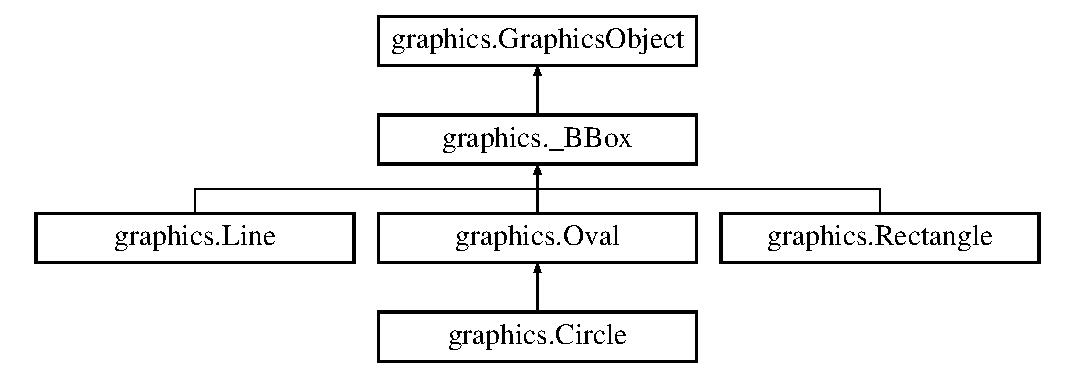
\includegraphics[height=4.000000cm]{classgraphics_1_1___b_box}
\end{center}
\end{figure}
\subsection*{Public Member Functions}
\begin{DoxyCompactItemize}
\item 
\mbox{\Hypertarget{classgraphics_1_1___b_box_a5738b02041db947dbbcb555ad6e6095a}\label{classgraphics_1_1___b_box_a5738b02041db947dbbcb555ad6e6095a}} 
def {\bfseries \+\_\+\+\_\+init\+\_\+\+\_\+} (self, p1, p2, options=\mbox{[}\char`\"{}outline\char`\"{}, width, fill)
\item 
\mbox{\Hypertarget{classgraphics_1_1___b_box_a2c3e73e8149fd0036055b94d28c3fbb4}\label{classgraphics_1_1___b_box_a2c3e73e8149fd0036055b94d28c3fbb4}} 
def {\bfseries get\+P1} (self)
\item 
\mbox{\Hypertarget{classgraphics_1_1___b_box_aee9d6dc9fcb9eb74ee8281662d87f361}\label{classgraphics_1_1___b_box_aee9d6dc9fcb9eb74ee8281662d87f361}} 
def {\bfseries get\+P2} (self)
\item 
\mbox{\Hypertarget{classgraphics_1_1___b_box_a7ffb5899c2626c1d882dae28b9eaf211}\label{classgraphics_1_1___b_box_a7ffb5899c2626c1d882dae28b9eaf211}} 
def {\bfseries get\+Center} (self)
\end{DoxyCompactItemize}
\subsection*{Public Attributes}
\begin{DoxyCompactItemize}
\item 
\mbox{\Hypertarget{classgraphics_1_1___b_box_a7d6ecb1b61e338a8f28e333c1e242b55}\label{classgraphics_1_1___b_box_a7d6ecb1b61e338a8f28e333c1e242b55}} 
{\bfseries p1}
\item 
\mbox{\Hypertarget{classgraphics_1_1___b_box_ae54a3cc11dc9be1624b0fbef0bf22d70}\label{classgraphics_1_1___b_box_ae54a3cc11dc9be1624b0fbef0bf22d70}} 
{\bfseries p2}
\end{DoxyCompactItemize}


The documentation for this class was generated from the following file\+:\begin{DoxyCompactItemize}
\item 
graphics.\+py\end{DoxyCompactItemize}

\hypertarget{classparser_classes_1_1_array}{}\section{parser\+Classes.\+Array Class Reference}
\label{classparser_classes_1_1_array}\index{parser\+Classes.\+Array@{parser\+Classes.\+Array}}


The documentation for this class was generated from the following file\+:\begin{DoxyCompactItemize}
\item 
parser\+Classes.\+py\end{DoxyCompactItemize}

\hypertarget{class_parsing_classes_actual_1_1_array}{}\section{Parsing\+Classes\+Actual.\+Array Class Reference}
\label{class_parsing_classes_actual_1_1_array}\index{Parsing\+Classes\+Actual.\+Array@{Parsing\+Classes\+Actual.\+Array}}


variable class of array which can be probed and updated  


\subsection*{Public Member Functions}
\begin{DoxyCompactItemize}
\item 
def \hyperlink{class_parsing_classes_actual_1_1_array_a749c8cc0cbee51cd8ac220c3afe4cccb}{\+\_\+\+\_\+init\+\_\+\+\_\+} (self, init\+Class, length, name)
\begin{DoxyCompactList}\small\item\em the constructor \end{DoxyCompactList}\item 
def \hyperlink{class_parsing_classes_actual_1_1_array_a0c67900f761bc072ed1f2a49ead7a0da}{get} (self, i)
\begin{DoxyCompactList}\small\item\em Gives the value of a variable at a particular index. \end{DoxyCompactList}\item 
def \hyperlink{class_parsing_classes_actual_1_1_array_a2a61097f1b529f1bdc8dcc4639e44414}{update} (self, i, value)
\begin{DoxyCompactList}\small\item\em Updates the value at a particular index. \end{DoxyCompactList}\end{DoxyCompactItemize}
\subsection*{Public Attributes}
\begin{DoxyCompactItemize}
\item 
{\bfseries name}\hypertarget{class_parsing_classes_actual_1_1_array_a0bc21e5ecf1ea116733950ea94fd355a}{}\label{class_parsing_classes_actual_1_1_array_a0bc21e5ecf1ea116733950ea94fd355a}

\item 
{\bfseries array}\hypertarget{class_parsing_classes_actual_1_1_array_a14c6e3eeac80e550ac15348387db7d4b}{}\label{class_parsing_classes_actual_1_1_array_a14c6e3eeac80e550ac15348387db7d4b}

\item 
{\bfseries length}\hypertarget{class_parsing_classes_actual_1_1_array_ac70adad351ea231f59e98c7df142e82c}{}\label{class_parsing_classes_actual_1_1_array_ac70adad351ea231f59e98c7df142e82c}

\end{DoxyCompactItemize}


\subsection{Detailed Description}
variable class of array which can be probed and updated 

\subsection{Constructor \& Destructor Documentation}
\index{Parsing\+Classes\+Actual\+::\+Array@{Parsing\+Classes\+Actual\+::\+Array}!\+\_\+\+\_\+init\+\_\+\+\_\+@{\+\_\+\+\_\+init\+\_\+\+\_\+}}
\index{\+\_\+\+\_\+init\+\_\+\+\_\+@{\+\_\+\+\_\+init\+\_\+\+\_\+}!Parsing\+Classes\+Actual\+::\+Array@{Parsing\+Classes\+Actual\+::\+Array}}
\subsubsection[{\texorpdfstring{\+\_\+\+\_\+init\+\_\+\+\_\+(self, init\+Class, length, name)}{__init__(self, initClass, length, name)}}]{\setlength{\rightskip}{0pt plus 5cm}def Parsing\+Classes\+Actual.\+Array.\+\_\+\+\_\+init\+\_\+\+\_\+ (
\begin{DoxyParamCaption}
\item[{}]{self, }
\item[{}]{init\+Class, }
\item[{}]{length, }
\item[{}]{name}
\end{DoxyParamCaption}
)}\hypertarget{class_parsing_classes_actual_1_1_array_a749c8cc0cbee51cd8ac220c3afe4cccb}{}\label{class_parsing_classes_actual_1_1_array_a749c8cc0cbee51cd8ac220c3afe4cccb}


the constructor 


\begin{DoxyParams}{Parameters}
{\em init\+Class} & The type of variable in array \\
\hline
{\em length} & The length of array \\
\hline
{\em name} & Name of array \\
\hline
\end{DoxyParams}


\subsection{Member Function Documentation}
\index{Parsing\+Classes\+Actual\+::\+Array@{Parsing\+Classes\+Actual\+::\+Array}!get@{get}}
\index{get@{get}!Parsing\+Classes\+Actual\+::\+Array@{Parsing\+Classes\+Actual\+::\+Array}}
\subsubsection[{\texorpdfstring{get(self, i)}{get(self, i)}}]{\setlength{\rightskip}{0pt plus 5cm}def Parsing\+Classes\+Actual.\+Array.\+get (
\begin{DoxyParamCaption}
\item[{}]{self, }
\item[{}]{i}
\end{DoxyParamCaption}
)}\hypertarget{class_parsing_classes_actual_1_1_array_a0c67900f761bc072ed1f2a49ead7a0da}{}\label{class_parsing_classes_actual_1_1_array_a0c67900f761bc072ed1f2a49ead7a0da}


Gives the value of a variable at a particular index. 


\begin{DoxyParams}{Parameters}
{\em i} & The index \\
\hline
\end{DoxyParams}
\index{Parsing\+Classes\+Actual\+::\+Array@{Parsing\+Classes\+Actual\+::\+Array}!update@{update}}
\index{update@{update}!Parsing\+Classes\+Actual\+::\+Array@{Parsing\+Classes\+Actual\+::\+Array}}
\subsubsection[{\texorpdfstring{update(self, i, value)}{update(self, i, value)}}]{\setlength{\rightskip}{0pt plus 5cm}def Parsing\+Classes\+Actual.\+Array.\+update (
\begin{DoxyParamCaption}
\item[{}]{self, }
\item[{}]{i, }
\item[{}]{value}
\end{DoxyParamCaption}
)}\hypertarget{class_parsing_classes_actual_1_1_array_a2a61097f1b529f1bdc8dcc4639e44414}{}\label{class_parsing_classes_actual_1_1_array_a2a61097f1b529f1bdc8dcc4639e44414}


Updates the value at a particular index. 


\begin{DoxyParams}{Parameters}
{\em i} & the index to be updated \\
\hline
{\em value} & the updated value \\
\hline
\end{DoxyParams}


The documentation for this class was generated from the following file\+:\begin{DoxyCompactItemize}
\item 
Parsing\+Classes\+Actual.\+py\end{DoxyCompactItemize}

\hypertarget{classparser_classes_1_1_array_declaration}{}\section{parser\+Classes.\+Array\+Declaration Class Reference}
\label{classparser_classes_1_1_array_declaration}\index{parser\+Classes.\+Array\+Declaration@{parser\+Classes.\+Array\+Declaration}}
\subsection*{Public Member Functions}
\begin{DoxyCompactItemize}
\item 
def {\bfseries \+\_\+\+\_\+init\+\_\+\+\_\+} (self, var\+Name, var\+Type, length, var\+Value)\hypertarget{classparser_classes_1_1_array_declaration_aa6752b68bcd3723ff304bf4cf5b24596}{}\label{classparser_classes_1_1_array_declaration_aa6752b68bcd3723ff304bf4cf5b24596}

\item 
def {\bfseries exec} (self)\hypertarget{classparser_classes_1_1_array_declaration_a73740b52f27f696a085be661cffaeabb}{}\label{classparser_classes_1_1_array_declaration_a73740b52f27f696a085be661cffaeabb}

\end{DoxyCompactItemize}
\subsection*{Public Attributes}
\begin{DoxyCompactItemize}
\item 
{\bfseries var\+Type}\hypertarget{classparser_classes_1_1_array_declaration_a17622e66df41a95f9b359700b7f8fbda}{}\label{classparser_classes_1_1_array_declaration_a17622e66df41a95f9b359700b7f8fbda}

\item 
{\bfseries length}\hypertarget{classparser_classes_1_1_array_declaration_a0c2efeb82bc5919dac3811d37ad4d8c9}{}\label{classparser_classes_1_1_array_declaration_a0c2efeb82bc5919dac3811d37ad4d8c9}

\item 
{\bfseries var\+Value}\hypertarget{classparser_classes_1_1_array_declaration_af4dc5a6cf288bce865fd7f198a3b3f71}{}\label{classparser_classes_1_1_array_declaration_af4dc5a6cf288bce865fd7f198a3b3f71}

\item 
{\bfseries var\+Name}\hypertarget{classparser_classes_1_1_array_declaration_a4070f5daf43664847cb46a8d4cafdf56}{}\label{classparser_classes_1_1_array_declaration_a4070f5daf43664847cb46a8d4cafdf56}

\end{DoxyCompactItemize}


The documentation for this class was generated from the following file\+:\begin{DoxyCompactItemize}
\item 
parser\+Classes.\+py\end{DoxyCompactItemize}

\hypertarget{class_parsing_classes_actual_1_1_array_declaration}{}\section{Parsing\+Classes\+Actual.\+Array\+Declaration Class Reference}
\label{class_parsing_classes_actual_1_1_array_declaration}\index{Parsing\+Classes\+Actual.\+Array\+Declaration@{Parsing\+Classes\+Actual.\+Array\+Declaration}}


the executable array declarartion  


\subsection*{Public Member Functions}
\begin{DoxyCompactItemize}
\item 
def \hyperlink{class_parsing_classes_actual_1_1_array_declaration_a3c5403f608468a688d68ae1f95a3569e}{\+\_\+\+\_\+init\+\_\+\+\_\+} (self, var\+Name, var\+Type, length, var\+Value, snippet)
\begin{DoxyCompactList}\small\item\em the constructor \end{DoxyCompactList}\item 
\mbox{\Hypertarget{class_parsing_classes_actual_1_1_array_declaration_a039a011fe347df7f8b5c9cb821839304}\label{class_parsing_classes_actual_1_1_array_declaration_a039a011fe347df7f8b5c9cb821839304}} 
def \hyperlink{class_parsing_classes_actual_1_1_array_declaration_a039a011fe347df7f8b5c9cb821839304}{exec} (self)
\begin{DoxyCompactList}\small\item\em The function which actually executes it. \end{DoxyCompactList}\end{DoxyCompactItemize}
\subsection*{Public Attributes}
\begin{DoxyCompactItemize}
\item 
\mbox{\Hypertarget{class_parsing_classes_actual_1_1_array_declaration_ab6f480c66cf067f1ecf0f9562449355d}\label{class_parsing_classes_actual_1_1_array_declaration_ab6f480c66cf067f1ecf0f9562449355d}} 
{\bfseries var\+Type}
\item 
\mbox{\Hypertarget{class_parsing_classes_actual_1_1_array_declaration_ae972ee9b5127dc41e06acda8f2c773d9}\label{class_parsing_classes_actual_1_1_array_declaration_ae972ee9b5127dc41e06acda8f2c773d9}} 
{\bfseries length}
\item 
\mbox{\Hypertarget{class_parsing_classes_actual_1_1_array_declaration_a9f5d5d01d5f35a289d1002a1205765a9}\label{class_parsing_classes_actual_1_1_array_declaration_a9f5d5d01d5f35a289d1002a1205765a9}} 
{\bfseries var\+Value}
\item 
\mbox{\Hypertarget{class_parsing_classes_actual_1_1_array_declaration_a0ce835763153799054bf9bbf08536419}\label{class_parsing_classes_actual_1_1_array_declaration_a0ce835763153799054bf9bbf08536419}} 
{\bfseries var\+Name}
\item 
\mbox{\Hypertarget{class_parsing_classes_actual_1_1_array_declaration_ac7ecc062ecd220e792a8e272bc86a6c1}\label{class_parsing_classes_actual_1_1_array_declaration_ac7ecc062ecd220e792a8e272bc86a6c1}} 
{\bfseries snippet}
\end{DoxyCompactItemize}


\subsection{Detailed Description}
the executable array declarartion 

\subsection{Constructor \& Destructor Documentation}
\mbox{\Hypertarget{class_parsing_classes_actual_1_1_array_declaration_a3c5403f608468a688d68ae1f95a3569e}\label{class_parsing_classes_actual_1_1_array_declaration_a3c5403f608468a688d68ae1f95a3569e}} 
\index{Parsing\+Classes\+Actual\+::\+Array\+Declaration@{Parsing\+Classes\+Actual\+::\+Array\+Declaration}!\+\_\+\+\_\+init\+\_\+\+\_\+@{\+\_\+\+\_\+init\+\_\+\+\_\+}}
\index{\+\_\+\+\_\+init\+\_\+\+\_\+@{\+\_\+\+\_\+init\+\_\+\+\_\+}!Parsing\+Classes\+Actual\+::\+Array\+Declaration@{Parsing\+Classes\+Actual\+::\+Array\+Declaration}}
\subsubsection{\texorpdfstring{\+\_\+\+\_\+init\+\_\+\+\_\+()}{\_\_init\_\_()}}
{\footnotesize\ttfamily def Parsing\+Classes\+Actual.\+Array\+Declaration.\+\_\+\+\_\+init\+\_\+\+\_\+ (\begin{DoxyParamCaption}\item[{}]{self,  }\item[{}]{var\+Name,  }\item[{}]{var\+Type,  }\item[{}]{length,  }\item[{}]{var\+Value,  }\item[{}]{snippet }\end{DoxyParamCaption})}



the constructor 


\begin{DoxyParams}{Parameters}
{\em var\+Name} & The name of the array \\
\hline
{\em var\+Type} & The type of the array elements \\
\hline
{\em length} & Length of the array \\
\hline
{\em var\+Value} & The value to which each element of array is to be initialized \\
\hline
{\em snippet} & the relevant snippet \\
\hline
\end{DoxyParams}


The documentation for this class was generated from the following file\+:\begin{DoxyCompactItemize}
\item 
Parsing\+Classes\+Actual.\+py\end{DoxyCompactItemize}

\hypertarget{classexecution_stack_1_1_array_node}{}\section{execution\+Stack.\+Array\+Node Class Reference}
\label{classexecution_stack_1_1_array_node}\index{execution\+Stack.\+Array\+Node@{execution\+Stack.\+Array\+Node}}
\subsection*{Public Member Functions}
\begin{DoxyCompactItemize}
\item 
def {\bfseries \+\_\+\+\_\+init\+\_\+\+\_\+} (self, x, y, val)\hypertarget{classexecution_stack_1_1_array_node_a77706dea871f1d386358a73040e5dea3}{}\label{classexecution_stack_1_1_array_node_a77706dea871f1d386358a73040e5dea3}

\item 
def {\bfseries update} (self, new\+Val)\hypertarget{classexecution_stack_1_1_array_node_ad2f67bb5aff43e472147fd8b6c437662}{}\label{classexecution_stack_1_1_array_node_ad2f67bb5aff43e472147fd8b6c437662}

\item 
def {\bfseries delete} (self)\hypertarget{classexecution_stack_1_1_array_node_ac61da4f274e4fdaf71cc76e1c77d21a0}{}\label{classexecution_stack_1_1_array_node_ac61da4f274e4fdaf71cc76e1c77d21a0}

\item 
def {\bfseries change\+Color} (self, color)\hypertarget{classexecution_stack_1_1_array_node_afe1ddcc32a2d47d16b16c39b9a79ecbc}{}\label{classexecution_stack_1_1_array_node_afe1ddcc32a2d47d16b16c39b9a79ecbc}

\end{DoxyCompactItemize}
\subsection*{Public Attributes}
\begin{DoxyCompactItemize}
\item 
{\bfseries data}\hypertarget{classexecution_stack_1_1_array_node_afb62811ca045506e06a377713425033b}{}\label{classexecution_stack_1_1_array_node_afb62811ca045506e06a377713425033b}

\item 
{\bfseries rectangle}\hypertarget{classexecution_stack_1_1_array_node_a94d21c229777c52da0d5552a7883821d}{}\label{classexecution_stack_1_1_array_node_a94d21c229777c52da0d5552a7883821d}

\item 
{\bfseries text}\hypertarget{classexecution_stack_1_1_array_node_ad4730d0b91ec85244f3e3e6bf6faf1a1}{}\label{classexecution_stack_1_1_array_node_ad4730d0b91ec85244f3e3e6bf6faf1a1}

\item 
{\bfseries val}\hypertarget{classexecution_stack_1_1_array_node_a95f1b1902891cf3fb239bece841e4bb5}{}\label{classexecution_stack_1_1_array_node_a95f1b1902891cf3fb239bece841e4bb5}

\end{DoxyCompactItemize}


The documentation for this class was generated from the following file\+:\begin{DoxyCompactItemize}
\item 
execution\+Stack.\+py\end{DoxyCompactItemize}

\hypertarget{classparser_classes_1_1_array_variable}{}\section{parser\+Classes.\+Array\+Variable Class Reference}
\label{classparser_classes_1_1_array_variable}\index{parser\+Classes.\+Array\+Variable@{parser\+Classes.\+Array\+Variable}}
\subsection*{Public Member Functions}
\begin{DoxyCompactItemize}
\item 
def {\bfseries \+\_\+\+\_\+init\+\_\+\+\_\+} (self, name, index)\hypertarget{classparser_classes_1_1_array_variable_afb6239db909b44d7ad42b79f1d89786d}{}\label{classparser_classes_1_1_array_variable_afb6239db909b44d7ad42b79f1d89786d}

\item 
def {\bfseries eval} (self)\hypertarget{classparser_classes_1_1_array_variable_a6c61b9b50fcaa606cc08af21d7f5778d}{}\label{classparser_classes_1_1_array_variable_a6c61b9b50fcaa606cc08af21d7f5778d}

\item 
def {\bfseries update} (self, value)\hypertarget{classparser_classes_1_1_array_variable_ae8068e5174714d900498f024a7933dca}{}\label{classparser_classes_1_1_array_variable_ae8068e5174714d900498f024a7933dca}

\end{DoxyCompactItemize}
\subsection*{Public Attributes}
\begin{DoxyCompactItemize}
\item 
{\bfseries name}\hypertarget{classparser_classes_1_1_array_variable_ad2e8e2f71b9333f55813166ae953e12e}{}\label{classparser_classes_1_1_array_variable_ad2e8e2f71b9333f55813166ae953e12e}

\item 
{\bfseries index}\hypertarget{classparser_classes_1_1_array_variable_a3a084b5d13c1e75b841842fe5bbf04c6}{}\label{classparser_classes_1_1_array_variable_a3a084b5d13c1e75b841842fe5bbf04c6}

\end{DoxyCompactItemize}


The documentation for this class was generated from the following file\+:\begin{DoxyCompactItemize}
\item 
parser\+Classes.\+py\end{DoxyCompactItemize}

\hypertarget{class_parsing_classes_actual_1_1_array_variable}{}\section{Parsing\+Classes\+Actual.\+Array\+Variable Class Reference}
\label{class_parsing_classes_actual_1_1_array_variable}\index{Parsing\+Classes\+Actual.\+Array\+Variable@{Parsing\+Classes\+Actual.\+Array\+Variable}}


The class which stores an array as a variable.  


\subsection*{Public Member Functions}
\begin{DoxyCompactItemize}
\item 
def \hyperlink{class_parsing_classes_actual_1_1_array_variable_a8d1f844a7bd0c87083039e7d40c5d882}{\+\_\+\+\_\+init\+\_\+\+\_\+} (self, name, index, snippet)
\begin{DoxyCompactList}\small\item\em The constructor which stores relevant parameters. \end{DoxyCompactList}\item 
def \hyperlink{class_parsing_classes_actual_1_1_array_variable_a1e14b4cc90b00fca48dbf6e9dcf58628}{eval} (self)\hypertarget{class_parsing_classes_actual_1_1_array_variable_a1e14b4cc90b00fca48dbf6e9dcf58628}{}\label{class_parsing_classes_actual_1_1_array_variable_a1e14b4cc90b00fca48dbf6e9dcf58628}

\begin{DoxyCompactList}\small\item\em The function which gives the value at that index. \end{DoxyCompactList}\item 
def \hyperlink{class_parsing_classes_actual_1_1_array_variable_adb73630679e22d44052196d2135b55bc}{update} (self, value)
\begin{DoxyCompactList}\small\item\em the function which updates the value at the stored index \end{DoxyCompactList}\end{DoxyCompactItemize}
\subsection*{Public Attributes}
\begin{DoxyCompactItemize}
\item 
{\bfseries name}\hypertarget{class_parsing_classes_actual_1_1_array_variable_a3d0632bea1f9f74b92f931cb941d06e7}{}\label{class_parsing_classes_actual_1_1_array_variable_a3d0632bea1f9f74b92f931cb941d06e7}

\item 
{\bfseries index}\hypertarget{class_parsing_classes_actual_1_1_array_variable_aa7cb30aa9447d819a00fa9ab2ce973d3}{}\label{class_parsing_classes_actual_1_1_array_variable_aa7cb30aa9447d819a00fa9ab2ce973d3}

\item 
{\bfseries snippet}\hypertarget{class_parsing_classes_actual_1_1_array_variable_aba5a945c50e696863b1bd4a68efb3b7f}{}\label{class_parsing_classes_actual_1_1_array_variable_aba5a945c50e696863b1bd4a68efb3b7f}

\end{DoxyCompactItemize}


\subsection{Detailed Description}
The class which stores an array as a variable. 

It is the basic class which holds the array value and the index which has to be either updated or evaluated acoording to the index at which it is 

\subsection{Constructor \& Destructor Documentation}
\index{Parsing\+Classes\+Actual\+::\+Array\+Variable@{Parsing\+Classes\+Actual\+::\+Array\+Variable}!\+\_\+\+\_\+init\+\_\+\+\_\+@{\+\_\+\+\_\+init\+\_\+\+\_\+}}
\index{\+\_\+\+\_\+init\+\_\+\+\_\+@{\+\_\+\+\_\+init\+\_\+\+\_\+}!Parsing\+Classes\+Actual\+::\+Array\+Variable@{Parsing\+Classes\+Actual\+::\+Array\+Variable}}
\subsubsection[{\texorpdfstring{\+\_\+\+\_\+init\+\_\+\+\_\+(self, name, index, snippet)}{__init__(self, name, index, snippet)}}]{\setlength{\rightskip}{0pt plus 5cm}def Parsing\+Classes\+Actual.\+Array\+Variable.\+\_\+\+\_\+init\+\_\+\+\_\+ (
\begin{DoxyParamCaption}
\item[{}]{self, }
\item[{}]{name, }
\item[{}]{index, }
\item[{}]{snippet}
\end{DoxyParamCaption}
)}\hypertarget{class_parsing_classes_actual_1_1_array_variable_a8d1f844a7bd0c87083039e7d40c5d882}{}\label{class_parsing_classes_actual_1_1_array_variable_a8d1f844a7bd0c87083039e7d40c5d882}


The constructor which stores relevant parameters. 


\begin{DoxyParams}{Parameters}
{\em name} & The name of the array variable \\
\hline
{\em index} & The index(a class that can be evaluated) of the array \\
\hline
{\em snippet} & The relevant code snippet \\
\hline
\end{DoxyParams}


\subsection{Member Function Documentation}
\index{Parsing\+Classes\+Actual\+::\+Array\+Variable@{Parsing\+Classes\+Actual\+::\+Array\+Variable}!update@{update}}
\index{update@{update}!Parsing\+Classes\+Actual\+::\+Array\+Variable@{Parsing\+Classes\+Actual\+::\+Array\+Variable}}
\subsubsection[{\texorpdfstring{update(self, value)}{update(self, value)}}]{\setlength{\rightskip}{0pt plus 5cm}def Parsing\+Classes\+Actual.\+Array\+Variable.\+update (
\begin{DoxyParamCaption}
\item[{}]{self, }
\item[{}]{value}
\end{DoxyParamCaption}
)}\hypertarget{class_parsing_classes_actual_1_1_array_variable_adb73630679e22d44052196d2135b55bc}{}\label{class_parsing_classes_actual_1_1_array_variable_adb73630679e22d44052196d2135b55bc}


the function which updates the value at the stored index 


\begin{DoxyParams}{Parameters}
{\em value} & The value(class that can be evaluated) to which the upation occurs \\
\hline
\end{DoxyParams}


The documentation for this class was generated from the following file\+:\begin{DoxyCompactItemize}
\item 
Parsing\+Classes\+Actual.\+py\end{DoxyCompactItemize}

\hypertarget{class_parsing_classes_actual_1_1_assignment}{}\section{Parsing\+Classes\+Actual.\+Assignment Class Reference}
\label{class_parsing_classes_actual_1_1_assignment}\index{Parsing\+Classes\+Actual.\+Assignment@{Parsing\+Classes\+Actual.\+Assignment}}


the executable class for assignment which contains the variable and the expression  


\subsection*{Public Member Functions}
\begin{DoxyCompactItemize}
\item 
def \hyperlink{class_parsing_classes_actual_1_1_assignment_ad1ed51f09df9ee3ca193e0a5f6646c11}{\+\_\+\+\_\+init\+\_\+\+\_\+} (self, left, right, snippet)
\begin{DoxyCompactList}\small\item\em the constructor \end{DoxyCompactList}\item 
def \hyperlink{class_parsing_classes_actual_1_1_assignment_ad9d41c2aca94f42213fed890eb33aa44}{exec} (self)\hypertarget{class_parsing_classes_actual_1_1_assignment_ad9d41c2aca94f42213fed890eb33aa44}{}\label{class_parsing_classes_actual_1_1_assignment_ad9d41c2aca94f42213fed890eb33aa44}

\begin{DoxyCompactList}\small\item\em The function which actually carries out the updation. \end{DoxyCompactList}\end{DoxyCompactItemize}
\subsection*{Public Attributes}
\begin{DoxyCompactItemize}
\item 
{\bfseries left}\hypertarget{class_parsing_classes_actual_1_1_assignment_ae9e7a7861ee3c433563e3ffb84e96136}{}\label{class_parsing_classes_actual_1_1_assignment_ae9e7a7861ee3c433563e3ffb84e96136}

\item 
{\bfseries right}\hypertarget{class_parsing_classes_actual_1_1_assignment_a47a5c7ff174dac880264b4bcac0cdb4c}{}\label{class_parsing_classes_actual_1_1_assignment_a47a5c7ff174dac880264b4bcac0cdb4c}

\item 
{\bfseries snippet}\hypertarget{class_parsing_classes_actual_1_1_assignment_aafc31dddf6dfff65459ef199c7c6b829}{}\label{class_parsing_classes_actual_1_1_assignment_aafc31dddf6dfff65459ef199c7c6b829}

\end{DoxyCompactItemize}


\subsection{Detailed Description}
the executable class for assignment which contains the variable and the expression 

\subsection{Constructor \& Destructor Documentation}
\index{Parsing\+Classes\+Actual\+::\+Assignment@{Parsing\+Classes\+Actual\+::\+Assignment}!\+\_\+\+\_\+init\+\_\+\+\_\+@{\+\_\+\+\_\+init\+\_\+\+\_\+}}
\index{\+\_\+\+\_\+init\+\_\+\+\_\+@{\+\_\+\+\_\+init\+\_\+\+\_\+}!Parsing\+Classes\+Actual\+::\+Assignment@{Parsing\+Classes\+Actual\+::\+Assignment}}
\subsubsection[{\texorpdfstring{\+\_\+\+\_\+init\+\_\+\+\_\+(self, left, right, snippet)}{__init__(self, left, right, snippet)}}]{\setlength{\rightskip}{0pt plus 5cm}def Parsing\+Classes\+Actual.\+Assignment.\+\_\+\+\_\+init\+\_\+\+\_\+ (
\begin{DoxyParamCaption}
\item[{}]{self, }
\item[{}]{left, }
\item[{}]{right, }
\item[{}]{snippet}
\end{DoxyParamCaption}
)}\hypertarget{class_parsing_classes_actual_1_1_assignment_ad1ed51f09df9ee3ca193e0a5f6646c11}{}\label{class_parsing_classes_actual_1_1_assignment_ad1ed51f09df9ee3ca193e0a5f6646c11}


the constructor 


\begin{DoxyParams}{Parameters}
{\em left} & The \hyperlink{class_parsing_classes_actual_1_1_variable}{Variable} class to be updated \\
\hline
{\em right} & the expression to be evaluated \\
\hline
{\em snippet} & The relevant code snippet \\
\hline
\end{DoxyParams}


The documentation for this class was generated from the following file\+:\begin{DoxyCompactItemize}
\item 
Parsing\+Classes\+Actual.\+py\end{DoxyCompactItemize}

\hypertarget{classparser_classes_1_1_assignment}{}\section{parser\+Classes.\+Assignment Class Reference}
\label{classparser_classes_1_1_assignment}\index{parser\+Classes.\+Assignment@{parser\+Classes.\+Assignment}}
\subsection*{Public Member Functions}
\begin{DoxyCompactItemize}
\item 
\mbox{\Hypertarget{classparser_classes_1_1_assignment_a43da5ff93b04c80d9a466dcebd309d00}\label{classparser_classes_1_1_assignment_a43da5ff93b04c80d9a466dcebd309d00}} 
def {\bfseries \+\_\+\+\_\+init\+\_\+\+\_\+} (self, left, right)
\item 
\mbox{\Hypertarget{classparser_classes_1_1_assignment_a3c1e04ff93d19320677466afea6365bb}\label{classparser_classes_1_1_assignment_a3c1e04ff93d19320677466afea6365bb}} 
def {\bfseries exec} (self)
\end{DoxyCompactItemize}
\subsection*{Public Attributes}
\begin{DoxyCompactItemize}
\item 
\mbox{\Hypertarget{classparser_classes_1_1_assignment_ae986cc4a7cfecdaa4e3f63d14dbe88ef}\label{classparser_classes_1_1_assignment_ae986cc4a7cfecdaa4e3f63d14dbe88ef}} 
{\bfseries left}
\item 
\mbox{\Hypertarget{classparser_classes_1_1_assignment_a422e2e0ef9731ceee7bc8ac30a226f1c}\label{classparser_classes_1_1_assignment_a422e2e0ef9731ceee7bc8ac30a226f1c}} 
{\bfseries right}
\end{DoxyCompactItemize}


The documentation for this class was generated from the following file\+:\begin{DoxyCompactItemize}
\item 
parser\+Classes.\+py\end{DoxyCompactItemize}

\hypertarget{class_parsing_classes_actual_1_1_binary_op}{}\section{Parsing\+Classes\+Actual.\+Binary\+Op Class Reference}
\label{class_parsing_classes_actual_1_1_binary_op}\index{Parsing\+Classes\+Actual.\+Binary\+Op@{Parsing\+Classes\+Actual.\+Binary\+Op}}


class for binary operator containg operands and the relevant function  


\subsection*{Public Member Functions}
\begin{DoxyCompactItemize}
\item 
def \hyperlink{class_parsing_classes_actual_1_1_binary_op_a3d8482575f41d191640a397be6806991}{\+\_\+\+\_\+init\+\_\+\+\_\+} (self, operator, left, right, snippet)
\begin{DoxyCompactList}\small\item\em The constructor. \end{DoxyCompactList}\item 
def \hyperlink{class_parsing_classes_actual_1_1_binary_op_a27757ec13077dda98775d2e3c6a29f65}{eval} (self)\hypertarget{class_parsing_classes_actual_1_1_binary_op_a27757ec13077dda98775d2e3c6a29f65}{}\label{class_parsing_classes_actual_1_1_binary_op_a27757ec13077dda98775d2e3c6a29f65}

\begin{DoxyCompactList}\small\item\em The function that returns the value on evaluating the expression. \end{DoxyCompactList}\item 
def \hyperlink{class_parsing_classes_actual_1_1_binary_op_a6ba5fdbdcda94f4f07e7d6c2f4438322}{exec} (self)\hypertarget{class_parsing_classes_actual_1_1_binary_op_a6ba5fdbdcda94f4f07e7d6c2f4438322}{}\label{class_parsing_classes_actual_1_1_binary_op_a6ba5fdbdcda94f4f07e7d6c2f4438322}

\begin{DoxyCompactList}\small\item\em it evaluates expression \end{DoxyCompactList}\item 
def \hyperlink{class_parsing_classes_actual_1_1_binary_op_ae926977b3df2b3567ccd6389e595d326}{get\+Operator} (self)\hypertarget{class_parsing_classes_actual_1_1_binary_op_ae926977b3df2b3567ccd6389e595d326}{}\label{class_parsing_classes_actual_1_1_binary_op_ae926977b3df2b3567ccd6389e595d326}

\begin{DoxyCompactList}\small\item\em returns the type of operator \end{DoxyCompactList}\end{DoxyCompactItemize}
\subsection*{Public Attributes}
\begin{DoxyCompactItemize}
\item 
{\bfseries operator}\hypertarget{class_parsing_classes_actual_1_1_binary_op_a4cd309c1dba26f392ccc0eec35713e36}{}\label{class_parsing_classes_actual_1_1_binary_op_a4cd309c1dba26f392ccc0eec35713e36}

\item 
{\bfseries left}\hypertarget{class_parsing_classes_actual_1_1_binary_op_ab5063aaba0e6111792dfc879ef0daf13}{}\label{class_parsing_classes_actual_1_1_binary_op_ab5063aaba0e6111792dfc879ef0daf13}

\item 
{\bfseries right}\hypertarget{class_parsing_classes_actual_1_1_binary_op_af9b2ba232bcc0cf4ec48ad68b12572f2}{}\label{class_parsing_classes_actual_1_1_binary_op_af9b2ba232bcc0cf4ec48ad68b12572f2}

\item 
{\bfseries snippet}\hypertarget{class_parsing_classes_actual_1_1_binary_op_a794e13c741129c2da81d9845b41e0df8}{}\label{class_parsing_classes_actual_1_1_binary_op_a794e13c741129c2da81d9845b41e0df8}

\end{DoxyCompactItemize}


\subsection{Detailed Description}
class for binary operator containg operands and the relevant function 

\subsection{Constructor \& Destructor Documentation}
\index{Parsing\+Classes\+Actual\+::\+Binary\+Op@{Parsing\+Classes\+Actual\+::\+Binary\+Op}!\+\_\+\+\_\+init\+\_\+\+\_\+@{\+\_\+\+\_\+init\+\_\+\+\_\+}}
\index{\+\_\+\+\_\+init\+\_\+\+\_\+@{\+\_\+\+\_\+init\+\_\+\+\_\+}!Parsing\+Classes\+Actual\+::\+Binary\+Op@{Parsing\+Classes\+Actual\+::\+Binary\+Op}}
\subsubsection[{\texorpdfstring{\+\_\+\+\_\+init\+\_\+\+\_\+(self, operator, left, right, snippet)}{__init__(self, operator, left, right, snippet)}}]{\setlength{\rightskip}{0pt plus 5cm}def Parsing\+Classes\+Actual.\+Binary\+Op.\+\_\+\+\_\+init\+\_\+\+\_\+ (
\begin{DoxyParamCaption}
\item[{}]{self, }
\item[{}]{operator, }
\item[{}]{left, }
\item[{}]{right, }
\item[{}]{snippet}
\end{DoxyParamCaption}
)}\hypertarget{class_parsing_classes_actual_1_1_binary_op_a3d8482575f41d191640a397be6806991}{}\label{class_parsing_classes_actual_1_1_binary_op_a3d8482575f41d191640a397be6806991}


The constructor. 


\begin{DoxyParams}{Parameters}
{\em operator} & The operation to be done between the values \\
\hline
{\em left} & Left side of operand \\
\hline
{\em right} & right side of operand \\
\hline
{\em snippet} & The relavant code snippet \\
\hline
\end{DoxyParams}


The documentation for this class was generated from the following file\+:\begin{DoxyCompactItemize}
\item 
Parsing\+Classes\+Actual.\+py\end{DoxyCompactItemize}

\hypertarget{classparser_classes_1_1_binary_op}{}\section{parser\+Classes.\+Binary\+Op Class Reference}
\label{classparser_classes_1_1_binary_op}\index{parser\+Classes.\+Binary\+Op@{parser\+Classes.\+Binary\+Op}}
\subsection*{Public Member Functions}
\begin{DoxyCompactItemize}
\item 
\mbox{\Hypertarget{classparser_classes_1_1_binary_op_a554daa9084dec66629f4b9582793555d}\label{classparser_classes_1_1_binary_op_a554daa9084dec66629f4b9582793555d}} 
def {\bfseries \+\_\+\+\_\+init\+\_\+\+\_\+} (self, operator, left, right)
\item 
\mbox{\Hypertarget{classparser_classes_1_1_binary_op_af5b9586e9192fbd0e829d4f514cd7647}\label{classparser_classes_1_1_binary_op_af5b9586e9192fbd0e829d4f514cd7647}} 
def {\bfseries eval} (self)
\item 
\mbox{\Hypertarget{classparser_classes_1_1_binary_op_a44c9156cf60631383bc9147b61604ba4}\label{classparser_classes_1_1_binary_op_a44c9156cf60631383bc9147b61604ba4}} 
def {\bfseries exec} (self)
\item 
\mbox{\Hypertarget{classparser_classes_1_1_binary_op_ae7a261476e32638d9ce21cc311c86a85}\label{classparser_classes_1_1_binary_op_ae7a261476e32638d9ce21cc311c86a85}} 
def {\bfseries get\+Operator} (self)
\end{DoxyCompactItemize}
\subsection*{Public Attributes}
\begin{DoxyCompactItemize}
\item 
\mbox{\Hypertarget{classparser_classes_1_1_binary_op_a4fd8150b750a4dcdaaccedc83ef3d679}\label{classparser_classes_1_1_binary_op_a4fd8150b750a4dcdaaccedc83ef3d679}} 
{\bfseries operator}
\item 
\mbox{\Hypertarget{classparser_classes_1_1_binary_op_acf5520d9ff520e7477caff66289a3206}\label{classparser_classes_1_1_binary_op_acf5520d9ff520e7477caff66289a3206}} 
{\bfseries left}
\item 
\mbox{\Hypertarget{classparser_classes_1_1_binary_op_a333e735c904ef6750472deba2fd9d85f}\label{classparser_classes_1_1_binary_op_a333e735c904ef6750472deba2fd9d85f}} 
{\bfseries right}
\end{DoxyCompactItemize}


The documentation for this class was generated from the following file\+:\begin{DoxyCompactItemize}
\item 
parser\+Classes.\+py\end{DoxyCompactItemize}

\hypertarget{class_binary_search_tree_1_1_binary_search_tree}{}\section{Binary\+Search\+Tree.\+Binary\+Search\+Tree Class Reference}
\label{class_binary_search_tree_1_1_binary_search_tree}\index{Binary\+Search\+Tree.\+Binary\+Search\+Tree@{Binary\+Search\+Tree.\+Binary\+Search\+Tree}}
\subsection*{Public Member Functions}
\begin{DoxyCompactItemize}
\item 
\mbox{\Hypertarget{class_binary_search_tree_1_1_binary_search_tree_a427e86bf2d372a1b518489843bc85103}\label{class_binary_search_tree_1_1_binary_search_tree_a427e86bf2d372a1b518489843bc85103}} 
def {\bfseries \+\_\+\+\_\+init\+\_\+\+\_\+} (self, x, y, model\+Type, name)
\item 
\mbox{\Hypertarget{class_binary_search_tree_1_1_binary_search_tree_a5168edcb8e13e75c4d9f9d016cf922e0}\label{class_binary_search_tree_1_1_binary_search_tree_a5168edcb8e13e75c4d9f9d016cf922e0}} 
def {\bfseries search\+Add} (self, node, val, level)
\item 
\mbox{\Hypertarget{class_binary_search_tree_1_1_binary_search_tree_a590449bc083a03f8746362ae21081c6b}\label{class_binary_search_tree_1_1_binary_search_tree_a590449bc083a03f8746362ae21081c6b}} 
def {\bfseries redraw} (self)
\item 
\mbox{\Hypertarget{class_binary_search_tree_1_1_binary_search_tree_a78d7a635850da8941d434365d6447f75}\label{class_binary_search_tree_1_1_binary_search_tree_a78d7a635850da8941d434365d6447f75}} 
def {\bfseries over\+Draw} (self, node)
\item 
\mbox{\Hypertarget{class_binary_search_tree_1_1_binary_search_tree_a64a520f74e40f705873893befbe905c3}\label{class_binary_search_tree_1_1_binary_search_tree_a64a520f74e40f705873893befbe905c3}} 
def {\bfseries make\+Lines} (self, node)
\item 
\mbox{\Hypertarget{class_binary_search_tree_1_1_binary_search_tree_ae3acf8c976ea9f9dd05d381954c430ed}\label{class_binary_search_tree_1_1_binary_search_tree_ae3acf8c976ea9f9dd05d381954c430ed}} 
def {\bfseries relocate} (self, node, x, y, level)
\item 
\mbox{\Hypertarget{class_binary_search_tree_1_1_binary_search_tree_ab410c124ca03f9cb2f8b7f72a1529196}\label{class_binary_search_tree_1_1_binary_search_tree_ab410c124ca03f9cb2f8b7f72a1529196}} 
def {\bfseries insert} (self, val)
\item 
\mbox{\Hypertarget{class_binary_search_tree_1_1_binary_search_tree_ae170d61050f5e183ef93ed650d8449d7}\label{class_binary_search_tree_1_1_binary_search_tree_ae170d61050f5e183ef93ed650d8449d7}} 
def {\bfseries search\+Helper} (self, node, val)
\item 
\mbox{\Hypertarget{class_binary_search_tree_1_1_binary_search_tree_ac04f7b8898dddd138c18e9e0bc7b68ad}\label{class_binary_search_tree_1_1_binary_search_tree_ac04f7b8898dddd138c18e9e0bc7b68ad}} 
def {\bfseries find\+Height} (self, node)
\item 
\mbox{\Hypertarget{class_binary_search_tree_1_1_binary_search_tree_a250e673d04491e5d995b08b36e10072d}\label{class_binary_search_tree_1_1_binary_search_tree_a250e673d04491e5d995b08b36e10072d}} 
def {\bfseries search} (self, val)
\item 
\mbox{\Hypertarget{class_binary_search_tree_1_1_binary_search_tree_a71d2af564255a83b5d11ed57d099c945}\label{class_binary_search_tree_1_1_binary_search_tree_a71d2af564255a83b5d11ed57d099c945}} 
def {\bfseries search\+Delete} (self, node, val)
\item 
\mbox{\Hypertarget{class_binary_search_tree_1_1_binary_search_tree_a27ef9920f4c1e30e4d27cc4191d763f5}\label{class_binary_search_tree_1_1_binary_search_tree_a27ef9920f4c1e30e4d27cc4191d763f5}} 
def {\bfseries find\+Leftmost} (self, node)
\item 
\mbox{\Hypertarget{class_binary_search_tree_1_1_binary_search_tree_ada4129c8eb622c9180596f7df720f4db}\label{class_binary_search_tree_1_1_binary_search_tree_ada4129c8eb622c9180596f7df720f4db}} 
def {\bfseries erase} (self, val)
\end{DoxyCompactItemize}
\subsection*{Public Attributes}
\begin{DoxyCompactItemize}
\item 
\mbox{\Hypertarget{class_binary_search_tree_1_1_binary_search_tree_a399ad4c8ba4b21962841a0895f4933a5}\label{class_binary_search_tree_1_1_binary_search_tree_a399ad4c8ba4b21962841a0895f4933a5}} 
{\bfseries root\+Location}
\item 
\mbox{\Hypertarget{class_binary_search_tree_1_1_binary_search_tree_a28336f9c105f55dd0242225f94491a08}\label{class_binary_search_tree_1_1_binary_search_tree_a28336f9c105f55dd0242225f94491a08}} 
{\bfseries type}
\item 
\mbox{\Hypertarget{class_binary_search_tree_1_1_binary_search_tree_a507e958f649521d8d853007eefe3149b}\label{class_binary_search_tree_1_1_binary_search_tree_a507e958f649521d8d853007eefe3149b}} 
{\bfseries name}
\item 
\mbox{\Hypertarget{class_binary_search_tree_1_1_binary_search_tree_a8bb002fc1b00983a2512240378a5ccc2}\label{class_binary_search_tree_1_1_binary_search_tree_a8bb002fc1b00983a2512240378a5ccc2}} 
{\bfseries height}
\item 
\mbox{\Hypertarget{class_binary_search_tree_1_1_binary_search_tree_a4aa0ee481a5c399dc220c4c2284c7884}\label{class_binary_search_tree_1_1_binary_search_tree_a4aa0ee481a5c399dc220c4c2284c7884}} 
{\bfseries root}
\item 
\mbox{\Hypertarget{class_binary_search_tree_1_1_binary_search_tree_af6103954606e866294ab429e5b24aa01}\label{class_binary_search_tree_1_1_binary_search_tree_af6103954606e866294ab429e5b24aa01}} 
{\bfseries root\+Text}
\end{DoxyCompactItemize}


The documentation for this class was generated from the following file\+:\begin{DoxyCompactItemize}
\item 
Binary\+Search\+Tree.\+py\end{DoxyCompactItemize}

\hypertarget{class_binary_search_tree_1_1_binary_tree_node}{}\section{Binary\+Search\+Tree.\+Binary\+Tree\+Node Class Reference}
\label{class_binary_search_tree_1_1_binary_tree_node}\index{Binary\+Search\+Tree.\+Binary\+Tree\+Node@{Binary\+Search\+Tree.\+Binary\+Tree\+Node}}


Class which stores all the graphical information and data related to a node in a binary tree.  


\subsection*{Public Member Functions}
\begin{DoxyCompactItemize}
\item 
def \hyperlink{class_binary_search_tree_1_1_binary_tree_node_a82eeb27919e933cb0bbab2bb19a4674a}{\+\_\+\+\_\+init\+\_\+\+\_\+} (self, lchild, rchild, val, x, y)
\begin{DoxyCompactList}\small\item\em Constructor for the class. \end{DoxyCompactList}\item 
def \hyperlink{class_binary_search_tree_1_1_binary_tree_node_aa7b30f6a083e5eb57d4048c6a83bfff1}{relocate} (self, x, y)
\begin{DoxyCompactList}\small\item\em Function to relocate the node to another point on the canvas. \end{DoxyCompactList}\item 
def \hyperlink{class_binary_search_tree_1_1_binary_tree_node_ab9dc94fd42e8ef8e1d7f5d5e62bb613a}{change\+Color} (self, color)
\begin{DoxyCompactList}\small\item\em Function to change the color of the node. \end{DoxyCompactList}\item 
\mbox{\Hypertarget{class_binary_search_tree_1_1_binary_tree_node_a4697a030e64bcc4abf33c3c1e10febbd}\label{class_binary_search_tree_1_1_binary_tree_node_a4697a030e64bcc4abf33c3c1e10febbd}} 
def \hyperlink{class_binary_search_tree_1_1_binary_tree_node_a4697a030e64bcc4abf33c3c1e10febbd}{delete} (self)
\begin{DoxyCompactList}\small\item\em Function to undraw the node and delete its contents. \end{DoxyCompactList}\item 
def \hyperlink{class_binary_search_tree_1_1_binary_tree_node_af69ab5e5100d035c4808ce89e2e6e835}{change\+Left} (self, lchild)
\begin{DoxyCompactList}\small\item\em Function to change the left child of the node along with all required graphical changes. \end{DoxyCompactList}\item 
def \hyperlink{class_binary_search_tree_1_1_binary_tree_node_a630b102ad6c1ccbdca6fd3b8f19260db}{change\+Right} (self, rchild)
\begin{DoxyCompactList}\small\item\em Function to change the right child of the node along with all required graphical changes. \end{DoxyCompactList}\item 
\mbox{\Hypertarget{class_binary_search_tree_1_1_binary_tree_node_a4be9ddca35a93613097f04ce6be9847c}\label{class_binary_search_tree_1_1_binary_tree_node_a4be9ddca35a93613097f04ce6be9847c}} 
def \hyperlink{class_binary_search_tree_1_1_binary_tree_node_a4be9ddca35a93613097f04ce6be9847c}{probe} (self)
\begin{DoxyCompactList}\small\item\em Function to change the color of a node to show that it is being probed. \end{DoxyCompactList}\item 
\mbox{\Hypertarget{class_binary_search_tree_1_1_binary_tree_node_a13edd0042d0de74ee2a9183c2ee4f73b}\label{class_binary_search_tree_1_1_binary_tree_node_a13edd0042d0de74ee2a9183c2ee4f73b}} 
def \hyperlink{class_binary_search_tree_1_1_binary_tree_node_a13edd0042d0de74ee2a9183c2ee4f73b}{redraw} (self)
\begin{DoxyCompactList}\small\item\em Function to redraw the node. \end{DoxyCompactList}\item 
\mbox{\Hypertarget{class_binary_search_tree_1_1_binary_tree_node_a4697a030e64bcc4abf33c3c1e10febbd}\label{class_binary_search_tree_1_1_binary_tree_node_a4697a030e64bcc4abf33c3c1e10febbd}} 
def \hyperlink{class_binary_search_tree_1_1_binary_tree_node_a4697a030e64bcc4abf33c3c1e10febbd}{delete} (self)
\begin{DoxyCompactList}\small\item\em Function to change the color of the node and then delete it. \end{DoxyCompactList}\end{DoxyCompactItemize}
\subsection*{Public Attributes}
\begin{DoxyCompactItemize}
\item 
\mbox{\Hypertarget{class_binary_search_tree_1_1_binary_tree_node_a2a7329ecef9597b0639d5e56d1fb9e98}\label{class_binary_search_tree_1_1_binary_tree_node_a2a7329ecef9597b0639d5e56d1fb9e98}} 
{\bfseries left}
\item 
\mbox{\Hypertarget{class_binary_search_tree_1_1_binary_tree_node_a8ec787cb980f443ef91e36adbc07f03b}\label{class_binary_search_tree_1_1_binary_tree_node_a8ec787cb980f443ef91e36adbc07f03b}} 
{\bfseries right}
\item 
\mbox{\Hypertarget{class_binary_search_tree_1_1_binary_tree_node_a7dc751865b03d93d7a2eaf8e0453021f}\label{class_binary_search_tree_1_1_binary_tree_node_a7dc751865b03d93d7a2eaf8e0453021f}} 
{\bfseries data}
\item 
\mbox{\Hypertarget{class_binary_search_tree_1_1_binary_tree_node_a06a5a777f647a7fd179e98e6908fb7c9}\label{class_binary_search_tree_1_1_binary_tree_node_a06a5a777f647a7fd179e98e6908fb7c9}} 
{\bfseries circle}
\item 
\mbox{\Hypertarget{class_binary_search_tree_1_1_binary_tree_node_a5105a9ac24008de97b2243aa8ceb9566}\label{class_binary_search_tree_1_1_binary_tree_node_a5105a9ac24008de97b2243aa8ceb9566}} 
{\bfseries location}
\item 
\mbox{\Hypertarget{class_binary_search_tree_1_1_binary_tree_node_acc17cecd9513b2d26b8b1c777d72407f}\label{class_binary_search_tree_1_1_binary_tree_node_acc17cecd9513b2d26b8b1c777d72407f}} 
{\bfseries text}
\item 
\mbox{\Hypertarget{class_binary_search_tree_1_1_binary_tree_node_abef335231af642d070f64122033f2ff7}\label{class_binary_search_tree_1_1_binary_tree_node_abef335231af642d070f64122033f2ff7}} 
{\bfseries left\+Line}
\item 
\mbox{\Hypertarget{class_binary_search_tree_1_1_binary_tree_node_a2fb1088533007be5718735e39080f6c9}\label{class_binary_search_tree_1_1_binary_tree_node_a2fb1088533007be5718735e39080f6c9}} 
{\bfseries right\+Line}
\end{DoxyCompactItemize}


\subsection{Detailed Description}
Class which stores all the graphical information and data related to a node in a binary tree. 

\subsection{Constructor \& Destructor Documentation}
\mbox{\Hypertarget{class_binary_search_tree_1_1_binary_tree_node_a82eeb27919e933cb0bbab2bb19a4674a}\label{class_binary_search_tree_1_1_binary_tree_node_a82eeb27919e933cb0bbab2bb19a4674a}} 
\index{Binary\+Search\+Tree\+::\+Binary\+Tree\+Node@{Binary\+Search\+Tree\+::\+Binary\+Tree\+Node}!\+\_\+\+\_\+init\+\_\+\+\_\+@{\+\_\+\+\_\+init\+\_\+\+\_\+}}
\index{\+\_\+\+\_\+init\+\_\+\+\_\+@{\+\_\+\+\_\+init\+\_\+\+\_\+}!Binary\+Search\+Tree\+::\+Binary\+Tree\+Node@{Binary\+Search\+Tree\+::\+Binary\+Tree\+Node}}
\subsubsection{\texorpdfstring{\+\_\+\+\_\+init\+\_\+\+\_\+()}{\_\_init\_\_()}}
{\footnotesize\ttfamily def Binary\+Search\+Tree.\+Binary\+Tree\+Node.\+\_\+\+\_\+init\+\_\+\+\_\+ (\begin{DoxyParamCaption}\item[{}]{self,  }\item[{}]{lchild,  }\item[{}]{rchild,  }\item[{}]{val,  }\item[{}]{x,  }\item[{}]{y }\end{DoxyParamCaption})}



Constructor for the class. 


\begin{DoxyParams}{Parameters}
{\em lchild} & -\/ the left child of the node in the tree \\
\hline
{\em rchild} & -\/ the right child of the node in the tree \\
\hline
{\em val} & -\/ the value to be stored in the node \\
\hline
{\em x} & -\/ the x coordinate of the centre of the node \\
\hline
{\em y} & -\/ the y coordinate of the centre of the node \\
\hline
\end{DoxyParams}


\subsection{Member Function Documentation}
\mbox{\Hypertarget{class_binary_search_tree_1_1_binary_tree_node_ab9dc94fd42e8ef8e1d7f5d5e62bb613a}\label{class_binary_search_tree_1_1_binary_tree_node_ab9dc94fd42e8ef8e1d7f5d5e62bb613a}} 
\index{Binary\+Search\+Tree\+::\+Binary\+Tree\+Node@{Binary\+Search\+Tree\+::\+Binary\+Tree\+Node}!change\+Color@{change\+Color}}
\index{change\+Color@{change\+Color}!Binary\+Search\+Tree\+::\+Binary\+Tree\+Node@{Binary\+Search\+Tree\+::\+Binary\+Tree\+Node}}
\subsubsection{\texorpdfstring{change\+Color()}{changeColor()}}
{\footnotesize\ttfamily def Binary\+Search\+Tree.\+Binary\+Tree\+Node.\+change\+Color (\begin{DoxyParamCaption}\item[{}]{self,  }\item[{}]{color }\end{DoxyParamCaption})}



Function to change the color of the node. 

-\/ the new color to be set as the background of the node \mbox{\Hypertarget{class_binary_search_tree_1_1_binary_tree_node_af69ab5e5100d035c4808ce89e2e6e835}\label{class_binary_search_tree_1_1_binary_tree_node_af69ab5e5100d035c4808ce89e2e6e835}} 
\index{Binary\+Search\+Tree\+::\+Binary\+Tree\+Node@{Binary\+Search\+Tree\+::\+Binary\+Tree\+Node}!change\+Left@{change\+Left}}
\index{change\+Left@{change\+Left}!Binary\+Search\+Tree\+::\+Binary\+Tree\+Node@{Binary\+Search\+Tree\+::\+Binary\+Tree\+Node}}
\subsubsection{\texorpdfstring{change\+Left()}{changeLeft()}}
{\footnotesize\ttfamily def Binary\+Search\+Tree.\+Binary\+Tree\+Node.\+change\+Left (\begin{DoxyParamCaption}\item[{}]{self,  }\item[{}]{lchild }\end{DoxyParamCaption})}



Function to change the left child of the node along with all required graphical changes. 


\begin{DoxyParams}{Parameters}
{\em lchild} & -\/ the new left child of the node \\
\hline
\end{DoxyParams}
\mbox{\Hypertarget{class_binary_search_tree_1_1_binary_tree_node_a630b102ad6c1ccbdca6fd3b8f19260db}\label{class_binary_search_tree_1_1_binary_tree_node_a630b102ad6c1ccbdca6fd3b8f19260db}} 
\index{Binary\+Search\+Tree\+::\+Binary\+Tree\+Node@{Binary\+Search\+Tree\+::\+Binary\+Tree\+Node}!change\+Right@{change\+Right}}
\index{change\+Right@{change\+Right}!Binary\+Search\+Tree\+::\+Binary\+Tree\+Node@{Binary\+Search\+Tree\+::\+Binary\+Tree\+Node}}
\subsubsection{\texorpdfstring{change\+Right()}{changeRight()}}
{\footnotesize\ttfamily def Binary\+Search\+Tree.\+Binary\+Tree\+Node.\+change\+Right (\begin{DoxyParamCaption}\item[{}]{self,  }\item[{}]{rchild }\end{DoxyParamCaption})}



Function to change the right child of the node along with all required graphical changes. 


\begin{DoxyParams}{Parameters}
{\em rchild} & -\/ the new right child of the node \\
\hline
\end{DoxyParams}
\mbox{\Hypertarget{class_binary_search_tree_1_1_binary_tree_node_aa7b30f6a083e5eb57d4048c6a83bfff1}\label{class_binary_search_tree_1_1_binary_tree_node_aa7b30f6a083e5eb57d4048c6a83bfff1}} 
\index{Binary\+Search\+Tree\+::\+Binary\+Tree\+Node@{Binary\+Search\+Tree\+::\+Binary\+Tree\+Node}!relocate@{relocate}}
\index{relocate@{relocate}!Binary\+Search\+Tree\+::\+Binary\+Tree\+Node@{Binary\+Search\+Tree\+::\+Binary\+Tree\+Node}}
\subsubsection{\texorpdfstring{relocate()}{relocate()}}
{\footnotesize\ttfamily def Binary\+Search\+Tree.\+Binary\+Tree\+Node.\+relocate (\begin{DoxyParamCaption}\item[{}]{self,  }\item[{}]{x,  }\item[{}]{y }\end{DoxyParamCaption})}



Function to relocate the node to another point on the canvas. 


\begin{DoxyParams}{Parameters}
{\em x} & -\/ the new x coordinate \\
\hline
{\em y} & -\/ the new y coordinate \\
\hline
\end{DoxyParams}


The documentation for this class was generated from the following file\+:\begin{DoxyCompactItemize}
\item 
Binary\+Search\+Tree.\+py\end{DoxyCompactItemize}

\hypertarget{class_parsing_classes_actual_1_1_block}{}\section{Parsing\+Classes\+Actual.\+Block Class Reference}
\label{class_parsing_classes_actual_1_1_block}\index{Parsing\+Classes\+Actual.\+Block@{Parsing\+Classes\+Actual.\+Block}}


the basic block containing list of executable statements that can be run  


\subsection*{Public Member Functions}
\begin{DoxyCompactItemize}
\item 
def \hyperlink{class_parsing_classes_actual_1_1_block_ac422058e3330cd4d72e14a3691037415}{\+\_\+\+\_\+init\+\_\+\+\_\+} (self, list\+Executables)
\begin{DoxyCompactList}\small\item\em the constructor \end{DoxyCompactList}\item 
\mbox{\Hypertarget{class_parsing_classes_actual_1_1_block_a9023ee93ba05105f1f9fe5f3014c347f}\label{class_parsing_classes_actual_1_1_block_a9023ee93ba05105f1f9fe5f3014c347f}} 
def \hyperlink{class_parsing_classes_actual_1_1_block_a9023ee93ba05105f1f9fe5f3014c347f}{exec} (self)
\begin{DoxyCompactList}\small\item\em the executable which exectutes all statement in a list until a return statement is encountered, on which that value is returned \end{DoxyCompactList}\end{DoxyCompactItemize}
\subsection*{Public Attributes}
\begin{DoxyCompactItemize}
\item 
\mbox{\Hypertarget{class_parsing_classes_actual_1_1_block_aac2c93f155a9e39693fd55cf62c5003d}\label{class_parsing_classes_actual_1_1_block_aac2c93f155a9e39693fd55cf62c5003d}} 
{\bfseries list\+Executables}
\end{DoxyCompactItemize}


\subsection{Detailed Description}
the basic block containing list of executable statements that can be run 

\subsection{Constructor \& Destructor Documentation}
\mbox{\Hypertarget{class_parsing_classes_actual_1_1_block_ac422058e3330cd4d72e14a3691037415}\label{class_parsing_classes_actual_1_1_block_ac422058e3330cd4d72e14a3691037415}} 
\index{Parsing\+Classes\+Actual\+::\+Block@{Parsing\+Classes\+Actual\+::\+Block}!\+\_\+\+\_\+init\+\_\+\+\_\+@{\+\_\+\+\_\+init\+\_\+\+\_\+}}
\index{\+\_\+\+\_\+init\+\_\+\+\_\+@{\+\_\+\+\_\+init\+\_\+\+\_\+}!Parsing\+Classes\+Actual\+::\+Block@{Parsing\+Classes\+Actual\+::\+Block}}
\subsubsection{\texorpdfstring{\+\_\+\+\_\+init\+\_\+\+\_\+()}{\_\_init\_\_()}}
{\footnotesize\ttfamily def Parsing\+Classes\+Actual.\+Block.\+\_\+\+\_\+init\+\_\+\+\_\+ (\begin{DoxyParamCaption}\item[{}]{self,  }\item[{}]{list\+Executables }\end{DoxyParamCaption})}



the constructor 


\begin{DoxyParams}{Parameters}
{\em the} & list of executable statement \\
\hline
\end{DoxyParams}


The documentation for this class was generated from the following file\+:\begin{DoxyCompactItemize}
\item 
Parsing\+Classes\+Actual.\+py\end{DoxyCompactItemize}

\hypertarget{classparser_classes_1_1_block}{}\section{parser\+Classes.\+Block Class Reference}
\label{classparser_classes_1_1_block}\index{parser\+Classes.\+Block@{parser\+Classes.\+Block}}
\subsection*{Public Member Functions}
\begin{DoxyCompactItemize}
\item 
def {\bfseries \+\_\+\+\_\+init\+\_\+\+\_\+} (self, list\+Executables)\hypertarget{classparser_classes_1_1_block_abcf2dbcf84fade861fdb6796668d7665}{}\label{classparser_classes_1_1_block_abcf2dbcf84fade861fdb6796668d7665}

\item 
def {\bfseries exec} (self)\hypertarget{classparser_classes_1_1_block_a4c3aaea61e8faeb4f83f3c534f6033f7}{}\label{classparser_classes_1_1_block_a4c3aaea61e8faeb4f83f3c534f6033f7}

\end{DoxyCompactItemize}
\subsection*{Public Attributes}
\begin{DoxyCompactItemize}
\item 
{\bfseries list\+Executables}\hypertarget{classparser_classes_1_1_block_ae6432948928c58e55813c7ea09f839ad}{}\label{classparser_classes_1_1_block_ae6432948928c58e55813c7ea09f839ad}

\end{DoxyCompactItemize}


The documentation for this class was generated from the following file\+:\begin{DoxyCompactItemize}
\item 
parser\+Classes.\+py\end{DoxyCompactItemize}

\hypertarget{class_parsing_classes_actual_1_1_bool}{}\section{Parsing\+Classes\+Actual.\+Bool Class Reference}
\label{class_parsing_classes_actual_1_1_bool}\index{Parsing\+Classes\+Actual.\+Bool@{Parsing\+Classes\+Actual.\+Bool}}


class for bool datatype  


Inheritance diagram for Parsing\+Classes\+Actual.\+Bool\+:\begin{figure}[H]
\begin{center}
\leavevmode
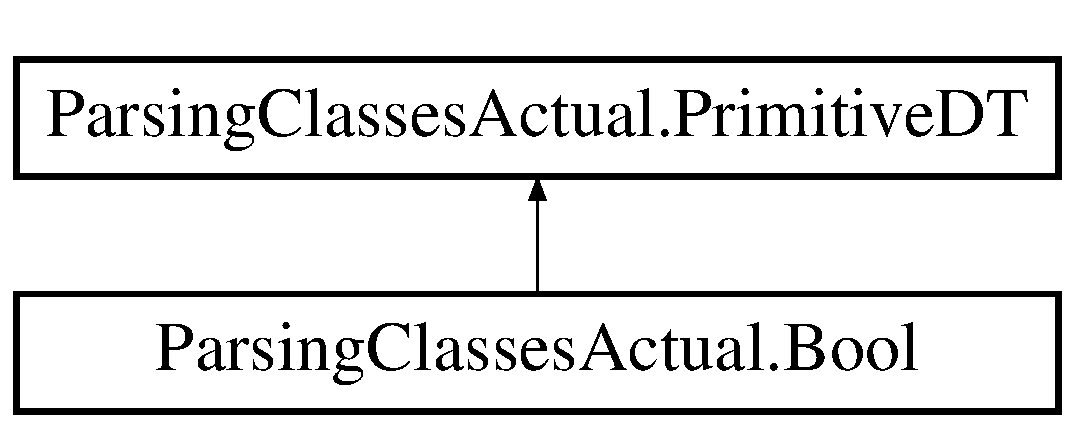
\includegraphics[height=2.000000cm]{class_parsing_classes_actual_1_1_bool}
\end{center}
\end{figure}
\subsection*{Public Member Functions}
\begin{DoxyCompactItemize}
\item 
def \hyperlink{class_parsing_classes_actual_1_1_bool_aff31c651efc789989951939a86fcc028}{\+\_\+\+\_\+init\+\_\+\+\_\+} (self, value=False)
\begin{DoxyCompactList}\small\item\em the constructor \end{DoxyCompactList}\item 
\mbox{\Hypertarget{class_parsing_classes_actual_1_1_bool_a1fca505331a7ee21f805b4975058f2ee}\label{class_parsing_classes_actual_1_1_bool_a1fca505331a7ee21f805b4975058f2ee}} 
def \hyperlink{class_parsing_classes_actual_1_1_bool_a1fca505331a7ee21f805b4975058f2ee}{give\+Type} (self)
\begin{DoxyCompactList}\small\item\em returns the type of value \end{DoxyCompactList}\item 
\mbox{\Hypertarget{class_parsing_classes_actual_1_1_bool_adde1b520ce9cc387ebefb158b984060b}\label{class_parsing_classes_actual_1_1_bool_adde1b520ce9cc387ebefb158b984060b}} 
def \hyperlink{class_parsing_classes_actual_1_1_bool_adde1b520ce9cc387ebefb158b984060b}{update} (self, val)
\begin{DoxyCompactList}\small\item\em updates the stored value by typecasting it \end{DoxyCompactList}\end{DoxyCompactItemize}
\subsection*{Public Attributes}
\begin{DoxyCompactItemize}
\item 
\mbox{\Hypertarget{class_parsing_classes_actual_1_1_bool_a7ed07bd1a1ca36b2378a72207546133c}\label{class_parsing_classes_actual_1_1_bool_a7ed07bd1a1ca36b2378a72207546133c}} 
{\bfseries value}
\end{DoxyCompactItemize}


\subsection{Detailed Description}
class for bool datatype 

\subsection{Constructor \& Destructor Documentation}
\mbox{\Hypertarget{class_parsing_classes_actual_1_1_bool_aff31c651efc789989951939a86fcc028}\label{class_parsing_classes_actual_1_1_bool_aff31c651efc789989951939a86fcc028}} 
\index{Parsing\+Classes\+Actual\+::\+Bool@{Parsing\+Classes\+Actual\+::\+Bool}!\+\_\+\+\_\+init\+\_\+\+\_\+@{\+\_\+\+\_\+init\+\_\+\+\_\+}}
\index{\+\_\+\+\_\+init\+\_\+\+\_\+@{\+\_\+\+\_\+init\+\_\+\+\_\+}!Parsing\+Classes\+Actual\+::\+Bool@{Parsing\+Classes\+Actual\+::\+Bool}}
\subsubsection{\texorpdfstring{\+\_\+\+\_\+init\+\_\+\+\_\+()}{\_\_init\_\_()}}
{\footnotesize\ttfamily def Parsing\+Classes\+Actual.\+Bool.\+\_\+\+\_\+init\+\_\+\+\_\+ (\begin{DoxyParamCaption}\item[{}]{self,  }\item[{}]{value = {\ttfamily False} }\end{DoxyParamCaption})}



the constructor 


\begin{DoxyParams}{Parameters}
{\em the} & value of datatype \\
\hline
\end{DoxyParams}


The documentation for this class was generated from the following file\+:\begin{DoxyCompactItemize}
\item 
Parsing\+Classes\+Actual.\+py\end{DoxyCompactItemize}

\hypertarget{classparser_classes_1_1_bool}{}\section{parser\+Classes.\+Bool Class Reference}
\label{classparser_classes_1_1_bool}\index{parser\+Classes.\+Bool@{parser\+Classes.\+Bool}}
Inheritance diagram for parser\+Classes.\+Bool\+:\begin{figure}[H]
\begin{center}
\leavevmode
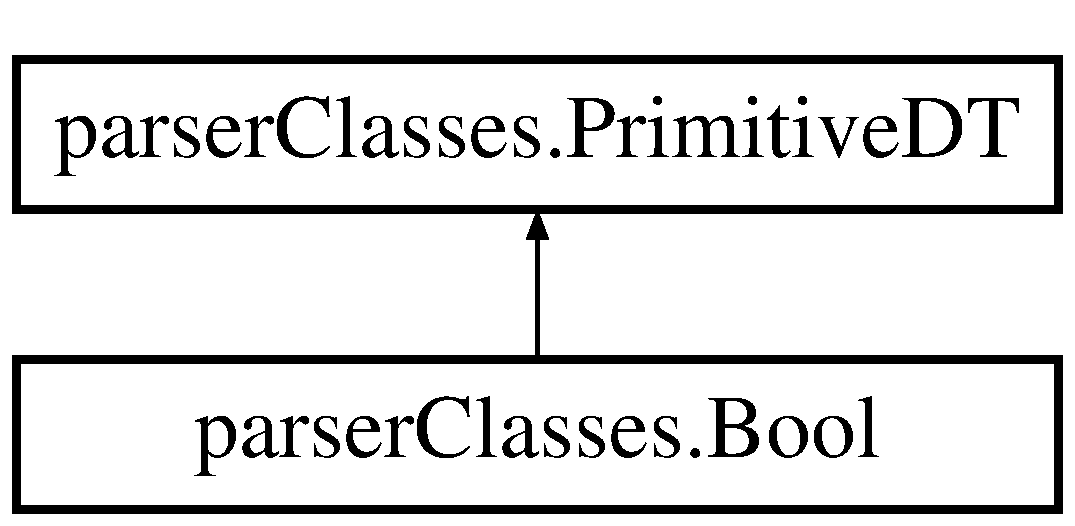
\includegraphics[height=2.000000cm]{classparser_classes_1_1_bool}
\end{center}
\end{figure}
\subsection*{Public Member Functions}
\begin{DoxyCompactItemize}
\item 
\mbox{\Hypertarget{classparser_classes_1_1_bool_aea596343fcf5032e9d9900cbe01402a5}\label{classparser_classes_1_1_bool_aea596343fcf5032e9d9900cbe01402a5}} 
def {\bfseries \+\_\+\+\_\+init\+\_\+\+\_\+} (self, value=False)
\item 
\mbox{\Hypertarget{classparser_classes_1_1_bool_a75f6909f270b96cceb0ff893d28e83c1}\label{classparser_classes_1_1_bool_a75f6909f270b96cceb0ff893d28e83c1}} 
def {\bfseries give\+Type} (self)
\item 
\mbox{\Hypertarget{classparser_classes_1_1_bool_a0d8251d04d4402acc11de38fe599fb12}\label{classparser_classes_1_1_bool_a0d8251d04d4402acc11de38fe599fb12}} 
def {\bfseries update} (self, val)
\end{DoxyCompactItemize}
\subsection*{Public Attributes}
\begin{DoxyCompactItemize}
\item 
\mbox{\Hypertarget{classparser_classes_1_1_bool_ab05879f8663a2e6ecb4a2dec445cbed0}\label{classparser_classes_1_1_bool_ab05879f8663a2e6ecb4a2dec445cbed0}} 
{\bfseries value}
\end{DoxyCompactItemize}


The documentation for this class was generated from the following file\+:\begin{DoxyCompactItemize}
\item 
parser\+Classes.\+py\end{DoxyCompactItemize}

\hypertarget{class_parsing_classes_actual_1_1_cin_statement}{}\section{Parsing\+Classes\+Actual.\+Cin\+Statement Class Reference}
\label{class_parsing_classes_actual_1_1_cin_statement}\index{Parsing\+Classes\+Actual.\+Cin\+Statement@{Parsing\+Classes\+Actual.\+Cin\+Statement}}


class for cin statement  


\subsection*{Public Member Functions}
\begin{DoxyCompactItemize}
\item 
def \hyperlink{class_parsing_classes_actual_1_1_cin_statement_a33f554b86027e75caf334cdf023d357f}{\+\_\+\+\_\+init\+\_\+\+\_\+} (self, list\+Of\+Vars, snippet)
\begin{DoxyCompactList}\small\item\em the constructor \end{DoxyCompactList}\item 
def \hyperlink{class_parsing_classes_actual_1_1_cin_statement_a29fcb8d0a00fc0dc615ba23c0a9f6487}{exec} (self)\hypertarget{class_parsing_classes_actual_1_1_cin_statement_a29fcb8d0a00fc0dc615ba23c0a9f6487}{}\label{class_parsing_classes_actual_1_1_cin_statement_a29fcb8d0a00fc0dc615ba23c0a9f6487}

\begin{DoxyCompactList}\small\item\em the executable that takes the input \end{DoxyCompactList}\end{DoxyCompactItemize}
\subsection*{Public Attributes}
\begin{DoxyCompactItemize}
\item 
{\bfseries list\+Of\+Vars}\hypertarget{class_parsing_classes_actual_1_1_cin_statement_acaf94d5b9909e8ba0aca2b95f4a78864}{}\label{class_parsing_classes_actual_1_1_cin_statement_acaf94d5b9909e8ba0aca2b95f4a78864}

\item 
{\bfseries snippet}\hypertarget{class_parsing_classes_actual_1_1_cin_statement_ac626232d88ffca05f7976db055dacb41}{}\label{class_parsing_classes_actual_1_1_cin_statement_ac626232d88ffca05f7976db055dacb41}

\end{DoxyCompactItemize}


\subsection{Detailed Description}
class for cin statement 

\subsection{Constructor \& Destructor Documentation}
\index{Parsing\+Classes\+Actual\+::\+Cin\+Statement@{Parsing\+Classes\+Actual\+::\+Cin\+Statement}!\+\_\+\+\_\+init\+\_\+\+\_\+@{\+\_\+\+\_\+init\+\_\+\+\_\+}}
\index{\+\_\+\+\_\+init\+\_\+\+\_\+@{\+\_\+\+\_\+init\+\_\+\+\_\+}!Parsing\+Classes\+Actual\+::\+Cin\+Statement@{Parsing\+Classes\+Actual\+::\+Cin\+Statement}}
\subsubsection[{\texorpdfstring{\+\_\+\+\_\+init\+\_\+\+\_\+(self, list\+Of\+Vars, snippet)}{__init__(self, listOfVars, snippet)}}]{\setlength{\rightskip}{0pt plus 5cm}def Parsing\+Classes\+Actual.\+Cin\+Statement.\+\_\+\+\_\+init\+\_\+\+\_\+ (
\begin{DoxyParamCaption}
\item[{}]{self, }
\item[{}]{list\+Of\+Vars, }
\item[{}]{snippet}
\end{DoxyParamCaption}
)}\hypertarget{class_parsing_classes_actual_1_1_cin_statement_a33f554b86027e75caf334cdf023d357f}{}\label{class_parsing_classes_actual_1_1_cin_statement_a33f554b86027e75caf334cdf023d357f}


the constructor 


\begin{DoxyParams}{Parameters}
{\em list\+Of\+Vars} & The variables that have to be taken for input \\
\hline
{\em snippet} & The relevant code snippet \\
\hline
\end{DoxyParams}


The documentation for this class was generated from the following file\+:\begin{DoxyCompactItemize}
\item 
Parsing\+Classes\+Actual.\+py\end{DoxyCompactItemize}

\hypertarget{classparser_classes_1_1_cin_statement}{}\section{parser\+Classes.\+Cin\+Statement Class Reference}
\label{classparser_classes_1_1_cin_statement}\index{parser\+Classes.\+Cin\+Statement@{parser\+Classes.\+Cin\+Statement}}
\subsection*{Public Member Functions}
\begin{DoxyCompactItemize}
\item 
def {\bfseries \+\_\+\+\_\+init\+\_\+\+\_\+} (self, list\+Of\+Vars)\hypertarget{classparser_classes_1_1_cin_statement_acf7ddabfd6a2442fbebb6b68e21e5fb0}{}\label{classparser_classes_1_1_cin_statement_acf7ddabfd6a2442fbebb6b68e21e5fb0}

\item 
def {\bfseries exec} (self)\hypertarget{classparser_classes_1_1_cin_statement_a719297478a7bd37daa8207850f8c15fe}{}\label{classparser_classes_1_1_cin_statement_a719297478a7bd37daa8207850f8c15fe}

\end{DoxyCompactItemize}
\subsection*{Public Attributes}
\begin{DoxyCompactItemize}
\item 
{\bfseries list\+Of\+Vars}\hypertarget{classparser_classes_1_1_cin_statement_a38f94082002dad9d674aefb99282b159}{}\label{classparser_classes_1_1_cin_statement_a38f94082002dad9d674aefb99282b159}

\end{DoxyCompactItemize}


The documentation for this class was generated from the following file\+:\begin{DoxyCompactItemize}
\item 
parser\+Classes.\+py\end{DoxyCompactItemize}

\hypertarget{classgraphics_1_1_circle}{}\section{graphics.\+Circle Class Reference}
\label{classgraphics_1_1_circle}\index{graphics.\+Circle@{graphics.\+Circle}}
Inheritance diagram for graphics.\+Circle\+:\begin{figure}[H]
\begin{center}
\leavevmode
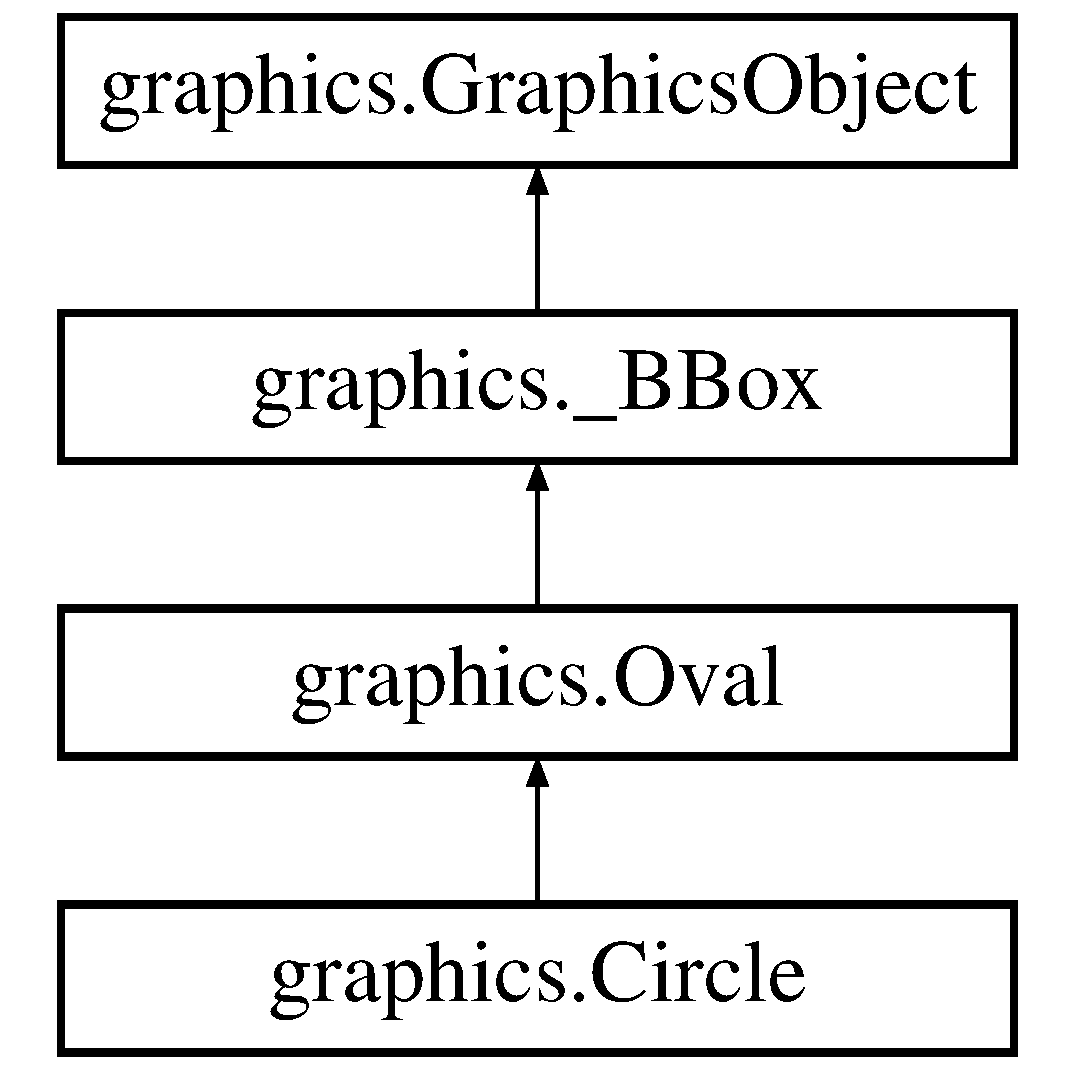
\includegraphics[height=4.000000cm]{classgraphics_1_1_circle}
\end{center}
\end{figure}
\subsection*{Public Member Functions}
\begin{DoxyCompactItemize}
\item 
def {\bfseries \+\_\+\+\_\+init\+\_\+\+\_\+} (self, center, radius)\hypertarget{classgraphics_1_1_circle_adf9ab62e2d952cf52cfecba9acfd5660}{}\label{classgraphics_1_1_circle_adf9ab62e2d952cf52cfecba9acfd5660}

\item 
def {\bfseries \+\_\+\+\_\+repr\+\_\+\+\_\+} (self)\hypertarget{classgraphics_1_1_circle_a7acb1acc63613799ff2724cb05d75750}{}\label{classgraphics_1_1_circle_a7acb1acc63613799ff2724cb05d75750}

\item 
def {\bfseries clone} (self)\hypertarget{classgraphics_1_1_circle_ae575b71c63ce889e4c872c792d748f7b}{}\label{classgraphics_1_1_circle_ae575b71c63ce889e4c872c792d748f7b}

\item 
def {\bfseries get\+Radius} (self)\hypertarget{classgraphics_1_1_circle_a420b2e69c4d116c094dc6bd6b1e81839}{}\label{classgraphics_1_1_circle_a420b2e69c4d116c094dc6bd6b1e81839}

\end{DoxyCompactItemize}
\subsection*{Public Attributes}
\begin{DoxyCompactItemize}
\item 
{\bfseries radius}\hypertarget{classgraphics_1_1_circle_aacc54bd0a94edd646405c8718cbeb47c}{}\label{classgraphics_1_1_circle_aacc54bd0a94edd646405c8718cbeb47c}

\end{DoxyCompactItemize}


The documentation for this class was generated from the following file\+:\begin{DoxyCompactItemize}
\item 
graphics.\+py\end{DoxyCompactItemize}

\hypertarget{class_parsing_classes_actual_1_1_cout_statement}{}\section{Parsing\+Classes\+Actual.\+Cout\+Statement Class Reference}
\label{class_parsing_classes_actual_1_1_cout_statement}\index{Parsing\+Classes\+Actual.\+Cout\+Statement@{Parsing\+Classes\+Actual.\+Cout\+Statement}}


class for cout statement  


\subsection*{Public Member Functions}
\begin{DoxyCompactItemize}
\item 
def \hyperlink{class_parsing_classes_actual_1_1_cout_statement_a0e4930ecbd6e69aac9830659965c4c9c}{\+\_\+\+\_\+init\+\_\+\+\_\+} (self, list\+Of\+Express, snippet)
\begin{DoxyCompactList}\small\item\em the constructor \end{DoxyCompactList}\item 
def \hyperlink{class_parsing_classes_actual_1_1_cout_statement_ad0afd27df037b3f14e777a1f3fa4173e}{exec} (self)\hypertarget{class_parsing_classes_actual_1_1_cout_statement_ad0afd27df037b3f14e777a1f3fa4173e}{}\label{class_parsing_classes_actual_1_1_cout_statement_ad0afd27df037b3f14e777a1f3fa4173e}

\begin{DoxyCompactList}\small\item\em The executable which prints the evaluated expressions. \end{DoxyCompactList}\end{DoxyCompactItemize}
\subsection*{Public Attributes}
\begin{DoxyCompactItemize}
\item 
{\bfseries list\+Of\+Express}\hypertarget{class_parsing_classes_actual_1_1_cout_statement_a7d1d563940af735f9155788a3806edeb}{}\label{class_parsing_classes_actual_1_1_cout_statement_a7d1d563940af735f9155788a3806edeb}

\item 
{\bfseries snippet}\hypertarget{class_parsing_classes_actual_1_1_cout_statement_a6cbedbd0181ff15b696b8a8a6c9e4ef2}{}\label{class_parsing_classes_actual_1_1_cout_statement_a6cbedbd0181ff15b696b8a8a6c9e4ef2}

\end{DoxyCompactItemize}


\subsection{Detailed Description}
class for cout statement 

\subsection{Constructor \& Destructor Documentation}
\index{Parsing\+Classes\+Actual\+::\+Cout\+Statement@{Parsing\+Classes\+Actual\+::\+Cout\+Statement}!\+\_\+\+\_\+init\+\_\+\+\_\+@{\+\_\+\+\_\+init\+\_\+\+\_\+}}
\index{\+\_\+\+\_\+init\+\_\+\+\_\+@{\+\_\+\+\_\+init\+\_\+\+\_\+}!Parsing\+Classes\+Actual\+::\+Cout\+Statement@{Parsing\+Classes\+Actual\+::\+Cout\+Statement}}
\subsubsection[{\texorpdfstring{\+\_\+\+\_\+init\+\_\+\+\_\+(self, list\+Of\+Express, snippet)}{__init__(self, listOfExpress, snippet)}}]{\setlength{\rightskip}{0pt plus 5cm}def Parsing\+Classes\+Actual.\+Cout\+Statement.\+\_\+\+\_\+init\+\_\+\+\_\+ (
\begin{DoxyParamCaption}
\item[{}]{self, }
\item[{}]{list\+Of\+Express, }
\item[{}]{snippet}
\end{DoxyParamCaption}
)}\hypertarget{class_parsing_classes_actual_1_1_cout_statement_a0e4930ecbd6e69aac9830659965c4c9c}{}\label{class_parsing_classes_actual_1_1_cout_statement_a0e4930ecbd6e69aac9830659965c4c9c}


the constructor 


\begin{DoxyParams}{Parameters}
{\em list\+Of\+Express} & The expressions that have to be printed \\
\hline
{\em snippet} & The relevant code snippet \\
\hline
\end{DoxyParams}


The documentation for this class was generated from the following file\+:\begin{DoxyCompactItemize}
\item 
Parsing\+Classes\+Actual.\+py\end{DoxyCompactItemize}

\hypertarget{classparser_classes_1_1_cout_statement}{}\section{parser\+Classes.\+Cout\+Statement Class Reference}
\label{classparser_classes_1_1_cout_statement}\index{parser\+Classes.\+Cout\+Statement@{parser\+Classes.\+Cout\+Statement}}
\subsection*{Public Member Functions}
\begin{DoxyCompactItemize}
\item 
def {\bfseries \+\_\+\+\_\+init\+\_\+\+\_\+} (self, list\+Of\+Express)\hypertarget{classparser_classes_1_1_cout_statement_ad06ead1f60e93546e7445ce5d0219504}{}\label{classparser_classes_1_1_cout_statement_ad06ead1f60e93546e7445ce5d0219504}

\item 
def {\bfseries exec} (self)\hypertarget{classparser_classes_1_1_cout_statement_a8a94c5c6abe84a07b91e3558a39fa640}{}\label{classparser_classes_1_1_cout_statement_a8a94c5c6abe84a07b91e3558a39fa640}

\end{DoxyCompactItemize}
\subsection*{Public Attributes}
\begin{DoxyCompactItemize}
\item 
{\bfseries list\+Of\+Express}\hypertarget{classparser_classes_1_1_cout_statement_a07537d9231860bf00d245bcca3766986}{}\label{classparser_classes_1_1_cout_statement_a07537d9231860bf00d245bcca3766986}

\end{DoxyCompactItemize}


The documentation for this class was generated from the following file\+:\begin{DoxyCompactItemize}
\item 
parser\+Classes.\+py\end{DoxyCompactItemize}

\hypertarget{class_parsing_classes_actual_1_1_data_structure_declaration}{}\section{Parsing\+Classes\+Actual.\+Data\+Structure\+Declaration Class Reference}
\label{class_parsing_classes_actual_1_1_data_structure_declaration}\index{Parsing\+Classes\+Actual.\+Data\+Structure\+Declaration@{Parsing\+Classes\+Actual.\+Data\+Structure\+Declaration}}


initialization for our data structures  


\subsection*{Public Member Functions}
\begin{DoxyCompactItemize}
\item 
def \hyperlink{class_parsing_classes_actual_1_1_data_structure_declaration_aa30264067a870240581f89487ee4834c}{\+\_\+\+\_\+init\+\_\+\+\_\+} (self, class\+Name, name, vartype, snippet)
\begin{DoxyCompactList}\small\item\em The constructor. \end{DoxyCompactList}\item 
def \hyperlink{class_parsing_classes_actual_1_1_data_structure_declaration_a69e6e4ab0c53bd579815a03bd333c88c}{exec} (self)\hypertarget{class_parsing_classes_actual_1_1_data_structure_declaration_a69e6e4ab0c53bd579815a03bd333c88c}{}\label{class_parsing_classes_actual_1_1_data_structure_declaration_a69e6e4ab0c53bd579815a03bd333c88c}

\begin{DoxyCompactList}\small\item\em The executable function. \end{DoxyCompactList}\end{DoxyCompactItemize}
\subsection*{Public Attributes}
\begin{DoxyCompactItemize}
\item 
{\bfseries name}\hypertarget{class_parsing_classes_actual_1_1_data_structure_declaration_ac8db5fc9818883f97ab6d2fd2671be03}{}\label{class_parsing_classes_actual_1_1_data_structure_declaration_ac8db5fc9818883f97ab6d2fd2671be03}

\item 
{\bfseries vartype}\hypertarget{class_parsing_classes_actual_1_1_data_structure_declaration_ae97cc741ab55e0998ef6b70dec8e5576}{}\label{class_parsing_classes_actual_1_1_data_structure_declaration_ae97cc741ab55e0998ef6b70dec8e5576}

\item 
{\bfseries the\+Class}\hypertarget{class_parsing_classes_actual_1_1_data_structure_declaration_a1955dd224837df313ca02bc67d22327d}{}\label{class_parsing_classes_actual_1_1_data_structure_declaration_a1955dd224837df313ca02bc67d22327d}

\item 
{\bfseries snippet}\hypertarget{class_parsing_classes_actual_1_1_data_structure_declaration_aef73b24e2d4216905f4cffca0ce6f002}{}\label{class_parsing_classes_actual_1_1_data_structure_declaration_aef73b24e2d4216905f4cffca0ce6f002}

\end{DoxyCompactItemize}


\subsection{Detailed Description}
initialization for our data structures 

\subsection{Constructor \& Destructor Documentation}
\index{Parsing\+Classes\+Actual\+::\+Data\+Structure\+Declaration@{Parsing\+Classes\+Actual\+::\+Data\+Structure\+Declaration}!\+\_\+\+\_\+init\+\_\+\+\_\+@{\+\_\+\+\_\+init\+\_\+\+\_\+}}
\index{\+\_\+\+\_\+init\+\_\+\+\_\+@{\+\_\+\+\_\+init\+\_\+\+\_\+}!Parsing\+Classes\+Actual\+::\+Data\+Structure\+Declaration@{Parsing\+Classes\+Actual\+::\+Data\+Structure\+Declaration}}
\subsubsection[{\texorpdfstring{\+\_\+\+\_\+init\+\_\+\+\_\+(self, class\+Name, name, vartype, snippet)}{__init__(self, className, name, vartype, snippet)}}]{\setlength{\rightskip}{0pt plus 5cm}def Parsing\+Classes\+Actual.\+Data\+Structure\+Declaration.\+\_\+\+\_\+init\+\_\+\+\_\+ (
\begin{DoxyParamCaption}
\item[{}]{self, }
\item[{}]{class\+Name, }
\item[{}]{name, }
\item[{}]{vartype, }
\item[{}]{snippet}
\end{DoxyParamCaption}
)}\hypertarget{class_parsing_classes_actual_1_1_data_structure_declaration_aa30264067a870240581f89487ee4834c}{}\label{class_parsing_classes_actual_1_1_data_structure_declaration_aa30264067a870240581f89487ee4834c}


The constructor. 


\begin{DoxyParams}{Parameters}
{\em class\+Name} & The name of datatype to be initialized \\
\hline
{\em name} & The name of datatype variable \\
\hline
{\em vartype} & The type of data which is stored in this datatype \\
\hline
{\em snippet} & The relevant code snippet \\
\hline
\end{DoxyParams}


The documentation for this class was generated from the following file\+:\begin{DoxyCompactItemize}
\item 
Parsing\+Classes\+Actual.\+py\end{DoxyCompactItemize}

\hypertarget{classparser_classes_1_1_data_structure_declaration}{}\section{parser\+Classes.\+Data\+Structure\+Declaration Class Reference}
\label{classparser_classes_1_1_data_structure_declaration}\index{parser\+Classes.\+Data\+Structure\+Declaration@{parser\+Classes.\+Data\+Structure\+Declaration}}
\subsection*{Public Member Functions}
\begin{DoxyCompactItemize}
\item 
def {\bfseries \+\_\+\+\_\+init\+\_\+\+\_\+} (self, class\+Name, name, vartype)\hypertarget{classparser_classes_1_1_data_structure_declaration_abf31307e4d0cb3dadb9309182def6a2b}{}\label{classparser_classes_1_1_data_structure_declaration_abf31307e4d0cb3dadb9309182def6a2b}

\item 
def {\bfseries exec} (self)\hypertarget{classparser_classes_1_1_data_structure_declaration_ab2fa0b82dbfc8fc1cfc49ba21bf02977}{}\label{classparser_classes_1_1_data_structure_declaration_ab2fa0b82dbfc8fc1cfc49ba21bf02977}

\end{DoxyCompactItemize}
\subsection*{Public Attributes}
\begin{DoxyCompactItemize}
\item 
{\bfseries name}\hypertarget{classparser_classes_1_1_data_structure_declaration_a72028991597dde706393f738e06687a2}{}\label{classparser_classes_1_1_data_structure_declaration_a72028991597dde706393f738e06687a2}

\item 
{\bfseries vartype}\hypertarget{classparser_classes_1_1_data_structure_declaration_adfc5633b6c9fb8292f8c9e59b2c2ab2d}{}\label{classparser_classes_1_1_data_structure_declaration_adfc5633b6c9fb8292f8c9e59b2c2ab2d}

\item 
{\bfseries the\+Class}\hypertarget{classparser_classes_1_1_data_structure_declaration_abfaff3bb31319c434bb7c37702dd2a93}{}\label{classparser_classes_1_1_data_structure_declaration_abfaff3bb31319c434bb7c37702dd2a93}

\end{DoxyCompactItemize}


The documentation for this class was generated from the following file\+:\begin{DoxyCompactItemize}
\item 
parser\+Classes.\+py\end{DoxyCompactItemize}

\hypertarget{classgraphics_1_1_entry}{}\section{graphics.\+Entry Class Reference}
\label{classgraphics_1_1_entry}\index{graphics.\+Entry@{graphics.\+Entry}}
Inheritance diagram for graphics.\+Entry\+:\begin{figure}[H]
\begin{center}
\leavevmode
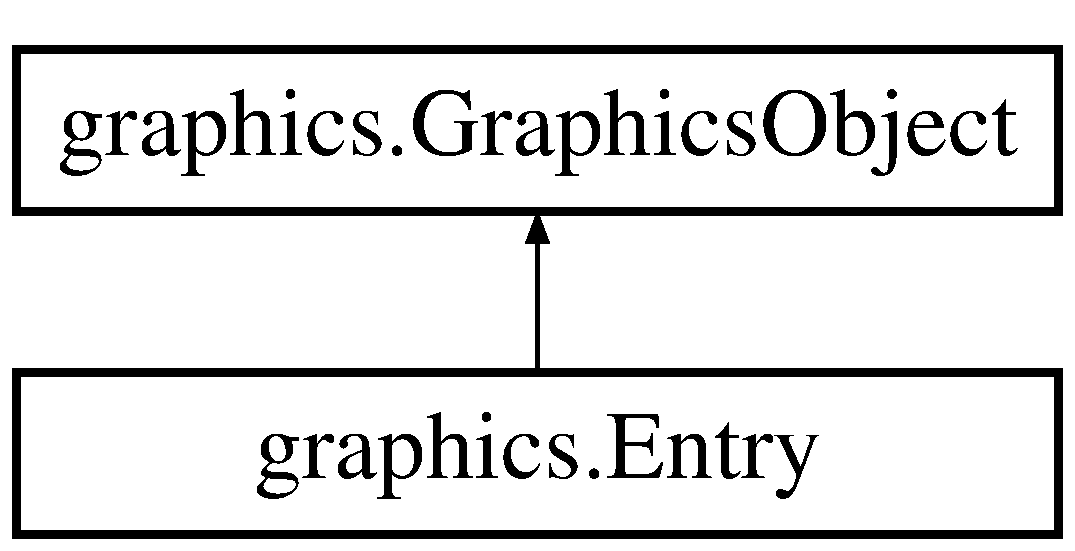
\includegraphics[height=2.000000cm]{classgraphics_1_1_entry}
\end{center}
\end{figure}
\subsection*{Public Member Functions}
\begin{DoxyCompactItemize}
\item 
\mbox{\Hypertarget{classgraphics_1_1_entry_afb968169b4da90b66fd7cc34ffe8d93a}\label{classgraphics_1_1_entry_afb968169b4da90b66fd7cc34ffe8d93a}} 
def {\bfseries \+\_\+\+\_\+init\+\_\+\+\_\+} (self, p, width)
\item 
\mbox{\Hypertarget{classgraphics_1_1_entry_aea5b15bc4da7ede46e7cdd9991748c9e}\label{classgraphics_1_1_entry_aea5b15bc4da7ede46e7cdd9991748c9e}} 
def {\bfseries \+\_\+\+\_\+repr\+\_\+\+\_\+} (self)
\item 
\mbox{\Hypertarget{classgraphics_1_1_entry_a0a09f97f04f3d54bf8a5ca3edf99ef19}\label{classgraphics_1_1_entry_a0a09f97f04f3d54bf8a5ca3edf99ef19}} 
def {\bfseries get\+Text} (self)
\item 
\mbox{\Hypertarget{classgraphics_1_1_entry_ab0a6e815195a49e1e682eb94d4735c9e}\label{classgraphics_1_1_entry_ab0a6e815195a49e1e682eb94d4735c9e}} 
def {\bfseries get\+Anchor} (self)
\item 
\mbox{\Hypertarget{classgraphics_1_1_entry_a15f95f96006286fead5e136792932434}\label{classgraphics_1_1_entry_a15f95f96006286fead5e136792932434}} 
def {\bfseries clone} (self)
\item 
\mbox{\Hypertarget{classgraphics_1_1_entry_a6a8f8c6cbc38f8efabe66785f09c735c}\label{classgraphics_1_1_entry_a6a8f8c6cbc38f8efabe66785f09c735c}} 
def {\bfseries set\+Text} (self, t)
\item 
\mbox{\Hypertarget{classgraphics_1_1_entry_ad1d04de2ffd36b0b6d6733fe992303ee}\label{classgraphics_1_1_entry_ad1d04de2ffd36b0b6d6733fe992303ee}} 
def {\bfseries set\+Fill} (self, color)
\item 
\mbox{\Hypertarget{classgraphics_1_1_entry_abaaf60215354bfbcecbd506e7176d54b}\label{classgraphics_1_1_entry_abaaf60215354bfbcecbd506e7176d54b}} 
def {\bfseries set\+Face} (self, face)
\item 
\mbox{\Hypertarget{classgraphics_1_1_entry_a0e4a339c1fa89e228f750b7d5c6d8ced}\label{classgraphics_1_1_entry_a0e4a339c1fa89e228f750b7d5c6d8ced}} 
def {\bfseries set\+Size} (self, size)
\item 
\mbox{\Hypertarget{classgraphics_1_1_entry_aa36a5f9e71331b921f0728c25631d9c3}\label{classgraphics_1_1_entry_aa36a5f9e71331b921f0728c25631d9c3}} 
def {\bfseries set\+Style} (self, style)
\item 
\mbox{\Hypertarget{classgraphics_1_1_entry_a44e4c12f4ec190351fc8dc29bf7f0a37}\label{classgraphics_1_1_entry_a44e4c12f4ec190351fc8dc29bf7f0a37}} 
def {\bfseries set\+Text\+Color} (self, color)
\end{DoxyCompactItemize}
\subsection*{Public Attributes}
\begin{DoxyCompactItemize}
\item 
\mbox{\Hypertarget{classgraphics_1_1_entry_a80e7267b0c2117459d13532c253e608f}\label{classgraphics_1_1_entry_a80e7267b0c2117459d13532c253e608f}} 
{\bfseries anchor}
\item 
\mbox{\Hypertarget{classgraphics_1_1_entry_a3c71a6cb1110ae9da3edef095fbb61e5}\label{classgraphics_1_1_entry_a3c71a6cb1110ae9da3edef095fbb61e5}} 
{\bfseries width}
\item 
\mbox{\Hypertarget{classgraphics_1_1_entry_ad606e7fd6c89a56ffd6c35385bc050e6}\label{classgraphics_1_1_entry_ad606e7fd6c89a56ffd6c35385bc050e6}} 
{\bfseries text}
\item 
\mbox{\Hypertarget{classgraphics_1_1_entry_aaa0a15f51427af10dd5adc7e0aa3d553}\label{classgraphics_1_1_entry_aaa0a15f51427af10dd5adc7e0aa3d553}} 
{\bfseries fill}
\item 
\mbox{\Hypertarget{classgraphics_1_1_entry_a96d564c2ac5f5bc21e6353f7b6e702c1}\label{classgraphics_1_1_entry_a96d564c2ac5f5bc21e6353f7b6e702c1}} 
{\bfseries color}
\item 
\mbox{\Hypertarget{classgraphics_1_1_entry_a03940868372e90882d320d9a402dec14}\label{classgraphics_1_1_entry_a03940868372e90882d320d9a402dec14}} 
{\bfseries font}
\item 
\mbox{\Hypertarget{classgraphics_1_1_entry_a344bdacc19d9c10e355e21357a94c38d}\label{classgraphics_1_1_entry_a344bdacc19d9c10e355e21357a94c38d}} 
{\bfseries entry}
\end{DoxyCompactItemize}


The documentation for this class was generated from the following file\+:\begin{DoxyCompactItemize}
\item 
graphics.\+py\end{DoxyCompactItemize}

\hypertarget{classexecution_stack_1_1_execution_stack}{}\section{execution\+Stack.\+Execution\+Stack Class Reference}
\label{classexecution_stack_1_1_execution_stack}\index{execution\+Stack.\+Execution\+Stack@{execution\+Stack.\+Execution\+Stack}}
\subsection*{Public Member Functions}
\begin{DoxyCompactItemize}
\item 
def {\bfseries \+\_\+\+\_\+init\+\_\+\+\_\+} (self)\hypertarget{classexecution_stack_1_1_execution_stack_a955ae5d9778e86b1c0325a0873fad686}{}\label{classexecution_stack_1_1_execution_stack_a955ae5d9778e86b1c0325a0873fad686}

\item 
def {\bfseries push} (self, dictionary)\hypertarget{classexecution_stack_1_1_execution_stack_a228350aa77b6029b1aafdcd34612ce61}{}\label{classexecution_stack_1_1_execution_stack_a228350aa77b6029b1aafdcd34612ce61}

\item 
def {\bfseries add\+Data} (self, key, val)\hypertarget{classexecution_stack_1_1_execution_stack_a7df2cbd7895c11c301631b45d7d24e1b}{}\label{classexecution_stack_1_1_execution_stack_a7df2cbd7895c11c301631b45d7d24e1b}

\item 
def {\bfseries modify\+Data} (self, key, val, index)\hypertarget{classexecution_stack_1_1_execution_stack_ab1bcc59b2d0f26c0178f7c457efce474}{}\label{classexecution_stack_1_1_execution_stack_ab1bcc59b2d0f26c0178f7c457efce474}

\item 
def {\bfseries delete\+Data} (self, key, index)\hypertarget{classexecution_stack_1_1_execution_stack_aaa0f483291031cc81423a4525838f8d0}{}\label{classexecution_stack_1_1_execution_stack_aaa0f483291031cc81423a4525838f8d0}

\item 
def {\bfseries pop} (self)\hypertarget{classexecution_stack_1_1_execution_stack_aec0e4c8c421162e42668372c1309e6c5}{}\label{classexecution_stack_1_1_execution_stack_aec0e4c8c421162e42668372c1309e6c5}

\end{DoxyCompactItemize}
\subsection*{Public Attributes}
\begin{DoxyCompactItemize}
\item 
{\bfseries head}\hypertarget{classexecution_stack_1_1_execution_stack_ad712e443c44369cb1de23bb4010c89f3}{}\label{classexecution_stack_1_1_execution_stack_ad712e443c44369cb1de23bb4010c89f3}

\item 
{\bfseries size}\hypertarget{classexecution_stack_1_1_execution_stack_a7011596156e1e3128bb44099347b5db8}{}\label{classexecution_stack_1_1_execution_stack_a7011596156e1e3128bb44099347b5db8}

\end{DoxyCompactItemize}


The documentation for this class was generated from the following file\+:\begin{DoxyCompactItemize}
\item 
execution\+Stack.\+py\end{DoxyCompactItemize}

\hypertarget{class_parsing_classes_actual_1_1_expression}{}\section{Parsing\+Classes\+Actual.\+Expression Class Reference}
\label{class_parsing_classes_actual_1_1_expression}\index{Parsing\+Classes\+Actual.\+Expression@{Parsing\+Classes\+Actual.\+Expression}}
\subsection*{Public Member Functions}
\begin{DoxyCompactItemize}
\item 
\mbox{\Hypertarget{class_parsing_classes_actual_1_1_expression_a76e27ac0110d45f2943ed2a48b0ec379}\label{class_parsing_classes_actual_1_1_expression_a76e27ac0110d45f2943ed2a48b0ec379}} 
def {\bfseries \+\_\+\+\_\+init\+\_\+\+\_\+} (self)
\item 
\mbox{\Hypertarget{class_parsing_classes_actual_1_1_expression_acfc7f3fdfc30916c3684f29994c51e53}\label{class_parsing_classes_actual_1_1_expression_acfc7f3fdfc30916c3684f29994c51e53}} 
def {\bfseries add\+Element} (self, element)
\item 
\mbox{\Hypertarget{class_parsing_classes_actual_1_1_expression_a3a22e0b9d00beb8eb7fa40cfb45db6ed}\label{class_parsing_classes_actual_1_1_expression_a3a22e0b9d00beb8eb7fa40cfb45db6ed}} 
def {\bfseries eval} (self)
\end{DoxyCompactItemize}
\subsection*{Public Attributes}
\begin{DoxyCompactItemize}
\item 
\mbox{\Hypertarget{class_parsing_classes_actual_1_1_expression_a41891da0f782b121512065f8bbcf7c1b}\label{class_parsing_classes_actual_1_1_expression_a41891da0f782b121512065f8bbcf7c1b}} 
{\bfseries elements}
\end{DoxyCompactItemize}


The documentation for this class was generated from the following file\+:\begin{DoxyCompactItemize}
\item 
Parsing\+Classes\+Actual.\+py\end{DoxyCompactItemize}

\hypertarget{classparser_classes_1_1_expression}{}\section{parser\+Classes.\+Expression Class Reference}
\label{classparser_classes_1_1_expression}\index{parser\+Classes.\+Expression@{parser\+Classes.\+Expression}}
\subsection*{Public Member Functions}
\begin{DoxyCompactItemize}
\item 
def {\bfseries \+\_\+\+\_\+init\+\_\+\+\_\+} (self)\hypertarget{classparser_classes_1_1_expression_ae01f3aaff0913d71e84dd96fb520541c}{}\label{classparser_classes_1_1_expression_ae01f3aaff0913d71e84dd96fb520541c}

\item 
def {\bfseries add\+Element} (self, element)\hypertarget{classparser_classes_1_1_expression_a0065ec38485063fce29c52fcd4fa0156}{}\label{classparser_classes_1_1_expression_a0065ec38485063fce29c52fcd4fa0156}

\item 
def {\bfseries eval} (self)\hypertarget{classparser_classes_1_1_expression_a9eb95e98f5d2ac1c133830abf80dae82}{}\label{classparser_classes_1_1_expression_a9eb95e98f5d2ac1c133830abf80dae82}

\end{DoxyCompactItemize}
\subsection*{Public Attributes}
\begin{DoxyCompactItemize}
\item 
{\bfseries elements}\hypertarget{classparser_classes_1_1_expression_a68033b9f9c015d5507c42206c801e324}{}\label{classparser_classes_1_1_expression_a68033b9f9c015d5507c42206c801e324}

\end{DoxyCompactItemize}


The documentation for this class was generated from the following file\+:\begin{DoxyCompactItemize}
\item 
parser\+Classes.\+py\end{DoxyCompactItemize}

\hypertarget{class_parsing_classes_actual_1_1_factor}{}\section{Parsing\+Classes\+Actual.\+Factor Class Reference}
\label{class_parsing_classes_actual_1_1_factor}\index{Parsing\+Classes\+Actual.\+Factor@{Parsing\+Classes\+Actual.\+Factor}}
\subsection*{Public Member Functions}
\begin{DoxyCompactItemize}
\item 
\mbox{\Hypertarget{class_parsing_classes_actual_1_1_factor_ad0bf99ed1dc466e9994adbca9f507d55}\label{class_parsing_classes_actual_1_1_factor_ad0bf99ed1dc466e9994adbca9f507d55}} 
def {\bfseries \+\_\+\+\_\+init\+\_\+\+\_\+} (self)
\item 
\mbox{\Hypertarget{class_parsing_classes_actual_1_1_factor_a6dfb419731bf782dd7361c66a783df0d}\label{class_parsing_classes_actual_1_1_factor_a6dfb419731bf782dd7361c66a783df0d}} 
def {\bfseries add\+Element} (self, element)
\item 
\mbox{\Hypertarget{class_parsing_classes_actual_1_1_factor_a7c0779ac99786001a11b9a0ae6db5896}\label{class_parsing_classes_actual_1_1_factor_a7c0779ac99786001a11b9a0ae6db5896}} 
def {\bfseries eval} (self)
\end{DoxyCompactItemize}
\subsection*{Public Attributes}
\begin{DoxyCompactItemize}
\item 
\mbox{\Hypertarget{class_parsing_classes_actual_1_1_factor_a0e252f30c9cc0e8016d765a1ee7028b4}\label{class_parsing_classes_actual_1_1_factor_a0e252f30c9cc0e8016d765a1ee7028b4}} 
{\bfseries elements}
\end{DoxyCompactItemize}


The documentation for this class was generated from the following file\+:\begin{DoxyCompactItemize}
\item 
Parsing\+Classes\+Actual.\+py\end{DoxyCompactItemize}

\hypertarget{classparser_classes_1_1_factor}{}\section{parser\+Classes.\+Factor Class Reference}
\label{classparser_classes_1_1_factor}\index{parser\+Classes.\+Factor@{parser\+Classes.\+Factor}}
\subsection*{Public Member Functions}
\begin{DoxyCompactItemize}
\item 
def {\bfseries \+\_\+\+\_\+init\+\_\+\+\_\+} (self)\hypertarget{classparser_classes_1_1_factor_a50cc8e66fcea86b531bc0e490ded63f2}{}\label{classparser_classes_1_1_factor_a50cc8e66fcea86b531bc0e490ded63f2}

\item 
def {\bfseries add\+Element} (self, element)\hypertarget{classparser_classes_1_1_factor_ad5d74ecd0f9ea5bf50e375cda5f57964}{}\label{classparser_classes_1_1_factor_ad5d74ecd0f9ea5bf50e375cda5f57964}

\item 
def {\bfseries eval} (self)\hypertarget{classparser_classes_1_1_factor_a5d9064846ca5c7367ab0b0bcfb200774}{}\label{classparser_classes_1_1_factor_a5d9064846ca5c7367ab0b0bcfb200774}

\end{DoxyCompactItemize}
\subsection*{Public Attributes}
\begin{DoxyCompactItemize}
\item 
{\bfseries elements}\hypertarget{classparser_classes_1_1_factor_ad5f90e3a7a1ebaa63f456d499e4d05f5}{}\label{classparser_classes_1_1_factor_ad5f90e3a7a1ebaa63f456d499e4d05f5}

\end{DoxyCompactItemize}


The documentation for this class was generated from the following file\+:\begin{DoxyCompactItemize}
\item 
parser\+Classes.\+py\end{DoxyCompactItemize}

\hypertarget{classparser_classes_1_1_float}{}\section{parser\+Classes.\+Float Class Reference}
\label{classparser_classes_1_1_float}\index{parser\+Classes.\+Float@{parser\+Classes.\+Float}}
Inheritance diagram for parser\+Classes.\+Float\+:\begin{figure}[H]
\begin{center}
\leavevmode
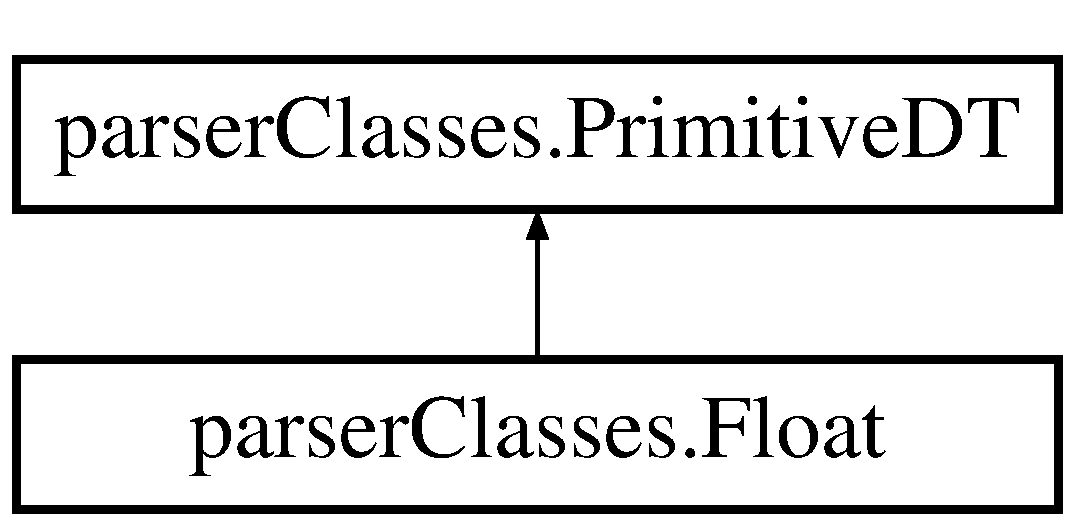
\includegraphics[height=2.000000cm]{classparser_classes_1_1_float}
\end{center}
\end{figure}
\subsection*{Public Member Functions}
\begin{DoxyCompactItemize}
\item 
\mbox{\Hypertarget{classparser_classes_1_1_float_a6b381bc911c79a2e93df1627ca2267df}\label{classparser_classes_1_1_float_a6b381bc911c79a2e93df1627ca2267df}} 
def {\bfseries \+\_\+\+\_\+init\+\_\+\+\_\+} (self, value=0.\+0)
\item 
\mbox{\Hypertarget{classparser_classes_1_1_float_a5570384fde83d172e3fe1b176be8521e}\label{classparser_classes_1_1_float_a5570384fde83d172e3fe1b176be8521e}} 
def {\bfseries give\+Type} (self)
\item 
\mbox{\Hypertarget{classparser_classes_1_1_float_a825903e0f131e7169e28fab644c26344}\label{classparser_classes_1_1_float_a825903e0f131e7169e28fab644c26344}} 
def {\bfseries update} (self, val)
\end{DoxyCompactItemize}
\subsection*{Public Attributes}
\begin{DoxyCompactItemize}
\item 
\mbox{\Hypertarget{classparser_classes_1_1_float_abb886ca1c6bbaa84a9b08d57db80b4c7}\label{classparser_classes_1_1_float_abb886ca1c6bbaa84a9b08d57db80b4c7}} 
{\bfseries value}
\end{DoxyCompactItemize}


The documentation for this class was generated from the following file\+:\begin{DoxyCompactItemize}
\item 
parser\+Classes.\+py\end{DoxyCompactItemize}

\hypertarget{class_parsing_classes_actual_1_1_float}{}\section{Parsing\+Classes\+Actual.\+Float Class Reference}
\label{class_parsing_classes_actual_1_1_float}\index{Parsing\+Classes\+Actual.\+Float@{Parsing\+Classes\+Actual.\+Float}}


class for float datatype  


Inheritance diagram for Parsing\+Classes\+Actual.\+Float\+:\begin{figure}[H]
\begin{center}
\leavevmode
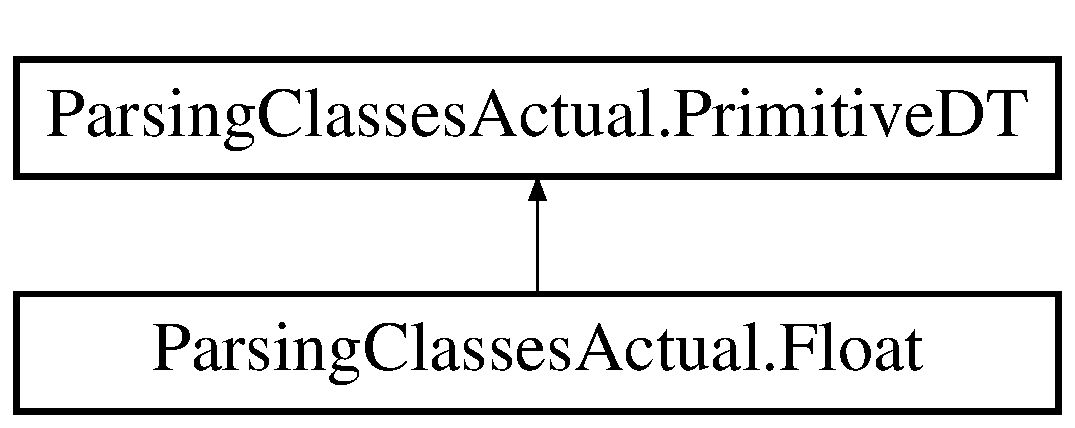
\includegraphics[height=2.000000cm]{class_parsing_classes_actual_1_1_float}
\end{center}
\end{figure}
\subsection*{Public Member Functions}
\begin{DoxyCompactItemize}
\item 
def \hyperlink{class_parsing_classes_actual_1_1_float_a285387447fcf577d0ef3b1f3f8f4e69b}{\+\_\+\+\_\+init\+\_\+\+\_\+} (self, value=0.\+0)
\begin{DoxyCompactList}\small\item\em the constructor \end{DoxyCompactList}\item 
def \hyperlink{class_parsing_classes_actual_1_1_float_ae424695b61f25088e1378a672da9036c}{give\+Type} (self)\hypertarget{class_parsing_classes_actual_1_1_float_ae424695b61f25088e1378a672da9036c}{}\label{class_parsing_classes_actual_1_1_float_ae424695b61f25088e1378a672da9036c}

\begin{DoxyCompactList}\small\item\em returns the type of value \end{DoxyCompactList}\item 
def \hyperlink{class_parsing_classes_actual_1_1_float_a87739feda988d226bb1e384b31cbc113}{update} (self, val)\hypertarget{class_parsing_classes_actual_1_1_float_a87739feda988d226bb1e384b31cbc113}{}\label{class_parsing_classes_actual_1_1_float_a87739feda988d226bb1e384b31cbc113}

\begin{DoxyCompactList}\small\item\em updates the stored value by typecasting it \end{DoxyCompactList}\end{DoxyCompactItemize}
\subsection*{Public Attributes}
\begin{DoxyCompactItemize}
\item 
{\bfseries value}\hypertarget{class_parsing_classes_actual_1_1_float_ad209bb476885a17b23cc2a54646794a3}{}\label{class_parsing_classes_actual_1_1_float_ad209bb476885a17b23cc2a54646794a3}

\end{DoxyCompactItemize}


\subsection{Detailed Description}
class for float datatype 

\subsection{Constructor \& Destructor Documentation}
\index{Parsing\+Classes\+Actual\+::\+Float@{Parsing\+Classes\+Actual\+::\+Float}!\+\_\+\+\_\+init\+\_\+\+\_\+@{\+\_\+\+\_\+init\+\_\+\+\_\+}}
\index{\+\_\+\+\_\+init\+\_\+\+\_\+@{\+\_\+\+\_\+init\+\_\+\+\_\+}!Parsing\+Classes\+Actual\+::\+Float@{Parsing\+Classes\+Actual\+::\+Float}}
\subsubsection[{\texorpdfstring{\+\_\+\+\_\+init\+\_\+\+\_\+(self, value=0.\+0)}{__init__(self, value=0.0)}}]{\setlength{\rightskip}{0pt plus 5cm}def Parsing\+Classes\+Actual.\+Float.\+\_\+\+\_\+init\+\_\+\+\_\+ (
\begin{DoxyParamCaption}
\item[{}]{self, }
\item[{}]{value = {\ttfamily 0.0}}
\end{DoxyParamCaption}
)}\hypertarget{class_parsing_classes_actual_1_1_float_a285387447fcf577d0ef3b1f3f8f4e69b}{}\label{class_parsing_classes_actual_1_1_float_a285387447fcf577d0ef3b1f3f8f4e69b}


the constructor 


\begin{DoxyParams}{Parameters}
{\em the} & value of datatype \\
\hline
\end{DoxyParams}


The documentation for this class was generated from the following file\+:\begin{DoxyCompactItemize}
\item 
Parsing\+Classes\+Actual.\+py\end{DoxyCompactItemize}

\hypertarget{class_parsing_classes_actual_1_1_for_loop}{}\section{Parsing\+Classes\+Actual.\+For\+Loop Class Reference}
\label{class_parsing_classes_actual_1_1_for_loop}\index{Parsing\+Classes\+Actual.\+For\+Loop@{Parsing\+Classes\+Actual.\+For\+Loop}}


the class for for-\/loop containing declaration,conditions,block and updation  


\subsection*{Public Member Functions}
\begin{DoxyCompactItemize}
\item 
def \hyperlink{class_parsing_classes_actual_1_1_for_loop_a1a97fc2d259b140ef8db3d3d455a286f}{\+\_\+\+\_\+init\+\_\+\+\_\+} (self, declare, express, assign, statement\+List, snippet)
\begin{DoxyCompactList}\small\item\em the constructor \end{DoxyCompactList}\item 
def \hyperlink{class_parsing_classes_actual_1_1_for_loop_a817cdfbfca1b14eb973d203863292940}{exec} (self)\hypertarget{class_parsing_classes_actual_1_1_for_loop_a817cdfbfca1b14eb973d203863292940}{}\label{class_parsing_classes_actual_1_1_for_loop_a817cdfbfca1b14eb973d203863292940}

\begin{DoxyCompactList}\small\item\em The executable which implements the \hyperlink{class_parsing_classes_actual_1_1_for_loop}{For\+Loop} in correct order. \end{DoxyCompactList}\end{DoxyCompactItemize}
\subsection*{Public Attributes}
\begin{DoxyCompactItemize}
\item 
{\bfseries declare}\hypertarget{class_parsing_classes_actual_1_1_for_loop_a550adc5c22fce87be47a83598843c706}{}\label{class_parsing_classes_actual_1_1_for_loop_a550adc5c22fce87be47a83598843c706}

\item 
{\bfseries express}\hypertarget{class_parsing_classes_actual_1_1_for_loop_a58bbe234e64342924bef0cf9ad5cb9de}{}\label{class_parsing_classes_actual_1_1_for_loop_a58bbe234e64342924bef0cf9ad5cb9de}

\item 
{\bfseries assign}\hypertarget{class_parsing_classes_actual_1_1_for_loop_abfb0f7260b555ac3390353ba109d5b14}{}\label{class_parsing_classes_actual_1_1_for_loop_abfb0f7260b555ac3390353ba109d5b14}

\item 
{\bfseries statement\+List}\hypertarget{class_parsing_classes_actual_1_1_for_loop_afc8d391270b2b5c29588b16db8e6d4a1}{}\label{class_parsing_classes_actual_1_1_for_loop_afc8d391270b2b5c29588b16db8e6d4a1}

\item 
{\bfseries snippet}\hypertarget{class_parsing_classes_actual_1_1_for_loop_abe6e84aef2f75bcfe3d4048271fc312c}{}\label{class_parsing_classes_actual_1_1_for_loop_abe6e84aef2f75bcfe3d4048271fc312c}

\end{DoxyCompactItemize}


\subsection{Detailed Description}
the class for for-\/loop containing declaration,conditions,block and updation 

\subsection{Constructor \& Destructor Documentation}
\index{Parsing\+Classes\+Actual\+::\+For\+Loop@{Parsing\+Classes\+Actual\+::\+For\+Loop}!\+\_\+\+\_\+init\+\_\+\+\_\+@{\+\_\+\+\_\+init\+\_\+\+\_\+}}
\index{\+\_\+\+\_\+init\+\_\+\+\_\+@{\+\_\+\+\_\+init\+\_\+\+\_\+}!Parsing\+Classes\+Actual\+::\+For\+Loop@{Parsing\+Classes\+Actual\+::\+For\+Loop}}
\subsubsection[{\texorpdfstring{\+\_\+\+\_\+init\+\_\+\+\_\+(self, declare, express, assign, statement\+List, snippet)}{__init__(self, declare, express, assign, statementList, snippet)}}]{\setlength{\rightskip}{0pt plus 5cm}def Parsing\+Classes\+Actual.\+For\+Loop.\+\_\+\+\_\+init\+\_\+\+\_\+ (
\begin{DoxyParamCaption}
\item[{}]{self, }
\item[{}]{declare, }
\item[{}]{express, }
\item[{}]{assign, }
\item[{}]{statement\+List, }
\item[{}]{snippet}
\end{DoxyParamCaption}
)}\hypertarget{class_parsing_classes_actual_1_1_for_loop_a1a97fc2d259b140ef8db3d3d455a286f}{}\label{class_parsing_classes_actual_1_1_for_loop_a1a97fc2d259b140ef8db3d3d455a286f}


the constructor 


\begin{DoxyParams}{Parameters}
{\em declare} & the list of declaration statements \\
\hline
{\em express} & The condition to be checked \\
\hline
{\em assign} & The updation statement \\
\hline
{\em statement\+List} & The body of the for loop \\
\hline
{\em snippet} & The relevant code snippet \\
\hline
\end{DoxyParams}


The documentation for this class was generated from the following file\+:\begin{DoxyCompactItemize}
\item 
Parsing\+Classes\+Actual.\+py\end{DoxyCompactItemize}

\hypertarget{classparser_classes_1_1_for_loop}{}\section{parser\+Classes.\+For\+Loop Class Reference}
\label{classparser_classes_1_1_for_loop}\index{parser\+Classes.\+For\+Loop@{parser\+Classes.\+For\+Loop}}
\subsection*{Public Member Functions}
\begin{DoxyCompactItemize}
\item 
\mbox{\Hypertarget{classparser_classes_1_1_for_loop_a493415116c52fd7fa290ea6a690a14a9}\label{classparser_classes_1_1_for_loop_a493415116c52fd7fa290ea6a690a14a9}} 
def {\bfseries \+\_\+\+\_\+init\+\_\+\+\_\+} (self, declare, express, assign, statement\+List)
\item 
\mbox{\Hypertarget{classparser_classes_1_1_for_loop_ad3137f5077049d1ec6c6237ede82fb00}\label{classparser_classes_1_1_for_loop_ad3137f5077049d1ec6c6237ede82fb00}} 
def {\bfseries exec} (self)
\end{DoxyCompactItemize}
\subsection*{Public Attributes}
\begin{DoxyCompactItemize}
\item 
\mbox{\Hypertarget{classparser_classes_1_1_for_loop_a65197911c246be2c9f668ae4d41fe4d8}\label{classparser_classes_1_1_for_loop_a65197911c246be2c9f668ae4d41fe4d8}} 
{\bfseries declare}
\item 
\mbox{\Hypertarget{classparser_classes_1_1_for_loop_a8ae2f63e3678abacad591c63921f3181}\label{classparser_classes_1_1_for_loop_a8ae2f63e3678abacad591c63921f3181}} 
{\bfseries express}
\item 
\mbox{\Hypertarget{classparser_classes_1_1_for_loop_a178c81dcf1d041491a8b54f901bf9059}\label{classparser_classes_1_1_for_loop_a178c81dcf1d041491a8b54f901bf9059}} 
{\bfseries assign}
\item 
\mbox{\Hypertarget{classparser_classes_1_1_for_loop_ac776ecf176b1bbead46bb6a2e9061668}\label{classparser_classes_1_1_for_loop_ac776ecf176b1bbead46bb6a2e9061668}} 
{\bfseries statement\+List}
\end{DoxyCompactItemize}


The documentation for this class was generated from the following file\+:\begin{DoxyCompactItemize}
\item 
parser\+Classes.\+py\end{DoxyCompactItemize}

\hypertarget{class_parsing_classes_actual_1_1_func_declaration}{}\section{Parsing\+Classes\+Actual.\+Func\+Declaration Class Reference}
\label{class_parsing_classes_actual_1_1_func_declaration}\index{Parsing\+Classes\+Actual.\+Func\+Declaration@{Parsing\+Classes\+Actual.\+Func\+Declaration}}


function declarations class which pushes an executable function class to the dictionary  


\subsection*{Public Member Functions}
\begin{DoxyCompactItemize}
\item 
\mbox{\Hypertarget{class_parsing_classes_actual_1_1_func_declaration_a43ab858437296fcce5eafd0c096c248b}\label{class_parsing_classes_actual_1_1_func_declaration_a43ab858437296fcce5eafd0c096c248b}} 
def {\bfseries \+\_\+\+\_\+init\+\_\+\+\_\+} (self, func\+Name, func\+Parameters, executable\+Block, snippet)
\item 
\mbox{\Hypertarget{class_parsing_classes_actual_1_1_func_declaration_a6dc7388f45583a800ceb973146069b7c}\label{class_parsing_classes_actual_1_1_func_declaration_a6dc7388f45583a800ceb973146069b7c}} 
def \hyperlink{class_parsing_classes_actual_1_1_func_declaration_a6dc7388f45583a800ceb973146069b7c}{exec} (self)
\begin{DoxyCompactList}\small\item\em The exectuable which pushes \hyperlink{class_parsing_classes_actual_1_1_function_class}{Function\+Class} to func\+\_\+dict. \end{DoxyCompactList}\end{DoxyCompactItemize}
\subsection*{Public Attributes}
\begin{DoxyCompactItemize}
\item 
\hyperlink{class_parsing_classes_actual_1_1_func_declaration_ac13c88a74a9e9cbf894f96a8b9295cbd}{name}
\begin{DoxyCompactList}\small\item\em the constructor  \+: name of function  \+: list of tuples containing name followed by type(class) ex. \end{DoxyCompactList}\item 
\mbox{\Hypertarget{class_parsing_classes_actual_1_1_func_declaration_ad856297c8aa971160a0e892db7b787fc}\label{class_parsing_classes_actual_1_1_func_declaration_ad856297c8aa971160a0e892db7b787fc}} 
{\bfseries parameters}
\item 
\mbox{\Hypertarget{class_parsing_classes_actual_1_1_func_declaration_a2596cd4bcb7077b2191c4c84620b4340}\label{class_parsing_classes_actual_1_1_func_declaration_a2596cd4bcb7077b2191c4c84620b4340}} 
{\bfseries executable}
\item 
\mbox{\Hypertarget{class_parsing_classes_actual_1_1_func_declaration_a5db10dfbfe72933c0218a16fdb83e7d0}\label{class_parsing_classes_actual_1_1_func_declaration_a5db10dfbfe72933c0218a16fdb83e7d0}} 
{\bfseries snippet}
\end{DoxyCompactItemize}


\subsection{Detailed Description}
function declarations class which pushes an executable function class to the dictionary 

\subsection{Member Data Documentation}
\mbox{\Hypertarget{class_parsing_classes_actual_1_1_func_declaration_ac13c88a74a9e9cbf894f96a8b9295cbd}\label{class_parsing_classes_actual_1_1_func_declaration_ac13c88a74a9e9cbf894f96a8b9295cbd}} 
\index{Parsing\+Classes\+Actual\+::\+Func\+Declaration@{Parsing\+Classes\+Actual\+::\+Func\+Declaration}!name@{name}}
\index{name@{name}!Parsing\+Classes\+Actual\+::\+Func\+Declaration@{Parsing\+Classes\+Actual\+::\+Func\+Declaration}}
\subsubsection{\texorpdfstring{name}{name}}
{\footnotesize\ttfamily Parsing\+Classes\+Actual.\+Func\+Declaration.\+name}



the constructor  \+: name of function  \+: list of tuples containing name followed by type(class) ex. 

\mbox{[}(\textquotesingle{}count\textquotesingle{}, Int())\mbox{]}  \+: the block of the function 
\begin{DoxyParams}{Parameters}
{\em snippet} & The relevant code snippet \\
\hline
\end{DoxyParams}


The documentation for this class was generated from the following file\+:\begin{DoxyCompactItemize}
\item 
Parsing\+Classes\+Actual.\+py\end{DoxyCompactItemize}

\hypertarget{classparser_classes_1_1_func_declaration}{}\section{parser\+Classes.\+Func\+Declaration Class Reference}
\label{classparser_classes_1_1_func_declaration}\index{parser\+Classes.\+Func\+Declaration@{parser\+Classes.\+Func\+Declaration}}
\subsection*{Public Member Functions}
\begin{DoxyCompactItemize}
\item 
def {\bfseries \+\_\+\+\_\+init\+\_\+\+\_\+} (self, func\+Name, func\+Parameters, executable\+Block)\hypertarget{classparser_classes_1_1_func_declaration_a50e9ecdc3fe856094568e57e1697fa0c}{}\label{classparser_classes_1_1_func_declaration_a50e9ecdc3fe856094568e57e1697fa0c}

\item 
def {\bfseries exec} (self)\hypertarget{classparser_classes_1_1_func_declaration_a8ced5ff33d2344764037ad60034e8021}{}\label{classparser_classes_1_1_func_declaration_a8ced5ff33d2344764037ad60034e8021}

\end{DoxyCompactItemize}
\subsection*{Public Attributes}
\begin{DoxyCompactItemize}
\item 
{\bfseries name}\hypertarget{classparser_classes_1_1_func_declaration_a0819b3ffd946ed4915fed296aab72177}{}\label{classparser_classes_1_1_func_declaration_a0819b3ffd946ed4915fed296aab72177}

\item 
{\bfseries parameters}\hypertarget{classparser_classes_1_1_func_declaration_ae737822ca3c55f6bacf6985562e41d94}{}\label{classparser_classes_1_1_func_declaration_ae737822ca3c55f6bacf6985562e41d94}

\item 
{\bfseries executable}\hypertarget{classparser_classes_1_1_func_declaration_a0b6e461c4b0fefe197311830468874fa}{}\label{classparser_classes_1_1_func_declaration_a0b6e461c4b0fefe197311830468874fa}

\end{DoxyCompactItemize}


The documentation for this class was generated from the following file\+:\begin{DoxyCompactItemize}
\item 
parser\+Classes.\+py\end{DoxyCompactItemize}

\hypertarget{classexecution_stack_1_1_func_node}{}\section{execution\+Stack.\+Func\+Node Class Reference}
\label{classexecution_stack_1_1_func_node}\index{execution\+Stack.\+Func\+Node@{execution\+Stack.\+Func\+Node}}
\subsection*{Public Member Functions}
\begin{DoxyCompactItemize}
\item 
\mbox{\Hypertarget{classexecution_stack_1_1_func_node_a1994532e3a182d99e343db96c08bd029}\label{classexecution_stack_1_1_func_node_a1994532e3a182d99e343db96c08bd029}} 
def {\bfseries \+\_\+\+\_\+init\+\_\+\+\_\+} (self, x, y, nxt)
\item 
\mbox{\Hypertarget{classexecution_stack_1_1_func_node_afb1bc84994052defe4aa69425ece9aaa}\label{classexecution_stack_1_1_func_node_afb1bc84994052defe4aa69425ece9aaa}} 
def {\bfseries modify\+Dictionary} (self, dictionary)
\item 
\mbox{\Hypertarget{classexecution_stack_1_1_func_node_a05cb49985ef531aaaadc2745ba7824ed}\label{classexecution_stack_1_1_func_node_a05cb49985ef531aaaadc2745ba7824ed}} 
def {\bfseries show\+Dictionary} (self)
\item 
\mbox{\Hypertarget{classexecution_stack_1_1_func_node_af6781c8b076dd1640134f7a21b92a69e}\label{classexecution_stack_1_1_func_node_af6781c8b076dd1640134f7a21b92a69e}} 
def {\bfseries add\+Data} (self, key, val)
\item 
\mbox{\Hypertarget{classexecution_stack_1_1_func_node_ac68d3907e0cae5d0c6a8332f872898d3}\label{classexecution_stack_1_1_func_node_ac68d3907e0cae5d0c6a8332f872898d3}} 
def {\bfseries modify\+Data} (self, key, new\+Val)
\item 
\mbox{\Hypertarget{classexecution_stack_1_1_func_node_ae5ea22451e43838d450dfdd5fc5c328f}\label{classexecution_stack_1_1_func_node_ae5ea22451e43838d450dfdd5fc5c328f}} 
def {\bfseries delt} (self, key)
\item 
\mbox{\Hypertarget{classexecution_stack_1_1_func_node_a43cba9e7099e1cba625070fcb024bc84}\label{classexecution_stack_1_1_func_node_a43cba9e7099e1cba625070fcb024bc84}} 
def {\bfseries delete} (self)
\end{DoxyCompactItemize}
\subsection*{Public Attributes}
\begin{DoxyCompactItemize}
\item 
\mbox{\Hypertarget{classexecution_stack_1_1_func_node_a2a8776afef4e292f7b935c01a7de3ed7}\label{classexecution_stack_1_1_func_node_a2a8776afef4e292f7b935c01a7de3ed7}} 
{\bfseries x}
\item 
\mbox{\Hypertarget{classexecution_stack_1_1_func_node_a9178b2acecf08022184a33f0bbec70f7}\label{classexecution_stack_1_1_func_node_a9178b2acecf08022184a33f0bbec70f7}} 
{\bfseries y}
\item 
\mbox{\Hypertarget{classexecution_stack_1_1_func_node_a998ff0bc15d3d95af3bd0a2d33e9abfb}\label{classexecution_stack_1_1_func_node_a998ff0bc15d3d95af3bd0a2d33e9abfb}} 
{\bfseries rectangle}
\item 
\mbox{\Hypertarget{classexecution_stack_1_1_func_node_a3775015b21efc1b4b28d6db1af05b797}\label{classexecution_stack_1_1_func_node_a3775015b21efc1b4b28d6db1af05b797}} 
{\bfseries next}
\item 
\mbox{\Hypertarget{classexecution_stack_1_1_func_node_a949fd86f926c0e53aa8d932e63e591bb}\label{classexecution_stack_1_1_func_node_a949fd86f926c0e53aa8d932e63e591bb}} 
{\bfseries data}
\end{DoxyCompactItemize}


The documentation for this class was generated from the following file\+:\begin{DoxyCompactItemize}
\item 
execution\+Stack.\+py\end{DoxyCompactItemize}

\hypertarget{class_parsing_classes_actual_1_1_function_call}{}\section{Parsing\+Classes\+Actual.\+Function\+Call Class Reference}
\label{class_parsing_classes_actual_1_1_function_call}\index{Parsing\+Classes\+Actual.\+Function\+Call@{Parsing\+Classes\+Actual.\+Function\+Call}}


The class which actually calls the function.  


\subsection*{Public Member Functions}
\begin{DoxyCompactItemize}
\item 
def \hyperlink{class_parsing_classes_actual_1_1_function_call_a8129d2bc94019485d3e27f67f825a7c1}{\+\_\+\+\_\+init\+\_\+\+\_\+} (self, name, values, snippet)
\begin{DoxyCompactList}\small\item\em The constructor. \end{DoxyCompactList}\item 
def \hyperlink{class_parsing_classes_actual_1_1_function_call_a936742ba81a65d527febba924bd8aac2}{exec} (self)\hypertarget{class_parsing_classes_actual_1_1_function_call_a936742ba81a65d527febba924bd8aac2}{}\label{class_parsing_classes_actual_1_1_function_call_a936742ba81a65d527febba924bd8aac2}

\begin{DoxyCompactList}\small\item\em the executable \end{DoxyCompactList}\item 
def \hyperlink{class_parsing_classes_actual_1_1_function_call_a3f61827e167eb1869eb2edc824cbbe1b}{eval} (self)\hypertarget{class_parsing_classes_actual_1_1_function_call_a3f61827e167eb1869eb2edc824cbbe1b}{}\label{class_parsing_classes_actual_1_1_function_call_a3f61827e167eb1869eb2edc824cbbe1b}

\begin{DoxyCompactList}\small\item\em The function which actually calls the function\+Class with list of values. \end{DoxyCompactList}\end{DoxyCompactItemize}
\subsection*{Public Attributes}
\begin{DoxyCompactItemize}
\item 
{\bfseries name}\hypertarget{class_parsing_classes_actual_1_1_function_call_a69419387310e0209d3b0149a12cc7c51}{}\label{class_parsing_classes_actual_1_1_function_call_a69419387310e0209d3b0149a12cc7c51}

\item 
{\bfseries value}\hypertarget{class_parsing_classes_actual_1_1_function_call_a382a98c12c5f842574a3d29b7001129e}{}\label{class_parsing_classes_actual_1_1_function_call_a382a98c12c5f842574a3d29b7001129e}

\item 
{\bfseries snippet}\hypertarget{class_parsing_classes_actual_1_1_function_call_a52df8bb5a7fdf2d88f6e9f1155950e9d}{}\label{class_parsing_classes_actual_1_1_function_call_a52df8bb5a7fdf2d88f6e9f1155950e9d}

\end{DoxyCompactItemize}


\subsection{Detailed Description}
The class which actually calls the function. 

\subsection{Constructor \& Destructor Documentation}
\index{Parsing\+Classes\+Actual\+::\+Function\+Call@{Parsing\+Classes\+Actual\+::\+Function\+Call}!\+\_\+\+\_\+init\+\_\+\+\_\+@{\+\_\+\+\_\+init\+\_\+\+\_\+}}
\index{\+\_\+\+\_\+init\+\_\+\+\_\+@{\+\_\+\+\_\+init\+\_\+\+\_\+}!Parsing\+Classes\+Actual\+::\+Function\+Call@{Parsing\+Classes\+Actual\+::\+Function\+Call}}
\subsubsection[{\texorpdfstring{\+\_\+\+\_\+init\+\_\+\+\_\+(self, name, values, snippet)}{__init__(self, name, values, snippet)}}]{\setlength{\rightskip}{0pt plus 5cm}def Parsing\+Classes\+Actual.\+Function\+Call.\+\_\+\+\_\+init\+\_\+\+\_\+ (
\begin{DoxyParamCaption}
\item[{}]{self, }
\item[{}]{name, }
\item[{}]{values, }
\item[{}]{snippet}
\end{DoxyParamCaption}
)}\hypertarget{class_parsing_classes_actual_1_1_function_call_a8129d2bc94019485d3e27f67f825a7c1}{}\label{class_parsing_classes_actual_1_1_function_call_a8129d2bc94019485d3e27f67f825a7c1}


The constructor. 


\begin{DoxyParams}{Parameters}
{\em name} & The name of the function \\
\hline
{\em values} & The values to be passed to the function \\
\hline
{\em The} & relevant code snippet \\
\hline
\end{DoxyParams}


The documentation for this class was generated from the following file\+:\begin{DoxyCompactItemize}
\item 
Parsing\+Classes\+Actual.\+py\end{DoxyCompactItemize}

\hypertarget{classparser_classes_1_1_function_call}{}\section{parser\+Classes.\+Function\+Call Class Reference}
\label{classparser_classes_1_1_function_call}\index{parser\+Classes.\+Function\+Call@{parser\+Classes.\+Function\+Call}}
\subsection*{Public Member Functions}
\begin{DoxyCompactItemize}
\item 
\mbox{\Hypertarget{classparser_classes_1_1_function_call_ad930b950c34a88b26cef52f5618156d4}\label{classparser_classes_1_1_function_call_ad930b950c34a88b26cef52f5618156d4}} 
def {\bfseries \+\_\+\+\_\+init\+\_\+\+\_\+} (self, name, values)
\item 
\mbox{\Hypertarget{classparser_classes_1_1_function_call_aea0238c65245e0bcf62a6e23ce872c8a}\label{classparser_classes_1_1_function_call_aea0238c65245e0bcf62a6e23ce872c8a}} 
def {\bfseries exec} (self)
\item 
\mbox{\Hypertarget{classparser_classes_1_1_function_call_af81e89a97941ea33f06b0790ce7a14ef}\label{classparser_classes_1_1_function_call_af81e89a97941ea33f06b0790ce7a14ef}} 
def {\bfseries eval} (self)
\end{DoxyCompactItemize}
\subsection*{Public Attributes}
\begin{DoxyCompactItemize}
\item 
\mbox{\Hypertarget{classparser_classes_1_1_function_call_ae6849adc02987ed0a6309f1adc62b07c}\label{classparser_classes_1_1_function_call_ae6849adc02987ed0a6309f1adc62b07c}} 
{\bfseries name}
\item 
\mbox{\Hypertarget{classparser_classes_1_1_function_call_a76fb558f6ce115596d568c321ae4b28d}\label{classparser_classes_1_1_function_call_a76fb558f6ce115596d568c321ae4b28d}} 
{\bfseries value}
\end{DoxyCompactItemize}


The documentation for this class was generated from the following file\+:\begin{DoxyCompactItemize}
\item 
parser\+Classes.\+py\end{DoxyCompactItemize}

\hypertarget{classparser_classes_1_1_function_class}{}\section{parser\+Classes.\+Function\+Class Class Reference}
\label{classparser_classes_1_1_function_class}\index{parser\+Classes.\+Function\+Class@{parser\+Classes.\+Function\+Class}}
\subsection*{Public Member Functions}
\begin{DoxyCompactItemize}
\item 
def {\bfseries \+\_\+\+\_\+init\+\_\+\+\_\+} (self, parameters, executable)\hypertarget{classparser_classes_1_1_function_class_a3dd07341f748d2cae25c1ffbf6f3641c}{}\label{classparser_classes_1_1_function_class_a3dd07341f748d2cae25c1ffbf6f3641c}

\item 
def {\bfseries exec} (self, arguements)\hypertarget{classparser_classes_1_1_function_class_a8d89032cea7e396eaffc98d572e737b9}{}\label{classparser_classes_1_1_function_class_a8d89032cea7e396eaffc98d572e737b9}

\end{DoxyCompactItemize}
\subsection*{Public Attributes}
\begin{DoxyCompactItemize}
\item 
{\bfseries parameters}\hypertarget{classparser_classes_1_1_function_class_a1f37f5c3fbb128ce369287d734e5f164}{}\label{classparser_classes_1_1_function_class_a1f37f5c3fbb128ce369287d734e5f164}

\item 
{\bfseries executable}\hypertarget{classparser_classes_1_1_function_class_add23b914232d1773d68db10d9870d674}{}\label{classparser_classes_1_1_function_class_add23b914232d1773d68db10d9870d674}

\end{DoxyCompactItemize}


The documentation for this class was generated from the following file\+:\begin{DoxyCompactItemize}
\item 
parser\+Classes.\+py\end{DoxyCompactItemize}

\hypertarget{class_parsing_classes_actual_1_1_function_class}{}\section{Parsing\+Classes\+Actual.\+Function\+Class Class Reference}
\label{class_parsing_classes_actual_1_1_function_class}\index{Parsing\+Classes\+Actual.\+Function\+Class@{Parsing\+Classes\+Actual.\+Function\+Class}}


The class which when given the arguments calls the functions.  


\subsection*{Public Member Functions}
\begin{DoxyCompactItemize}
\item 
def \hyperlink{class_parsing_classes_actual_1_1_function_class_a4e12c7299b05b08c94ab18a69bf06c37}{\+\_\+\+\_\+init\+\_\+\+\_\+} (self, parameters, executable)
\begin{DoxyCompactList}\small\item\em the constructor \end{DoxyCompactList}\item 
def \hyperlink{class_parsing_classes_actual_1_1_function_class_a575c7098fc5b04f2df2791a137f596c4}{exec} (self, arguements)
\begin{DoxyCompactList}\small\item\em The executable which on getting the list of arguments initializes the parametrs to respective values and then executes the body, and returns some value on encountering return. \end{DoxyCompactList}\end{DoxyCompactItemize}
\subsection*{Public Attributes}
\begin{DoxyCompactItemize}
\item 
{\bfseries parameters}\hypertarget{class_parsing_classes_actual_1_1_function_class_a0b2facf5cf3be8053e031a6e157dd3a0}{}\label{class_parsing_classes_actual_1_1_function_class_a0b2facf5cf3be8053e031a6e157dd3a0}

\item 
{\bfseries executable}\hypertarget{class_parsing_classes_actual_1_1_function_class_ad575e3f6477182c328f58f2f58c4e388}{}\label{class_parsing_classes_actual_1_1_function_class_ad575e3f6477182c328f58f2f58c4e388}

\end{DoxyCompactItemize}


\subsection{Detailed Description}
The class which when given the arguments calls the functions. 

\subsection{Constructor \& Destructor Documentation}
\index{Parsing\+Classes\+Actual\+::\+Function\+Class@{Parsing\+Classes\+Actual\+::\+Function\+Class}!\+\_\+\+\_\+init\+\_\+\+\_\+@{\+\_\+\+\_\+init\+\_\+\+\_\+}}
\index{\+\_\+\+\_\+init\+\_\+\+\_\+@{\+\_\+\+\_\+init\+\_\+\+\_\+}!Parsing\+Classes\+Actual\+::\+Function\+Class@{Parsing\+Classes\+Actual\+::\+Function\+Class}}
\subsubsection[{\texorpdfstring{\+\_\+\+\_\+init\+\_\+\+\_\+(self, parameters, executable)}{__init__(self, parameters, executable)}}]{\setlength{\rightskip}{0pt plus 5cm}def Parsing\+Classes\+Actual.\+Function\+Class.\+\_\+\+\_\+init\+\_\+\+\_\+ (
\begin{DoxyParamCaption}
\item[{}]{self, }
\item[{}]{parameters, }
\item[{}]{executable}
\end{DoxyParamCaption}
)}\hypertarget{class_parsing_classes_actual_1_1_function_class_a4e12c7299b05b08c94ab18a69bf06c37}{}\label{class_parsing_classes_actual_1_1_function_class_a4e12c7299b05b08c94ab18a69bf06c37}


the constructor 


\begin{DoxyParams}{Parameters}
{\em parameters} & A list of tuples containg the parameter name and type \\
\hline
{\em excutable} & The body of the function which can be executed \\
\hline
\end{DoxyParams}


\subsection{Member Function Documentation}
\index{Parsing\+Classes\+Actual\+::\+Function\+Class@{Parsing\+Classes\+Actual\+::\+Function\+Class}!exec@{exec}}
\index{exec@{exec}!Parsing\+Classes\+Actual\+::\+Function\+Class@{Parsing\+Classes\+Actual\+::\+Function\+Class}}
\subsubsection[{\texorpdfstring{exec(self, arguements)}{exec(self, arguements)}}]{\setlength{\rightskip}{0pt plus 5cm}def Parsing\+Classes\+Actual.\+Function\+Class.\+exec (
\begin{DoxyParamCaption}
\item[{}]{self, }
\item[{}]{arguements}
\end{DoxyParamCaption}
)}\hypertarget{class_parsing_classes_actual_1_1_function_class_a575c7098fc5b04f2df2791a137f596c4}{}\label{class_parsing_classes_actual_1_1_function_class_a575c7098fc5b04f2df2791a137f596c4}


The executable which on getting the list of arguments initializes the parametrs to respective values and then executes the body, and returns some value on encountering return. 


\begin{DoxyParams}{Parameters}
{\em arguemnets} & The list of arguments \\
\hline
\end{DoxyParams}


The documentation for this class was generated from the following file\+:\begin{DoxyCompactItemize}
\item 
Parsing\+Classes\+Actual.\+py\end{DoxyCompactItemize}

\hypertarget{classexecution_stack_1_1_function_stack}{}\section{execution\+Stack.\+Function\+Stack Class Reference}
\label{classexecution_stack_1_1_function_stack}\index{execution\+Stack.\+Function\+Stack@{execution\+Stack.\+Function\+Stack}}
\subsection*{Public Member Functions}
\begin{DoxyCompactItemize}
\item 
\mbox{\Hypertarget{classexecution_stack_1_1_function_stack_a7a601c313e47d7258f76e9fbf88adef7}\label{classexecution_stack_1_1_function_stack_a7a601c313e47d7258f76e9fbf88adef7}} 
def {\bfseries \+\_\+\+\_\+init\+\_\+\+\_\+} (self, x, y)
\item 
\mbox{\Hypertarget{classexecution_stack_1_1_function_stack_a9febcf526ee5b0c7b88e861a073627ac}\label{classexecution_stack_1_1_function_stack_a9febcf526ee5b0c7b88e861a073627ac}} 
def {\bfseries push} (self, dictionary)
\item 
\mbox{\Hypertarget{classexecution_stack_1_1_function_stack_a3a5ced032259c98b30344cbc6e775292}\label{classexecution_stack_1_1_function_stack_a3a5ced032259c98b30344cbc6e775292}} 
def {\bfseries add\+Data} (self, key, val)
\item 
\mbox{\Hypertarget{classexecution_stack_1_1_function_stack_a883469228441f12954d761586ce9fe5b}\label{classexecution_stack_1_1_function_stack_a883469228441f12954d761586ce9fe5b}} 
def {\bfseries modify\+Data} (self, key, val, index)
\item 
\mbox{\Hypertarget{classexecution_stack_1_1_function_stack_a1c5e275752c116640cfe37c997050dff}\label{classexecution_stack_1_1_function_stack_a1c5e275752c116640cfe37c997050dff}} 
def {\bfseries delete\+Data} (self, key, index)
\item 
\mbox{\Hypertarget{classexecution_stack_1_1_function_stack_ab68d818d8a7d65295384d00792805665}\label{classexecution_stack_1_1_function_stack_ab68d818d8a7d65295384d00792805665}} 
def {\bfseries delete} (self)
\item 
\mbox{\Hypertarget{classexecution_stack_1_1_function_stack_a10c19ec4bd97f79d345bb979cf68fe9d}\label{classexecution_stack_1_1_function_stack_a10c19ec4bd97f79d345bb979cf68fe9d}} 
def {\bfseries pop} (self)
\end{DoxyCompactItemize}
\subsection*{Public Attributes}
\begin{DoxyCompactItemize}
\item 
\mbox{\Hypertarget{classexecution_stack_1_1_function_stack_abf6bc25315b9d735a55a80310fe9a347}\label{classexecution_stack_1_1_function_stack_abf6bc25315b9d735a55a80310fe9a347}} 
{\bfseries head}
\item 
\mbox{\Hypertarget{classexecution_stack_1_1_function_stack_ad6baee6eaaab85973dc70879f855be46}\label{classexecution_stack_1_1_function_stack_ad6baee6eaaab85973dc70879f855be46}} 
{\bfseries x}
\item 
\mbox{\Hypertarget{classexecution_stack_1_1_function_stack_ab224771bd639966a3972d9c72d7a7718}\label{classexecution_stack_1_1_function_stack_ab224771bd639966a3972d9c72d7a7718}} 
{\bfseries y}
\item 
\mbox{\Hypertarget{classexecution_stack_1_1_function_stack_a07903b626e71099c692b91655aee20da}\label{classexecution_stack_1_1_function_stack_a07903b626e71099c692b91655aee20da}} 
{\bfseries size}
\end{DoxyCompactItemize}


The documentation for this class was generated from the following file\+:\begin{DoxyCompactItemize}
\item 
execution\+Stack.\+py\end{DoxyCompactItemize}

\hypertarget{classexecution_stack_1_1_graphics}{}\section{execution\+Stack.\+Graphics Class Reference}
\label{classexecution_stack_1_1_graphics}\index{execution\+Stack.\+Graphics@{execution\+Stack.\+Graphics}}
\subsection*{Public Member Functions}
\begin{DoxyCompactItemize}
\item 
def {\bfseries \+\_\+\+\_\+init\+\_\+\+\_\+} (self)\hypertarget{classexecution_stack_1_1_graphics_acf9ace0155ce0c9f9865ed83ad834ece}{}\label{classexecution_stack_1_1_graphics_acf9ace0155ce0c9f9865ed83ad834ece}

\item 
def {\bfseries make\+Function\+Frame} (self)\hypertarget{classexecution_stack_1_1_graphics_ae2d3817297524a7f62cdb500501bd33f}{}\label{classexecution_stack_1_1_graphics_ae2d3817297524a7f62cdb500501bd33f}

\item 
def {\bfseries delete\+Function\+Frame} (self)\hypertarget{classexecution_stack_1_1_graphics_a8da37c457e222b7f131f4c25acd08c56}{}\label{classexecution_stack_1_1_graphics_a8da37c457e222b7f131f4c25acd08c56}

\item 
def {\bfseries push} (self, dictionary)\hypertarget{classexecution_stack_1_1_graphics_a455991c3f35dc6c47973a8183f3a06e4}{}\label{classexecution_stack_1_1_graphics_a455991c3f35dc6c47973a8183f3a06e4}

\item 
def {\bfseries modify\+Data} (self, key, val, index, func\+Index)\hypertarget{classexecution_stack_1_1_graphics_a5b793f6f5577abbfdec7b202875db391}{}\label{classexecution_stack_1_1_graphics_a5b793f6f5577abbfdec7b202875db391}

\item 
def {\bfseries add\+Data} (self, key, val, func\+Index)\hypertarget{classexecution_stack_1_1_graphics_a02a8347895b7cbb48506e29dfd12f56a}{}\label{classexecution_stack_1_1_graphics_a02a8347895b7cbb48506e29dfd12f56a}

\end{DoxyCompactItemize}
\subsection*{Public Attributes}
\begin{DoxyCompactItemize}
\item 
{\bfseries estack}\hypertarget{classexecution_stack_1_1_graphics_a8cb32cead44e14bef2b68ce5d5b4a775}{}\label{classexecution_stack_1_1_graphics_a8cb32cead44e14bef2b68ce5d5b4a775}

\item 
{\bfseries functions}\hypertarget{classexecution_stack_1_1_graphics_a7390c53c977fb6f992bbd59d106a014d}{}\label{classexecution_stack_1_1_graphics_a7390c53c977fb6f992bbd59d106a014d}

\end{DoxyCompactItemize}


The documentation for this class was generated from the following file\+:\begin{DoxyCompactItemize}
\item 
execution\+Stack.\+py\end{DoxyCompactItemize}

\hypertarget{classgraphics_1_1_graphics_error}{}\section{graphics.\+Graphics\+Error Class Reference}
\label{classgraphics_1_1_graphics_error}\index{graphics.\+Graphics\+Error@{graphics.\+Graphics\+Error}}


Module Exceptions.  


Inheritance diagram for graphics.\+Graphics\+Error\+:\begin{figure}[H]
\begin{center}
\leavevmode
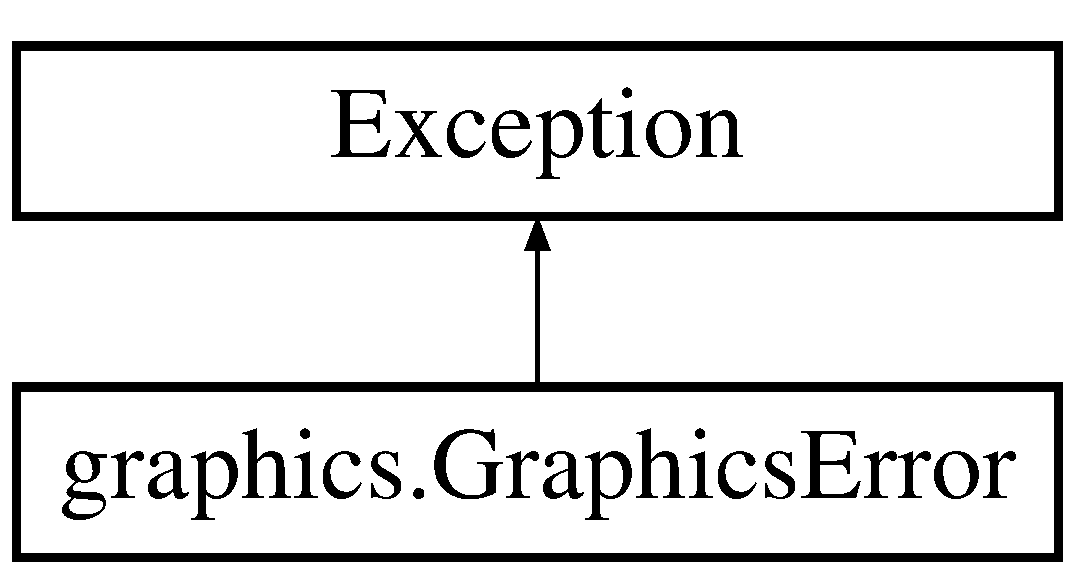
\includegraphics[height=2.000000cm]{classgraphics_1_1_graphics_error}
\end{center}
\end{figure}


\subsection{Detailed Description}
Module Exceptions. 

\begin{DoxyVerb}Generic error class for graphics module exceptions.\end{DoxyVerb}
 

The documentation for this class was generated from the following file\+:\begin{DoxyCompactItemize}
\item 
graphics.\+py\end{DoxyCompactItemize}

\hypertarget{classgraphics_1_1_graphics_object}{}\section{graphics.\+Graphics\+Object Class Reference}
\label{classgraphics_1_1_graphics_object}\index{graphics.\+Graphics\+Object@{graphics.\+Graphics\+Object}}
Inheritance diagram for graphics.\+Graphics\+Object\+:\begin{figure}[H]
\begin{center}
\leavevmode
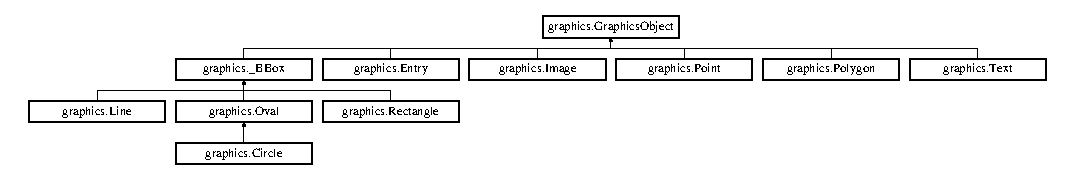
\includegraphics[height=1.987578cm]{classgraphics_1_1_graphics_object}
\end{center}
\end{figure}
\subsection*{Public Member Functions}
\begin{DoxyCompactItemize}
\item 
def {\bfseries \+\_\+\+\_\+init\+\_\+\+\_\+} (self, options)\hypertarget{classgraphics_1_1_graphics_object_a87c93d91bf82269f0b31c1e669b7ddf4}{}\label{classgraphics_1_1_graphics_object_a87c93d91bf82269f0b31c1e669b7ddf4}

\item 
def \hyperlink{classgraphics_1_1_graphics_object_acfba33cbf63f5333f961b86e988fc292}{set\+Fill} (self, color)
\item 
def \hyperlink{classgraphics_1_1_graphics_object_a0acf1399e539cc273170096552a04139}{set\+Outline} (self, color)
\item 
def \hyperlink{classgraphics_1_1_graphics_object_a63006871dd6242bfc7aabe9ddcbb1263}{set\+Width} (self, width)
\item 
def \hyperlink{classgraphics_1_1_graphics_object_ac7849154dccab74cb76d2a28035db48c}{draw} (self, graphwin)
\item 
def \hyperlink{classgraphics_1_1_graphics_object_a7dc6432aa782c84f61407362e579aaf5}{undraw} (self)
\item 
def \hyperlink{classgraphics_1_1_graphics_object_a2dc26fc41e5fa51c7a97b592da2926e8}{move} (self, dx, dy)
\end{DoxyCompactItemize}
\subsection*{Public Attributes}
\begin{DoxyCompactItemize}
\item 
{\bfseries canvas}\hypertarget{classgraphics_1_1_graphics_object_a961312a5609642e6d96b892e9b5755e3}{}\label{classgraphics_1_1_graphics_object_a961312a5609642e6d96b892e9b5755e3}

\item 
{\bfseries id}\hypertarget{classgraphics_1_1_graphics_object_a465597cb2472214302bfa13c7708e217}{}\label{classgraphics_1_1_graphics_object_a465597cb2472214302bfa13c7708e217}

\item 
{\bfseries config}\hypertarget{classgraphics_1_1_graphics_object_a329ba44d4b0347a6f62eb4559110540a}{}\label{classgraphics_1_1_graphics_object_a329ba44d4b0347a6f62eb4559110540a}

\end{DoxyCompactItemize}


\subsection{Detailed Description}
\begin{DoxyVerb}Generic base class for all of the drawable objects\end{DoxyVerb}
 

\subsection{Member Function Documentation}
\index{graphics\+::\+Graphics\+Object@{graphics\+::\+Graphics\+Object}!draw@{draw}}
\index{draw@{draw}!graphics\+::\+Graphics\+Object@{graphics\+::\+Graphics\+Object}}
\subsubsection[{\texorpdfstring{draw(self, graphwin)}{draw(self, graphwin)}}]{\setlength{\rightskip}{0pt plus 5cm}def graphics.\+Graphics\+Object.\+draw (
\begin{DoxyParamCaption}
\item[{}]{self, }
\item[{}]{graphwin}
\end{DoxyParamCaption}
)}\hypertarget{classgraphics_1_1_graphics_object_ac7849154dccab74cb76d2a28035db48c}{}\label{classgraphics_1_1_graphics_object_ac7849154dccab74cb76d2a28035db48c}
\begin{DoxyVerb}Draw the object in graphwin, which should be a GraphWin
object.  A GraphicsObject may only be drawn into one
window. Raises an error if attempt made to draw an object that
is already visible.\end{DoxyVerb}
 \index{graphics\+::\+Graphics\+Object@{graphics\+::\+Graphics\+Object}!move@{move}}
\index{move@{move}!graphics\+::\+Graphics\+Object@{graphics\+::\+Graphics\+Object}}
\subsubsection[{\texorpdfstring{move(self, dx, dy)}{move(self, dx, dy)}}]{\setlength{\rightskip}{0pt plus 5cm}def graphics.\+Graphics\+Object.\+move (
\begin{DoxyParamCaption}
\item[{}]{self, }
\item[{}]{dx, }
\item[{}]{dy}
\end{DoxyParamCaption}
)}\hypertarget{classgraphics_1_1_graphics_object_a2dc26fc41e5fa51c7a97b592da2926e8}{}\label{classgraphics_1_1_graphics_object_a2dc26fc41e5fa51c7a97b592da2926e8}
\begin{DoxyVerb}move object dx units in x direction and dy units in y
direction\end{DoxyVerb}
 \index{graphics\+::\+Graphics\+Object@{graphics\+::\+Graphics\+Object}!set\+Fill@{set\+Fill}}
\index{set\+Fill@{set\+Fill}!graphics\+::\+Graphics\+Object@{graphics\+::\+Graphics\+Object}}
\subsubsection[{\texorpdfstring{set\+Fill(self, color)}{setFill(self, color)}}]{\setlength{\rightskip}{0pt plus 5cm}def graphics.\+Graphics\+Object.\+set\+Fill (
\begin{DoxyParamCaption}
\item[{}]{self, }
\item[{}]{color}
\end{DoxyParamCaption}
)}\hypertarget{classgraphics_1_1_graphics_object_acfba33cbf63f5333f961b86e988fc292}{}\label{classgraphics_1_1_graphics_object_acfba33cbf63f5333f961b86e988fc292}
\begin{DoxyVerb}Set interior color to color\end{DoxyVerb}
 \index{graphics\+::\+Graphics\+Object@{graphics\+::\+Graphics\+Object}!set\+Outline@{set\+Outline}}
\index{set\+Outline@{set\+Outline}!graphics\+::\+Graphics\+Object@{graphics\+::\+Graphics\+Object}}
\subsubsection[{\texorpdfstring{set\+Outline(self, color)}{setOutline(self, color)}}]{\setlength{\rightskip}{0pt plus 5cm}def graphics.\+Graphics\+Object.\+set\+Outline (
\begin{DoxyParamCaption}
\item[{}]{self, }
\item[{}]{color}
\end{DoxyParamCaption}
)}\hypertarget{classgraphics_1_1_graphics_object_a0acf1399e539cc273170096552a04139}{}\label{classgraphics_1_1_graphics_object_a0acf1399e539cc273170096552a04139}
\begin{DoxyVerb}Set outline color to color\end{DoxyVerb}
 \index{graphics\+::\+Graphics\+Object@{graphics\+::\+Graphics\+Object}!set\+Width@{set\+Width}}
\index{set\+Width@{set\+Width}!graphics\+::\+Graphics\+Object@{graphics\+::\+Graphics\+Object}}
\subsubsection[{\texorpdfstring{set\+Width(self, width)}{setWidth(self, width)}}]{\setlength{\rightskip}{0pt plus 5cm}def graphics.\+Graphics\+Object.\+set\+Width (
\begin{DoxyParamCaption}
\item[{}]{self, }
\item[{}]{width}
\end{DoxyParamCaption}
)}\hypertarget{classgraphics_1_1_graphics_object_a63006871dd6242bfc7aabe9ddcbb1263}{}\label{classgraphics_1_1_graphics_object_a63006871dd6242bfc7aabe9ddcbb1263}
\begin{DoxyVerb}Set line weight to width\end{DoxyVerb}
 \index{graphics\+::\+Graphics\+Object@{graphics\+::\+Graphics\+Object}!undraw@{undraw}}
\index{undraw@{undraw}!graphics\+::\+Graphics\+Object@{graphics\+::\+Graphics\+Object}}
\subsubsection[{\texorpdfstring{undraw(self)}{undraw(self)}}]{\setlength{\rightskip}{0pt plus 5cm}def graphics.\+Graphics\+Object.\+undraw (
\begin{DoxyParamCaption}
\item[{}]{self}
\end{DoxyParamCaption}
)}\hypertarget{classgraphics_1_1_graphics_object_a7dc6432aa782c84f61407362e579aaf5}{}\label{classgraphics_1_1_graphics_object_a7dc6432aa782c84f61407362e579aaf5}
\begin{DoxyVerb}Undraw the object (i.e. hide it). Returns silently if the
object is not currently drawn.\end{DoxyVerb}
 

The documentation for this class was generated from the following file\+:\begin{DoxyCompactItemize}
\item 
graphics.\+py\end{DoxyCompactItemize}

\hypertarget{classgraphics_1_1_graph_win}{}\section{graphics.\+Graph\+Win Class Reference}
\label{classgraphics_1_1_graph_win}\index{graphics.\+Graph\+Win@{graphics.\+Graph\+Win}}


Graphics classes start here.  


Inheritance diagram for graphics.\+Graph\+Win\+:\begin{figure}[H]
\begin{center}
\leavevmode
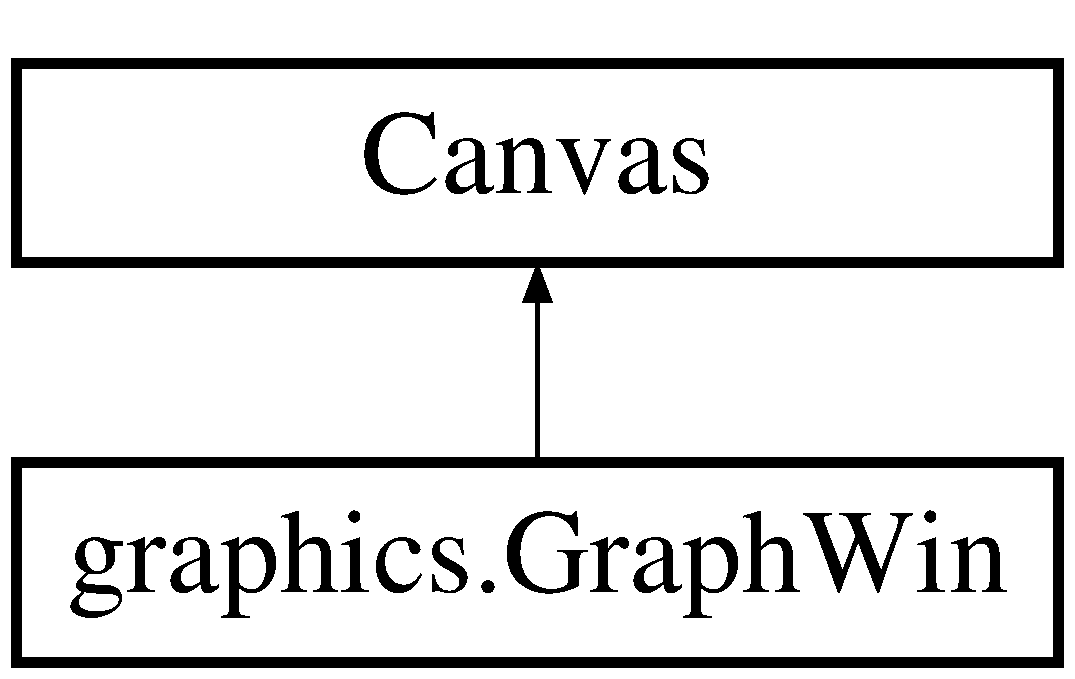
\includegraphics[height=2.000000cm]{classgraphics_1_1_graph_win}
\end{center}
\end{figure}
\subsection*{Public Member Functions}
\begin{DoxyCompactItemize}
\item 
def {\bfseries \+\_\+\+\_\+init\+\_\+\+\_\+} (self, title=\char`\"{}Graphics Window\char`\"{}, width=200, height=200, autoflush=True)\hypertarget{classgraphics_1_1_graph_win_abaf17e0a7d09fe97cbb23f03ca545339}{}\label{classgraphics_1_1_graph_win_abaf17e0a7d09fe97cbb23f03ca545339}

\item 
def {\bfseries \+\_\+\+\_\+repr\+\_\+\+\_\+} (self)\hypertarget{classgraphics_1_1_graph_win_afc6d29fa1772c46ec5f1c8917c0dfa36}{}\label{classgraphics_1_1_graph_win_afc6d29fa1772c46ec5f1c8917c0dfa36}

\item 
def {\bfseries \+\_\+\+\_\+str\+\_\+\+\_\+} (self)\hypertarget{classgraphics_1_1_graph_win_a47a25afdbc0a778241b364142caf862e}{}\label{classgraphics_1_1_graph_win_a47a25afdbc0a778241b364142caf862e}

\item 
def \hyperlink{classgraphics_1_1_graph_win_aec4e7921def91d795367eef63054a4df}{set\+Background} (self, color)
\item 
def \hyperlink{classgraphics_1_1_graph_win_a9f5ef08db39c026392b093c2d0a7fbe9}{set\+Coords} (self, x1, y1, x2, y2)
\item 
def \hyperlink{classgraphics_1_1_graph_win_a760daa823490308117c5ce3ea2946bfb}{close} (self)
\item 
def {\bfseries is\+Closed} (self)\hypertarget{classgraphics_1_1_graph_win_a77f97f64e8d3dddcef5d3c345ffedc6d}{}\label{classgraphics_1_1_graph_win_a77f97f64e8d3dddcef5d3c345ffedc6d}

\item 
def {\bfseries is\+Open} (self)\hypertarget{classgraphics_1_1_graph_win_a1a3732b58c2ffc8960be3a9f66bd4df8}{}\label{classgraphics_1_1_graph_win_a1a3732b58c2ffc8960be3a9f66bd4df8}

\item 
def \hyperlink{classgraphics_1_1_graph_win_ac93adafee6ea1c0d9bb32b64cfbe754c}{plot} (self, x, y, color=\char`\"{}black\char`\"{})
\item 
def \hyperlink{classgraphics_1_1_graph_win_a66ef7f9b272d4ef482f834855ccfa0c4}{plot\+Pixel} (self, x, y, color=\char`\"{}black\char`\"{})
\item 
def \hyperlink{classgraphics_1_1_graph_win_a232137e7f2464c4ed6fa4a6fd5022196}{flush} (self)
\item 
def \hyperlink{classgraphics_1_1_graph_win_a4fdf1cf728e9aa559f2912592f66c23e}{get\+Mouse} (self)
\item 
def \hyperlink{classgraphics_1_1_graph_win_a47a21f43176302d35e418810c88235ea}{check\+Mouse} (self)
\item 
def \hyperlink{classgraphics_1_1_graph_win_adf821f120ef3baf805a4945b009b4903}{get\+Key} (self)
\item 
def \hyperlink{classgraphics_1_1_graph_win_a84c703d3a1521fc5edb4fd8af462ebd1}{check\+Key} (self)
\item 
def \hyperlink{classgraphics_1_1_graph_win_a100d08973109234fa8b17ccc0ac3ff89}{get\+Height} (self)
\item 
def \hyperlink{classgraphics_1_1_graph_win_a5bad6bf8b35250baf4f4b45993f85162}{get\+Width} (self)
\item 
def {\bfseries to\+Screen} (self, x, y)\hypertarget{classgraphics_1_1_graph_win_a4dfd70dc27ff32544c0eee0e73f52c36}{}\label{classgraphics_1_1_graph_win_a4dfd70dc27ff32544c0eee0e73f52c36}

\item 
def {\bfseries to\+World} (self, x, y)\hypertarget{classgraphics_1_1_graph_win_a6c40e111bf739598f2128c95977caff7}{}\label{classgraphics_1_1_graph_win_a6c40e111bf739598f2128c95977caff7}

\item 
def {\bfseries set\+Mouse\+Handler} (self, func)\hypertarget{classgraphics_1_1_graph_win_a6b0162764403abcbb64d3de5a8e21c1c}{}\label{classgraphics_1_1_graph_win_a6b0162764403abcbb64d3de5a8e21c1c}

\item 
def {\bfseries add\+Item} (self, item)\hypertarget{classgraphics_1_1_graph_win_acb38179ff82c99fe11e5150e2fbbf1e4}{}\label{classgraphics_1_1_graph_win_acb38179ff82c99fe11e5150e2fbbf1e4}

\item 
def {\bfseries del\+Item} (self, item)\hypertarget{classgraphics_1_1_graph_win_a617ee0e44a58c66c06df5d4d51edbee5}{}\label{classgraphics_1_1_graph_win_a617ee0e44a58c66c06df5d4d51edbee5}

\item 
def {\bfseries redraw} (self)\hypertarget{classgraphics_1_1_graph_win_afd181d963aa18c8f8215c114d6124b72}{}\label{classgraphics_1_1_graph_win_afd181d963aa18c8f8215c114d6124b72}

\end{DoxyCompactItemize}
\subsection*{Public Attributes}
\begin{DoxyCompactItemize}
\item 
{\bfseries foreground}\hypertarget{classgraphics_1_1_graph_win_acd60a861291a9a2a0357422052de423e}{}\label{classgraphics_1_1_graph_win_acd60a861291a9a2a0357422052de423e}

\item 
{\bfseries items}\hypertarget{classgraphics_1_1_graph_win_aa5eb438d0f6bcf9b48cf752bc970492d}{}\label{classgraphics_1_1_graph_win_aa5eb438d0f6bcf9b48cf752bc970492d}

\item 
{\bfseries mouseX}\hypertarget{classgraphics_1_1_graph_win_a048ee90a088e92ea85449aa4e2dc14e8}{}\label{classgraphics_1_1_graph_win_a048ee90a088e92ea85449aa4e2dc14e8}

\item 
{\bfseries mouseY}\hypertarget{classgraphics_1_1_graph_win_a6c44740c795384fad61d1d5a3465d4f5}{}\label{classgraphics_1_1_graph_win_a6c44740c795384fad61d1d5a3465d4f5}

\item 
{\bfseries height}\hypertarget{classgraphics_1_1_graph_win_ac54dcaf8cf4b5d8d4e50ba66636e3804}{}\label{classgraphics_1_1_graph_win_ac54dcaf8cf4b5d8d4e50ba66636e3804}

\item 
{\bfseries width}\hypertarget{classgraphics_1_1_graph_win_a8725576095977a7867e61028bf67168a}{}\label{classgraphics_1_1_graph_win_a8725576095977a7867e61028bf67168a}

\item 
{\bfseries autoflush}\hypertarget{classgraphics_1_1_graph_win_a678b9a9c46f93e11dc5f76c8503c7888}{}\label{classgraphics_1_1_graph_win_a678b9a9c46f93e11dc5f76c8503c7888}

\item 
{\bfseries trans}\hypertarget{classgraphics_1_1_graph_win_abceec8568a7d09be0d0461bd32a15225}{}\label{classgraphics_1_1_graph_win_abceec8568a7d09be0d0461bd32a15225}

\item 
{\bfseries closed}\hypertarget{classgraphics_1_1_graph_win_aa479363c78ec2ffd05065887abd5851e}{}\label{classgraphics_1_1_graph_win_aa479363c78ec2ffd05065887abd5851e}

\item 
{\bfseries last\+Key}\hypertarget{classgraphics_1_1_graph_win_a345868afb0c992bd31b20b02e6593bbb}{}\label{classgraphics_1_1_graph_win_a345868afb0c992bd31b20b02e6593bbb}

\end{DoxyCompactItemize}


\subsection{Detailed Description}
Graphics classes start here. 

\begin{DoxyVerb}A GraphWin is a toplevel window for displaying graphics.\end{DoxyVerb}
 

\subsection{Member Function Documentation}
\index{graphics\+::\+Graph\+Win@{graphics\+::\+Graph\+Win}!check\+Key@{check\+Key}}
\index{check\+Key@{check\+Key}!graphics\+::\+Graph\+Win@{graphics\+::\+Graph\+Win}}
\subsubsection[{\texorpdfstring{check\+Key(self)}{checkKey(self)}}]{\setlength{\rightskip}{0pt plus 5cm}def graphics.\+Graph\+Win.\+check\+Key (
\begin{DoxyParamCaption}
\item[{}]{self}
\end{DoxyParamCaption}
)}\hypertarget{classgraphics_1_1_graph_win_a84c703d3a1521fc5edb4fd8af462ebd1}{}\label{classgraphics_1_1_graph_win_a84c703d3a1521fc5edb4fd8af462ebd1}
\begin{DoxyVerb}Return last key pressed or None if no key pressed since last call\end{DoxyVerb}
 \index{graphics\+::\+Graph\+Win@{graphics\+::\+Graph\+Win}!check\+Mouse@{check\+Mouse}}
\index{check\+Mouse@{check\+Mouse}!graphics\+::\+Graph\+Win@{graphics\+::\+Graph\+Win}}
\subsubsection[{\texorpdfstring{check\+Mouse(self)}{checkMouse(self)}}]{\setlength{\rightskip}{0pt plus 5cm}def graphics.\+Graph\+Win.\+check\+Mouse (
\begin{DoxyParamCaption}
\item[{}]{self}
\end{DoxyParamCaption}
)}\hypertarget{classgraphics_1_1_graph_win_a47a21f43176302d35e418810c88235ea}{}\label{classgraphics_1_1_graph_win_a47a21f43176302d35e418810c88235ea}
\begin{DoxyVerb}Return last mouse click or None if mouse has
not been clicked since last call\end{DoxyVerb}
 \index{graphics\+::\+Graph\+Win@{graphics\+::\+Graph\+Win}!close@{close}}
\index{close@{close}!graphics\+::\+Graph\+Win@{graphics\+::\+Graph\+Win}}
\subsubsection[{\texorpdfstring{close(self)}{close(self)}}]{\setlength{\rightskip}{0pt plus 5cm}def graphics.\+Graph\+Win.\+close (
\begin{DoxyParamCaption}
\item[{}]{self}
\end{DoxyParamCaption}
)}\hypertarget{classgraphics_1_1_graph_win_a760daa823490308117c5ce3ea2946bfb}{}\label{classgraphics_1_1_graph_win_a760daa823490308117c5ce3ea2946bfb}
\begin{DoxyVerb}Close the window\end{DoxyVerb}
 \index{graphics\+::\+Graph\+Win@{graphics\+::\+Graph\+Win}!flush@{flush}}
\index{flush@{flush}!graphics\+::\+Graph\+Win@{graphics\+::\+Graph\+Win}}
\subsubsection[{\texorpdfstring{flush(self)}{flush(self)}}]{\setlength{\rightskip}{0pt plus 5cm}def graphics.\+Graph\+Win.\+flush (
\begin{DoxyParamCaption}
\item[{}]{self}
\end{DoxyParamCaption}
)}\hypertarget{classgraphics_1_1_graph_win_a232137e7f2464c4ed6fa4a6fd5022196}{}\label{classgraphics_1_1_graph_win_a232137e7f2464c4ed6fa4a6fd5022196}
\begin{DoxyVerb}Update drawing to the window\end{DoxyVerb}
 \index{graphics\+::\+Graph\+Win@{graphics\+::\+Graph\+Win}!get\+Height@{get\+Height}}
\index{get\+Height@{get\+Height}!graphics\+::\+Graph\+Win@{graphics\+::\+Graph\+Win}}
\subsubsection[{\texorpdfstring{get\+Height(self)}{getHeight(self)}}]{\setlength{\rightskip}{0pt plus 5cm}def graphics.\+Graph\+Win.\+get\+Height (
\begin{DoxyParamCaption}
\item[{}]{self}
\end{DoxyParamCaption}
)}\hypertarget{classgraphics_1_1_graph_win_a100d08973109234fa8b17ccc0ac3ff89}{}\label{classgraphics_1_1_graph_win_a100d08973109234fa8b17ccc0ac3ff89}
\begin{DoxyVerb}Return the height of the window\end{DoxyVerb}
 \index{graphics\+::\+Graph\+Win@{graphics\+::\+Graph\+Win}!get\+Key@{get\+Key}}
\index{get\+Key@{get\+Key}!graphics\+::\+Graph\+Win@{graphics\+::\+Graph\+Win}}
\subsubsection[{\texorpdfstring{get\+Key(self)}{getKey(self)}}]{\setlength{\rightskip}{0pt plus 5cm}def graphics.\+Graph\+Win.\+get\+Key (
\begin{DoxyParamCaption}
\item[{}]{self}
\end{DoxyParamCaption}
)}\hypertarget{classgraphics_1_1_graph_win_adf821f120ef3baf805a4945b009b4903}{}\label{classgraphics_1_1_graph_win_adf821f120ef3baf805a4945b009b4903}
\begin{DoxyVerb}Wait for user to press a key and return it as a string.\end{DoxyVerb}
 \index{graphics\+::\+Graph\+Win@{graphics\+::\+Graph\+Win}!get\+Mouse@{get\+Mouse}}
\index{get\+Mouse@{get\+Mouse}!graphics\+::\+Graph\+Win@{graphics\+::\+Graph\+Win}}
\subsubsection[{\texorpdfstring{get\+Mouse(self)}{getMouse(self)}}]{\setlength{\rightskip}{0pt plus 5cm}def graphics.\+Graph\+Win.\+get\+Mouse (
\begin{DoxyParamCaption}
\item[{}]{self}
\end{DoxyParamCaption}
)}\hypertarget{classgraphics_1_1_graph_win_a4fdf1cf728e9aa559f2912592f66c23e}{}\label{classgraphics_1_1_graph_win_a4fdf1cf728e9aa559f2912592f66c23e}
\begin{DoxyVerb}Wait for mouse click and return Point object representing
the click\end{DoxyVerb}
 \index{graphics\+::\+Graph\+Win@{graphics\+::\+Graph\+Win}!get\+Width@{get\+Width}}
\index{get\+Width@{get\+Width}!graphics\+::\+Graph\+Win@{graphics\+::\+Graph\+Win}}
\subsubsection[{\texorpdfstring{get\+Width(self)}{getWidth(self)}}]{\setlength{\rightskip}{0pt plus 5cm}def graphics.\+Graph\+Win.\+get\+Width (
\begin{DoxyParamCaption}
\item[{}]{self}
\end{DoxyParamCaption}
)}\hypertarget{classgraphics_1_1_graph_win_a5bad6bf8b35250baf4f4b45993f85162}{}\label{classgraphics_1_1_graph_win_a5bad6bf8b35250baf4f4b45993f85162}
\begin{DoxyVerb}Return the width of the window\end{DoxyVerb}
 \index{graphics\+::\+Graph\+Win@{graphics\+::\+Graph\+Win}!plot@{plot}}
\index{plot@{plot}!graphics\+::\+Graph\+Win@{graphics\+::\+Graph\+Win}}
\subsubsection[{\texorpdfstring{plot(self, x, y, color=""black"")}{plot(self, x, y, color="black")}}]{\setlength{\rightskip}{0pt plus 5cm}def graphics.\+Graph\+Win.\+plot (
\begin{DoxyParamCaption}
\item[{}]{self, }
\item[{}]{x, }
\item[{}]{y, }
\item[{}]{color = {\ttfamily \char`\"{}black\char`\"{}}}
\end{DoxyParamCaption}
)}\hypertarget{classgraphics_1_1_graph_win_ac93adafee6ea1c0d9bb32b64cfbe754c}{}\label{classgraphics_1_1_graph_win_ac93adafee6ea1c0d9bb32b64cfbe754c}
\begin{DoxyVerb}Set pixel (x,y) to the given color\end{DoxyVerb}
 \index{graphics\+::\+Graph\+Win@{graphics\+::\+Graph\+Win}!plot\+Pixel@{plot\+Pixel}}
\index{plot\+Pixel@{plot\+Pixel}!graphics\+::\+Graph\+Win@{graphics\+::\+Graph\+Win}}
\subsubsection[{\texorpdfstring{plot\+Pixel(self, x, y, color=""black"")}{plotPixel(self, x, y, color="black")}}]{\setlength{\rightskip}{0pt plus 5cm}def graphics.\+Graph\+Win.\+plot\+Pixel (
\begin{DoxyParamCaption}
\item[{}]{self, }
\item[{}]{x, }
\item[{}]{y, }
\item[{}]{color = {\ttfamily \char`\"{}black\char`\"{}}}
\end{DoxyParamCaption}
)}\hypertarget{classgraphics_1_1_graph_win_a66ef7f9b272d4ef482f834855ccfa0c4}{}\label{classgraphics_1_1_graph_win_a66ef7f9b272d4ef482f834855ccfa0c4}
\begin{DoxyVerb}Set pixel raw (independent of window coordinates) pixel
(x,y) to color\end{DoxyVerb}
 \index{graphics\+::\+Graph\+Win@{graphics\+::\+Graph\+Win}!set\+Background@{set\+Background}}
\index{set\+Background@{set\+Background}!graphics\+::\+Graph\+Win@{graphics\+::\+Graph\+Win}}
\subsubsection[{\texorpdfstring{set\+Background(self, color)}{setBackground(self, color)}}]{\setlength{\rightskip}{0pt plus 5cm}def graphics.\+Graph\+Win.\+set\+Background (
\begin{DoxyParamCaption}
\item[{}]{self, }
\item[{}]{color}
\end{DoxyParamCaption}
)}\hypertarget{classgraphics_1_1_graph_win_aec4e7921def91d795367eef63054a4df}{}\label{classgraphics_1_1_graph_win_aec4e7921def91d795367eef63054a4df}
\begin{DoxyVerb}Set background color of the window\end{DoxyVerb}
 \index{graphics\+::\+Graph\+Win@{graphics\+::\+Graph\+Win}!set\+Coords@{set\+Coords}}
\index{set\+Coords@{set\+Coords}!graphics\+::\+Graph\+Win@{graphics\+::\+Graph\+Win}}
\subsubsection[{\texorpdfstring{set\+Coords(self, x1, y1, x2, y2)}{setCoords(self, x1, y1, x2, y2)}}]{\setlength{\rightskip}{0pt plus 5cm}def graphics.\+Graph\+Win.\+set\+Coords (
\begin{DoxyParamCaption}
\item[{}]{self, }
\item[{}]{x1, }
\item[{}]{y1, }
\item[{}]{x2, }
\item[{}]{y2}
\end{DoxyParamCaption}
)}\hypertarget{classgraphics_1_1_graph_win_a9f5ef08db39c026392b093c2d0a7fbe9}{}\label{classgraphics_1_1_graph_win_a9f5ef08db39c026392b093c2d0a7fbe9}
\begin{DoxyVerb}Set coordinates of window to run from (x1,y1) in the
lower-left corner to (x2,y2) in the upper-right corner.\end{DoxyVerb}
 

The documentation for this class was generated from the following file\+:\begin{DoxyCompactItemize}
\item 
graphics.\+py\end{DoxyCompactItemize}

\hypertarget{class_parsing_classes_actual_1_1_if_statement}{}\section{Parsing\+Classes\+Actual.\+If\+Statement Class Reference}
\label{class_parsing_classes_actual_1_1_if_statement}\index{Parsing\+Classes\+Actual.\+If\+Statement@{Parsing\+Classes\+Actual.\+If\+Statement}}


class representing control flow which executes first statement whose condition is found true  


\subsection*{Public Member Functions}
\begin{DoxyCompactItemize}
\item 
def \hyperlink{class_parsing_classes_actual_1_1_if_statement_adcb418725eec33d6e81784b67c1fe776}{\+\_\+\+\_\+init\+\_\+\+\_\+} (self, listof\+Conditionals)
\begin{DoxyCompactList}\small\item\em the constructor \end{DoxyCompactList}\item 
def \hyperlink{class_parsing_classes_actual_1_1_if_statement_aede84cbec163184d403eb3626c08ed41}{exec} (self)\hypertarget{class_parsing_classes_actual_1_1_if_statement_aede84cbec163184d403eb3626c08ed41}{}\label{class_parsing_classes_actual_1_1_if_statement_aede84cbec163184d403eb3626c08ed41}

\begin{DoxyCompactList}\small\item\em The executable which runs until it finds the first true condtion, following which that block is executed. \end{DoxyCompactList}\end{DoxyCompactItemize}
\subsection*{Public Attributes}
\begin{DoxyCompactItemize}
\item 
{\bfseries listof\+Conditionals}\hypertarget{class_parsing_classes_actual_1_1_if_statement_a4b1d2d5524d305d12c7bee2d03f7877d}{}\label{class_parsing_classes_actual_1_1_if_statement_a4b1d2d5524d305d12c7bee2d03f7877d}

\end{DoxyCompactItemize}


\subsection{Detailed Description}
class representing control flow which executes first statement whose condition is found true 

\subsection{Constructor \& Destructor Documentation}
\index{Parsing\+Classes\+Actual\+::\+If\+Statement@{Parsing\+Classes\+Actual\+::\+If\+Statement}!\+\_\+\+\_\+init\+\_\+\+\_\+@{\+\_\+\+\_\+init\+\_\+\+\_\+}}
\index{\+\_\+\+\_\+init\+\_\+\+\_\+@{\+\_\+\+\_\+init\+\_\+\+\_\+}!Parsing\+Classes\+Actual\+::\+If\+Statement@{Parsing\+Classes\+Actual\+::\+If\+Statement}}
\subsubsection[{\texorpdfstring{\+\_\+\+\_\+init\+\_\+\+\_\+(self, listof\+Conditionals)}{__init__(self, listofConditionals)}}]{\setlength{\rightskip}{0pt plus 5cm}def Parsing\+Classes\+Actual.\+If\+Statement.\+\_\+\+\_\+init\+\_\+\+\_\+ (
\begin{DoxyParamCaption}
\item[{}]{self, }
\item[{}]{listof\+Conditionals}
\end{DoxyParamCaption}
)}\hypertarget{class_parsing_classes_actual_1_1_if_statement_adcb418725eec33d6e81784b67c1fe776}{}\label{class_parsing_classes_actual_1_1_if_statement_adcb418725eec33d6e81784b67c1fe776}


the constructor 


\begin{DoxyParams}{Parameters}
{\em listof\+Conditionals} & List of tuples containing the condition and the statemnet\+List to be implemented if it is true \\
\hline
\end{DoxyParams}


The documentation for this class was generated from the following file\+:\begin{DoxyCompactItemize}
\item 
Parsing\+Classes\+Actual.\+py\end{DoxyCompactItemize}

\hypertarget{classparser_classes_1_1_if_statement}{}\section{parser\+Classes.\+If\+Statement Class Reference}
\label{classparser_classes_1_1_if_statement}\index{parser\+Classes.\+If\+Statement@{parser\+Classes.\+If\+Statement}}
\subsection*{Public Member Functions}
\begin{DoxyCompactItemize}
\item 
def {\bfseries \+\_\+\+\_\+init\+\_\+\+\_\+} (self, listof\+Conditionals)\hypertarget{classparser_classes_1_1_if_statement_a53d538b0688ee1556bcda14383ff7a1c}{}\label{classparser_classes_1_1_if_statement_a53d538b0688ee1556bcda14383ff7a1c}

\item 
def {\bfseries exec} (self)\hypertarget{classparser_classes_1_1_if_statement_a53a8b4b35816147f44d1d1e568f60528}{}\label{classparser_classes_1_1_if_statement_a53a8b4b35816147f44d1d1e568f60528}

\end{DoxyCompactItemize}
\subsection*{Public Attributes}
\begin{DoxyCompactItemize}
\item 
{\bfseries listof\+Conditionals}\hypertarget{classparser_classes_1_1_if_statement_a9d440106c71d7c46441ad74cf7142a25}{}\label{classparser_classes_1_1_if_statement_a9d440106c71d7c46441ad74cf7142a25}

\end{DoxyCompactItemize}


The documentation for this class was generated from the following file\+:\begin{DoxyCompactItemize}
\item 
parser\+Classes.\+py\end{DoxyCompactItemize}

\hypertarget{classgraphics_1_1_image}{}\section{graphics.\+Image Class Reference}
\label{classgraphics_1_1_image}\index{graphics.\+Image@{graphics.\+Image}}
Inheritance diagram for graphics.\+Image\+:\begin{figure}[H]
\begin{center}
\leavevmode
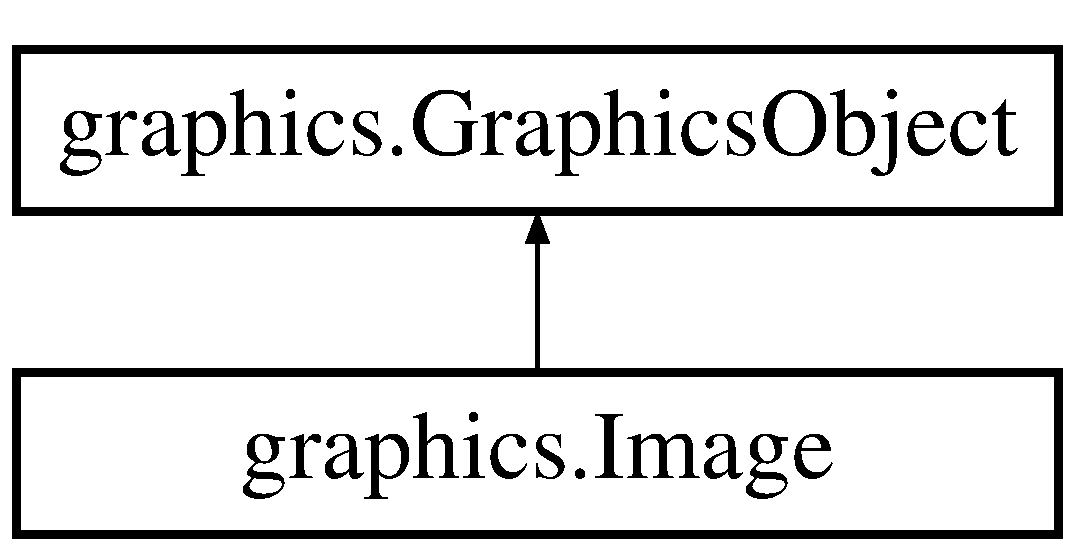
\includegraphics[height=2.000000cm]{classgraphics_1_1_image}
\end{center}
\end{figure}
\subsection*{Public Member Functions}
\begin{DoxyCompactItemize}
\item 
def {\bfseries \+\_\+\+\_\+init\+\_\+\+\_\+} (self, p, pixmap)\hypertarget{classgraphics_1_1_image_a0e82c34ead99ecc7e8bd19f8d073c135}{}\label{classgraphics_1_1_image_a0e82c34ead99ecc7e8bd19f8d073c135}

\item 
def {\bfseries \+\_\+\+\_\+repr\+\_\+\+\_\+} (self)\hypertarget{classgraphics_1_1_image_a6dc7689939ebef91fbce7ff60b190a32}{}\label{classgraphics_1_1_image_a6dc7689939ebef91fbce7ff60b190a32}

\item 
def {\bfseries undraw} (self)\hypertarget{classgraphics_1_1_image_a012595b97cd10d26b7fa2f0f0460d169}{}\label{classgraphics_1_1_image_a012595b97cd10d26b7fa2f0f0460d169}

\item 
def {\bfseries get\+Anchor} (self)\hypertarget{classgraphics_1_1_image_a7f5afb0cad91db822c5074255eb53f04}{}\label{classgraphics_1_1_image_a7f5afb0cad91db822c5074255eb53f04}

\item 
def {\bfseries clone} (self)\hypertarget{classgraphics_1_1_image_a4ade7cc782c157e45fa9b516fe6a3a98}{}\label{classgraphics_1_1_image_a4ade7cc782c157e45fa9b516fe6a3a98}

\item 
def \hyperlink{classgraphics_1_1_image_aff8e62ceeb4265e4d17ce852903c9ae3}{get\+Width} (self)
\item 
def \hyperlink{classgraphics_1_1_image_ab092ccc35755f176309971023f912d67}{get\+Height} (self)
\item 
def \hyperlink{classgraphics_1_1_image_a69deca3f65e378be239eb1ba837d06f8}{get\+Pixel} (self, x, y)
\item 
def \hyperlink{classgraphics_1_1_image_a73fb3ce4de03fe9f57c076d739712378}{set\+Pixel} (self, x, y, color)
\item 
def \hyperlink{classgraphics_1_1_image_ace518e9286a3bc0f81c7f1029c394104}{save} (self, filename)
\end{DoxyCompactItemize}
\subsection*{Public Attributes}
\begin{DoxyCompactItemize}
\item 
{\bfseries anchor}\hypertarget{classgraphics_1_1_image_acc3e91e765b3f90bcfa825cf39b931cd}{}\label{classgraphics_1_1_image_acc3e91e765b3f90bcfa825cf39b931cd}

\item 
{\bfseries image\+Id}\hypertarget{classgraphics_1_1_image_a828ed2128760fd4b813ea80c49bdadb7}{}\label{classgraphics_1_1_image_a828ed2128760fd4b813ea80c49bdadb7}

\item 
{\bfseries img}\hypertarget{classgraphics_1_1_image_a9accbb024d2332c73737270a6c50e402}{}\label{classgraphics_1_1_image_a9accbb024d2332c73737270a6c50e402}

\end{DoxyCompactItemize}
\subsection*{Static Public Attributes}
\begin{DoxyCompactItemize}
\item 
int {\bfseries id\+Count} = 0\hypertarget{classgraphics_1_1_image_a258028ba5c61bd2f207b60479b8e88a6}{}\label{classgraphics_1_1_image_a258028ba5c61bd2f207b60479b8e88a6}

\item 
dictionary {\bfseries image\+Cache} = \{\}\hypertarget{classgraphics_1_1_image_a7a552e05624726d285476348222c32d4}{}\label{classgraphics_1_1_image_a7a552e05624726d285476348222c32d4}

\end{DoxyCompactItemize}


\subsection{Member Function Documentation}
\index{graphics\+::\+Image@{graphics\+::\+Image}!get\+Height@{get\+Height}}
\index{get\+Height@{get\+Height}!graphics\+::\+Image@{graphics\+::\+Image}}
\subsubsection[{\texorpdfstring{get\+Height(self)}{getHeight(self)}}]{\setlength{\rightskip}{0pt plus 5cm}def graphics.\+Image.\+get\+Height (
\begin{DoxyParamCaption}
\item[{}]{self}
\end{DoxyParamCaption}
)}\hypertarget{classgraphics_1_1_image_ab092ccc35755f176309971023f912d67}{}\label{classgraphics_1_1_image_ab092ccc35755f176309971023f912d67}
\begin{DoxyVerb}Returns the height of the image in pixels\end{DoxyVerb}
 \index{graphics\+::\+Image@{graphics\+::\+Image}!get\+Pixel@{get\+Pixel}}
\index{get\+Pixel@{get\+Pixel}!graphics\+::\+Image@{graphics\+::\+Image}}
\subsubsection[{\texorpdfstring{get\+Pixel(self, x, y)}{getPixel(self, x, y)}}]{\setlength{\rightskip}{0pt plus 5cm}def graphics.\+Image.\+get\+Pixel (
\begin{DoxyParamCaption}
\item[{}]{self, }
\item[{}]{x, }
\item[{}]{y}
\end{DoxyParamCaption}
)}\hypertarget{classgraphics_1_1_image_a69deca3f65e378be239eb1ba837d06f8}{}\label{classgraphics_1_1_image_a69deca3f65e378be239eb1ba837d06f8}
\begin{DoxyVerb}Returns a list [r,g,b] with the RGB color values for pixel (x,y)
r,g,b are in range(256)\end{DoxyVerb}
 \index{graphics\+::\+Image@{graphics\+::\+Image}!get\+Width@{get\+Width}}
\index{get\+Width@{get\+Width}!graphics\+::\+Image@{graphics\+::\+Image}}
\subsubsection[{\texorpdfstring{get\+Width(self)}{getWidth(self)}}]{\setlength{\rightskip}{0pt plus 5cm}def graphics.\+Image.\+get\+Width (
\begin{DoxyParamCaption}
\item[{}]{self}
\end{DoxyParamCaption}
)}\hypertarget{classgraphics_1_1_image_aff8e62ceeb4265e4d17ce852903c9ae3}{}\label{classgraphics_1_1_image_aff8e62ceeb4265e4d17ce852903c9ae3}
\begin{DoxyVerb}Returns the width of the image in pixels\end{DoxyVerb}
 \index{graphics\+::\+Image@{graphics\+::\+Image}!save@{save}}
\index{save@{save}!graphics\+::\+Image@{graphics\+::\+Image}}
\subsubsection[{\texorpdfstring{save(self, filename)}{save(self, filename)}}]{\setlength{\rightskip}{0pt plus 5cm}def graphics.\+Image.\+save (
\begin{DoxyParamCaption}
\item[{}]{self, }
\item[{}]{filename}
\end{DoxyParamCaption}
)}\hypertarget{classgraphics_1_1_image_ace518e9286a3bc0f81c7f1029c394104}{}\label{classgraphics_1_1_image_ace518e9286a3bc0f81c7f1029c394104}
\begin{DoxyVerb}Saves the pixmap image to filename.
The format for the save image is determined from the filname extension.\end{DoxyVerb}
 \index{graphics\+::\+Image@{graphics\+::\+Image}!set\+Pixel@{set\+Pixel}}
\index{set\+Pixel@{set\+Pixel}!graphics\+::\+Image@{graphics\+::\+Image}}
\subsubsection[{\texorpdfstring{set\+Pixel(self, x, y, color)}{setPixel(self, x, y, color)}}]{\setlength{\rightskip}{0pt plus 5cm}def graphics.\+Image.\+set\+Pixel (
\begin{DoxyParamCaption}
\item[{}]{self, }
\item[{}]{x, }
\item[{}]{y, }
\item[{}]{color}
\end{DoxyParamCaption}
)}\hypertarget{classgraphics_1_1_image_a73fb3ce4de03fe9f57c076d739712378}{}\label{classgraphics_1_1_image_a73fb3ce4de03fe9f57c076d739712378}
\begin{DoxyVerb}Sets pixel (x,y) to the given color\end{DoxyVerb}
 

The documentation for this class was generated from the following file\+:\begin{DoxyCompactItemize}
\item 
graphics.\+py\end{DoxyCompactItemize}

\hypertarget{class_parsing_classes_actual_1_1_int}{}\section{Parsing\+Classes\+Actual.\+Int Class Reference}
\label{class_parsing_classes_actual_1_1_int}\index{Parsing\+Classes\+Actual.\+Int@{Parsing\+Classes\+Actual.\+Int}}


class for int datatype  


Inheritance diagram for Parsing\+Classes\+Actual.\+Int\+:\begin{figure}[H]
\begin{center}
\leavevmode
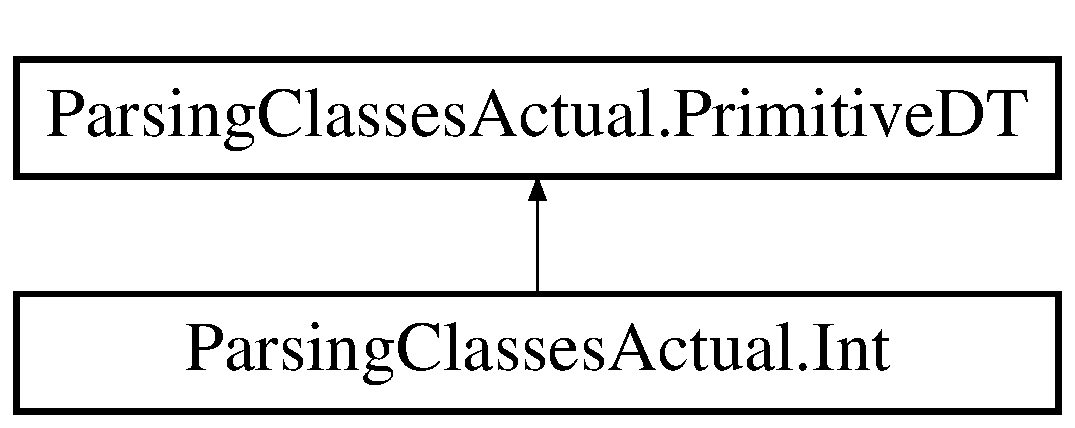
\includegraphics[height=2.000000cm]{class_parsing_classes_actual_1_1_int}
\end{center}
\end{figure}
\subsection*{Public Member Functions}
\begin{DoxyCompactItemize}
\item 
def \hyperlink{class_parsing_classes_actual_1_1_int_a138d3ed5b3b5bcc5f3aeeef5716a1c42}{\+\_\+\+\_\+init\+\_\+\+\_\+} (self, value=0)
\begin{DoxyCompactList}\small\item\em the constructor \end{DoxyCompactList}\item 
\mbox{\Hypertarget{class_parsing_classes_actual_1_1_int_a6430fbdf4a89ea8c64b08c5d69c3ac1a}\label{class_parsing_classes_actual_1_1_int_a6430fbdf4a89ea8c64b08c5d69c3ac1a}} 
def \hyperlink{class_parsing_classes_actual_1_1_int_a6430fbdf4a89ea8c64b08c5d69c3ac1a}{give\+Type} (self)
\begin{DoxyCompactList}\small\item\em returns the type of value \end{DoxyCompactList}\item 
\mbox{\Hypertarget{class_parsing_classes_actual_1_1_int_a9dd15ae2f1ef3e3452d307013b439744}\label{class_parsing_classes_actual_1_1_int_a9dd15ae2f1ef3e3452d307013b439744}} 
def \hyperlink{class_parsing_classes_actual_1_1_int_a9dd15ae2f1ef3e3452d307013b439744}{update} (self, val)
\begin{DoxyCompactList}\small\item\em updates the stored value by typecasting it \end{DoxyCompactList}\end{DoxyCompactItemize}
\subsection*{Public Attributes}
\begin{DoxyCompactItemize}
\item 
\mbox{\Hypertarget{class_parsing_classes_actual_1_1_int_a87fd8a55e3d9dfc9799793ddb57fe340}\label{class_parsing_classes_actual_1_1_int_a87fd8a55e3d9dfc9799793ddb57fe340}} 
{\bfseries value}
\end{DoxyCompactItemize}


\subsection{Detailed Description}
class for int datatype 

\subsection{Constructor \& Destructor Documentation}
\mbox{\Hypertarget{class_parsing_classes_actual_1_1_int_a138d3ed5b3b5bcc5f3aeeef5716a1c42}\label{class_parsing_classes_actual_1_1_int_a138d3ed5b3b5bcc5f3aeeef5716a1c42}} 
\index{Parsing\+Classes\+Actual\+::\+Int@{Parsing\+Classes\+Actual\+::\+Int}!\+\_\+\+\_\+init\+\_\+\+\_\+@{\+\_\+\+\_\+init\+\_\+\+\_\+}}
\index{\+\_\+\+\_\+init\+\_\+\+\_\+@{\+\_\+\+\_\+init\+\_\+\+\_\+}!Parsing\+Classes\+Actual\+::\+Int@{Parsing\+Classes\+Actual\+::\+Int}}
\subsubsection{\texorpdfstring{\+\_\+\+\_\+init\+\_\+\+\_\+()}{\_\_init\_\_()}}
{\footnotesize\ttfamily def Parsing\+Classes\+Actual.\+Int.\+\_\+\+\_\+init\+\_\+\+\_\+ (\begin{DoxyParamCaption}\item[{}]{self,  }\item[{}]{value = {\ttfamily 0} }\end{DoxyParamCaption})}



the constructor 


\begin{DoxyParams}{Parameters}
{\em the} & value of datatype \\
\hline
\end{DoxyParams}


The documentation for this class was generated from the following file\+:\begin{DoxyCompactItemize}
\item 
Parsing\+Classes\+Actual.\+py\end{DoxyCompactItemize}

\hypertarget{classparser_classes_1_1_int}{}\section{parser\+Classes.\+Int Class Reference}
\label{classparser_classes_1_1_int}\index{parser\+Classes.\+Int@{parser\+Classes.\+Int}}
Inheritance diagram for parser\+Classes.\+Int\+:\begin{figure}[H]
\begin{center}
\leavevmode
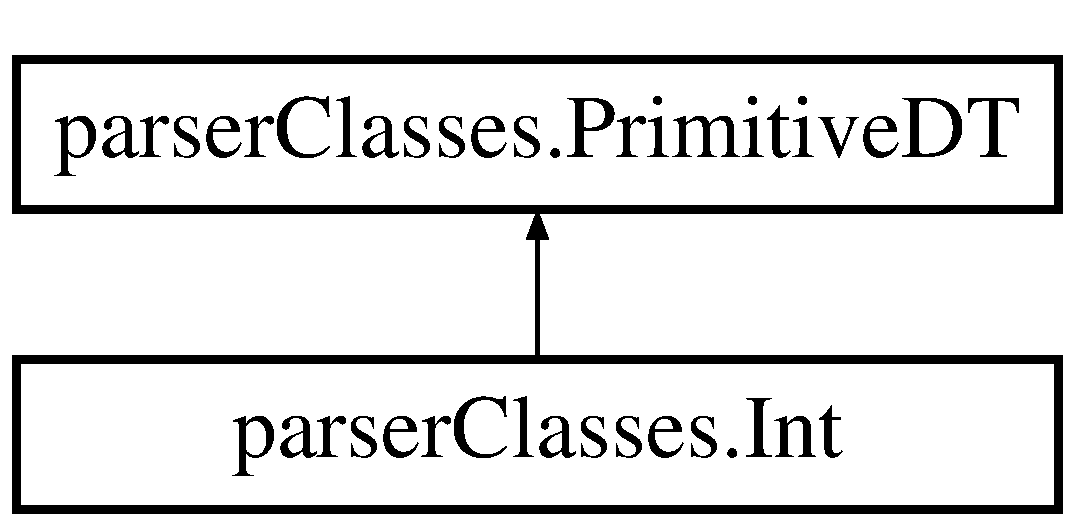
\includegraphics[height=2.000000cm]{classparser_classes_1_1_int}
\end{center}
\end{figure}
\subsection*{Public Member Functions}
\begin{DoxyCompactItemize}
\item 
def {\bfseries \+\_\+\+\_\+init\+\_\+\+\_\+} (self, value=0)\hypertarget{classparser_classes_1_1_int_a5f3c93887c93af55258fd75d55f79120}{}\label{classparser_classes_1_1_int_a5f3c93887c93af55258fd75d55f79120}

\item 
def {\bfseries give\+Type} (self)\hypertarget{classparser_classes_1_1_int_afb7baec715a32b42a3365226fd95e8d1}{}\label{classparser_classes_1_1_int_afb7baec715a32b42a3365226fd95e8d1}

\item 
def {\bfseries update} (self, val)\hypertarget{classparser_classes_1_1_int_a0d695c67593f926a8336ba1b3222f9c8}{}\label{classparser_classes_1_1_int_a0d695c67593f926a8336ba1b3222f9c8}

\end{DoxyCompactItemize}
\subsection*{Public Attributes}
\begin{DoxyCompactItemize}
\item 
{\bfseries value}\hypertarget{classparser_classes_1_1_int_a3daf0c4b136a333cb9f496272fffd119}{}\label{classparser_classes_1_1_int_a3daf0c4b136a333cb9f496272fffd119}

\end{DoxyCompactItemize}


The documentation for this class was generated from the following file\+:\begin{DoxyCompactItemize}
\item 
parser\+Classes.\+py\end{DoxyCompactItemize}

\hypertarget{classgraphics_1_1_line}{}\section{graphics.\+Line Class Reference}
\label{classgraphics_1_1_line}\index{graphics.\+Line@{graphics.\+Line}}
Inheritance diagram for graphics.\+Line\+:\begin{figure}[H]
\begin{center}
\leavevmode
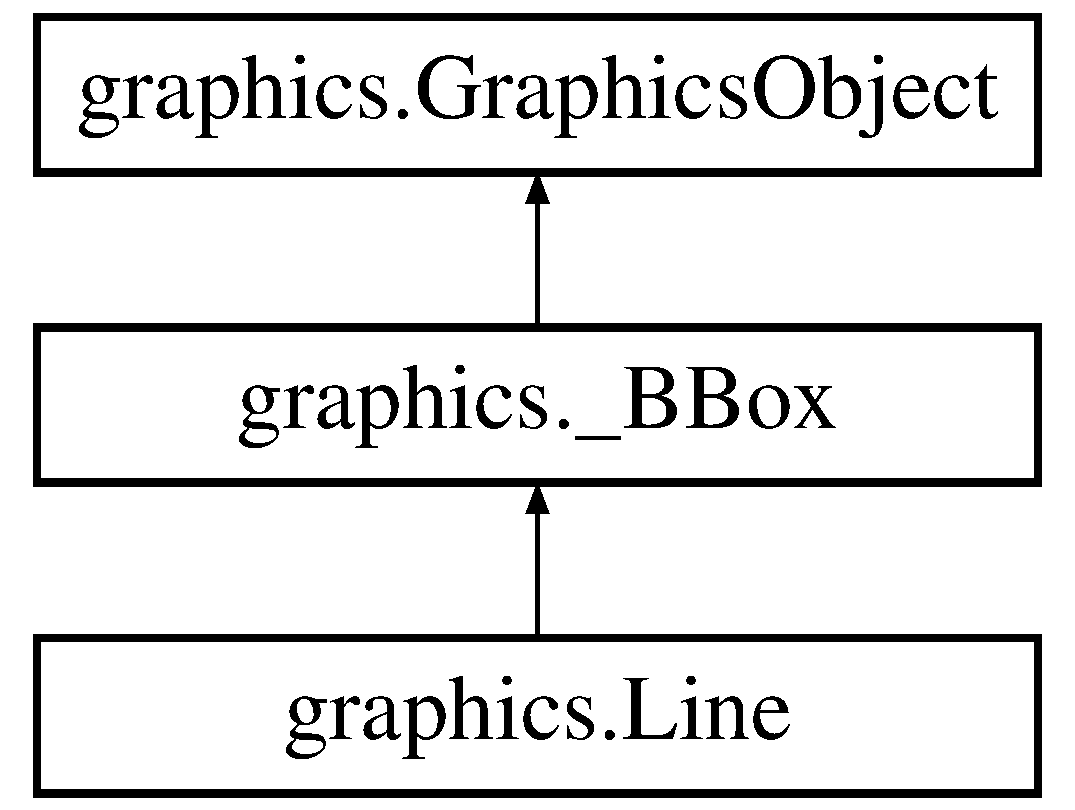
\includegraphics[height=3.000000cm]{classgraphics_1_1_line}
\end{center}
\end{figure}
\subsection*{Public Member Functions}
\begin{DoxyCompactItemize}
\item 
\mbox{\Hypertarget{classgraphics_1_1_line_a8aab9ed90de9a987a2ea6446caca2188}\label{classgraphics_1_1_line_a8aab9ed90de9a987a2ea6446caca2188}} 
def {\bfseries \+\_\+\+\_\+init\+\_\+\+\_\+} (self, p1, p2)
\item 
\mbox{\Hypertarget{classgraphics_1_1_line_a9f0196b56e225e7c1688b55486848ad5}\label{classgraphics_1_1_line_a9f0196b56e225e7c1688b55486848ad5}} 
def {\bfseries \+\_\+\+\_\+repr\+\_\+\+\_\+} (self)
\item 
\mbox{\Hypertarget{classgraphics_1_1_line_a2691c6ba64cfb04f32a585d40f1a7e1e}\label{classgraphics_1_1_line_a2691c6ba64cfb04f32a585d40f1a7e1e}} 
def {\bfseries clone} (self)
\item 
\mbox{\Hypertarget{classgraphics_1_1_line_aef621dc2bfe50449ac764fda18ede3b6}\label{classgraphics_1_1_line_aef621dc2bfe50449ac764fda18ede3b6}} 
def {\bfseries set\+Arrow} (self, option)
\end{DoxyCompactItemize}
\subsection*{Public Attributes}
\begin{DoxyCompactItemize}
\item 
\mbox{\Hypertarget{classgraphics_1_1_line_a2462ca216d643515e7956d8e3688bf44}\label{classgraphics_1_1_line_a2462ca216d643515e7956d8e3688bf44}} 
{\bfseries set\+Outline}
\end{DoxyCompactItemize}


The documentation for this class was generated from the following file\+:\begin{DoxyCompactItemize}
\item 
graphics.\+py\end{DoxyCompactItemize}

\hypertarget{class_parsing_classes_actual_1_1_member__function}{}\section{Parsing\+Classes\+Actual.\+Member\+\_\+function Class Reference}
\label{class_parsing_classes_actual_1_1_member__function}\index{Parsing\+Classes\+Actual.\+Member\+\_\+function@{Parsing\+Classes\+Actual.\+Member\+\_\+function}}
\subsection*{Public Member Functions}
\begin{DoxyCompactItemize}
\item 
def {\bfseries \+\_\+\+\_\+init\+\_\+\+\_\+} (self, req\+Data, snippet)\hypertarget{class_parsing_classes_actual_1_1_member__function_abebf3cf5db29a8776c3144d7a7cf4fac}{}\label{class_parsing_classes_actual_1_1_member__function_abebf3cf5db29a8776c3144d7a7cf4fac}

\item 
def {\bfseries eval} (self)\hypertarget{class_parsing_classes_actual_1_1_member__function_a33449b8ca04728cd8fe854830aa1d730}{}\label{class_parsing_classes_actual_1_1_member__function_a33449b8ca04728cd8fe854830aa1d730}

\item 
def {\bfseries exec} (self)\hypertarget{class_parsing_classes_actual_1_1_member__function_aafcfb847d09b4dc16428bf10dd596bc1}{}\label{class_parsing_classes_actual_1_1_member__function_aafcfb847d09b4dc16428bf10dd596bc1}

\end{DoxyCompactItemize}
\subsection*{Public Attributes}
\begin{DoxyCompactItemize}
\item 
{\bfseries name}\hypertarget{class_parsing_classes_actual_1_1_member__function_ab05a5b7f454a630168fa27b9b543200d}{}\label{class_parsing_classes_actual_1_1_member__function_ab05a5b7f454a630168fa27b9b543200d}

\item 
{\bfseries functname}\hypertarget{class_parsing_classes_actual_1_1_member__function_a92b7dd050cca1f1fc59553b4f3d45223}{}\label{class_parsing_classes_actual_1_1_member__function_a92b7dd050cca1f1fc59553b4f3d45223}

\item 
{\bfseries snippet}\hypertarget{class_parsing_classes_actual_1_1_member__function_a819f607e7531d89e9c5954567e8373f8}{}\label{class_parsing_classes_actual_1_1_member__function_a819f607e7531d89e9c5954567e8373f8}

\end{DoxyCompactItemize}


The documentation for this class was generated from the following file\+:\begin{DoxyCompactItemize}
\item 
Parsing\+Classes\+Actual.\+py\end{DoxyCompactItemize}

\hypertarget{classparser_classes_1_1_member__function}{}\section{parser\+Classes.\+Member\+\_\+function Class Reference}
\label{classparser_classes_1_1_member__function}\index{parser\+Classes.\+Member\+\_\+function@{parser\+Classes.\+Member\+\_\+function}}
\subsection*{Public Member Functions}
\begin{DoxyCompactItemize}
\item 
\mbox{\Hypertarget{classparser_classes_1_1_member__function_a497b32d0e46480abd8f4f573ee68a3b0}\label{classparser_classes_1_1_member__function_a497b32d0e46480abd8f4f573ee68a3b0}} 
def {\bfseries \+\_\+\+\_\+init\+\_\+\+\_\+} (self, req\+Data)
\item 
\mbox{\Hypertarget{classparser_classes_1_1_member__function_ae132533c55122b32a25746696db39249}\label{classparser_classes_1_1_member__function_ae132533c55122b32a25746696db39249}} 
def {\bfseries eval} (self)
\item 
\mbox{\Hypertarget{classparser_classes_1_1_member__function_aa938612d9582fb3851370a7680f84efe}\label{classparser_classes_1_1_member__function_aa938612d9582fb3851370a7680f84efe}} 
def {\bfseries exec} (self)
\end{DoxyCompactItemize}
\subsection*{Public Attributes}
\begin{DoxyCompactItemize}
\item 
\mbox{\Hypertarget{classparser_classes_1_1_member__function_a3937d00f545419b14a3807f66fb89a8b}\label{classparser_classes_1_1_member__function_a3937d00f545419b14a3807f66fb89a8b}} 
{\bfseries name}
\item 
\mbox{\Hypertarget{classparser_classes_1_1_member__function_a01cc4459bfeab553a8fb2c3f99110b7e}\label{classparser_classes_1_1_member__function_a01cc4459bfeab553a8fb2c3f99110b7e}} 
{\bfseries functname}
\end{DoxyCompactItemize}


The documentation for this class was generated from the following file\+:\begin{DoxyCompactItemize}
\item 
parser\+Classes.\+py\end{DoxyCompactItemize}

\hypertarget{class_parsing_classes_actual_1_1_multiple__member__function}{}\section{Parsing\+Classes\+Actual.\+Multiple\+\_\+member\+\_\+function Class Reference}
\label{class_parsing_classes_actual_1_1_multiple__member__function}\index{Parsing\+Classes\+Actual.\+Multiple\+\_\+member\+\_\+function@{Parsing\+Classes\+Actual.\+Multiple\+\_\+member\+\_\+function}}
\subsection*{Public Member Functions}
\begin{DoxyCompactItemize}
\item 
\mbox{\Hypertarget{class_parsing_classes_actual_1_1_multiple__member__function_a27da0e19523b0219e7d58cd7dbabc9a9}\label{class_parsing_classes_actual_1_1_multiple__member__function_a27da0e19523b0219e7d58cd7dbabc9a9}} 
def {\bfseries \+\_\+\+\_\+init\+\_\+\+\_\+} (self, req\+Data, snippet)
\item 
\mbox{\Hypertarget{class_parsing_classes_actual_1_1_multiple__member__function_a8d3e7a3f25b30947e82604271ad6c49d}\label{class_parsing_classes_actual_1_1_multiple__member__function_a8d3e7a3f25b30947e82604271ad6c49d}} 
def {\bfseries eval} (self)
\item 
\mbox{\Hypertarget{class_parsing_classes_actual_1_1_multiple__member__function_a3bc26d567ef38186228536c4234281ec}\label{class_parsing_classes_actual_1_1_multiple__member__function_a3bc26d567ef38186228536c4234281ec}} 
def {\bfseries exec} (self)
\end{DoxyCompactItemize}
\subsection*{Public Attributes}
\begin{DoxyCompactItemize}
\item 
\mbox{\Hypertarget{class_parsing_classes_actual_1_1_multiple__member__function_a8d1095e288eba5cd271dd0300590ecc5}\label{class_parsing_classes_actual_1_1_multiple__member__function_a8d1095e288eba5cd271dd0300590ecc5}} 
{\bfseries name}
\item 
\mbox{\Hypertarget{class_parsing_classes_actual_1_1_multiple__member__function_afe344b4cf0e1d608d4e5697364bcbd93}\label{class_parsing_classes_actual_1_1_multiple__member__function_afe344b4cf0e1d608d4e5697364bcbd93}} 
{\bfseries functname}
\item 
\mbox{\Hypertarget{class_parsing_classes_actual_1_1_multiple__member__function_a19dfea13ddeb0c4340b987575e5f2402}\label{class_parsing_classes_actual_1_1_multiple__member__function_a19dfea13ddeb0c4340b987575e5f2402}} 
{\bfseries arguements}
\item 
\mbox{\Hypertarget{class_parsing_classes_actual_1_1_multiple__member__function_a766af60b5f794ead87ffcc726b50466e}\label{class_parsing_classes_actual_1_1_multiple__member__function_a766af60b5f794ead87ffcc726b50466e}} 
{\bfseries snippet}
\end{DoxyCompactItemize}


The documentation for this class was generated from the following file\+:\begin{DoxyCompactItemize}
\item 
Parsing\+Classes\+Actual.\+py\end{DoxyCompactItemize}

\hypertarget{classparser_classes_1_1_multiple__member__function}{}\section{parser\+Classes.\+Multiple\+\_\+member\+\_\+function Class Reference}
\label{classparser_classes_1_1_multiple__member__function}\index{parser\+Classes.\+Multiple\+\_\+member\+\_\+function@{parser\+Classes.\+Multiple\+\_\+member\+\_\+function}}
\subsection*{Public Member Functions}
\begin{DoxyCompactItemize}
\item 
def {\bfseries \+\_\+\+\_\+init\+\_\+\+\_\+} (self, req\+Data)\hypertarget{classparser_classes_1_1_multiple__member__function_a49138664c1c079a08daebd21d676616f}{}\label{classparser_classes_1_1_multiple__member__function_a49138664c1c079a08daebd21d676616f}

\item 
def {\bfseries eval} (self)\hypertarget{classparser_classes_1_1_multiple__member__function_abbd74e3f6048c0feabfe52e257cbd91a}{}\label{classparser_classes_1_1_multiple__member__function_abbd74e3f6048c0feabfe52e257cbd91a}

\item 
def {\bfseries exec} (self)\hypertarget{classparser_classes_1_1_multiple__member__function_a158a2a6d96d99c42350fe9245614a9ee}{}\label{classparser_classes_1_1_multiple__member__function_a158a2a6d96d99c42350fe9245614a9ee}

\end{DoxyCompactItemize}
\subsection*{Public Attributes}
\begin{DoxyCompactItemize}
\item 
{\bfseries name}\hypertarget{classparser_classes_1_1_multiple__member__function_a841b86dab291bf9deb8f873f58864f9e}{}\label{classparser_classes_1_1_multiple__member__function_a841b86dab291bf9deb8f873f58864f9e}

\item 
{\bfseries functname}\hypertarget{classparser_classes_1_1_multiple__member__function_a69614fc7d47fe2f241bbe186ac027b56}{}\label{classparser_classes_1_1_multiple__member__function_a69614fc7d47fe2f241bbe186ac027b56}

\item 
{\bfseries arguements}\hypertarget{classparser_classes_1_1_multiple__member__function_a444d7614f6b7aa98ab83c1ff8f1fbe7c}{}\label{classparser_classes_1_1_multiple__member__function_a444d7614f6b7aa98ab83c1ff8f1fbe7c}

\end{DoxyCompactItemize}


The documentation for this class was generated from the following file\+:\begin{DoxyCompactItemize}
\item 
parser\+Classes.\+py\end{DoxyCompactItemize}

\hypertarget{classexecution_stack_1_1_node}{}\section{execution\+Stack.\+Node Class Reference}
\label{classexecution_stack_1_1_node}\index{execution\+Stack.\+Node@{execution\+Stack.\+Node}}
\subsection*{Public Member Functions}
\begin{DoxyCompactItemize}
\item 
def {\bfseries \+\_\+\+\_\+init\+\_\+\+\_\+} (self, x, y, nxt)\hypertarget{classexecution_stack_1_1_node_a06210944064630822c82b75dfbb39b02}{}\label{classexecution_stack_1_1_node_a06210944064630822c82b75dfbb39b02}

\item 
def {\bfseries modify\+Dictionary} (self, dictionary)\hypertarget{classexecution_stack_1_1_node_a8f6113c2ecc9b3750c2623e4f80fbcb6}{}\label{classexecution_stack_1_1_node_a8f6113c2ecc9b3750c2623e4f80fbcb6}

\item 
def {\bfseries add\+Global} (self)\hypertarget{classexecution_stack_1_1_node_ad09bf2598ac130da3d81990e7a3d4033}{}\label{classexecution_stack_1_1_node_ad09bf2598ac130da3d81990e7a3d4033}

\item 
def {\bfseries show\+Dictionary} (self)\hypertarget{classexecution_stack_1_1_node_acce8dc5b25b98507443871806561b712}{}\label{classexecution_stack_1_1_node_acce8dc5b25b98507443871806561b712}

\item 
def {\bfseries add\+Data} (self, key, val)\hypertarget{classexecution_stack_1_1_node_a1edf851a964aeb75e36218af75d84fa5}{}\label{classexecution_stack_1_1_node_a1edf851a964aeb75e36218af75d84fa5}

\item 
def {\bfseries modify\+Data} (self, key, new\+Val)\hypertarget{classexecution_stack_1_1_node_adaa2133dac332801505899ae26425841}{}\label{classexecution_stack_1_1_node_adaa2133dac332801505899ae26425841}

\item 
def {\bfseries delt} (self, key)\hypertarget{classexecution_stack_1_1_node_a4998dd88ab9c688f7d68863d2d7b8f35}{}\label{classexecution_stack_1_1_node_a4998dd88ab9c688f7d68863d2d7b8f35}

\item 
def {\bfseries delete} (self)\hypertarget{classexecution_stack_1_1_node_ade5473ebe64896f68673f0d5830733bb}{}\label{classexecution_stack_1_1_node_ade5473ebe64896f68673f0d5830733bb}

\end{DoxyCompactItemize}
\subsection*{Public Attributes}
\begin{DoxyCompactItemize}
\item 
{\bfseries x}\hypertarget{classexecution_stack_1_1_node_a8ca70df383e047359c263c1a9394da39}{}\label{classexecution_stack_1_1_node_a8ca70df383e047359c263c1a9394da39}

\item 
{\bfseries y}\hypertarget{classexecution_stack_1_1_node_aa03c2980d8176bb3c5517e389365080d}{}\label{classexecution_stack_1_1_node_aa03c2980d8176bb3c5517e389365080d}

\item 
{\bfseries rectangle}\hypertarget{classexecution_stack_1_1_node_a2e607fa5bd3975623dd1f8009866a788}{}\label{classexecution_stack_1_1_node_a2e607fa5bd3975623dd1f8009866a788}

\item 
{\bfseries next}\hypertarget{classexecution_stack_1_1_node_a1e0a6990eb317d06617edb23264c60cf}{}\label{classexecution_stack_1_1_node_a1e0a6990eb317d06617edb23264c60cf}

\item 
{\bfseries data}\hypertarget{classexecution_stack_1_1_node_af39e3478a051e6f4fef2e22cf7e6ed2c}{}\label{classexecution_stack_1_1_node_af39e3478a051e6f4fef2e22cf7e6ed2c}

\end{DoxyCompactItemize}


The documentation for this class was generated from the following file\+:\begin{DoxyCompactItemize}
\item 
execution\+Stack.\+py\end{DoxyCompactItemize}

\hypertarget{classparser_classes_1_1_number}{}\section{parser\+Classes.\+Number Class Reference}
\label{classparser_classes_1_1_number}\index{parser\+Classes.\+Number@{parser\+Classes.\+Number}}
\subsection*{Public Member Functions}
\begin{DoxyCompactItemize}
\item 
def {\bfseries \+\_\+\+\_\+init\+\_\+\+\_\+} (self, value)\hypertarget{classparser_classes_1_1_number_a556755d9d147b3264b9bf21915166ca1}{}\label{classparser_classes_1_1_number_a556755d9d147b3264b9bf21915166ca1}

\item 
def {\bfseries eval} (self)\hypertarget{classparser_classes_1_1_number_ae310cf63d3a1f2e2767189633be8f5ba}{}\label{classparser_classes_1_1_number_ae310cf63d3a1f2e2767189633be8f5ba}

\end{DoxyCompactItemize}
\subsection*{Public Attributes}
\begin{DoxyCompactItemize}
\item 
{\bfseries value}\hypertarget{classparser_classes_1_1_number_ae074c9227b38acb758a77d2f28d644bd}{}\label{classparser_classes_1_1_number_ae074c9227b38acb758a77d2f28d644bd}

\end{DoxyCompactItemize}


The documentation for this class was generated from the following file\+:\begin{DoxyCompactItemize}
\item 
parser\+Classes.\+py\end{DoxyCompactItemize}

\hypertarget{class_parsing_classes_actual_1_1_number}{}\section{Parsing\+Classes\+Actual.\+Number Class Reference}
\label{class_parsing_classes_actual_1_1_number}\index{Parsing\+Classes\+Actual.\+Number@{Parsing\+Classes\+Actual.\+Number}}


The class to store a number.  


\subsection*{Public Member Functions}
\begin{DoxyCompactItemize}
\item 
def \hyperlink{class_parsing_classes_actual_1_1_number_afed3ef381388f6d2db19fec207e2bbf5}{\+\_\+\+\_\+init\+\_\+\+\_\+} (self, value)
\begin{DoxyCompactList}\small\item\em the constructor \end{DoxyCompactList}\item 
def \hyperlink{class_parsing_classes_actual_1_1_number_a77c608400a103e348084417e5a2782ef}{eval} (self)\hypertarget{class_parsing_classes_actual_1_1_number_a77c608400a103e348084417e5a2782ef}{}\label{class_parsing_classes_actual_1_1_number_a77c608400a103e348084417e5a2782ef}

\begin{DoxyCompactList}\small\item\em the eval function that returns the number stored \end{DoxyCompactList}\end{DoxyCompactItemize}
\subsection*{Public Attributes}
\begin{DoxyCompactItemize}
\item 
{\bfseries value}\hypertarget{class_parsing_classes_actual_1_1_number_a88d148e6057e4ed5014e20876a7e8496}{}\label{class_parsing_classes_actual_1_1_number_a88d148e6057e4ed5014e20876a7e8496}

\end{DoxyCompactItemize}


\subsection{Detailed Description}
The class to store a number. 

\subsection{Constructor \& Destructor Documentation}
\index{Parsing\+Classes\+Actual\+::\+Number@{Parsing\+Classes\+Actual\+::\+Number}!\+\_\+\+\_\+init\+\_\+\+\_\+@{\+\_\+\+\_\+init\+\_\+\+\_\+}}
\index{\+\_\+\+\_\+init\+\_\+\+\_\+@{\+\_\+\+\_\+init\+\_\+\+\_\+}!Parsing\+Classes\+Actual\+::\+Number@{Parsing\+Classes\+Actual\+::\+Number}}
\subsubsection[{\texorpdfstring{\+\_\+\+\_\+init\+\_\+\+\_\+(self, value)}{__init__(self, value)}}]{\setlength{\rightskip}{0pt plus 5cm}def Parsing\+Classes\+Actual.\+Number.\+\_\+\+\_\+init\+\_\+\+\_\+ (
\begin{DoxyParamCaption}
\item[{}]{self, }
\item[{}]{value}
\end{DoxyParamCaption}
)}\hypertarget{class_parsing_classes_actual_1_1_number_afed3ef381388f6d2db19fec207e2bbf5}{}\label{class_parsing_classes_actual_1_1_number_afed3ef381388f6d2db19fec207e2bbf5}


the constructor 


\begin{DoxyParams}{Parameters}
{\em self} & the object pointer \\
\hline
{\em value} & The value to be stored in the class \\
\hline
\end{DoxyParams}


The documentation for this class was generated from the following file\+:\begin{DoxyCompactItemize}
\item 
Parsing\+Classes\+Actual.\+py\end{DoxyCompactItemize}

\hypertarget{classgraphics_1_1_oval}{}\section{graphics.\+Oval Class Reference}
\label{classgraphics_1_1_oval}\index{graphics.\+Oval@{graphics.\+Oval}}
Inheritance diagram for graphics.\+Oval\+:\begin{figure}[H]
\begin{center}
\leavevmode
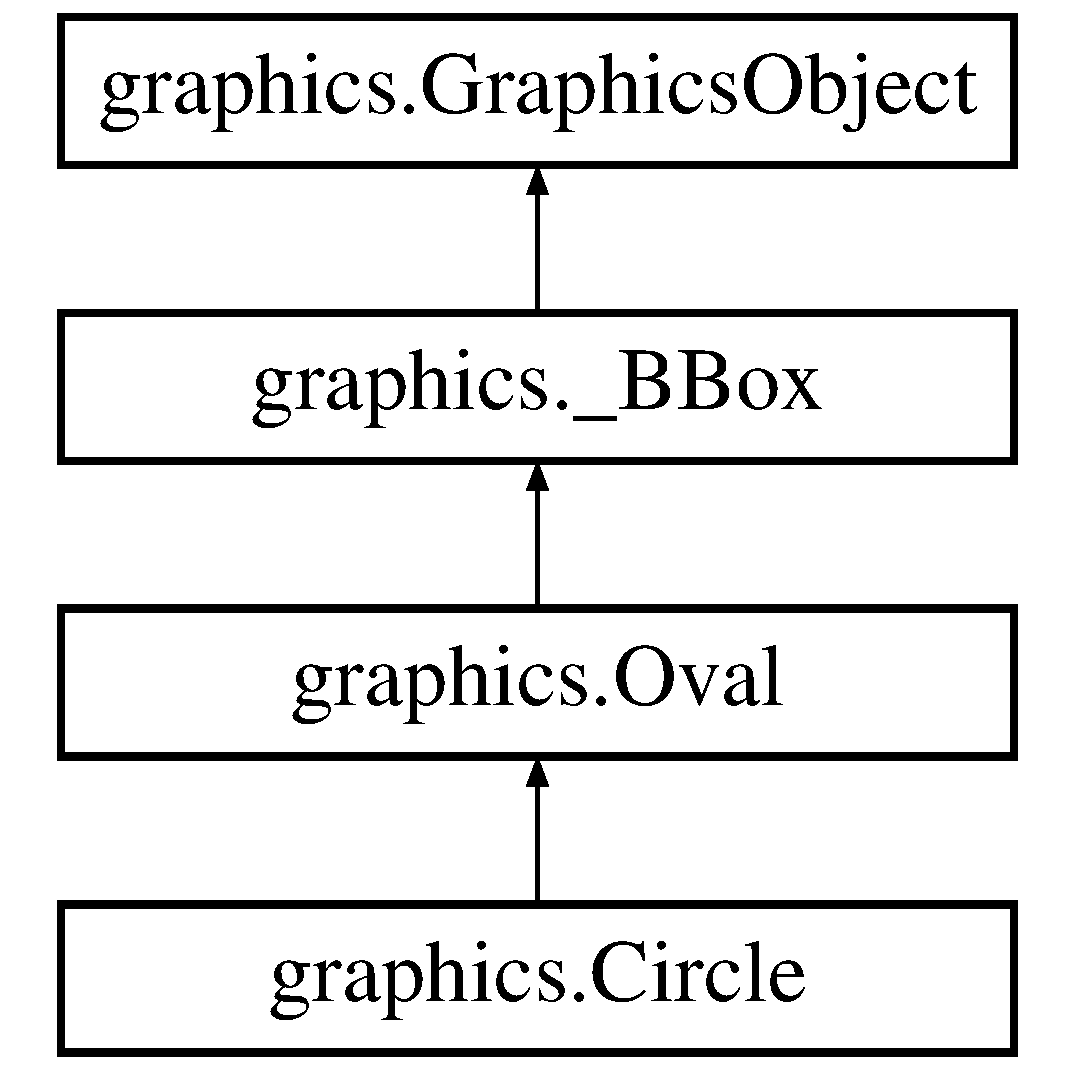
\includegraphics[height=4.000000cm]{classgraphics_1_1_oval}
\end{center}
\end{figure}
\subsection*{Public Member Functions}
\begin{DoxyCompactItemize}
\item 
def {\bfseries \+\_\+\+\_\+init\+\_\+\+\_\+} (self, p1, p2)\hypertarget{classgraphics_1_1_oval_ac24c500a6feba342c3459fbfe5fee794}{}\label{classgraphics_1_1_oval_ac24c500a6feba342c3459fbfe5fee794}

\item 
def {\bfseries \+\_\+\+\_\+repr\+\_\+\+\_\+} (self)\hypertarget{classgraphics_1_1_oval_a7a3e92c1b76ffe75cbc18e49daa159ab}{}\label{classgraphics_1_1_oval_a7a3e92c1b76ffe75cbc18e49daa159ab}

\item 
def {\bfseries clone} (self)\hypertarget{classgraphics_1_1_oval_af914fb35dc36e36f1ba2f43679b8f0a1}{}\label{classgraphics_1_1_oval_af914fb35dc36e36f1ba2f43679b8f0a1}

\end{DoxyCompactItemize}
\subsection*{Additional Inherited Members}


The documentation for this class was generated from the following file\+:\begin{DoxyCompactItemize}
\item 
graphics.\+py\end{DoxyCompactItemize}

\hypertarget{classgraphics_1_1_point}{}\section{graphics.\+Point Class Reference}
\label{classgraphics_1_1_point}\index{graphics.\+Point@{graphics.\+Point}}
Inheritance diagram for graphics.\+Point\+:\begin{figure}[H]
\begin{center}
\leavevmode
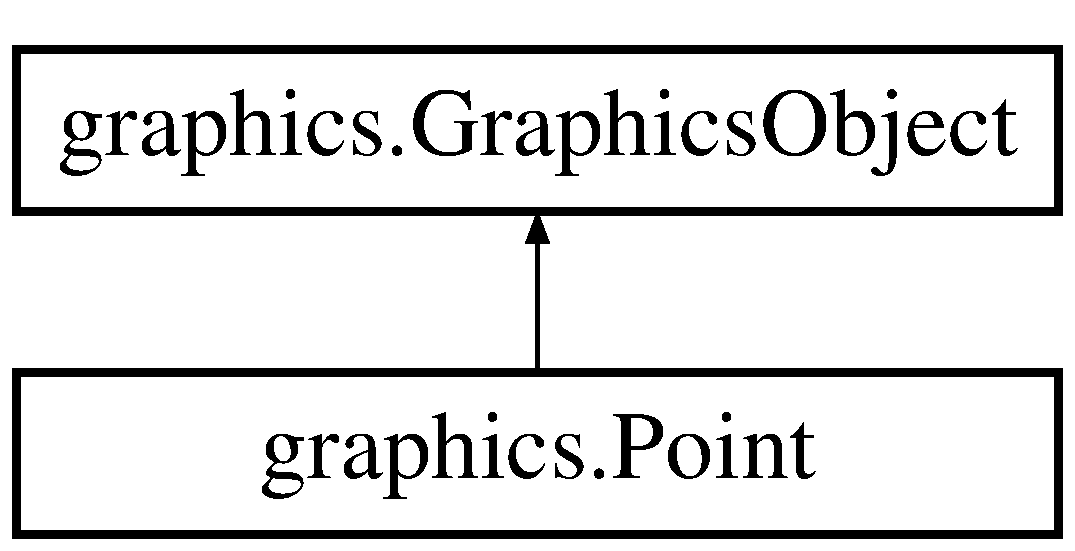
\includegraphics[height=2.000000cm]{classgraphics_1_1_point}
\end{center}
\end{figure}
\subsection*{Public Member Functions}
\begin{DoxyCompactItemize}
\item 
\mbox{\Hypertarget{classgraphics_1_1_point_ab8786043f14e834312522f9a2635ca1c}\label{classgraphics_1_1_point_ab8786043f14e834312522f9a2635ca1c}} 
def {\bfseries \+\_\+\+\_\+init\+\_\+\+\_\+} (self, x, y)
\item 
\mbox{\Hypertarget{classgraphics_1_1_point_a8dabf610e2e2a1ecdcdadfd16d7c42f6}\label{classgraphics_1_1_point_a8dabf610e2e2a1ecdcdadfd16d7c42f6}} 
def {\bfseries \+\_\+\+\_\+repr\+\_\+\+\_\+} (self)
\item 
\mbox{\Hypertarget{classgraphics_1_1_point_a533526af5c8fbfe84c7c0924c4af7fb5}\label{classgraphics_1_1_point_a533526af5c8fbfe84c7c0924c4af7fb5}} 
def {\bfseries clone} (self)
\item 
\mbox{\Hypertarget{classgraphics_1_1_point_a8a19d0055571c7f1d68df9e9624272a6}\label{classgraphics_1_1_point_a8a19d0055571c7f1d68df9e9624272a6}} 
def {\bfseries getX} (self)
\item 
\mbox{\Hypertarget{classgraphics_1_1_point_a48fb2d02f2abf906972cfdae9698fa17}\label{classgraphics_1_1_point_a48fb2d02f2abf906972cfdae9698fa17}} 
def {\bfseries getY} (self)
\end{DoxyCompactItemize}
\subsection*{Public Attributes}
\begin{DoxyCompactItemize}
\item 
\mbox{\Hypertarget{classgraphics_1_1_point_a407fd24b47309128a86e144baa128c09}\label{classgraphics_1_1_point_a407fd24b47309128a86e144baa128c09}} 
{\bfseries set\+Fill}
\item 
\mbox{\Hypertarget{classgraphics_1_1_point_a1ecd4579c57a7a0032a630a96bbe173c}\label{classgraphics_1_1_point_a1ecd4579c57a7a0032a630a96bbe173c}} 
{\bfseries x}
\item 
\mbox{\Hypertarget{classgraphics_1_1_point_a30f1ec4104ee8cb436049ee7aceb8cf4}\label{classgraphics_1_1_point_a30f1ec4104ee8cb436049ee7aceb8cf4}} 
{\bfseries y}
\end{DoxyCompactItemize}


The documentation for this class was generated from the following file\+:\begin{DoxyCompactItemize}
\item 
graphics.\+py\end{DoxyCompactItemize}

\hypertarget{classgraphics_1_1_polygon}{}\section{graphics.\+Polygon Class Reference}
\label{classgraphics_1_1_polygon}\index{graphics.\+Polygon@{graphics.\+Polygon}}
Inheritance diagram for graphics.\+Polygon\+:\begin{figure}[H]
\begin{center}
\leavevmode
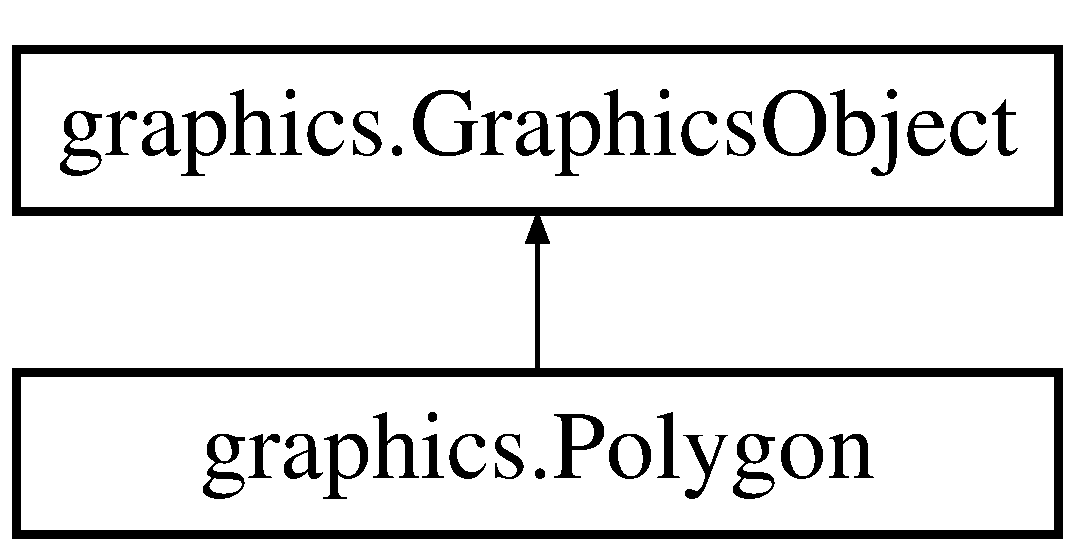
\includegraphics[height=2.000000cm]{classgraphics_1_1_polygon}
\end{center}
\end{figure}
\subsection*{Public Member Functions}
\begin{DoxyCompactItemize}
\item 
def {\bfseries \+\_\+\+\_\+init\+\_\+\+\_\+} (self, points)\hypertarget{classgraphics_1_1_polygon_af9b2f0bcbfecc9d3c2aa5de28c0a3f38}{}\label{classgraphics_1_1_polygon_af9b2f0bcbfecc9d3c2aa5de28c0a3f38}

\item 
def {\bfseries \+\_\+\+\_\+repr\+\_\+\+\_\+} (self)\hypertarget{classgraphics_1_1_polygon_aad12e39fa84c17812be4d1222bf4b33c}{}\label{classgraphics_1_1_polygon_aad12e39fa84c17812be4d1222bf4b33c}

\item 
def {\bfseries clone} (self)\hypertarget{classgraphics_1_1_polygon_aab7a0d81be6f10d4065c9687f5a8b80a}{}\label{classgraphics_1_1_polygon_aab7a0d81be6f10d4065c9687f5a8b80a}

\item 
def {\bfseries get\+Points} (self)\hypertarget{classgraphics_1_1_polygon_a68417042ff193fc01179b274e120d947}{}\label{classgraphics_1_1_polygon_a68417042ff193fc01179b274e120d947}

\end{DoxyCompactItemize}
\subsection*{Public Attributes}
\begin{DoxyCompactItemize}
\item 
{\bfseries points}\hypertarget{classgraphics_1_1_polygon_a3a5ff52b9aef1e15507e2724575da586}{}\label{classgraphics_1_1_polygon_a3a5ff52b9aef1e15507e2724575da586}

\end{DoxyCompactItemize}


The documentation for this class was generated from the following file\+:\begin{DoxyCompactItemize}
\item 
graphics.\+py\end{DoxyCompactItemize}

\hypertarget{classparser_classes_1_1_primitive_declaration}{}\section{parser\+Classes.\+Primitive\+Declaration Class Reference}
\label{classparser_classes_1_1_primitive_declaration}\index{parser\+Classes.\+Primitive\+Declaration@{parser\+Classes.\+Primitive\+Declaration}}
\subsection*{Public Member Functions}
\begin{DoxyCompactItemize}
\item 
def {\bfseries \+\_\+\+\_\+init\+\_\+\+\_\+} (self, var\+Name, var\+Type, var\+Value)\hypertarget{classparser_classes_1_1_primitive_declaration_aad9639eb073bcb44bc75a89c944df91b}{}\label{classparser_classes_1_1_primitive_declaration_aad9639eb073bcb44bc75a89c944df91b}

\item 
def {\bfseries exec} (self)\hypertarget{classparser_classes_1_1_primitive_declaration_a438696675269a0bcb077b6e60acf7bfd}{}\label{classparser_classes_1_1_primitive_declaration_a438696675269a0bcb077b6e60acf7bfd}

\end{DoxyCompactItemize}
\subsection*{Public Attributes}
\begin{DoxyCompactItemize}
\item 
{\bfseries var\+Type}\hypertarget{classparser_classes_1_1_primitive_declaration_af0de807df30562cc04fbd425ea1e2ad1}{}\label{classparser_classes_1_1_primitive_declaration_af0de807df30562cc04fbd425ea1e2ad1}

\item 
{\bfseries var\+Value}\hypertarget{classparser_classes_1_1_primitive_declaration_a2f493d5ebb420d75e5184c520e2fa66b}{}\label{classparser_classes_1_1_primitive_declaration_a2f493d5ebb420d75e5184c520e2fa66b}

\item 
{\bfseries var\+Name}\hypertarget{classparser_classes_1_1_primitive_declaration_abda8fb36580c90aea36e32f8d0785f6c}{}\label{classparser_classes_1_1_primitive_declaration_abda8fb36580c90aea36e32f8d0785f6c}

\end{DoxyCompactItemize}


The documentation for this class was generated from the following file\+:\begin{DoxyCompactItemize}
\item 
parser\+Classes.\+py\end{DoxyCompactItemize}

\hypertarget{class_parsing_classes_actual_1_1_primitive_declaration}{}\section{Parsing\+Classes\+Actual.\+Primitive\+Declaration Class Reference}
\label{class_parsing_classes_actual_1_1_primitive_declaration}\index{Parsing\+Classes\+Actual.\+Primitive\+Declaration@{Parsing\+Classes\+Actual.\+Primitive\+Declaration}}


the executable declaration for basic variables  


\subsection*{Public Member Functions}
\begin{DoxyCompactItemize}
\item 
def \hyperlink{class_parsing_classes_actual_1_1_primitive_declaration_a597dcbd2c1f074b88dc6ca01f2009983}{\+\_\+\+\_\+init\+\_\+\+\_\+} (self, var\+Name, var\+Type, var\+Value, snippet)
\begin{DoxyCompactList}\small\item\em The constructor. \end{DoxyCompactList}\item 
\mbox{\Hypertarget{class_parsing_classes_actual_1_1_primitive_declaration_aeeab13c37fc60f2d86e9b72fb30de758}\label{class_parsing_classes_actual_1_1_primitive_declaration_aeeab13c37fc60f2d86e9b72fb30de758}} 
def \hyperlink{class_parsing_classes_actual_1_1_primitive_declaration_aeeab13c37fc60f2d86e9b72fb30de758}{exec} (self)
\begin{DoxyCompactList}\small\item\em The function which actually adds the variable to the dictionary with the relevant value. \end{DoxyCompactList}\end{DoxyCompactItemize}
\subsection*{Public Attributes}
\begin{DoxyCompactItemize}
\item 
\mbox{\Hypertarget{class_parsing_classes_actual_1_1_primitive_declaration_ae5fc258d63388772900ec90292bfa93b}\label{class_parsing_classes_actual_1_1_primitive_declaration_ae5fc258d63388772900ec90292bfa93b}} 
{\bfseries var\+Type}
\item 
\mbox{\Hypertarget{class_parsing_classes_actual_1_1_primitive_declaration_aa004c4838a78727250c5e57800f7cc04}\label{class_parsing_classes_actual_1_1_primitive_declaration_aa004c4838a78727250c5e57800f7cc04}} 
{\bfseries var\+Value}
\item 
\mbox{\Hypertarget{class_parsing_classes_actual_1_1_primitive_declaration_a4e97c443c0dea443025440db19cc6e8e}\label{class_parsing_classes_actual_1_1_primitive_declaration_a4e97c443c0dea443025440db19cc6e8e}} 
{\bfseries var\+Name}
\item 
\mbox{\Hypertarget{class_parsing_classes_actual_1_1_primitive_declaration_a8089c6671008a7bca9d0fdb9a392a12b}\label{class_parsing_classes_actual_1_1_primitive_declaration_a8089c6671008a7bca9d0fdb9a392a12b}} 
{\bfseries snippet}
\end{DoxyCompactItemize}


\subsection{Detailed Description}
the executable declaration for basic variables 

\subsection{Constructor \& Destructor Documentation}
\mbox{\Hypertarget{class_parsing_classes_actual_1_1_primitive_declaration_a597dcbd2c1f074b88dc6ca01f2009983}\label{class_parsing_classes_actual_1_1_primitive_declaration_a597dcbd2c1f074b88dc6ca01f2009983}} 
\index{Parsing\+Classes\+Actual\+::\+Primitive\+Declaration@{Parsing\+Classes\+Actual\+::\+Primitive\+Declaration}!\+\_\+\+\_\+init\+\_\+\+\_\+@{\+\_\+\+\_\+init\+\_\+\+\_\+}}
\index{\+\_\+\+\_\+init\+\_\+\+\_\+@{\+\_\+\+\_\+init\+\_\+\+\_\+}!Parsing\+Classes\+Actual\+::\+Primitive\+Declaration@{Parsing\+Classes\+Actual\+::\+Primitive\+Declaration}}
\subsubsection{\texorpdfstring{\+\_\+\+\_\+init\+\_\+\+\_\+()}{\_\_init\_\_()}}
{\footnotesize\ttfamily def Parsing\+Classes\+Actual.\+Primitive\+Declaration.\+\_\+\+\_\+init\+\_\+\+\_\+ (\begin{DoxyParamCaption}\item[{}]{self,  }\item[{}]{var\+Name,  }\item[{}]{var\+Type,  }\item[{}]{var\+Value,  }\item[{}]{snippet }\end{DoxyParamCaption})}



The constructor. 


\begin{DoxyParams}{Parameters}
{\em var\+Name} & The name of the variable to be declared \\
\hline
{\em var\+Type} & The type of the variable to be initialized \\
\hline
{\em var\+Value} & The value of the class to which variable is initialized \\
\hline
{\em snippet} & The relevant snippet \\
\hline
\end{DoxyParams}


The documentation for this class was generated from the following file\+:\begin{DoxyCompactItemize}
\item 
Parsing\+Classes\+Actual.\+py\end{DoxyCompactItemize}

\hypertarget{class_parsing_classes_actual_1_1_primitive_d_t}{}\section{Parsing\+Classes\+Actual.\+Primitive\+DT Class Reference}
\label{class_parsing_classes_actual_1_1_primitive_d_t}\index{Parsing\+Classes\+Actual.\+Primitive\+DT@{Parsing\+Classes\+Actual.\+Primitive\+DT}}


The basic class which stores values of basic data structures like numbers,strings and boolean.  


Inheritance diagram for Parsing\+Classes\+Actual.\+Primitive\+DT\+:\begin{figure}[H]
\begin{center}
\leavevmode
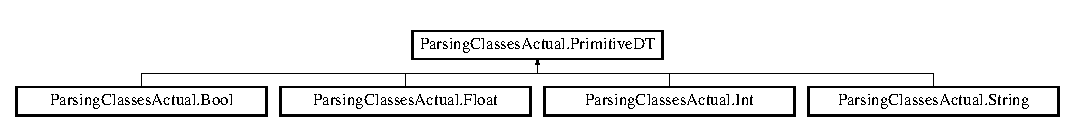
\includegraphics[height=1.327014cm]{class_parsing_classes_actual_1_1_primitive_d_t}
\end{center}
\end{figure}
\subsection*{Public Member Functions}
\begin{DoxyCompactItemize}
\item 
\mbox{\Hypertarget{class_parsing_classes_actual_1_1_primitive_d_t_a2304320d29f6a8dc8ae980daf77f2f05}\label{class_parsing_classes_actual_1_1_primitive_d_t_a2304320d29f6a8dc8ae980daf77f2f05}} 
def \hyperlink{class_parsing_classes_actual_1_1_primitive_d_t_a2304320d29f6a8dc8ae980daf77f2f05}{\+\_\+\+\_\+init\+\_\+\+\_\+} (self, value)
\begin{DoxyCompactList}\small\item\em The constructor which takes a value and stores it. \end{DoxyCompactList}\item 
\mbox{\Hypertarget{class_parsing_classes_actual_1_1_primitive_d_t_a39857bf656def22c6270a26804e1d7aa}\label{class_parsing_classes_actual_1_1_primitive_d_t_a39857bf656def22c6270a26804e1d7aa}} 
def \hyperlink{class_parsing_classes_actual_1_1_primitive_d_t_a39857bf656def22c6270a26804e1d7aa}{eval} (self)
\begin{DoxyCompactList}\small\item\em the evaluate function which returns the value \end{DoxyCompactList}\item 
def \hyperlink{class_parsing_classes_actual_1_1_primitive_d_t_ac6dd10edd29b85354b53ad165f5704d1}{update} (self, val)
\begin{DoxyCompactList}\small\item\em The update function which updates the value stored. \end{DoxyCompactList}\end{DoxyCompactItemize}
\subsection*{Public Attributes}
\begin{DoxyCompactItemize}
\item 
\mbox{\Hypertarget{class_parsing_classes_actual_1_1_primitive_d_t_a5068a462424619a605aaa95ad6e133ea}\label{class_parsing_classes_actual_1_1_primitive_d_t_a5068a462424619a605aaa95ad6e133ea}} 
{\bfseries value}
\end{DoxyCompactItemize}


\subsection{Detailed Description}
The basic class which stores values of basic data structures like numbers,strings and boolean. 

Some of the operations are similar for all datatypes, which have been inherired from \hyperlink{class_parsing_classes_actual_1_1_primitive_d_t}{Primitive\+DT}. basic datatypes that appear as it is in an expression are stored as subclass of primitive\+DT. eg. x=7+x; 7 is stored as primitive DT 

\subsection{Member Function Documentation}
\mbox{\Hypertarget{class_parsing_classes_actual_1_1_primitive_d_t_ac6dd10edd29b85354b53ad165f5704d1}\label{class_parsing_classes_actual_1_1_primitive_d_t_ac6dd10edd29b85354b53ad165f5704d1}} 
\index{Parsing\+Classes\+Actual\+::\+Primitive\+DT@{Parsing\+Classes\+Actual\+::\+Primitive\+DT}!update@{update}}
\index{update@{update}!Parsing\+Classes\+Actual\+::\+Primitive\+DT@{Parsing\+Classes\+Actual\+::\+Primitive\+DT}}
\subsubsection{\texorpdfstring{update()}{update()}}
{\footnotesize\ttfamily def Parsing\+Classes\+Actual.\+Primitive\+D\+T.\+update (\begin{DoxyParamCaption}\item[{}]{self,  }\item[{}]{val }\end{DoxyParamCaption})}



The update function which updates the value stored. 


\begin{DoxyParams}{Parameters}
{\em val} & The value to which it is to be updated \\
\hline
\end{DoxyParams}


The documentation for this class was generated from the following file\+:\begin{DoxyCompactItemize}
\item 
Parsing\+Classes\+Actual.\+py\end{DoxyCompactItemize}

\hypertarget{classparser_classes_1_1_primitive_d_t}{}\section{parser\+Classes.\+Primitive\+DT Class Reference}
\label{classparser_classes_1_1_primitive_d_t}\index{parser\+Classes.\+Primitive\+DT@{parser\+Classes.\+Primitive\+DT}}
Inheritance diagram for parser\+Classes.\+Primitive\+DT\+:\begin{figure}[H]
\begin{center}
\leavevmode
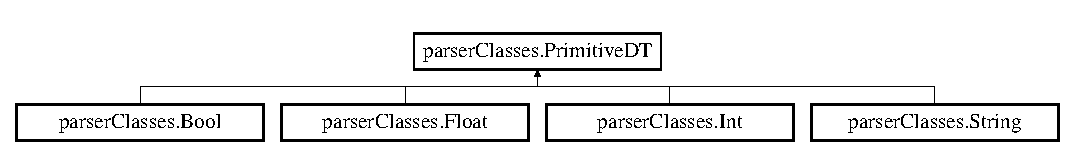
\includegraphics[height=1.656805cm]{classparser_classes_1_1_primitive_d_t}
\end{center}
\end{figure}
\subsection*{Public Member Functions}
\begin{DoxyCompactItemize}
\item 
\mbox{\Hypertarget{classparser_classes_1_1_primitive_d_t_afc7a88a3500def7e2831c94385b822e3}\label{classparser_classes_1_1_primitive_d_t_afc7a88a3500def7e2831c94385b822e3}} 
def {\bfseries \+\_\+\+\_\+init\+\_\+\+\_\+} (self, value)
\item 
\mbox{\Hypertarget{classparser_classes_1_1_primitive_d_t_a4b0a4891bc06d83090e2dde406114214}\label{classparser_classes_1_1_primitive_d_t_a4b0a4891bc06d83090e2dde406114214}} 
def {\bfseries eval} (self)
\item 
\mbox{\Hypertarget{classparser_classes_1_1_primitive_d_t_ad52adc67041de2a7abfe4c25c0b0558d}\label{classparser_classes_1_1_primitive_d_t_ad52adc67041de2a7abfe4c25c0b0558d}} 
def {\bfseries update} (self, val)
\end{DoxyCompactItemize}
\subsection*{Public Attributes}
\begin{DoxyCompactItemize}
\item 
\mbox{\Hypertarget{classparser_classes_1_1_primitive_d_t_a2f2bc9ba2df4e0db223f44eef3f2c162}\label{classparser_classes_1_1_primitive_d_t_a2f2bc9ba2df4e0db223f44eef3f2c162}} 
{\bfseries value}
\end{DoxyCompactItemize}


The documentation for this class was generated from the following file\+:\begin{DoxyCompactItemize}
\item 
parser\+Classes.\+py\end{DoxyCompactItemize}

\hypertarget{class_queue_1_1_queue}{}\section{Queue.\+Queue Class Reference}
\label{class_queue_1_1_queue}\index{Queue.\+Queue@{Queue.\+Queue}}


Pre-\/defined data structure to represent a Double sided queue.  


\subsection*{Public Member Functions}
\begin{DoxyCompactItemize}
\item 
def \hyperlink{class_queue_1_1_queue_a775357405d27ad4bdf5ed097bee49665}{\+\_\+\+\_\+init\+\_\+\+\_\+} (self, x, y, model\+Type, name)
\begin{DoxyCompactList}\small\item\em Constructor for the class. \end{DoxyCompactList}\item 
\mbox{\Hypertarget{class_queue_1_1_queue_a1472c6353f40c911d09da436ce8b2baa}\label{class_queue_1_1_queue_a1472c6353f40c911d09da436ce8b2baa}} 
def \hyperlink{class_queue_1_1_queue_a1472c6353f40c911d09da436ce8b2baa}{empty} (self)
\begin{DoxyCompactList}\small\item\em Function which returns true if the queue is empty and false otherwise. \end{DoxyCompactList}\item 
\mbox{\Hypertarget{class_queue_1_1_queue_a478b93022acfd9225f15868f5eda0410}\label{class_queue_1_1_queue_a478b93022acfd9225f15868f5eda0410}} 
def \hyperlink{class_queue_1_1_queue_a478b93022acfd9225f15868f5eda0410}{size} (self)
\begin{DoxyCompactList}\small\item\em Function which returns the size of the queue. \end{DoxyCompactList}\item 
def \hyperlink{class_queue_1_1_queue_a6333268eb174c6fda6f9574e951710b2}{push\+Back} (self, val)
\begin{DoxyCompactList}\small\item\em Function which pushes a new node to the end of the queue. \end{DoxyCompactList}\item 
def \hyperlink{class_queue_1_1_queue_a17b55e82b5a8db529ff6a23a6b14bb03}{push\+Front} (self, val)
\begin{DoxyCompactList}\small\item\em Function to push a node to the front of the queue. \end{DoxyCompactList}\item 
def \hyperlink{class_queue_1_1_queue_a7d3ec12e83314c6a109e8403b9250c30}{front} (self)
\begin{DoxyCompactList}\small\item\em Function to return the element that is at the front of the queue. \end{DoxyCompactList}\item 
def \hyperlink{class_queue_1_1_queue_ab49a295f4ebc449e5830119085493614}{back} (self)
\begin{DoxyCompactList}\small\item\em Function to return the element at the back of the queue. \end{DoxyCompactList}\item 
def \hyperlink{class_queue_1_1_queue_aa2cd3a51ee6600ca226f7c43623d6ede}{pop\+Front} (self)
\begin{DoxyCompactList}\small\item\em Function to pop the element at the front of the queue. \end{DoxyCompactList}\item 
def \hyperlink{class_queue_1_1_queue_a192c71ff5839f8b1970976eefaaec777}{pop\+Back} (self)
\begin{DoxyCompactList}\small\item\em Function to pop the element at the back of the queue. \end{DoxyCompactList}\item 
def \hyperlink{class_queue_1_1_queue_ac384b9efaf5e8d9b1b7a34183062468c}{delete} (self)
\begin{DoxyCompactList}\small\item\em Function to undraw all the graphics related to the queue and then delete all the data members. \end{DoxyCompactList}\end{DoxyCompactItemize}
\subsection*{Public Attributes}
\begin{DoxyCompactItemize}
\item 
\mbox{\Hypertarget{class_queue_1_1_queue_ab4a0969d72be3d0fb08e02a33a985640}\label{class_queue_1_1_queue_ab4a0969d72be3d0fb08e02a33a985640}} 
{\bfseries starting\+Point}
\item 
\mbox{\Hypertarget{class_queue_1_1_queue_a692f39189799e9729806e99e59dff97d}\label{class_queue_1_1_queue_a692f39189799e9729806e99e59dff97d}} 
{\bfseries name\+Text}
\item 
\mbox{\Hypertarget{class_queue_1_1_queue_abd20d1d760a1275d551b4eebd709c110}\label{class_queue_1_1_queue_abd20d1d760a1275d551b4eebd709c110}} 
{\bfseries name}
\item 
\mbox{\Hypertarget{class_queue_1_1_queue_a1e239f58b74790246aeec49e81f9052d}\label{class_queue_1_1_queue_a1e239f58b74790246aeec49e81f9052d}} 
{\bfseries type}
\item 
\mbox{\Hypertarget{class_queue_1_1_queue_a9a2010a83cf36c0d23c2d90396cd3796}\label{class_queue_1_1_queue_a9a2010a83cf36c0d23c2d90396cd3796}} 
{\bfseries head}
\item 
\mbox{\Hypertarget{class_queue_1_1_queue_a70d68f8c761879b479bac48d291c0671}\label{class_queue_1_1_queue_a70d68f8c761879b479bac48d291c0671}} 
{\bfseries tail}
\item 
\mbox{\Hypertarget{class_queue_1_1_queue_a88cc9ea7e3c5ad6afb3635b1f493bfcd}\label{class_queue_1_1_queue_a88cc9ea7e3c5ad6afb3635b1f493bfcd}} 
{\bfseries size}
\item 
\mbox{\Hypertarget{class_queue_1_1_queue_a13809fa8a00047c724274dc36d7255e0}\label{class_queue_1_1_queue_a13809fa8a00047c724274dc36d7255e0}} 
{\bfseries text}
\end{DoxyCompactItemize}


\subsection{Detailed Description}
Pre-\/defined data structure to represent a Double sided queue. 

Contians all the data members and member functions to represent a standard singly linked list Abstract Data Type In addition to this, it contains all the needed data members and functions to represent the data structure on the canvas. Usual functions have been modified to allow for the required changes to the graph as well. 

\subsection{Constructor \& Destructor Documentation}
\mbox{\Hypertarget{class_queue_1_1_queue_a775357405d27ad4bdf5ed097bee49665}\label{class_queue_1_1_queue_a775357405d27ad4bdf5ed097bee49665}} 
\index{Queue\+::\+Queue@{Queue\+::\+Queue}!\+\_\+\+\_\+init\+\_\+\+\_\+@{\+\_\+\+\_\+init\+\_\+\+\_\+}}
\index{\+\_\+\+\_\+init\+\_\+\+\_\+@{\+\_\+\+\_\+init\+\_\+\+\_\+}!Queue\+::\+Queue@{Queue\+::\+Queue}}
\subsubsection{\texorpdfstring{\+\_\+\+\_\+init\+\_\+\+\_\+()}{\_\_init\_\_()}}
{\footnotesize\ttfamily def Queue.\+Queue.\+\_\+\+\_\+init\+\_\+\+\_\+ (\begin{DoxyParamCaption}\item[{}]{self,  }\item[{}]{x,  }\item[{}]{y,  }\item[{}]{model\+Type,  }\item[{}]{name }\end{DoxyParamCaption})}



Constructor for the class. 


\begin{DoxyParams}{Parameters}
{\em x} & -\/ the x coordinate of the rightmost corner of the queue. \\
\hline
{\em y} & -\/ the y coordinate of the rightmost corner of the queue. \\
\hline
{\em model\+Type} & -\/ An object of the type to be stored in the queue, to ensure that all elements in the list are of the same type as in C++ \\
\hline
{\em name} & -\/ The name given by the user to an instance of this class. \\
\hline
\end{DoxyParams}


\subsection{Member Function Documentation}
\mbox{\Hypertarget{class_queue_1_1_queue_ab49a295f4ebc449e5830119085493614}\label{class_queue_1_1_queue_ab49a295f4ebc449e5830119085493614}} 
\index{Queue\+::\+Queue@{Queue\+::\+Queue}!back@{back}}
\index{back@{back}!Queue\+::\+Queue@{Queue\+::\+Queue}}
\subsubsection{\texorpdfstring{back()}{back()}}
{\footnotesize\ttfamily def Queue.\+Queue.\+back (\begin{DoxyParamCaption}\item[{}]{self }\end{DoxyParamCaption})}



Function to return the element at the back of the queue. 

It raises an error if the queue is empty. \mbox{\Hypertarget{class_queue_1_1_queue_ac384b9efaf5e8d9b1b7a34183062468c}\label{class_queue_1_1_queue_ac384b9efaf5e8d9b1b7a34183062468c}} 
\index{Queue\+::\+Queue@{Queue\+::\+Queue}!delete@{delete}}
\index{delete@{delete}!Queue\+::\+Queue@{Queue\+::\+Queue}}
\subsubsection{\texorpdfstring{delete()}{delete()}}
{\footnotesize\ttfamily def Queue.\+Queue.\+delete (\begin{DoxyParamCaption}\item[{}]{self }\end{DoxyParamCaption})}



Function to undraw all the graphics related to the queue and then delete all the data members. 

\mbox{\Hypertarget{class_queue_1_1_queue_a7d3ec12e83314c6a109e8403b9250c30}\label{class_queue_1_1_queue_a7d3ec12e83314c6a109e8403b9250c30}} 
\index{Queue\+::\+Queue@{Queue\+::\+Queue}!front@{front}}
\index{front@{front}!Queue\+::\+Queue@{Queue\+::\+Queue}}
\subsubsection{\texorpdfstring{front()}{front()}}
{\footnotesize\ttfamily def Queue.\+Queue.\+front (\begin{DoxyParamCaption}\item[{}]{self }\end{DoxyParamCaption})}



Function to return the element that is at the front of the queue. 

It raises an error if the queue is empty. \mbox{\Hypertarget{class_queue_1_1_queue_a192c71ff5839f8b1970976eefaaec777}\label{class_queue_1_1_queue_a192c71ff5839f8b1970976eefaaec777}} 
\index{Queue\+::\+Queue@{Queue\+::\+Queue}!pop\+Back@{pop\+Back}}
\index{pop\+Back@{pop\+Back}!Queue\+::\+Queue@{Queue\+::\+Queue}}
\subsubsection{\texorpdfstring{pop\+Back()}{popBack()}}
{\footnotesize\ttfamily def Queue.\+Queue.\+pop\+Back (\begin{DoxyParamCaption}\item[{}]{self }\end{DoxyParamCaption})}



Function to pop the element at the back of the queue. 

If the queue is empty, then raise an error\+: \mbox{\Hypertarget{class_queue_1_1_queue_aa2cd3a51ee6600ca226f7c43623d6ede}\label{class_queue_1_1_queue_aa2cd3a51ee6600ca226f7c43623d6ede}} 
\index{Queue\+::\+Queue@{Queue\+::\+Queue}!pop\+Front@{pop\+Front}}
\index{pop\+Front@{pop\+Front}!Queue\+::\+Queue@{Queue\+::\+Queue}}
\subsubsection{\texorpdfstring{pop\+Front()}{popFront()}}
{\footnotesize\ttfamily def Queue.\+Queue.\+pop\+Front (\begin{DoxyParamCaption}\item[{}]{self }\end{DoxyParamCaption})}



Function to pop the element at the front of the queue. 

If queue is empty, then raise an error\+: \mbox{\Hypertarget{class_queue_1_1_queue_a6333268eb174c6fda6f9574e951710b2}\label{class_queue_1_1_queue_a6333268eb174c6fda6f9574e951710b2}} 
\index{Queue\+::\+Queue@{Queue\+::\+Queue}!push\+Back@{push\+Back}}
\index{push\+Back@{push\+Back}!Queue\+::\+Queue@{Queue\+::\+Queue}}
\subsubsection{\texorpdfstring{push\+Back()}{pushBack()}}
{\footnotesize\ttfamily def Queue.\+Queue.\+push\+Back (\begin{DoxyParamCaption}\item[{}]{self,  }\item[{}]{val }\end{DoxyParamCaption})}



Function which pushes a new node to the end of the queue. 


\begin{DoxyParams}{Parameters}
{\em val} & -\/ the value to be stored in the node that is to be pushed. \\
\hline
\end{DoxyParams}
\mbox{\Hypertarget{class_queue_1_1_queue_a17b55e82b5a8db529ff6a23a6b14bb03}\label{class_queue_1_1_queue_a17b55e82b5a8db529ff6a23a6b14bb03}} 
\index{Queue\+::\+Queue@{Queue\+::\+Queue}!push\+Front@{push\+Front}}
\index{push\+Front@{push\+Front}!Queue\+::\+Queue@{Queue\+::\+Queue}}
\subsubsection{\texorpdfstring{push\+Front()}{pushFront()}}
{\footnotesize\ttfamily def Queue.\+Queue.\+push\+Front (\begin{DoxyParamCaption}\item[{}]{self,  }\item[{}]{val }\end{DoxyParamCaption})}



Function to push a node to the front of the queue. 


\begin{DoxyParams}{Parameters}
{\em val} & -\/ the value to be stored in the node that is to be pushed. \\
\hline
\end{DoxyParams}


The documentation for this class was generated from the following file\+:\begin{DoxyCompactItemize}
\item 
Queue.\+py\end{DoxyCompactItemize}

\hypertarget{class_queue_1_1_queue_node}{}\section{Queue.\+Queue\+Node Class Reference}
\label{class_queue_1_1_queue_node}\index{Queue.\+Queue\+Node@{Queue.\+Queue\+Node}}
\subsection*{Public Member Functions}
\begin{DoxyCompactItemize}
\item 
def {\bfseries \+\_\+\+\_\+init\+\_\+\+\_\+} (self, x, y, val, nxt)\hypertarget{class_queue_1_1_queue_node_acfe34780ae926af46ebe32a58c8e030c}{}\label{class_queue_1_1_queue_node_acfe34780ae926af46ebe32a58c8e030c}

\item 
def {\bfseries change\+Color} (self, color)\hypertarget{class_queue_1_1_queue_node_a97a3e71ba6dddf6a6d40d4222402238b}{}\label{class_queue_1_1_queue_node_a97a3e71ba6dddf6a6d40d4222402238b}

\item 
def {\bfseries shift\+Ahead} (self)\hypertarget{class_queue_1_1_queue_node_a71dbaccc8320cb100d14fcf8c8764c83}{}\label{class_queue_1_1_queue_node_a71dbaccc8320cb100d14fcf8c8764c83}

\item 
def {\bfseries shift\+Behind} (self)\hypertarget{class_queue_1_1_queue_node_ac4f2637c989e8d98c5bf20ce9481dce4}{}\label{class_queue_1_1_queue_node_ac4f2637c989e8d98c5bf20ce9481dce4}

\item 
def {\bfseries delete} (self)\hypertarget{class_queue_1_1_queue_node_af50c356dd13964a0378e13034eec53ca}{}\label{class_queue_1_1_queue_node_af50c356dd13964a0378e13034eec53ca}

\end{DoxyCompactItemize}
\subsection*{Public Attributes}
\begin{DoxyCompactItemize}
\item 
{\bfseries data}\hypertarget{class_queue_1_1_queue_node_aa9448b7ef31d8dd61adb504ccf7b1c44}{}\label{class_queue_1_1_queue_node_aa9448b7ef31d8dd61adb504ccf7b1c44}

\item 
{\bfseries next}\hypertarget{class_queue_1_1_queue_node_a736cdbadd2c72609a9964dd149054db0}{}\label{class_queue_1_1_queue_node_a736cdbadd2c72609a9964dd149054db0}

\item 
{\bfseries circle}\hypertarget{class_queue_1_1_queue_node_ac113a4d52ea51f0c6fcb65b30e6e0761}{}\label{class_queue_1_1_queue_node_ac113a4d52ea51f0c6fcb65b30e6e0761}

\item 
{\bfseries text}\hypertarget{class_queue_1_1_queue_node_a3e732e4728a03dd3c333782519efb320}{}\label{class_queue_1_1_queue_node_a3e732e4728a03dd3c333782519efb320}

\item 
{\bfseries arrow}\hypertarget{class_queue_1_1_queue_node_a762acb0de1bf2321d766376c383ffbb0}{}\label{class_queue_1_1_queue_node_a762acb0de1bf2321d766376c383ffbb0}

\end{DoxyCompactItemize}


The documentation for this class was generated from the following file\+:\begin{DoxyCompactItemize}
\item 
Queue.\+py\end{DoxyCompactItemize}

\hypertarget{classgraphics_1_1_rectangle}{}\section{graphics.\+Rectangle Class Reference}
\label{classgraphics_1_1_rectangle}\index{graphics.\+Rectangle@{graphics.\+Rectangle}}
Inheritance diagram for graphics.\+Rectangle\+:\begin{figure}[H]
\begin{center}
\leavevmode
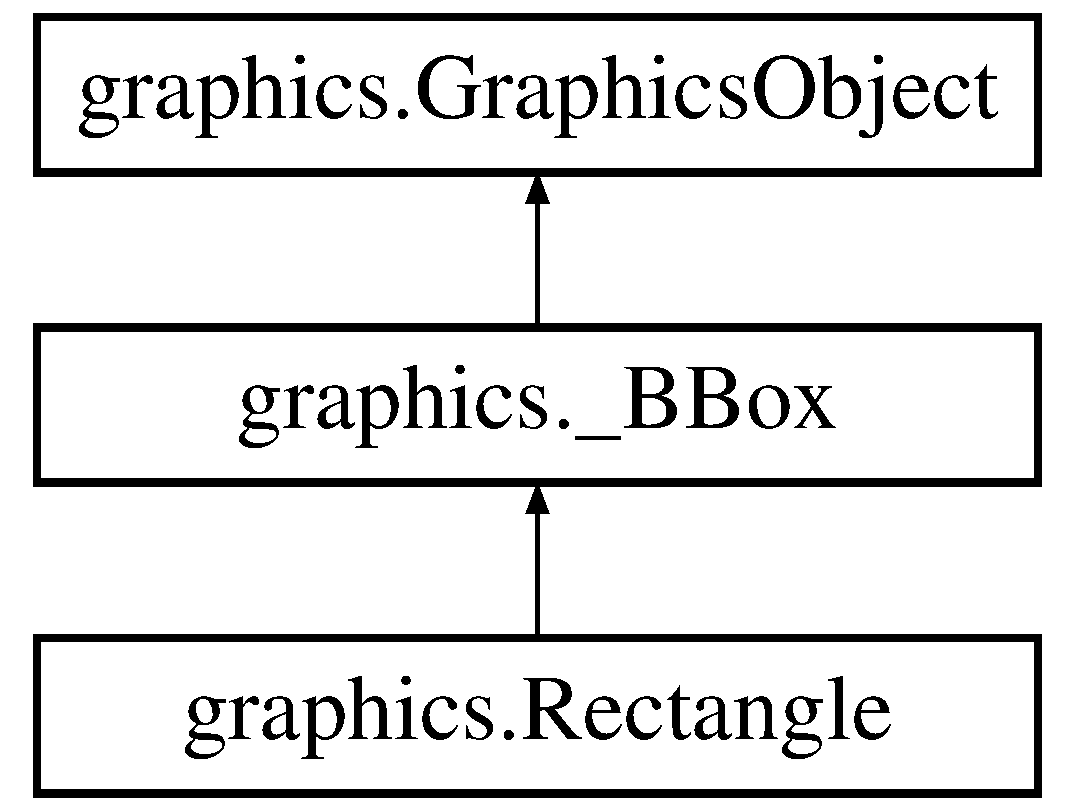
\includegraphics[height=3.000000cm]{classgraphics_1_1_rectangle}
\end{center}
\end{figure}
\subsection*{Public Member Functions}
\begin{DoxyCompactItemize}
\item 
\mbox{\Hypertarget{classgraphics_1_1_rectangle_a691f947134b1fc54443c55aa9d6214c5}\label{classgraphics_1_1_rectangle_a691f947134b1fc54443c55aa9d6214c5}} 
def {\bfseries \+\_\+\+\_\+init\+\_\+\+\_\+} (self, p1, p2)
\item 
\mbox{\Hypertarget{classgraphics_1_1_rectangle_af16c7826cc639912ec3ef819f6ac467e}\label{classgraphics_1_1_rectangle_af16c7826cc639912ec3ef819f6ac467e}} 
def {\bfseries \+\_\+\+\_\+repr\+\_\+\+\_\+} (self)
\item 
\mbox{\Hypertarget{classgraphics_1_1_rectangle_aaffe12a1bc2f5fc5ff221c909d2fb583}\label{classgraphics_1_1_rectangle_aaffe12a1bc2f5fc5ff221c909d2fb583}} 
def {\bfseries clone} (self)
\end{DoxyCompactItemize}
\subsection*{Additional Inherited Members}


The documentation for this class was generated from the following file\+:\begin{DoxyCompactItemize}
\item 
graphics.\+py\end{DoxyCompactItemize}

\hypertarget{classparser_classes_1_1_return}{}\section{parser\+Classes.\+Return Class Reference}
\label{classparser_classes_1_1_return}\index{parser\+Classes.\+Return@{parser\+Classes.\+Return}}
\subsection*{Public Member Functions}
\begin{DoxyCompactItemize}
\item 
def {\bfseries \+\_\+\+\_\+init\+\_\+\+\_\+} (self, exp=\hyperlink{classparser_classes_1_1_string}{String}())\hypertarget{classparser_classes_1_1_return_a3034474866e17be4742096ed2434b80d}{}\label{classparser_classes_1_1_return_a3034474866e17be4742096ed2434b80d}

\item 
def {\bfseries exec} (self)\hypertarget{classparser_classes_1_1_return_a0d771079b3f705e980d25c2a4d3c9bd9}{}\label{classparser_classes_1_1_return_a0d771079b3f705e980d25c2a4d3c9bd9}

\end{DoxyCompactItemize}
\subsection*{Public Attributes}
\begin{DoxyCompactItemize}
\item 
{\bfseries exp}\hypertarget{classparser_classes_1_1_return_a2b35e75cdff0a6fbd98f539a679e7848}{}\label{classparser_classes_1_1_return_a2b35e75cdff0a6fbd98f539a679e7848}

\end{DoxyCompactItemize}


The documentation for this class was generated from the following file\+:\begin{DoxyCompactItemize}
\item 
parser\+Classes.\+py\end{DoxyCompactItemize}

\hypertarget{class_parsing_classes_actual_1_1_return}{}\section{Parsing\+Classes\+Actual.\+Return Class Reference}
\label{class_parsing_classes_actual_1_1_return}\index{Parsing\+Classes\+Actual.\+Return@{Parsing\+Classes\+Actual.\+Return}}
\subsection*{Public Member Functions}
\begin{DoxyCompactItemize}
\item 
def {\bfseries \+\_\+\+\_\+init\+\_\+\+\_\+} (self, exp, snippet)\hypertarget{class_parsing_classes_actual_1_1_return_af8d6700c68272fc7a9f66befd743e547}{}\label{class_parsing_classes_actual_1_1_return_af8d6700c68272fc7a9f66befd743e547}

\item 
def {\bfseries exec} (self)\hypertarget{class_parsing_classes_actual_1_1_return_a0abe605098c54c3c29e865a40efb58ce}{}\label{class_parsing_classes_actual_1_1_return_a0abe605098c54c3c29e865a40efb58ce}

\end{DoxyCompactItemize}
\subsection*{Public Attributes}
\begin{DoxyCompactItemize}
\item 
{\bfseries exp}\hypertarget{class_parsing_classes_actual_1_1_return_a49d43bb82d1a79d3f181dbc8cf159f09}{}\label{class_parsing_classes_actual_1_1_return_a49d43bb82d1a79d3f181dbc8cf159f09}

\item 
{\bfseries snippet}\hypertarget{class_parsing_classes_actual_1_1_return_af4603fca7bfda265c24ce85e21f1c21a}{}\label{class_parsing_classes_actual_1_1_return_af4603fca7bfda265c24ce85e21f1c21a}

\end{DoxyCompactItemize}


The documentation for this class was generated from the following file\+:\begin{DoxyCompactItemize}
\item 
Parsing\+Classes\+Actual.\+py\end{DoxyCompactItemize}

\hypertarget{classheaders_for_data_structures_1_1right_arrow}{}\section{headers\+For\+Data\+Structures.\+right\+Arrow Class Reference}
\label{classheaders_for_data_structures_1_1right_arrow}\index{headers\+For\+Data\+Structures.\+right\+Arrow@{headers\+For\+Data\+Structures.\+right\+Arrow}}


Class contaning arrows to make a pointer between objects on the canvas  


\subsection*{Public Member Functions}
\begin{DoxyCompactItemize}
\item 
\mbox{\Hypertarget{classheaders_for_data_structures_1_1right_arrow_a0d53d254a151ec5db5331c8a6afd36c0}\label{classheaders_for_data_structures_1_1right_arrow_a0d53d254a151ec5db5331c8a6afd36c0}} 
def \hyperlink{classheaders_for_data_structures_1_1right_arrow_a0d53d254a151ec5db5331c8a6afd36c0}{\+\_\+\+\_\+init\+\_\+\+\_\+} (self, x, y)
\begin{DoxyCompactList}\small\item\em The constructor, with the coordinates of where to make the arrow. \end{DoxyCompactList}\item 
\mbox{\Hypertarget{classheaders_for_data_structures_1_1right_arrow_a0ab3e6bded6c7acb0c4dc9ba61d7ac31}\label{classheaders_for_data_structures_1_1right_arrow_a0ab3e6bded6c7acb0c4dc9ba61d7ac31}} 
def \hyperlink{classheaders_for_data_structures_1_1right_arrow_a0ab3e6bded6c7acb0c4dc9ba61d7ac31}{draw} (self)
\begin{DoxyCompactList}\small\item\em Function to actually draw the arrow on the canvas. \end{DoxyCompactList}\item 
\mbox{\Hypertarget{classheaders_for_data_structures_1_1right_arrow_a0a5c65179b5c92ce3d79d6f1c1678b5b}\label{classheaders_for_data_structures_1_1right_arrow_a0a5c65179b5c92ce3d79d6f1c1678b5b}} 
def \hyperlink{classheaders_for_data_structures_1_1right_arrow_a0a5c65179b5c92ce3d79d6f1c1678b5b}{undraw} (self)
\begin{DoxyCompactList}\small\item\em Function to undraw the arrow. \end{DoxyCompactList}\item 
\mbox{\Hypertarget{classheaders_for_data_structures_1_1right_arrow_a3a9f5debd35ed66cc2b3a7c64397d530}\label{classheaders_for_data_structures_1_1right_arrow_a3a9f5debd35ed66cc2b3a7c64397d530}} 
def \hyperlink{classheaders_for_data_structures_1_1right_arrow_a3a9f5debd35ed66cc2b3a7c64397d530}{shift\+Ahead} (self)
\begin{DoxyCompactList}\small\item\em Function to shift the arrow ahead so that if the elements of a lsit are deleted, we can update the structure. \end{DoxyCompactList}\item 
\mbox{\Hypertarget{classheaders_for_data_structures_1_1right_arrow_a3e9d01ac5c06f2c21facde8562303d8f}\label{classheaders_for_data_structures_1_1right_arrow_a3e9d01ac5c06f2c21facde8562303d8f}} 
def \hyperlink{classheaders_for_data_structures_1_1right_arrow_a3e9d01ac5c06f2c21facde8562303d8f}{shift\+Behind} (self)
\begin{DoxyCompactList}\small\item\em Function to shift the arrow behind so that if the elements of a list are deleted, we can update the structure. \end{DoxyCompactList}\item 
\mbox{\Hypertarget{classheaders_for_data_structures_1_1right_arrow_a70f3a761d27bd00ff60b71bd4457752d}\label{classheaders_for_data_structures_1_1right_arrow_a70f3a761d27bd00ff60b71bd4457752d}} 
def \hyperlink{classheaders_for_data_structures_1_1right_arrow_a70f3a761d27bd00ff60b71bd4457752d}{shift\+In\+Queue} (self)
\begin{DoxyCompactList}\small\item\em Function to move the arrow when the queue is updated. \end{DoxyCompactList}\item 
\mbox{\Hypertarget{classheaders_for_data_structures_1_1right_arrow_a89971076429e090ee142a0ac82dd51ce}\label{classheaders_for_data_structures_1_1right_arrow_a89971076429e090ee142a0ac82dd51ce}} 
def \hyperlink{classheaders_for_data_structures_1_1right_arrow_a89971076429e090ee142a0ac82dd51ce}{shift\+Behind\+In\+Queue} (self)
\begin{DoxyCompactList}\small\item\em Function to move the arrow behind in the queue when an element is added to the front of the queue. \end{DoxyCompactList}\end{DoxyCompactItemize}
\subsection*{Public Attributes}
\begin{DoxyCompactItemize}
\item 
\mbox{\Hypertarget{classheaders_for_data_structures_1_1right_arrow_aee6de10c02c9ea41f85dda3608bc2c29}\label{classheaders_for_data_structures_1_1right_arrow_aee6de10c02c9ea41f85dda3608bc2c29}} 
{\bfseries line}
\item 
\mbox{\Hypertarget{classheaders_for_data_structures_1_1right_arrow_a8d9040aee6f54367b956a1af7aec6401}\label{classheaders_for_data_structures_1_1right_arrow_a8d9040aee6f54367b956a1af7aec6401}} 
{\bfseries arrowhead1}
\item 
\mbox{\Hypertarget{classheaders_for_data_structures_1_1right_arrow_a057c3637cb94f18827aa4ffa86dd3355}\label{classheaders_for_data_structures_1_1right_arrow_a057c3637cb94f18827aa4ffa86dd3355}} 
{\bfseries arrowhead2}
\end{DoxyCompactItemize}


\subsection{Detailed Description}
Class contaning arrows to make a pointer between objects on the canvas 

The documentation for this class was generated from the following file\+:\begin{DoxyCompactItemize}
\item 
headers\+For\+Data\+Structures.\+py\end{DoxyCompactItemize}

\hypertarget{class_parsing_classes_actual_1_1_simplex}{}\section{Parsing\+Classes\+Actual.\+Simplex Class Reference}
\label{class_parsing_classes_actual_1_1_simplex}\index{Parsing\+Classes\+Actual.\+Simplex@{Parsing\+Classes\+Actual.\+Simplex}}
\subsection*{Public Member Functions}
\begin{DoxyCompactItemize}
\item 
def {\bfseries \+\_\+\+\_\+init\+\_\+\+\_\+} (self)\hypertarget{class_parsing_classes_actual_1_1_simplex_a4f09c613fb672e206b532b5abb96576e}{}\label{class_parsing_classes_actual_1_1_simplex_a4f09c613fb672e206b532b5abb96576e}

\item 
def {\bfseries add\+Element} (self, element)\hypertarget{class_parsing_classes_actual_1_1_simplex_a5c2423d5d737475748de577076863d57}{}\label{class_parsing_classes_actual_1_1_simplex_a5c2423d5d737475748de577076863d57}

\item 
def {\bfseries eval} (self)\hypertarget{class_parsing_classes_actual_1_1_simplex_a5955c7802478a8ed5e31a0264a32ac41}{}\label{class_parsing_classes_actual_1_1_simplex_a5955c7802478a8ed5e31a0264a32ac41}

\end{DoxyCompactItemize}
\subsection*{Public Attributes}
\begin{DoxyCompactItemize}
\item 
{\bfseries elements}\hypertarget{class_parsing_classes_actual_1_1_simplex_ae4c51bf50905e135df64c996c63b1247}{}\label{class_parsing_classes_actual_1_1_simplex_ae4c51bf50905e135df64c996c63b1247}

\end{DoxyCompactItemize}


The documentation for this class was generated from the following file\+:\begin{DoxyCompactItemize}
\item 
Parsing\+Classes\+Actual.\+py\end{DoxyCompactItemize}

\hypertarget{classparser_classes_1_1_simplex}{}\section{parser\+Classes.\+Simplex Class Reference}
\label{classparser_classes_1_1_simplex}\index{parser\+Classes.\+Simplex@{parser\+Classes.\+Simplex}}
\subsection*{Public Member Functions}
\begin{DoxyCompactItemize}
\item 
\mbox{\Hypertarget{classparser_classes_1_1_simplex_ae0d244c9cd73a6ccb9fe38a5e2045818}\label{classparser_classes_1_1_simplex_ae0d244c9cd73a6ccb9fe38a5e2045818}} 
def {\bfseries \+\_\+\+\_\+init\+\_\+\+\_\+} (self)
\item 
\mbox{\Hypertarget{classparser_classes_1_1_simplex_ab4f047be45ac43f11b9fb18691ca1413}\label{classparser_classes_1_1_simplex_ab4f047be45ac43f11b9fb18691ca1413}} 
def {\bfseries add\+Element} (self, element)
\item 
\mbox{\Hypertarget{classparser_classes_1_1_simplex_adbbb7c22025953fc0690e4bcd22ce4cc}\label{classparser_classes_1_1_simplex_adbbb7c22025953fc0690e4bcd22ce4cc}} 
def {\bfseries eval} (self)
\end{DoxyCompactItemize}
\subsection*{Public Attributes}
\begin{DoxyCompactItemize}
\item 
\mbox{\Hypertarget{classparser_classes_1_1_simplex_a20765598c2e5bc570cc0ea135920d4ea}\label{classparser_classes_1_1_simplex_a20765598c2e5bc570cc0ea135920d4ea}} 
{\bfseries elements}
\end{DoxyCompactItemize}


The documentation for this class was generated from the following file\+:\begin{DoxyCompactItemize}
\item 
parser\+Classes.\+py\end{DoxyCompactItemize}

\hypertarget{class_singly_linked_list_1_1_singly_linked_list}{}\section{Singly\+Linked\+List.\+Singly\+Linked\+List Class Reference}
\label{class_singly_linked_list_1_1_singly_linked_list}\index{Singly\+Linked\+List.\+Singly\+Linked\+List@{Singly\+Linked\+List.\+Singly\+Linked\+List}}


Pre-\/defined data structure to represent a Singly Linked List.  


\subsection*{Public Member Functions}
\begin{DoxyCompactItemize}
\item 
def \hyperlink{class_singly_linked_list_1_1_singly_linked_list_a2e508ae2b37528ee587753422068f144}{\+\_\+\+\_\+init\+\_\+\+\_\+} (self, x, y, model\+Type, name)
\begin{DoxyCompactList}\small\item\em Constructor for the class. \end{DoxyCompactList}\item 
def \hyperlink{class_singly_linked_list_1_1_singly_linked_list_a96f6f50cf9bed918fe1f5248c1649f0c}{size} (self)
\begin{DoxyCompactList}\small\item\em Return the number of elements in the list -\/ no graphical changes. \end{DoxyCompactList}\item 
\mbox{\Hypertarget{class_singly_linked_list_1_1_singly_linked_list_af6f27944245081ce67217ffc2a875a76}\label{class_singly_linked_list_1_1_singly_linked_list_af6f27944245081ce67217ffc2a875a76}} 
def \hyperlink{class_singly_linked_list_1_1_singly_linked_list_af6f27944245081ce67217ffc2a875a76}{top} (self)
\begin{DoxyCompactList}\small\item\em Returns the value at the front of the list -\/ no graphical chnages. \end{DoxyCompactList}\item 
def \hyperlink{class_singly_linked_list_1_1_singly_linked_list_a7e948d77c8c645f33f4fea05844e7a76}{push} (self, val)
\begin{DoxyCompactList}\small\item\em Push a value to the front of a list. \end{DoxyCompactList}\item 
\mbox{\Hypertarget{class_singly_linked_list_1_1_singly_linked_list_a724e0a860fe1047e11c285dc533f567c}\label{class_singly_linked_list_1_1_singly_linked_list_a724e0a860fe1047e11c285dc533f567c}} 
def \hyperlink{class_singly_linked_list_1_1_singly_linked_list_a724e0a860fe1047e11c285dc533f567c}{empty} (self)
\begin{DoxyCompactList}\small\item\em Return true if the list is empty and false otherwise -\/ no graphical changes. \end{DoxyCompactList}\item 
def \hyperlink{class_singly_linked_list_1_1_singly_linked_list_a83ac65fabad4d24148ee485a8c4f372f}{change\+Base\+Rectangle\+Color} (self, color)
\begin{DoxyCompactList}\small\item\em Change the color of the rectangle at the front of the list to indicate is being visited. \end{DoxyCompactList}\item 
def \hyperlink{class_singly_linked_list_1_1_singly_linked_list_a81b05adc8e8bf959afe66e1923e4e474}{get} (self, val)
\begin{DoxyCompactList}\small\item\em Find and return the node that contains the value that is being searched for Returns None if there is no node containg the given value. \end{DoxyCompactList}\item 
def \hyperlink{class_singly_linked_list_1_1_singly_linked_list_a17fbbbcfb0ff4a47c90c2d0ac00b37a5}{index\+Of} (self, val)
\begin{DoxyCompactList}\small\item\em Returns the index of at which an element is present in a list. \end{DoxyCompactList}\item 
def \hyperlink{class_singly_linked_list_1_1_singly_linked_list_a849c6542d4c83898efafc9bc1e0734e1}{find} (self, val)
\begin{DoxyCompactList}\small\item\em Searches for a given value in the list. \end{DoxyCompactList}\item 
def \hyperlink{class_singly_linked_list_1_1_singly_linked_list_a994d4a1f5408fff85a372dd5d9c772fc}{erase} (self, val)
\begin{DoxyCompactList}\small\item\em Erases the node that contains a particular value from the list. \end{DoxyCompactList}\item 
def \hyperlink{class_singly_linked_list_1_1_singly_linked_list_a8ce39ad9c69786d36b9c25e0bf4efe4d}{pop} (self)
\begin{DoxyCompactList}\small\item\em Removes the front element of the list and raises an error if you try to pop from an empty list. \end{DoxyCompactList}\item 
def \hyperlink{class_singly_linked_list_1_1_singly_linked_list_a9b220c861a6a494377b660e7d8939fd6}{insert} (self, index, val)
\begin{DoxyCompactList}\small\item\em Insert a given element at a given index in the list. \end{DoxyCompactList}\item 
def \hyperlink{class_singly_linked_list_1_1_singly_linked_list_abdf6af051078edb7113bda7446188175}{delete} (self)
\begin{DoxyCompactList}\small\item\em Deletes the entire list if it goes out of scope. \end{DoxyCompactList}\end{DoxyCompactItemize}
\subsection*{Static Public Attributes}
\begin{DoxyCompactItemize}
\item 
\mbox{\Hypertarget{class_singly_linked_list_1_1_singly_linked_list_a290bf002e85d460ea4d1b12eac95dccd}\label{class_singly_linked_list_1_1_singly_linked_list_a290bf002e85d460ea4d1b12eac95dccd}} 
{\bfseries name}
\item 
\mbox{\Hypertarget{class_singly_linked_list_1_1_singly_linked_list_a523062fb5f8c37c3c55a3ac7bcb385cf}\label{class_singly_linked_list_1_1_singly_linked_list_a523062fb5f8c37c3c55a3ac7bcb385cf}} 
{\bfseries type}
\item 
\mbox{\Hypertarget{class_singly_linked_list_1_1_singly_linked_list_ae70237744ebaa52ad5d0fd4ad0553737}\label{class_singly_linked_list_1_1_singly_linked_list_ae70237744ebaa52ad5d0fd4ad0553737}} 
{\bfseries head}
\item 
\mbox{\Hypertarget{class_singly_linked_list_1_1_singly_linked_list_adef9daaead920d38b19c7f5a9e6f025f}\label{class_singly_linked_list_1_1_singly_linked_list_adef9daaead920d38b19c7f5a9e6f025f}} 
{\bfseries size}
\item 
\mbox{\Hypertarget{class_singly_linked_list_1_1_singly_linked_list_a9b5e91c46108457bc497b06e781a0972}\label{class_singly_linked_list_1_1_singly_linked_list_a9b5e91c46108457bc497b06e781a0972}} 
{\bfseries starting\+Point}
\item 
\mbox{\Hypertarget{class_singly_linked_list_1_1_singly_linked_list_a54b5b1f0bcb057e1b0e4380b27e4d882}\label{class_singly_linked_list_1_1_singly_linked_list_a54b5b1f0bcb057e1b0e4380b27e4d882}} 
{\bfseries base\+Rectangle}
\item 
\mbox{\Hypertarget{class_singly_linked_list_1_1_singly_linked_list_ab5991739cc77c0d955ec7abd3f885f16}\label{class_singly_linked_list_1_1_singly_linked_list_ab5991739cc77c0d955ec7abd3f885f16}} 
{\bfseries base\+Text}
\item 
\mbox{\Hypertarget{class_singly_linked_list_1_1_singly_linked_list_a63451171839ddf5dea0beba8c3376b6c}\label{class_singly_linked_list_1_1_singly_linked_list_a63451171839ddf5dea0beba8c3376b6c}} 
{\bfseries name\+Text}
\end{DoxyCompactItemize}


\subsection{Detailed Description}
Pre-\/defined data structure to represent a Singly Linked List. 

Contians all the data members and member functions to represent a standard singly linked list Abstract Data Type In addition to this, it contains all the needed data members and functions to represent the data structure on the canvas. Usual functions have been modified to allow for the required changes to the graph as well. 

\subsection{Constructor \& Destructor Documentation}
\mbox{\Hypertarget{class_singly_linked_list_1_1_singly_linked_list_a2e508ae2b37528ee587753422068f144}\label{class_singly_linked_list_1_1_singly_linked_list_a2e508ae2b37528ee587753422068f144}} 
\index{Singly\+Linked\+List\+::\+Singly\+Linked\+List@{Singly\+Linked\+List\+::\+Singly\+Linked\+List}!\+\_\+\+\_\+init\+\_\+\+\_\+@{\+\_\+\+\_\+init\+\_\+\+\_\+}}
\index{\+\_\+\+\_\+init\+\_\+\+\_\+@{\+\_\+\+\_\+init\+\_\+\+\_\+}!Singly\+Linked\+List\+::\+Singly\+Linked\+List@{Singly\+Linked\+List\+::\+Singly\+Linked\+List}}
\subsubsection{\texorpdfstring{\+\_\+\+\_\+init\+\_\+\+\_\+()}{\_\_init\_\_()}}
{\footnotesize\ttfamily def Singly\+Linked\+List.\+Singly\+Linked\+List.\+\_\+\+\_\+init\+\_\+\+\_\+ (\begin{DoxyParamCaption}\item[{}]{self,  }\item[{}]{x,  }\item[{}]{y,  }\item[{}]{model\+Type,  }\item[{}]{name }\end{DoxyParamCaption})}



Constructor for the class. 


\begin{DoxyParams}{Parameters}
{\em x} & -\/ the x coordinate of the rightmost corner of the list. \\
\hline
{\em y} & -\/ the y coordinate of the rightmost corner of the list. \\
\hline
{\em model\+Type} & -\/ An object of the type to be stored in the list, to ensure that all elements in the list are of the same type as in C++ \\
\hline
{\em name} & -\/ The name given by the user to an instance of this class. \\
\hline
\end{DoxyParams}


\subsection{Member Function Documentation}
\mbox{\Hypertarget{class_singly_linked_list_1_1_singly_linked_list_a83ac65fabad4d24148ee485a8c4f372f}\label{class_singly_linked_list_1_1_singly_linked_list_a83ac65fabad4d24148ee485a8c4f372f}} 
\index{Singly\+Linked\+List\+::\+Singly\+Linked\+List@{Singly\+Linked\+List\+::\+Singly\+Linked\+List}!change\+Base\+Rectangle\+Color@{change\+Base\+Rectangle\+Color}}
\index{change\+Base\+Rectangle\+Color@{change\+Base\+Rectangle\+Color}!Singly\+Linked\+List\+::\+Singly\+Linked\+List@{Singly\+Linked\+List\+::\+Singly\+Linked\+List}}
\subsubsection{\texorpdfstring{change\+Base\+Rectangle\+Color()}{changeBaseRectangleColor()}}
{\footnotesize\ttfamily def Singly\+Linked\+List.\+Singly\+Linked\+List.\+change\+Base\+Rectangle\+Color (\begin{DoxyParamCaption}\item[{}]{self,  }\item[{}]{color }\end{DoxyParamCaption})}



Change the color of the rectangle at the front of the list to indicate is being visited. 


\begin{DoxyParams}{Parameters}
{\em color} & -\/ the color to which the rectangle\textquotesingle{}s background will change \\
\hline
\end{DoxyParams}
\mbox{\Hypertarget{class_singly_linked_list_1_1_singly_linked_list_abdf6af051078edb7113bda7446188175}\label{class_singly_linked_list_1_1_singly_linked_list_abdf6af051078edb7113bda7446188175}} 
\index{Singly\+Linked\+List\+::\+Singly\+Linked\+List@{Singly\+Linked\+List\+::\+Singly\+Linked\+List}!delete@{delete}}
\index{delete@{delete}!Singly\+Linked\+List\+::\+Singly\+Linked\+List@{Singly\+Linked\+List\+::\+Singly\+Linked\+List}}
\subsubsection{\texorpdfstring{delete()}{delete()}}
{\footnotesize\ttfamily def Singly\+Linked\+List.\+Singly\+Linked\+List.\+delete (\begin{DoxyParamCaption}\item[{}]{self }\end{DoxyParamCaption})}



Deletes the entire list if it goes out of scope. 

Explicitly undraws all the graphics. \mbox{\Hypertarget{class_singly_linked_list_1_1_singly_linked_list_a994d4a1f5408fff85a372dd5d9c772fc}\label{class_singly_linked_list_1_1_singly_linked_list_a994d4a1f5408fff85a372dd5d9c772fc}} 
\index{Singly\+Linked\+List\+::\+Singly\+Linked\+List@{Singly\+Linked\+List\+::\+Singly\+Linked\+List}!erase@{erase}}
\index{erase@{erase}!Singly\+Linked\+List\+::\+Singly\+Linked\+List@{Singly\+Linked\+List\+::\+Singly\+Linked\+List}}
\subsubsection{\texorpdfstring{erase()}{erase()}}
{\footnotesize\ttfamily def Singly\+Linked\+List.\+Singly\+Linked\+List.\+erase (\begin{DoxyParamCaption}\item[{}]{self,  }\item[{}]{val }\end{DoxyParamCaption})}



Erases the node that contains a particular value from the list. 

Does nothing is the value is not found


\begin{DoxyParams}{Parameters}
{\em val} & -\/ the value that is to be deleted from the list. \\
\hline
\end{DoxyParams}
\mbox{\Hypertarget{class_singly_linked_list_1_1_singly_linked_list_a849c6542d4c83898efafc9bc1e0734e1}\label{class_singly_linked_list_1_1_singly_linked_list_a849c6542d4c83898efafc9bc1e0734e1}} 
\index{Singly\+Linked\+List\+::\+Singly\+Linked\+List@{Singly\+Linked\+List\+::\+Singly\+Linked\+List}!find@{find}}
\index{find@{find}!Singly\+Linked\+List\+::\+Singly\+Linked\+List@{Singly\+Linked\+List\+::\+Singly\+Linked\+List}}
\subsubsection{\texorpdfstring{find()}{find()}}
{\footnotesize\ttfamily def Singly\+Linked\+List.\+Singly\+Linked\+List.\+find (\begin{DoxyParamCaption}\item[{}]{self,  }\item[{}]{val }\end{DoxyParamCaption})}



Searches for a given value in the list. 

It performs the same function as \hyperlink{class_singly_linked_list_1_1_singly_linked_list_a81b05adc8e8bf959afe66e1923e4e474}{get()}, but is without the graphics and is used as a helper function \mbox{\Hypertarget{class_singly_linked_list_1_1_singly_linked_list_a81b05adc8e8bf959afe66e1923e4e474}\label{class_singly_linked_list_1_1_singly_linked_list_a81b05adc8e8bf959afe66e1923e4e474}} 
\index{Singly\+Linked\+List\+::\+Singly\+Linked\+List@{Singly\+Linked\+List\+::\+Singly\+Linked\+List}!get@{get}}
\index{get@{get}!Singly\+Linked\+List\+::\+Singly\+Linked\+List@{Singly\+Linked\+List\+::\+Singly\+Linked\+List}}
\subsubsection{\texorpdfstring{get()}{get()}}
{\footnotesize\ttfamily def Singly\+Linked\+List.\+Singly\+Linked\+List.\+get (\begin{DoxyParamCaption}\item[{}]{self,  }\item[{}]{val }\end{DoxyParamCaption})}



Find and return the node that contains the value that is being searched for Returns None if there is no node containg the given value. 


\begin{DoxyParams}{Parameters}
{\em val} & -\/ the value of the node that we are searching for. \\
\hline
\end{DoxyParams}
\mbox{\Hypertarget{class_singly_linked_list_1_1_singly_linked_list_a17fbbbcfb0ff4a47c90c2d0ac00b37a5}\label{class_singly_linked_list_1_1_singly_linked_list_a17fbbbcfb0ff4a47c90c2d0ac00b37a5}} 
\index{Singly\+Linked\+List\+::\+Singly\+Linked\+List@{Singly\+Linked\+List\+::\+Singly\+Linked\+List}!index\+Of@{index\+Of}}
\index{index\+Of@{index\+Of}!Singly\+Linked\+List\+::\+Singly\+Linked\+List@{Singly\+Linked\+List\+::\+Singly\+Linked\+List}}
\subsubsection{\texorpdfstring{index\+Of()}{indexOf()}}
{\footnotesize\ttfamily def Singly\+Linked\+List.\+Singly\+Linked\+List.\+index\+Of (\begin{DoxyParamCaption}\item[{}]{self,  }\item[{}]{val }\end{DoxyParamCaption})}



Returns the index of at which an element is present in a list. 

Returns -\/1 if the element is not found in the list.


\begin{DoxyParams}{Parameters}
{\em val} & -\/ the value being searched for in the list. \\
\hline
\end{DoxyParams}
\mbox{\Hypertarget{class_singly_linked_list_1_1_singly_linked_list_a9b220c861a6a494377b660e7d8939fd6}\label{class_singly_linked_list_1_1_singly_linked_list_a9b220c861a6a494377b660e7d8939fd6}} 
\index{Singly\+Linked\+List\+::\+Singly\+Linked\+List@{Singly\+Linked\+List\+::\+Singly\+Linked\+List}!insert@{insert}}
\index{insert@{insert}!Singly\+Linked\+List\+::\+Singly\+Linked\+List@{Singly\+Linked\+List\+::\+Singly\+Linked\+List}}
\subsubsection{\texorpdfstring{insert()}{insert()}}
{\footnotesize\ttfamily def Singly\+Linked\+List.\+Singly\+Linked\+List.\+insert (\begin{DoxyParamCaption}\item[{}]{self,  }\item[{}]{index,  }\item[{}]{val }\end{DoxyParamCaption})}



Insert a given element at a given index in the list. 

Raises an exception if the index is out of the range or if the element to be inserted is not of the same type as the rest of the elements in the list. It increases the indices of all elements following the new one by 1.


\begin{DoxyParams}{Parameters}
{\em index} & -\/ the index at which the new node is to be inserted \\
\hline
{\em val} & -\/ the value to be stored in the new node. \\
\hline
\end{DoxyParams}
\mbox{\Hypertarget{class_singly_linked_list_1_1_singly_linked_list_a8ce39ad9c69786d36b9c25e0bf4efe4d}\label{class_singly_linked_list_1_1_singly_linked_list_a8ce39ad9c69786d36b9c25e0bf4efe4d}} 
\index{Singly\+Linked\+List\+::\+Singly\+Linked\+List@{Singly\+Linked\+List\+::\+Singly\+Linked\+List}!pop@{pop}}
\index{pop@{pop}!Singly\+Linked\+List\+::\+Singly\+Linked\+List@{Singly\+Linked\+List\+::\+Singly\+Linked\+List}}
\subsubsection{\texorpdfstring{pop()}{pop()}}
{\footnotesize\ttfamily def Singly\+Linked\+List.\+Singly\+Linked\+List.\+pop (\begin{DoxyParamCaption}\item[{}]{self }\end{DoxyParamCaption})}



Removes the front element of the list and raises an error if you try to pop from an empty list. 

\mbox{\Hypertarget{class_singly_linked_list_1_1_singly_linked_list_a7e948d77c8c645f33f4fea05844e7a76}\label{class_singly_linked_list_1_1_singly_linked_list_a7e948d77c8c645f33f4fea05844e7a76}} 
\index{Singly\+Linked\+List\+::\+Singly\+Linked\+List@{Singly\+Linked\+List\+::\+Singly\+Linked\+List}!push@{push}}
\index{push@{push}!Singly\+Linked\+List\+::\+Singly\+Linked\+List@{Singly\+Linked\+List\+::\+Singly\+Linked\+List}}
\subsubsection{\texorpdfstring{push()}{push()}}
{\footnotesize\ttfamily def Singly\+Linked\+List.\+Singly\+Linked\+List.\+push (\begin{DoxyParamCaption}\item[{}]{self,  }\item[{}]{val }\end{DoxyParamCaption})}



Push a value to the front of a list. 

It raises an exception is the value to be inserted is not of the correct type.


\begin{DoxyParams}{Parameters}
{\em val} & -\/ the value to be inserted into the list \\
\hline
\end{DoxyParams}
\mbox{\Hypertarget{class_singly_linked_list_1_1_singly_linked_list_a96f6f50cf9bed918fe1f5248c1649f0c}\label{class_singly_linked_list_1_1_singly_linked_list_a96f6f50cf9bed918fe1f5248c1649f0c}} 
\index{Singly\+Linked\+List\+::\+Singly\+Linked\+List@{Singly\+Linked\+List\+::\+Singly\+Linked\+List}!size@{size}}
\index{size@{size}!Singly\+Linked\+List\+::\+Singly\+Linked\+List@{Singly\+Linked\+List\+::\+Singly\+Linked\+List}}
\subsubsection{\texorpdfstring{size()}{size()}}
{\footnotesize\ttfamily def Singly\+Linked\+List.\+Singly\+Linked\+List.\+size (\begin{DoxyParamCaption}\item[{}]{self }\end{DoxyParamCaption})}



Return the number of elements in the list -\/ no graphical changes. 



The documentation for this class was generated from the following file\+:\begin{DoxyCompactItemize}
\item 
Singly\+Linked\+List.\+py\end{DoxyCompactItemize}

\hypertarget{class_singly_linked_list_1_1_singly_linked_list_node}{}\section{Singly\+Linked\+List.\+Singly\+Linked\+List\+Node Class Reference}
\label{class_singly_linked_list_1_1_singly_linked_list_node}\index{Singly\+Linked\+List.\+Singly\+Linked\+List\+Node@{Singly\+Linked\+List.\+Singly\+Linked\+List\+Node}}


Class which denotes a single node of a singly linked list.  


\subsection*{Public Member Functions}
\begin{DoxyCompactItemize}
\item 
def \hyperlink{class_singly_linked_list_1_1_singly_linked_list_node_a7dc5e943f0780eb94e10a3e127e9981e}{\+\_\+\+\_\+init\+\_\+\+\_\+} (self, val, x1, y1, nxt)
\begin{DoxyCompactList}\small\item\em The constructor for a node. \end{DoxyCompactList}\item 
def \hyperlink{class_singly_linked_list_1_1_singly_linked_list_node_aa68f8ef3332faaa7d105f0ee6a26537f}{update} (self, new\+Val)
\begin{DoxyCompactList}\small\item\em Update the value that is stored in the node. \end{DoxyCompactList}\item 
def \hyperlink{class_singly_linked_list_1_1_singly_linked_list_node_a0acea59e6b0d5b52205ebdedcba44d31}{delete} (self)
\begin{DoxyCompactList}\small\item\em Delete the node after undrawing all the graphical elements representing the node. \end{DoxyCompactList}\item 
def \hyperlink{class_singly_linked_list_1_1_singly_linked_list_node_a0b8e7f821c47733bed23ba4acca433ce}{change\+Color} (self, color)
\begin{DoxyCompactList}\small\item\em Change the color of the node to indicate if it is being probed, deleted or is the one we are looking for. \end{DoxyCompactList}\item 
\mbox{\Hypertarget{class_singly_linked_list_1_1_singly_linked_list_node_acef058b54a5cc6cce223cdad32d0e546}\label{class_singly_linked_list_1_1_singly_linked_list_node_acef058b54a5cc6cce223cdad32d0e546}} 
def \hyperlink{class_singly_linked_list_1_1_singly_linked_list_node_acef058b54a5cc6cce223cdad32d0e546}{probe} (self)
\begin{DoxyCompactList}\small\item\em Change the color to light blue to indicate the node is being probed. \end{DoxyCompactList}\item 
\mbox{\Hypertarget{class_singly_linked_list_1_1_singly_linked_list_node_a8c96a79dc1f27ca37ab82dcd80bcac51}\label{class_singly_linked_list_1_1_singly_linked_list_node_a8c96a79dc1f27ca37ab82dcd80bcac51}} 
def \hyperlink{class_singly_linked_list_1_1_singly_linked_list_node_a8c96a79dc1f27ca37ab82dcd80bcac51}{unprobe} (self)
\begin{DoxyCompactList}\small\item\em Change the color back to light green once the node has been probed. \end{DoxyCompactList}\item 
\mbox{\Hypertarget{class_singly_linked_list_1_1_singly_linked_list_node_a93b77e8258a5fc14305a11ba27eab8f3}\label{class_singly_linked_list_1_1_singly_linked_list_node_a93b77e8258a5fc14305a11ba27eab8f3}} 
def \hyperlink{class_singly_linked_list_1_1_singly_linked_list_node_a93b77e8258a5fc14305a11ba27eab8f3}{success} (self)
\begin{DoxyCompactList}\small\item\em Change the color to blue to indicate that we have found the node we were looking for. \end{DoxyCompactList}\item 
\mbox{\Hypertarget{class_singly_linked_list_1_1_singly_linked_list_node_aabccf02e114b5abb5fd40a7cc7ab240b}\label{class_singly_linked_list_1_1_singly_linked_list_node_aabccf02e114b5abb5fd40a7cc7ab240b}} 
def \hyperlink{class_singly_linked_list_1_1_singly_linked_list_node_aabccf02e114b5abb5fd40a7cc7ab240b}{shift\+Ahead} (self)
\begin{DoxyCompactList}\small\item\em Function to shift the node ahead in the list. \end{DoxyCompactList}\item 
\mbox{\Hypertarget{class_singly_linked_list_1_1_singly_linked_list_node_ab7d981efc16e32b20f6653aa579f3f3b}\label{class_singly_linked_list_1_1_singly_linked_list_node_ab7d981efc16e32b20f6653aa579f3f3b}} 
def \hyperlink{class_singly_linked_list_1_1_singly_linked_list_node_ab7d981efc16e32b20f6653aa579f3f3b}{shift\+Behind} (self)
\begin{DoxyCompactList}\small\item\em Function to shift the node behing in the list. \end{DoxyCompactList}\end{DoxyCompactItemize}
\subsection*{Public Attributes}
\begin{DoxyCompactItemize}
\item 
\mbox{\Hypertarget{class_singly_linked_list_1_1_singly_linked_list_node_a4dafb60af09bd5be70622ab7e9eeb743}\label{class_singly_linked_list_1_1_singly_linked_list_node_a4dafb60af09bd5be70622ab7e9eeb743}} 
{\bfseries next}
\item 
\mbox{\Hypertarget{class_singly_linked_list_1_1_singly_linked_list_node_a4ecec4767ec2df1e1985683f8986bdf2}\label{class_singly_linked_list_1_1_singly_linked_list_node_a4ecec4767ec2df1e1985683f8986bdf2}} 
{\bfseries data}
\item 
\mbox{\Hypertarget{class_singly_linked_list_1_1_singly_linked_list_node_a90f38d27b040c3c09460bbfbac48463e}\label{class_singly_linked_list_1_1_singly_linked_list_node_a90f38d27b040c3c09460bbfbac48463e}} 
{\bfseries rectangle}
\item 
\mbox{\Hypertarget{class_singly_linked_list_1_1_singly_linked_list_node_a322a731f88a73f394b4b775eac6acef6}\label{class_singly_linked_list_1_1_singly_linked_list_node_a322a731f88a73f394b4b775eac6acef6}} 
{\bfseries text}
\item 
\mbox{\Hypertarget{class_singly_linked_list_1_1_singly_linked_list_node_afc27fef68ee2fd5b4a25b8ff4368e12c}\label{class_singly_linked_list_1_1_singly_linked_list_node_afc27fef68ee2fd5b4a25b8ff4368e12c}} 
{\bfseries arrow}
\end{DoxyCompactItemize}


\subsection{Detailed Description}
Class which denotes a single node of a singly linked list. 

Contains all the data members required to store the value in each node, the node that comes after it in the list and all the graphical elements needed to represent each node, along with the required functions. 

\subsection{Constructor \& Destructor Documentation}
\mbox{\Hypertarget{class_singly_linked_list_1_1_singly_linked_list_node_a7dc5e943f0780eb94e10a3e127e9981e}\label{class_singly_linked_list_1_1_singly_linked_list_node_a7dc5e943f0780eb94e10a3e127e9981e}} 
\index{Singly\+Linked\+List\+::\+Singly\+Linked\+List\+Node@{Singly\+Linked\+List\+::\+Singly\+Linked\+List\+Node}!\+\_\+\+\_\+init\+\_\+\+\_\+@{\+\_\+\+\_\+init\+\_\+\+\_\+}}
\index{\+\_\+\+\_\+init\+\_\+\+\_\+@{\+\_\+\+\_\+init\+\_\+\+\_\+}!Singly\+Linked\+List\+::\+Singly\+Linked\+List\+Node@{Singly\+Linked\+List\+::\+Singly\+Linked\+List\+Node}}
\subsubsection{\texorpdfstring{\+\_\+\+\_\+init\+\_\+\+\_\+()}{\_\_init\_\_()}}
{\footnotesize\ttfamily def Singly\+Linked\+List.\+Singly\+Linked\+List\+Node.\+\_\+\+\_\+init\+\_\+\+\_\+ (\begin{DoxyParamCaption}\item[{}]{self,  }\item[{}]{val,  }\item[{}]{x1,  }\item[{}]{y1,  }\item[{}]{nxt }\end{DoxyParamCaption})}



The constructor for a node. 


\begin{DoxyParams}{Parameters}
{\em val} & -\/ the values to be stored in the node \\
\hline
{\em nxt} & -\/ the node that will come after it in the list \\
\hline
{\em x1} & -\/ the x coordinate of where the node is to be drawn on the graph \\
\hline
{\em y1} & -\/ the y coordinate of where the node is to be drawn on the graph \\
\hline
\end{DoxyParams}


\subsection{Member Function Documentation}
\mbox{\Hypertarget{class_singly_linked_list_1_1_singly_linked_list_node_a0b8e7f821c47733bed23ba4acca433ce}\label{class_singly_linked_list_1_1_singly_linked_list_node_a0b8e7f821c47733bed23ba4acca433ce}} 
\index{Singly\+Linked\+List\+::\+Singly\+Linked\+List\+Node@{Singly\+Linked\+List\+::\+Singly\+Linked\+List\+Node}!change\+Color@{change\+Color}}
\index{change\+Color@{change\+Color}!Singly\+Linked\+List\+::\+Singly\+Linked\+List\+Node@{Singly\+Linked\+List\+::\+Singly\+Linked\+List\+Node}}
\subsubsection{\texorpdfstring{change\+Color()}{changeColor()}}
{\footnotesize\ttfamily def Singly\+Linked\+List.\+Singly\+Linked\+List\+Node.\+change\+Color (\begin{DoxyParamCaption}\item[{}]{self,  }\item[{}]{color }\end{DoxyParamCaption})}



Change the color of the node to indicate if it is being probed, deleted or is the one we are looking for. 

We change the color to light blue if it is being probed, red if it is to be deleted and dark blue if it is the one we are looking for 
\begin{DoxyParams}{Parameters}
{\em color} & -\/ the new color to which the node is to be changed \\
\hline
\end{DoxyParams}
\mbox{\Hypertarget{class_singly_linked_list_1_1_singly_linked_list_node_a0acea59e6b0d5b52205ebdedcba44d31}\label{class_singly_linked_list_1_1_singly_linked_list_node_a0acea59e6b0d5b52205ebdedcba44d31}} 
\index{Singly\+Linked\+List\+::\+Singly\+Linked\+List\+Node@{Singly\+Linked\+List\+::\+Singly\+Linked\+List\+Node}!delete@{delete}}
\index{delete@{delete}!Singly\+Linked\+List\+::\+Singly\+Linked\+List\+Node@{Singly\+Linked\+List\+::\+Singly\+Linked\+List\+Node}}
\subsubsection{\texorpdfstring{delete()}{delete()}}
{\footnotesize\ttfamily def Singly\+Linked\+List.\+Singly\+Linked\+List\+Node.\+delete (\begin{DoxyParamCaption}\item[{}]{self }\end{DoxyParamCaption})}



Delete the node after undrawing all the graphical elements representing the node. 

\mbox{\Hypertarget{class_singly_linked_list_1_1_singly_linked_list_node_aa68f8ef3332faaa7d105f0ee6a26537f}\label{class_singly_linked_list_1_1_singly_linked_list_node_aa68f8ef3332faaa7d105f0ee6a26537f}} 
\index{Singly\+Linked\+List\+::\+Singly\+Linked\+List\+Node@{Singly\+Linked\+List\+::\+Singly\+Linked\+List\+Node}!update@{update}}
\index{update@{update}!Singly\+Linked\+List\+::\+Singly\+Linked\+List\+Node@{Singly\+Linked\+List\+::\+Singly\+Linked\+List\+Node}}
\subsubsection{\texorpdfstring{update()}{update()}}
{\footnotesize\ttfamily def Singly\+Linked\+List.\+Singly\+Linked\+List\+Node.\+update (\begin{DoxyParamCaption}\item[{}]{self,  }\item[{}]{new\+Val }\end{DoxyParamCaption})}



Update the value that is stored in the node. 


\begin{DoxyParams}{Parameters}
{\em new\+Val} & -\/ the new value that is to be stored in the node \\
\hline
\end{DoxyParams}


The documentation for this class was generated from the following file\+:\begin{DoxyCompactItemize}
\item 
Singly\+Linked\+List.\+py\end{DoxyCompactItemize}

\hypertarget{class_stack_1_1_stack}{}\section{Stack.\+Stack Class Reference}
\label{class_stack_1_1_stack}\index{Stack.\+Stack@{Stack.\+Stack}}
\subsection*{Public Member Functions}
\begin{DoxyCompactItemize}
\item 
\mbox{\Hypertarget{class_stack_1_1_stack_a7f70c39c7407c4939620daec869a821f}\label{class_stack_1_1_stack_a7f70c39c7407c4939620daec869a821f}} 
def {\bfseries \+\_\+\+\_\+init\+\_\+\+\_\+} (self, x, y, model\+Type, name)
\item 
\mbox{\Hypertarget{class_stack_1_1_stack_ad9471af89d6d83d7bc042b75bd6c1995}\label{class_stack_1_1_stack_ad9471af89d6d83d7bc042b75bd6c1995}} 
def {\bfseries size} (self)
\item 
\mbox{\Hypertarget{class_stack_1_1_stack_a9067f94dbf1a0d820abd4eb0339d6326}\label{class_stack_1_1_stack_a9067f94dbf1a0d820abd4eb0339d6326}} 
def {\bfseries empty} (self)
\item 
\mbox{\Hypertarget{class_stack_1_1_stack_a88abef205b55d9d26ef7958d61c4c313}\label{class_stack_1_1_stack_a88abef205b55d9d26ef7958d61c4c313}} 
def {\bfseries push} (self, val)
\item 
\mbox{\Hypertarget{class_stack_1_1_stack_a5f953865bd581272431c9a1664aa43ec}\label{class_stack_1_1_stack_a5f953865bd581272431c9a1664aa43ec}} 
def {\bfseries top} (self)
\item 
\mbox{\Hypertarget{class_stack_1_1_stack_a3bc727e674359c79cfd00996895ffe4e}\label{class_stack_1_1_stack_a3bc727e674359c79cfd00996895ffe4e}} 
def {\bfseries pop} (self)
\end{DoxyCompactItemize}
\subsection*{Static Public Attributes}
\begin{DoxyCompactItemize}
\item 
\mbox{\Hypertarget{class_stack_1_1_stack_a6da1cd9f8ad12a4158b548580bc8cb06}\label{class_stack_1_1_stack_a6da1cd9f8ad12a4158b548580bc8cb06}} 
{\bfseries name\+Text}
\item 
\mbox{\Hypertarget{class_stack_1_1_stack_a816d228643737425943f5b3dcff47752}\label{class_stack_1_1_stack_a816d228643737425943f5b3dcff47752}} 
{\bfseries name}
\item 
\mbox{\Hypertarget{class_stack_1_1_stack_a04ed642405fc7683813607a2383ccd12}\label{class_stack_1_1_stack_a04ed642405fc7683813607a2383ccd12}} 
{\bfseries type}
\item 
\mbox{\Hypertarget{class_stack_1_1_stack_a8726f351e5a08290fa4481dfdd06dbd5}\label{class_stack_1_1_stack_a8726f351e5a08290fa4481dfdd06dbd5}} 
{\bfseries head}
\item 
\mbox{\Hypertarget{class_stack_1_1_stack_a88efefb17bc788be77ef8259f157b011}\label{class_stack_1_1_stack_a88efefb17bc788be77ef8259f157b011}} 
{\bfseries size}
\item 
\mbox{\Hypertarget{class_stack_1_1_stack_aff1a82eee850725bb5585d7a07b1f0ec}\label{class_stack_1_1_stack_aff1a82eee850725bb5585d7a07b1f0ec}} 
{\bfseries starting\+Point}
\item 
\mbox{\Hypertarget{class_stack_1_1_stack_ad6677753e14b1bbd2a8d464ed9d5cbac}\label{class_stack_1_1_stack_ad6677753e14b1bbd2a8d464ed9d5cbac}} 
{\bfseries base\+Rectangle}
\end{DoxyCompactItemize}


The documentation for this class was generated from the following file\+:\begin{DoxyCompactItemize}
\item 
Stack.\+py\end{DoxyCompactItemize}

\hypertarget{class_stack_1_1_stack_node}{}\section{Stack.\+Stack\+Node Class Reference}
\label{class_stack_1_1_stack_node}\index{Stack.\+Stack\+Node@{Stack.\+Stack\+Node}}
\subsection*{Public Member Functions}
\begin{DoxyCompactItemize}
\item 
def {\bfseries \+\_\+\+\_\+init\+\_\+\+\_\+} (self, x, y, val, nxt)\hypertarget{class_stack_1_1_stack_node_a1f7436ddc8e865ddf238656418285920}{}\label{class_stack_1_1_stack_node_a1f7436ddc8e865ddf238656418285920}

\item 
def {\bfseries change\+Color} (self, color)\hypertarget{class_stack_1_1_stack_node_a01afb84c8c935287114b2d9bdf1d2491}{}\label{class_stack_1_1_stack_node_a01afb84c8c935287114b2d9bdf1d2491}

\item 
def {\bfseries delete} (self)\hypertarget{class_stack_1_1_stack_node_a96f87a002abf757eb12e5496f4c20eb4}{}\label{class_stack_1_1_stack_node_a96f87a002abf757eb12e5496f4c20eb4}

\end{DoxyCompactItemize}
\subsection*{Public Attributes}
\begin{DoxyCompactItemize}
\item 
{\bfseries data}\hypertarget{class_stack_1_1_stack_node_ae7e40c548b14d1cce9c061c7b657ae02}{}\label{class_stack_1_1_stack_node_ae7e40c548b14d1cce9c061c7b657ae02}

\item 
{\bfseries next}\hypertarget{class_stack_1_1_stack_node_a227a52319c27da780ff37649e3caf356}{}\label{class_stack_1_1_stack_node_a227a52319c27da780ff37649e3caf356}

\item 
{\bfseries rectangle}\hypertarget{class_stack_1_1_stack_node_a935a490cb8ef76ce8b2028ab77ba0bfc}{}\label{class_stack_1_1_stack_node_a935a490cb8ef76ce8b2028ab77ba0bfc}

\item 
{\bfseries text}\hypertarget{class_stack_1_1_stack_node_a29a49b0b74829df99922b1e5a364557a}{}\label{class_stack_1_1_stack_node_a29a49b0b74829df99922b1e5a364557a}

\end{DoxyCompactItemize}


The documentation for this class was generated from the following file\+:\begin{DoxyCompactItemize}
\item 
Stack.\+py\end{DoxyCompactItemize}

\hypertarget{classparser_classes_1_1_string}{}\section{parser\+Classes.\+String Class Reference}
\label{classparser_classes_1_1_string}\index{parser\+Classes.\+String@{parser\+Classes.\+String}}
Inheritance diagram for parser\+Classes.\+String\+:\begin{figure}[H]
\begin{center}
\leavevmode
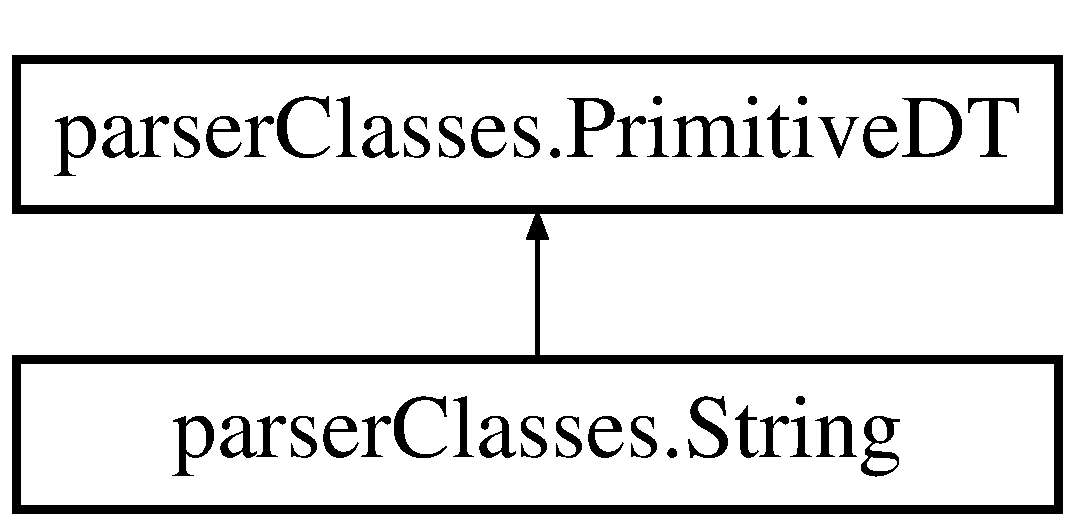
\includegraphics[height=2.000000cm]{classparser_classes_1_1_string}
\end{center}
\end{figure}
\subsection*{Public Member Functions}
\begin{DoxyCompactItemize}
\item 
\mbox{\Hypertarget{classparser_classes_1_1_string_a4c4e2819010c0c58d4f628f3584fdd69}\label{classparser_classes_1_1_string_a4c4e2819010c0c58d4f628f3584fdd69}} 
def {\bfseries \+\_\+\+\_\+init\+\_\+\+\_\+} (self, value=\textquotesingle{}\char`\"{}\char`\"{}\textquotesingle{})
\item 
\mbox{\Hypertarget{classparser_classes_1_1_string_a7a00e512a68ea3f88b25bcb060382393}\label{classparser_classes_1_1_string_a7a00e512a68ea3f88b25bcb060382393}} 
def {\bfseries give\+Type} (self)
\item 
\mbox{\Hypertarget{classparser_classes_1_1_string_a11c7326188baeb6a6e43a06d6f94d055}\label{classparser_classes_1_1_string_a11c7326188baeb6a6e43a06d6f94d055}} 
def {\bfseries update} (self, val)
\end{DoxyCompactItemize}
\subsection*{Public Attributes}
\begin{DoxyCompactItemize}
\item 
\mbox{\Hypertarget{classparser_classes_1_1_string_a04fcb7b360e30d106a7879b0964274b3}\label{classparser_classes_1_1_string_a04fcb7b360e30d106a7879b0964274b3}} 
{\bfseries value}
\end{DoxyCompactItemize}


The documentation for this class was generated from the following file\+:\begin{DoxyCompactItemize}
\item 
parser\+Classes.\+py\end{DoxyCompactItemize}

\hypertarget{class_parsing_classes_actual_1_1_string}{}\section{Parsing\+Classes\+Actual.\+String Class Reference}
\label{class_parsing_classes_actual_1_1_string}\index{Parsing\+Classes\+Actual.\+String@{Parsing\+Classes\+Actual.\+String}}


class for string datatype  


Inheritance diagram for Parsing\+Classes\+Actual.\+String\+:\begin{figure}[H]
\begin{center}
\leavevmode
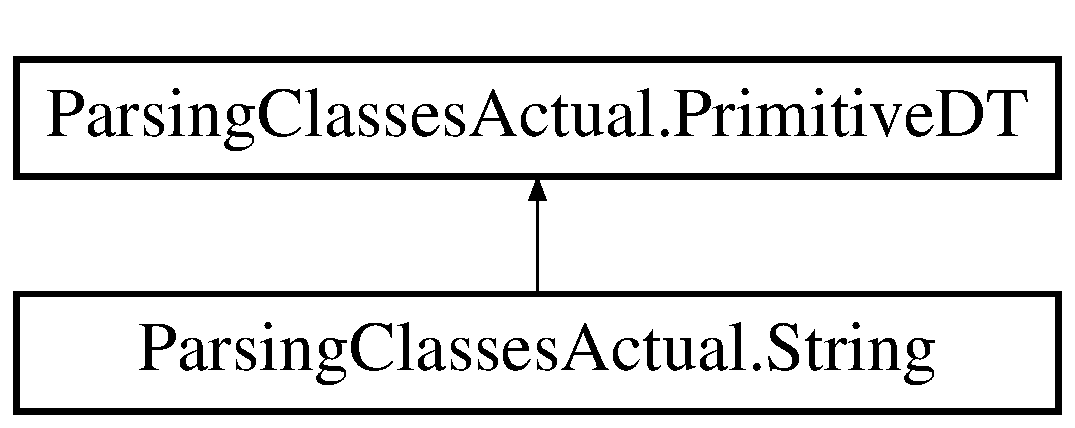
\includegraphics[height=2.000000cm]{class_parsing_classes_actual_1_1_string}
\end{center}
\end{figure}
\subsection*{Public Member Functions}
\begin{DoxyCompactItemize}
\item 
def \hyperlink{class_parsing_classes_actual_1_1_string_a8f97f0ea4e268f51804084ae84435c52}{\+\_\+\+\_\+init\+\_\+\+\_\+} (self, value=\textquotesingle{}\char`\"{}\char`\"{}\textquotesingle{})
\begin{DoxyCompactList}\small\item\em the constructor \end{DoxyCompactList}\item 
def \hyperlink{class_parsing_classes_actual_1_1_string_a292e4be2531c8eb3d6aa6f328defdad7}{give\+Type} (self)\hypertarget{class_parsing_classes_actual_1_1_string_a292e4be2531c8eb3d6aa6f328defdad7}{}\label{class_parsing_classes_actual_1_1_string_a292e4be2531c8eb3d6aa6f328defdad7}

\begin{DoxyCompactList}\small\item\em returns the type of value \end{DoxyCompactList}\item 
def \hyperlink{class_parsing_classes_actual_1_1_string_aa1f293f1e6aebb5522bb65ecfcce9051}{update} (self, val)\hypertarget{class_parsing_classes_actual_1_1_string_aa1f293f1e6aebb5522bb65ecfcce9051}{}\label{class_parsing_classes_actual_1_1_string_aa1f293f1e6aebb5522bb65ecfcce9051}

\begin{DoxyCompactList}\small\item\em updates the stored value by typecasting it \end{DoxyCompactList}\end{DoxyCompactItemize}
\subsection*{Public Attributes}
\begin{DoxyCompactItemize}
\item 
{\bfseries value}\hypertarget{class_parsing_classes_actual_1_1_string_a184687889206e8d800af3384c4c61265}{}\label{class_parsing_classes_actual_1_1_string_a184687889206e8d800af3384c4c61265}

\end{DoxyCompactItemize}


\subsection{Detailed Description}
class for string datatype 

\subsection{Constructor \& Destructor Documentation}
\index{Parsing\+Classes\+Actual\+::\+String@{Parsing\+Classes\+Actual\+::\+String}!\+\_\+\+\_\+init\+\_\+\+\_\+@{\+\_\+\+\_\+init\+\_\+\+\_\+}}
\index{\+\_\+\+\_\+init\+\_\+\+\_\+@{\+\_\+\+\_\+init\+\_\+\+\_\+}!Parsing\+Classes\+Actual\+::\+String@{Parsing\+Classes\+Actual\+::\+String}}
\subsubsection[{\texorpdfstring{\+\_\+\+\_\+init\+\_\+\+\_\+(self, value=\textquotesingle{}""""\textquotesingle{})}{__init__(self, value='""')}}]{\setlength{\rightskip}{0pt plus 5cm}def Parsing\+Classes\+Actual.\+String.\+\_\+\+\_\+init\+\_\+\+\_\+ (
\begin{DoxyParamCaption}
\item[{}]{self, }
\item[{}]{value = {\ttfamily \textquotesingle{}\char`\"{}\char`\"{}\textquotesingle{}}}
\end{DoxyParamCaption}
)}\hypertarget{class_parsing_classes_actual_1_1_string_a8f97f0ea4e268f51804084ae84435c52}{}\label{class_parsing_classes_actual_1_1_string_a8f97f0ea4e268f51804084ae84435c52}


the constructor 


\begin{DoxyParams}{Parameters}
{\em the} & value of datatype \\
\hline
\end{DoxyParams}


The documentation for this class was generated from the following file\+:\begin{DoxyCompactItemize}
\item 
Parsing\+Classes\+Actual.\+py\end{DoxyCompactItemize}

\hypertarget{class_parsing_classes_actual_1_1_term}{}\section{Parsing\+Classes\+Actual.\+Term Class Reference}
\label{class_parsing_classes_actual_1_1_term}\index{Parsing\+Classes\+Actual.\+Term@{Parsing\+Classes\+Actual.\+Term}}
\subsection*{Public Member Functions}
\begin{DoxyCompactItemize}
\item 
\mbox{\Hypertarget{class_parsing_classes_actual_1_1_term_a59155d0cbc1245f862052b47fd257739}\label{class_parsing_classes_actual_1_1_term_a59155d0cbc1245f862052b47fd257739}} 
def {\bfseries \+\_\+\+\_\+init\+\_\+\+\_\+} (self)
\item 
\mbox{\Hypertarget{class_parsing_classes_actual_1_1_term_adaa3917c680bb2cc250b23f02333f03a}\label{class_parsing_classes_actual_1_1_term_adaa3917c680bb2cc250b23f02333f03a}} 
def {\bfseries add\+Element} (self, element)
\item 
\mbox{\Hypertarget{class_parsing_classes_actual_1_1_term_a3fbb50911cfcdfdb1453c0882cf82cc5}\label{class_parsing_classes_actual_1_1_term_a3fbb50911cfcdfdb1453c0882cf82cc5}} 
def {\bfseries eval} (self)
\end{DoxyCompactItemize}
\subsection*{Public Attributes}
\begin{DoxyCompactItemize}
\item 
\mbox{\Hypertarget{class_parsing_classes_actual_1_1_term_a5281bd694526cb3549ca900f49628b51}\label{class_parsing_classes_actual_1_1_term_a5281bd694526cb3549ca900f49628b51}} 
{\bfseries elements}
\end{DoxyCompactItemize}


The documentation for this class was generated from the following file\+:\begin{DoxyCompactItemize}
\item 
Parsing\+Classes\+Actual.\+py\end{DoxyCompactItemize}

\hypertarget{classparser_classes_1_1_term}{}\section{parser\+Classes.\+Term Class Reference}
\label{classparser_classes_1_1_term}\index{parser\+Classes.\+Term@{parser\+Classes.\+Term}}
\subsection*{Public Member Functions}
\begin{DoxyCompactItemize}
\item 
def {\bfseries \+\_\+\+\_\+init\+\_\+\+\_\+} (self)\hypertarget{classparser_classes_1_1_term_a6c4e5a1df9a4e150418f70d649bb0ccf}{}\label{classparser_classes_1_1_term_a6c4e5a1df9a4e150418f70d649bb0ccf}

\item 
def {\bfseries add\+Element} (self, element)\hypertarget{classparser_classes_1_1_term_a61959371502fbe2ff800e1c105cc12aa}{}\label{classparser_classes_1_1_term_a61959371502fbe2ff800e1c105cc12aa}

\item 
def {\bfseries eval} (self)\hypertarget{classparser_classes_1_1_term_a59507b1f0f91fc82f9c152ee33a89251}{}\label{classparser_classes_1_1_term_a59507b1f0f91fc82f9c152ee33a89251}

\end{DoxyCompactItemize}
\subsection*{Public Attributes}
\begin{DoxyCompactItemize}
\item 
{\bfseries elements}\hypertarget{classparser_classes_1_1_term_ac347a45be39cbf864849da398d22d2d2}{}\label{classparser_classes_1_1_term_ac347a45be39cbf864849da398d22d2d2}

\end{DoxyCompactItemize}


The documentation for this class was generated from the following file\+:\begin{DoxyCompactItemize}
\item 
parser\+Classes.\+py\end{DoxyCompactItemize}

\hypertarget{classgraphics_1_1_text}{}\section{graphics.\+Text Class Reference}
\label{classgraphics_1_1_text}\index{graphics.\+Text@{graphics.\+Text}}
Inheritance diagram for graphics.\+Text\+:\begin{figure}[H]
\begin{center}
\leavevmode
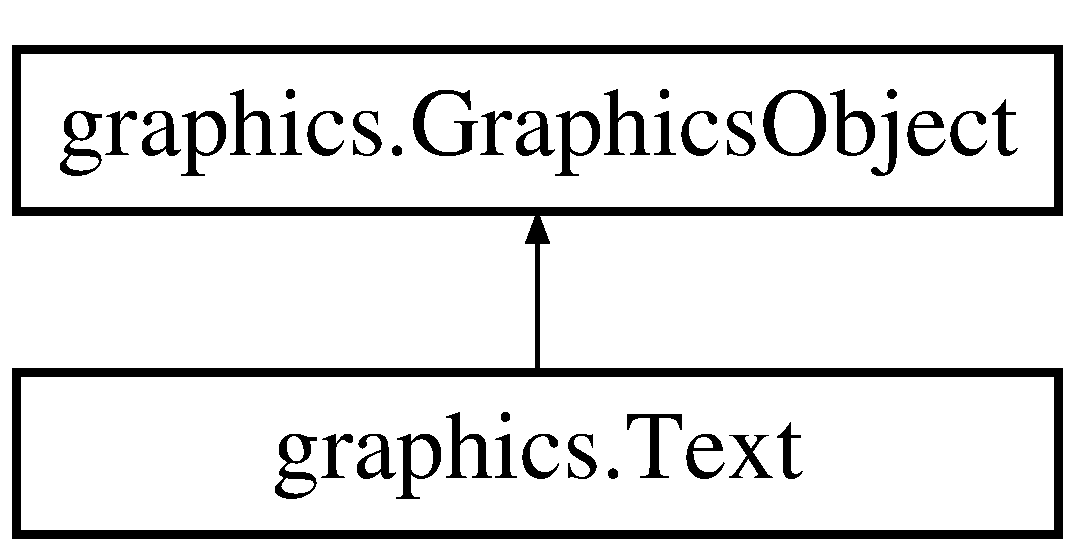
\includegraphics[height=2.000000cm]{classgraphics_1_1_text}
\end{center}
\end{figure}
\subsection*{Public Member Functions}
\begin{DoxyCompactItemize}
\item 
def {\bfseries \+\_\+\+\_\+init\+\_\+\+\_\+} (self, p, text)\hypertarget{classgraphics_1_1_text_af17676ed39bcc03a78098b22a15ef591}{}\label{classgraphics_1_1_text_af17676ed39bcc03a78098b22a15ef591}

\item 
def {\bfseries \+\_\+\+\_\+repr\+\_\+\+\_\+} (self)\hypertarget{classgraphics_1_1_text_ae0b4ff4a08c45410d4f424a48a6eba59}{}\label{classgraphics_1_1_text_ae0b4ff4a08c45410d4f424a48a6eba59}

\item 
def {\bfseries clone} (self)\hypertarget{classgraphics_1_1_text_a507a4eea3a7a7de19bfe30ff70cf8fd6}{}\label{classgraphics_1_1_text_a507a4eea3a7a7de19bfe30ff70cf8fd6}

\item 
def {\bfseries set\+Text} (self, text)\hypertarget{classgraphics_1_1_text_ab8a97b69fe919acb98429b7da81b7d37}{}\label{classgraphics_1_1_text_ab8a97b69fe919acb98429b7da81b7d37}

\item 
def {\bfseries get\+Text} (self)\hypertarget{classgraphics_1_1_text_a1697a465c237e26532f43cef1af6abe5}{}\label{classgraphics_1_1_text_a1697a465c237e26532f43cef1af6abe5}

\item 
def {\bfseries get\+Anchor} (self)\hypertarget{classgraphics_1_1_text_a02525bc36e0af653d17905cd733d0843}{}\label{classgraphics_1_1_text_a02525bc36e0af653d17905cd733d0843}

\item 
def {\bfseries set\+Face} (self, face)\hypertarget{classgraphics_1_1_text_ae58860c5531b95e69136a819489a3169}{}\label{classgraphics_1_1_text_ae58860c5531b95e69136a819489a3169}

\item 
def {\bfseries set\+Size} (self, size)\hypertarget{classgraphics_1_1_text_a31ea18b7a09603cdb49a4716290ec8fe}{}\label{classgraphics_1_1_text_a31ea18b7a09603cdb49a4716290ec8fe}

\item 
def {\bfseries set\+Style} (self, style)\hypertarget{classgraphics_1_1_text_af2697684710c7471abe9bc8bf0f5fffe}{}\label{classgraphics_1_1_text_af2697684710c7471abe9bc8bf0f5fffe}

\item 
def {\bfseries set\+Text\+Color} (self, color)\hypertarget{classgraphics_1_1_text_a4ee730f2d0f9a81250b8ca232940fec8}{}\label{classgraphics_1_1_text_a4ee730f2d0f9a81250b8ca232940fec8}

\end{DoxyCompactItemize}
\subsection*{Public Attributes}
\begin{DoxyCompactItemize}
\item 
{\bfseries anchor}\hypertarget{classgraphics_1_1_text_a24a6cb5416b56cc809da0a358de69db7}{}\label{classgraphics_1_1_text_a24a6cb5416b56cc809da0a358de69db7}

\item 
{\bfseries set\+Outline}\hypertarget{classgraphics_1_1_text_a9b7d6fa2325a028c73778227d8f9ac99}{}\label{classgraphics_1_1_text_a9b7d6fa2325a028c73778227d8f9ac99}

\end{DoxyCompactItemize}


The documentation for this class was generated from the following file\+:\begin{DoxyCompactItemize}
\item 
graphics.\+py\end{DoxyCompactItemize}

\hypertarget{classgraphics_1_1_transform}{}\section{graphics.\+Transform Class Reference}
\label{classgraphics_1_1_transform}\index{graphics.\+Transform@{graphics.\+Transform}}
\subsection*{Public Member Functions}
\begin{DoxyCompactItemize}
\item 
def {\bfseries \+\_\+\+\_\+init\+\_\+\+\_\+} (self, w, h, xlow, ylow, xhigh, yhigh)\hypertarget{classgraphics_1_1_transform_a826600468986f5938247b1a09dc89097}{}\label{classgraphics_1_1_transform_a826600468986f5938247b1a09dc89097}

\item 
def {\bfseries screen} (self, x, y)\hypertarget{classgraphics_1_1_transform_a52ce3f42703299dcf57d65dbdf856ccc}{}\label{classgraphics_1_1_transform_a52ce3f42703299dcf57d65dbdf856ccc}

\item 
def {\bfseries world} (self, xs, ys)\hypertarget{classgraphics_1_1_transform_adaa57283f32d487d122a5cae919ce1e8}{}\label{classgraphics_1_1_transform_adaa57283f32d487d122a5cae919ce1e8}

\end{DoxyCompactItemize}
\subsection*{Public Attributes}
\begin{DoxyCompactItemize}
\item 
{\bfseries xbase}\hypertarget{classgraphics_1_1_transform_af43d705e45fda80627425215440a0394}{}\label{classgraphics_1_1_transform_af43d705e45fda80627425215440a0394}

\item 
{\bfseries ybase}\hypertarget{classgraphics_1_1_transform_a56bedbb5d2c98e6bf4f1ac28b77688d5}{}\label{classgraphics_1_1_transform_a56bedbb5d2c98e6bf4f1ac28b77688d5}

\item 
{\bfseries xscale}\hypertarget{classgraphics_1_1_transform_aa5d63ba571985d5d70ee661b7e84646f}{}\label{classgraphics_1_1_transform_aa5d63ba571985d5d70ee661b7e84646f}

\item 
{\bfseries yscale}\hypertarget{classgraphics_1_1_transform_aad8322957fc2e0f6b445440f04150c1d}{}\label{classgraphics_1_1_transform_aad8322957fc2e0f6b445440f04150c1d}

\end{DoxyCompactItemize}


\subsection{Detailed Description}
\begin{DoxyVerb}Internal class for 2-D coordinate transformations\end{DoxyVerb}
 

The documentation for this class was generated from the following file\+:\begin{DoxyCompactItemize}
\item 
graphics.\+py\end{DoxyCompactItemize}

\hypertarget{classparser_classes_1_1_unary_op}{}\section{parser\+Classes.\+Unary\+Op Class Reference}
\label{classparser_classes_1_1_unary_op}\index{parser\+Classes.\+Unary\+Op@{parser\+Classes.\+Unary\+Op}}


class for unary op with function and operand  


\subsection*{Public Member Functions}
\begin{DoxyCompactItemize}
\item 
def {\bfseries \+\_\+\+\_\+init\+\_\+\+\_\+} (self, operator, operand)\hypertarget{classparser_classes_1_1_unary_op_acd865fc282d065da966ee8ae6fd1221c}{}\label{classparser_classes_1_1_unary_op_acd865fc282d065da966ee8ae6fd1221c}

\item 
def {\bfseries eval} (self)\hypertarget{classparser_classes_1_1_unary_op_a3bcb0143d84e533f554616cf279910c1}{}\label{classparser_classes_1_1_unary_op_a3bcb0143d84e533f554616cf279910c1}

\item 
def {\bfseries get\+Operator} (self)\hypertarget{classparser_classes_1_1_unary_op_afa168433abdb12ff7376e1bfe4f6d347}{}\label{classparser_classes_1_1_unary_op_afa168433abdb12ff7376e1bfe4f6d347}

\end{DoxyCompactItemize}
\subsection*{Public Attributes}
\begin{DoxyCompactItemize}
\item 
{\bfseries operator}\hypertarget{classparser_classes_1_1_unary_op_a5207cf805eeb0fb6dc3386378216600d}{}\label{classparser_classes_1_1_unary_op_a5207cf805eeb0fb6dc3386378216600d}

\item 
{\bfseries operand}\hypertarget{classparser_classes_1_1_unary_op_a45cebabb240f349eb45b24331bb6323c}{}\label{classparser_classes_1_1_unary_op_a45cebabb240f349eb45b24331bb6323c}

\end{DoxyCompactItemize}


\subsection{Detailed Description}
class for unary op with function and operand 

The documentation for this class was generated from the following file\+:\begin{DoxyCompactItemize}
\item 
parser\+Classes.\+py\end{DoxyCompactItemize}

\hypertarget{class_parsing_classes_actual_1_1_unary_op}{}\section{Parsing\+Classes\+Actual.\+Unary\+Op Class Reference}
\label{class_parsing_classes_actual_1_1_unary_op}\index{Parsing\+Classes\+Actual.\+Unary\+Op@{Parsing\+Classes\+Actual.\+Unary\+Op}}


class for unary op with function and operand  


\subsection*{Public Member Functions}
\begin{DoxyCompactItemize}
\item 
def \hyperlink{class_parsing_classes_actual_1_1_unary_op_ae822716a1ac45674aa119773fb9eb0aa}{\+\_\+\+\_\+init\+\_\+\+\_\+} (self, operator, operand, snippet)
\begin{DoxyCompactList}\small\item\em the constructor \end{DoxyCompactList}\item 
def \hyperlink{class_parsing_classes_actual_1_1_unary_op_a825795bcc2929152bb0ca9618ab419ad}{eval} (self)\hypertarget{class_parsing_classes_actual_1_1_unary_op_a825795bcc2929152bb0ca9618ab419ad}{}\label{class_parsing_classes_actual_1_1_unary_op_a825795bcc2929152bb0ca9618ab419ad}

\begin{DoxyCompactList}\small\item\em Evaluates the expression. \end{DoxyCompactList}\item 
def \hyperlink{class_parsing_classes_actual_1_1_unary_op_a708a1db9dea33517c487d535082c49c4}{get\+Operator} (self)\hypertarget{class_parsing_classes_actual_1_1_unary_op_a708a1db9dea33517c487d535082c49c4}{}\label{class_parsing_classes_actual_1_1_unary_op_a708a1db9dea33517c487d535082c49c4}

\begin{DoxyCompactList}\small\item\em Gives the type of operator. \end{DoxyCompactList}\end{DoxyCompactItemize}
\subsection*{Public Attributes}
\begin{DoxyCompactItemize}
\item 
{\bfseries operator}\hypertarget{class_parsing_classes_actual_1_1_unary_op_afb0d7cdde99cb150d27d101f00fbf275}{}\label{class_parsing_classes_actual_1_1_unary_op_afb0d7cdde99cb150d27d101f00fbf275}

\item 
{\bfseries operand}\hypertarget{class_parsing_classes_actual_1_1_unary_op_a34fbc9a5ae586ae2640a00777b23a090}{}\label{class_parsing_classes_actual_1_1_unary_op_a34fbc9a5ae586ae2640a00777b23a090}

\item 
{\bfseries snippet}\hypertarget{class_parsing_classes_actual_1_1_unary_op_ab8b505d37c98c26e98376ed18b5999d2}{}\label{class_parsing_classes_actual_1_1_unary_op_ab8b505d37c98c26e98376ed18b5999d2}

\end{DoxyCompactItemize}


\subsection{Detailed Description}
class for unary op with function and operand 

\subsection{Constructor \& Destructor Documentation}
\index{Parsing\+Classes\+Actual\+::\+Unary\+Op@{Parsing\+Classes\+Actual\+::\+Unary\+Op}!\+\_\+\+\_\+init\+\_\+\+\_\+@{\+\_\+\+\_\+init\+\_\+\+\_\+}}
\index{\+\_\+\+\_\+init\+\_\+\+\_\+@{\+\_\+\+\_\+init\+\_\+\+\_\+}!Parsing\+Classes\+Actual\+::\+Unary\+Op@{Parsing\+Classes\+Actual\+::\+Unary\+Op}}
\subsubsection[{\texorpdfstring{\+\_\+\+\_\+init\+\_\+\+\_\+(self, operator, operand, snippet)}{__init__(self, operator, operand, snippet)}}]{\setlength{\rightskip}{0pt plus 5cm}def Parsing\+Classes\+Actual.\+Unary\+Op.\+\_\+\+\_\+init\+\_\+\+\_\+ (
\begin{DoxyParamCaption}
\item[{}]{self, }
\item[{}]{operator, }
\item[{}]{operand, }
\item[{}]{snippet}
\end{DoxyParamCaption}
)}\hypertarget{class_parsing_classes_actual_1_1_unary_op_ae822716a1ac45674aa119773fb9eb0aa}{}\label{class_parsing_classes_actual_1_1_unary_op_ae822716a1ac45674aa119773fb9eb0aa}


the constructor 


\begin{DoxyParams}{Parameters}
{\em operator} & The unary op \\
\hline
{\em operand} & The operand \\
\hline
{\em snippet} & The relevant code snippet \\
\hline
\end{DoxyParams}


The documentation for this class was generated from the following file\+:\begin{DoxyCompactItemize}
\item 
Parsing\+Classes\+Actual.\+py\end{DoxyCompactItemize}

\hypertarget{class_parsing_classes_actual_1_1_unknown__type}{}\section{Parsing\+Classes\+Actual.\+Unknown\+\_\+type Class Reference}
\label{class_parsing_classes_actual_1_1_unknown__type}\index{Parsing\+Classes\+Actual.\+Unknown\+\_\+type@{Parsing\+Classes\+Actual.\+Unknown\+\_\+type}}
\subsection*{Public Member Functions}
\begin{DoxyCompactItemize}
\item 
def {\bfseries \+\_\+\+\_\+init\+\_\+\+\_\+} (self, value)\hypertarget{class_parsing_classes_actual_1_1_unknown__type_ab7bc9b4c235952c48078cba856dcc317}{}\label{class_parsing_classes_actual_1_1_unknown__type_ab7bc9b4c235952c48078cba856dcc317}

\item 
def {\bfseries eval} (self)\hypertarget{class_parsing_classes_actual_1_1_unknown__type_a7273966f0982773d6904a4318854c787}{}\label{class_parsing_classes_actual_1_1_unknown__type_a7273966f0982773d6904a4318854c787}

\end{DoxyCompactItemize}
\subsection*{Public Attributes}
\begin{DoxyCompactItemize}
\item 
{\bfseries value}\hypertarget{class_parsing_classes_actual_1_1_unknown__type_ade1dc926e512e4485d163e92b6df182d}{}\label{class_parsing_classes_actual_1_1_unknown__type_ade1dc926e512e4485d163e92b6df182d}

\end{DoxyCompactItemize}


The documentation for this class was generated from the following file\+:\begin{DoxyCompactItemize}
\item 
Parsing\+Classes\+Actual.\+py\end{DoxyCompactItemize}

\hypertarget{classparser_classes_1_1_unknown__type}{}\section{parser\+Classes.\+Unknown\+\_\+type Class Reference}
\label{classparser_classes_1_1_unknown__type}\index{parser\+Classes.\+Unknown\+\_\+type@{parser\+Classes.\+Unknown\+\_\+type}}
\subsection*{Public Member Functions}
\begin{DoxyCompactItemize}
\item 
\mbox{\Hypertarget{classparser_classes_1_1_unknown__type_a9562f0bab5ec63025079c370fc164f81}\label{classparser_classes_1_1_unknown__type_a9562f0bab5ec63025079c370fc164f81}} 
def {\bfseries \+\_\+\+\_\+init\+\_\+\+\_\+} (self, value)
\item 
\mbox{\Hypertarget{classparser_classes_1_1_unknown__type_a28e421b5d0e2a0f7fcf34dae75ac51b4}\label{classparser_classes_1_1_unknown__type_a28e421b5d0e2a0f7fcf34dae75ac51b4}} 
def {\bfseries eval} (self)
\end{DoxyCompactItemize}
\subsection*{Public Attributes}
\begin{DoxyCompactItemize}
\item 
\mbox{\Hypertarget{classparser_classes_1_1_unknown__type_a35589b9171b9277aa83a08ca38c10938}\label{classparser_classes_1_1_unknown__type_a35589b9171b9277aa83a08ca38c10938}} 
{\bfseries value}
\end{DoxyCompactItemize}


The documentation for this class was generated from the following file\+:\begin{DoxyCompactItemize}
\item 
parser\+Classes.\+py\end{DoxyCompactItemize}

\hypertarget{classparser_classes_1_1_variable}{}\section{parser\+Classes.\+Variable Class Reference}
\label{classparser_classes_1_1_variable}\index{parser\+Classes.\+Variable@{parser\+Classes.\+Variable}}
\subsection*{Public Member Functions}
\begin{DoxyCompactItemize}
\item 
def {\bfseries \+\_\+\+\_\+init\+\_\+\+\_\+} (self, name)\hypertarget{classparser_classes_1_1_variable_a96d789a80a5bcb1246ddcf6ff9a53fd5}{}\label{classparser_classes_1_1_variable_a96d789a80a5bcb1246ddcf6ff9a53fd5}

\item 
def {\bfseries eval} (self)\hypertarget{classparser_classes_1_1_variable_a252b110790e003233c628e748f620fc1}{}\label{classparser_classes_1_1_variable_a252b110790e003233c628e748f620fc1}

\item 
def {\bfseries update} (self, obj2)\hypertarget{classparser_classes_1_1_variable_a53b0e8b8172450a6d2200161a6706118}{}\label{classparser_classes_1_1_variable_a53b0e8b8172450a6d2200161a6706118}

\end{DoxyCompactItemize}
\subsection*{Public Attributes}
\begin{DoxyCompactItemize}
\item 
{\bfseries name}\hypertarget{classparser_classes_1_1_variable_aab7cba9066f629ddacf7c6fc13413979}{}\label{classparser_classes_1_1_variable_aab7cba9066f629ddacf7c6fc13413979}

\end{DoxyCompactItemize}


The documentation for this class was generated from the following file\+:\begin{DoxyCompactItemize}
\item 
parser\+Classes.\+py\end{DoxyCompactItemize}

\hypertarget{class_parsing_classes_actual_1_1_variable}{}\section{Parsing\+Classes\+Actual.\+Variable Class Reference}
\label{class_parsing_classes_actual_1_1_variable}\index{Parsing\+Classes\+Actual.\+Variable@{Parsing\+Classes\+Actual.\+Variable}}


The class which stores a variable as a class,with relevant functions like eval and update.  


\subsection*{Public Member Functions}
\begin{DoxyCompactItemize}
\item 
def \hyperlink{class_parsing_classes_actual_1_1_variable_a1e45d0c6cdb70b7f36a432914a530364}{\+\_\+\+\_\+init\+\_\+\+\_\+} (self, name)
\begin{DoxyCompactList}\small\item\em the constructor \end{DoxyCompactList}\item 
\mbox{\Hypertarget{class_parsing_classes_actual_1_1_variable_ad10453c7fa8c6067a3e20ca7b15a9b0e}\label{class_parsing_classes_actual_1_1_variable_ad10453c7fa8c6067a3e20ca7b15a9b0e}} 
def \hyperlink{class_parsing_classes_actual_1_1_variable_ad10453c7fa8c6067a3e20ca7b15a9b0e}{eval} (self)
\begin{DoxyCompactList}\small\item\em The value of the the variable is given after looking up the dictionary. \end{DoxyCompactList}\item 
def \hyperlink{class_parsing_classes_actual_1_1_variable_ac3a39c7351d2b51b097903733af3f7ec}{update} (self, obj2)
\begin{DoxyCompactList}\small\item\em It updates the value of the variable. \end{DoxyCompactList}\end{DoxyCompactItemize}
\subsection*{Public Attributes}
\begin{DoxyCompactItemize}
\item 
\mbox{\Hypertarget{class_parsing_classes_actual_1_1_variable_ada0de9ca99f5a48b167a472f2f03d100}\label{class_parsing_classes_actual_1_1_variable_ada0de9ca99f5a48b167a472f2f03d100}} 
{\bfseries name}
\end{DoxyCompactItemize}


\subsection{Detailed Description}
The class which stores a variable as a class,with relevant functions like eval and update. 

\subsection{Constructor \& Destructor Documentation}
\mbox{\Hypertarget{class_parsing_classes_actual_1_1_variable_a1e45d0c6cdb70b7f36a432914a530364}\label{class_parsing_classes_actual_1_1_variable_a1e45d0c6cdb70b7f36a432914a530364}} 
\index{Parsing\+Classes\+Actual\+::\+Variable@{Parsing\+Classes\+Actual\+::\+Variable}!\+\_\+\+\_\+init\+\_\+\+\_\+@{\+\_\+\+\_\+init\+\_\+\+\_\+}}
\index{\+\_\+\+\_\+init\+\_\+\+\_\+@{\+\_\+\+\_\+init\+\_\+\+\_\+}!Parsing\+Classes\+Actual\+::\+Variable@{Parsing\+Classes\+Actual\+::\+Variable}}
\subsubsection{\texorpdfstring{\+\_\+\+\_\+init\+\_\+\+\_\+()}{\_\_init\_\_()}}
{\footnotesize\ttfamily def Parsing\+Classes\+Actual.\+Variable.\+\_\+\+\_\+init\+\_\+\+\_\+ (\begin{DoxyParamCaption}\item[{}]{self,  }\item[{}]{name }\end{DoxyParamCaption})}



the constructor 


\begin{DoxyParams}{Parameters}
{\em name} & The name of the variable being stored \\
\hline
\end{DoxyParams}


\subsection{Member Function Documentation}
\mbox{\Hypertarget{class_parsing_classes_actual_1_1_variable_ac3a39c7351d2b51b097903733af3f7ec}\label{class_parsing_classes_actual_1_1_variable_ac3a39c7351d2b51b097903733af3f7ec}} 
\index{Parsing\+Classes\+Actual\+::\+Variable@{Parsing\+Classes\+Actual\+::\+Variable}!update@{update}}
\index{update@{update}!Parsing\+Classes\+Actual\+::\+Variable@{Parsing\+Classes\+Actual\+::\+Variable}}
\subsubsection{\texorpdfstring{update()}{update()}}
{\footnotesize\ttfamily def Parsing\+Classes\+Actual.\+Variable.\+update (\begin{DoxyParamCaption}\item[{}]{self,  }\item[{}]{obj2 }\end{DoxyParamCaption})}



It updates the value of the variable. 


\begin{DoxyParams}{Parameters}
{\em obj2} & The value(a class to be evaluated) to which the updation has to occur \\
\hline
\end{DoxyParams}


The documentation for this class was generated from the following file\+:\begin{DoxyCompactItemize}
\item 
Parsing\+Classes\+Actual.\+py\end{DoxyCompactItemize}

\hypertarget{classexecution_stack_1_1_visual_array}{}\section{execution\+Stack.\+Visual\+Array Class Reference}
\label{classexecution_stack_1_1_visual_array}\index{execution\+Stack.\+Visual\+Array@{execution\+Stack.\+Visual\+Array}}
\subsection*{Public Member Functions}
\begin{DoxyCompactItemize}
\item 
def {\bfseries \+\_\+\+\_\+init\+\_\+\+\_\+} (self, size, name)\hypertarget{classexecution_stack_1_1_visual_array_ad98c3e54817417c582a6244b73aa7dff}{}\label{classexecution_stack_1_1_visual_array_ad98c3e54817417c582a6244b73aa7dff}

\item 
def {\bfseries update} (self, index, val)\hypertarget{classexecution_stack_1_1_visual_array_a627f6a007e0ba27e135794ffcd19ed5a}{}\label{classexecution_stack_1_1_visual_array_a627f6a007e0ba27e135794ffcd19ed5a}

\item 
def {\bfseries probe} (self, index)\hypertarget{classexecution_stack_1_1_visual_array_adb38a0d313aa12b116095516798180f7}{}\label{classexecution_stack_1_1_visual_array_adb38a0d313aa12b116095516798180f7}

\item 
def {\bfseries delete} (self)\hypertarget{classexecution_stack_1_1_visual_array_ae62023d197eed6af549d467433b755f2}{}\label{classexecution_stack_1_1_visual_array_ae62023d197eed6af549d467433b755f2}

\end{DoxyCompactItemize}
\subsection*{Public Attributes}
\begin{DoxyCompactItemize}
\item 
{\bfseries name}\hypertarget{classexecution_stack_1_1_visual_array_a023a4ef16ccae091bef57d53e2a51dae}{}\label{classexecution_stack_1_1_visual_array_a023a4ef16ccae091bef57d53e2a51dae}

\item 
{\bfseries y}\hypertarget{classexecution_stack_1_1_visual_array_ab3f2e9efc42105c4331895a70a8b4eee}{}\label{classexecution_stack_1_1_visual_array_ab3f2e9efc42105c4331895a70a8b4eee}

\item 
{\bfseries x}\hypertarget{classexecution_stack_1_1_visual_array_a39c643fa75477c85f01f9e1b0108f353}{}\label{classexecution_stack_1_1_visual_array_a39c643fa75477c85f01f9e1b0108f353}

\item 
{\bfseries name\+Text}\hypertarget{classexecution_stack_1_1_visual_array_a8d513f04c041be10b60a472341aca538}{}\label{classexecution_stack_1_1_visual_array_a8d513f04c041be10b60a472341aca538}

\item 
{\bfseries size}\hypertarget{classexecution_stack_1_1_visual_array_a5498a6092e7d281cd651139137aa4bc7}{}\label{classexecution_stack_1_1_visual_array_a5498a6092e7d281cd651139137aa4bc7}

\item 
{\bfseries array}\hypertarget{classexecution_stack_1_1_visual_array_af9ff7cb5547d5a4f85a49350ff4fdef7}{}\label{classexecution_stack_1_1_visual_array_af9ff7cb5547d5a4f85a49350ff4fdef7}

\end{DoxyCompactItemize}


The documentation for this class was generated from the following file\+:\begin{DoxyCompactItemize}
\item 
execution\+Stack.\+py\end{DoxyCompactItemize}

\hypertarget{classparser_classes_1_1_while_loop}{}\section{parser\+Classes.\+While\+Loop Class Reference}
\label{classparser_classes_1_1_while_loop}\index{parser\+Classes.\+While\+Loop@{parser\+Classes.\+While\+Loop}}
\subsection*{Public Member Functions}
\begin{DoxyCompactItemize}
\item 
def {\bfseries \+\_\+\+\_\+init\+\_\+\+\_\+} (self, express, statement\+List)\hypertarget{classparser_classes_1_1_while_loop_a886ffecb17b87a41ec66691dead4da00}{}\label{classparser_classes_1_1_while_loop_a886ffecb17b87a41ec66691dead4da00}

\item 
def {\bfseries exec} (self)\hypertarget{classparser_classes_1_1_while_loop_a8f1705d74c2e71c1cb37398d33261442}{}\label{classparser_classes_1_1_while_loop_a8f1705d74c2e71c1cb37398d33261442}

\end{DoxyCompactItemize}
\subsection*{Public Attributes}
\begin{DoxyCompactItemize}
\item 
{\bfseries express}\hypertarget{classparser_classes_1_1_while_loop_aadd614a12b85a9536c5cb231eb60a579}{}\label{classparser_classes_1_1_while_loop_aadd614a12b85a9536c5cb231eb60a579}

\item 
{\bfseries statement\+List}\hypertarget{classparser_classes_1_1_while_loop_aef24cd7f0ead40a82bbad44af58890c1}{}\label{classparser_classes_1_1_while_loop_aef24cd7f0ead40a82bbad44af58890c1}

\end{DoxyCompactItemize}


The documentation for this class was generated from the following file\+:\begin{DoxyCompactItemize}
\item 
parser\+Classes.\+py\end{DoxyCompactItemize}

\hypertarget{class_parsing_classes_actual_1_1_while_loop}{}\section{Parsing\+Classes\+Actual.\+While\+Loop Class Reference}
\label{class_parsing_classes_actual_1_1_while_loop}\index{Parsing\+Classes\+Actual.\+While\+Loop@{Parsing\+Classes\+Actual.\+While\+Loop}}


similar to for-\/loop having required arguements  


\subsection*{Public Member Functions}
\begin{DoxyCompactItemize}
\item 
def \hyperlink{class_parsing_classes_actual_1_1_while_loop_adf4ccccee2acf19cea376f4ebb9dfd66}{\+\_\+\+\_\+init\+\_\+\+\_\+} (self, express, statement\+List, snippet)
\begin{DoxyCompactList}\small\item\em the constructor \end{DoxyCompactList}\item 
\mbox{\Hypertarget{class_parsing_classes_actual_1_1_while_loop_a458309ab7ca3701811c3561488ad2940}\label{class_parsing_classes_actual_1_1_while_loop_a458309ab7ca3701811c3561488ad2940}} 
def \hyperlink{class_parsing_classes_actual_1_1_while_loop_a458309ab7ca3701811c3561488ad2940}{exec} (self)
\begin{DoxyCompactList}\small\item\em the ecutable implementing While-\/loop \end{DoxyCompactList}\end{DoxyCompactItemize}
\subsection*{Public Attributes}
\begin{DoxyCompactItemize}
\item 
\mbox{\Hypertarget{class_parsing_classes_actual_1_1_while_loop_a81fb2f8bd34b6e7a3e31a1afa5331cb5}\label{class_parsing_classes_actual_1_1_while_loop_a81fb2f8bd34b6e7a3e31a1afa5331cb5}} 
{\bfseries express}
\item 
\mbox{\Hypertarget{class_parsing_classes_actual_1_1_while_loop_a0274f797bd8e0c3a3e260796acf14d6d}\label{class_parsing_classes_actual_1_1_while_loop_a0274f797bd8e0c3a3e260796acf14d6d}} 
{\bfseries statement\+List}
\item 
\mbox{\Hypertarget{class_parsing_classes_actual_1_1_while_loop_a1c7300045f672d208fdee2f590bb5084}\label{class_parsing_classes_actual_1_1_while_loop_a1c7300045f672d208fdee2f590bb5084}} 
{\bfseries snippet}
\end{DoxyCompactItemize}


\subsection{Detailed Description}
similar to for-\/loop having required arguements 

\subsection{Constructor \& Destructor Documentation}
\mbox{\Hypertarget{class_parsing_classes_actual_1_1_while_loop_adf4ccccee2acf19cea376f4ebb9dfd66}\label{class_parsing_classes_actual_1_1_while_loop_adf4ccccee2acf19cea376f4ebb9dfd66}} 
\index{Parsing\+Classes\+Actual\+::\+While\+Loop@{Parsing\+Classes\+Actual\+::\+While\+Loop}!\+\_\+\+\_\+init\+\_\+\+\_\+@{\+\_\+\+\_\+init\+\_\+\+\_\+}}
\index{\+\_\+\+\_\+init\+\_\+\+\_\+@{\+\_\+\+\_\+init\+\_\+\+\_\+}!Parsing\+Classes\+Actual\+::\+While\+Loop@{Parsing\+Classes\+Actual\+::\+While\+Loop}}
\subsubsection{\texorpdfstring{\+\_\+\+\_\+init\+\_\+\+\_\+()}{\_\_init\_\_()}}
{\footnotesize\ttfamily def Parsing\+Classes\+Actual.\+While\+Loop.\+\_\+\+\_\+init\+\_\+\+\_\+ (\begin{DoxyParamCaption}\item[{}]{self,  }\item[{}]{express,  }\item[{}]{statement\+List,  }\item[{}]{snippet }\end{DoxyParamCaption})}



the constructor 


\begin{DoxyParams}{Parameters}
{\em express} & The condition to be checked \\
\hline
{\em statement\+List} & The body of the for loop \\
\hline
{\em snippet} & The relevant code snippet \\
\hline
\end{DoxyParams}


The documentation for this class was generated from the following file\+:\begin{DoxyCompactItemize}
\item 
Parsing\+Classes\+Actual.\+py\end{DoxyCompactItemize}

%--- End generated contents ---

% Index
\backmatter
\newpage
\phantomsection
\clearemptydoublepage
\addcontentsline{toc}{chapter}{Index}
\printindex

\end{document}
